% 默认单面打印 oneside 、硕士论文模板 master
% 双面为 twoside

\documentclass[oneside, master, normal]{BIT-thesis-grd-jdh}

% 模板选项: 硕士论文 master; 博士论文 doctor
% 正常模式:normal  自查重模式:selfSimilarCheck  盲审模式:blindCheck
% 提交学校的查重文件可以直接使用normal模式结果
% 自查重模式主要用于关闭图片、公式等内容的显示,以减少文章字符数和降低PDF转word过程中出现的乱码,节省查重费用支出。应结合\insertcontents系列命令使用。对于土豪此选项没有任何卵用。。。。。
% 盲审模式主要根据盲审文件格式要求,隐去了作者、导师、致谢等信息,更改发表论文的格式

\usepackage{amsmath, bm}
\usepackage[ruled,linesnumbered,boxed]{algorithm2e}
\usepackage{makecell}
\setitemize{itemsep=0pt,partopsep=0pt,parsep=\parskip,topsep=0pt}
\setenumerate{itemsep=0pt,partopsep=0pt,parsep=\parskip,topsep=0pt}
\hyphenpenalty=5000
\tolerance=1000

\begin{document}

%%%%%%%%%%%%%%%%%%%%%%%%%%%%%%
%% 封面
%%%%%%%%%%%%%%%%%%%%%%%%%%%%%%

% 中文封面内容(关注内容而不是表现形式)
\classification{TP393.0} %可参考http://www.clcindex.com/category/TP/
\UDC{004.77} %可参考http://www.udcsummary.info/php/index.php?tag=0&lang=chi

\title{基于主动丢包的VoLTE时间隐通道构建方法研究}
\vtitle{基于主动丢包的\makeVerticalenWords{VoLTE}时间隐通道构建方法研究}
\author{徐欣廷}
\institute{计算机学院}
\advisor{谭毓安教授}
\chairman{张常有研究员}
\degree{工学硕士}
\major{计算机科学与技术}
\school{北京理工大学}
\defenddate{2020年6月}
%\studentnumber{**********}
\security{内部五年}


% 英文封面内容(关注内容而不是表现形式)
\englishtitle{Building Covert Timing Channels over VoLTE via Packet Dropout}
\englishauthor{Xinting Xu}
\englishadvisor{Prof. Yu-an Tan}
\englishchairman{Prof. Changyou Zhang}
\englishschool{Beijing Institute of Technology}
\englishinstitute{School of Computer Science and Technology}
\englishdegree{Master of Science}
\englishmajor{Computer Science and Technology}
\englishdate{June, 2020}

% 封面绘制
\maketitle

% 中文信息
\makeChineseInfo

% 英文信息
\makeEnglishInfo

%打印竖排论文题目
\makeVerticalTitle

% 论文原创性声明和使用授权
\makeDeclareOriginal

%%%%%%%%%%%%%%%%%%%%%%%%%%%%%%
%% 前置部分
%%%%%%%%%%%%%%%%%%%%%%%%%%%%%%
\frontmatter

% 摘要
%%==================================================
%% abstract.tex for BIT Master Thesis
%% modified by Xinting Xu
%% version: 0.1
%% last update: 2020-03-06
%%==================================================

\begin{abstract}
%本文的主要研究工作,是在VoLTE场景下,通过主动丢包的方式,构造安全、鲁棒的时间隐通道。伴随着第4代通信技术的应用,基于数据包交换的VoLTE(Voice over LTE)技术,取代了基于电路交换的传统通话技术。得益于LTE网络的高带宽、流量细分能力,VoLTE不仅为用户提供了低延迟、高清晰度的语音通话,也将低延迟的视频通话变为可能。
%借助实时传输协议RTP(Real-time Transport Protocol),VoLTE音视频数据被切分为独立的流,利用数据包优先级的差异,在保证传输效果的同时,提高抗干扰能力。对于语音数据流来说,基带内集成的信号采集单元,直接将编码后的数据打包为RTP数据包,经LTE组件发送到基站进行传输。另一方面,视频数据的来源是智能终端的摄像头模块,需要由应用处理器完成图像信息采集、压缩、编码,并按照RTP格式进行打包,最终交付基带处理器进行发送。

%由于处理途径及优先级方面的差异,数量较少的语音数据包,能够保持稳定且低丢包率的传输效果;而数量众多的视频数据包,受空口噪声的干扰,产生丢包现象不可避免。另一方面,VoLTE的通话双方均为无线终端,两侧的噪声强度和干扰阶段是不同的,丢包事件可能发生于任意一方、任意阶段,对用户来说,无法区分产生丢包的实际位置。因此,通过丢弃具有特定数据包序号的数据包,构造时间隐通道的设计方案,符合实际应用场景的约束,具有可行性。

%通过分析VoLTE视频流及语音流特征,结合实际通话测试结果,选择VoLTE视频流作为隐蔽消息的传输载体。经过统计分析,VoLTE丢包的主要类型为离散的丢包事件,并夹杂随机长度的连续丢包事件。类比时间隐通道的分析方法,对VoLTE丢包特征的分析,由分布统计和分布一致性检验两个维度组成。通过统计视频数据包在IPD(inter-packet delay)、突发丢包长度、窗口内丢包数量的分布情况,得到对应的分布特征。对独立的分布特征进行对比,即可得到不同视频流之间的差异,通过多维度的分析检测,对时间隐通道的抗检测性能力的提升,有重要的参考价值。

%基于Zig-Zag矩阵的时间隐通道方案,将原始的隐蔽消息,嵌入到各个数据包区间的丢包位置中,并引入HASH校验算法,提高传输过程的鲁棒性。对于待发送的隐蔽消息,按照设定的参数,首先切分为固定长度的消息块。接下来,为每一个数据块生成同等长度的校验块。然后按照设定的Zig-Zag矩阵,将消息块及校验块映射到消息符号,也就是数据包序号的相对偏移量。最后,将消息符号转换为数据包序号,并在发送队列中进行剔除。通过添加额外的校验块,解调过程中降低网络噪声的干扰;经过Zig-Zag矩阵的逆映射,噪声中的连续丢包被映射到离散的消息值,结合校验块完成去噪过程;调整传输参数后,该方案能够通过常用的抗检测性方案。

%基于多重HASH校验的时间隐通道方案,通过添加多重校验块、采用自校验的映射矩阵,在保证抗检测性的基础上,进一步提高了鲁棒性。隐蔽消息按照设定的参数,切分为定长消息块,接下来基于HASH的组间校验块被拼接到消息块末尾。接下来,在每个消息块及校验块组合的基础上,拼接基于CRC的自校验块,构成码字。根据码字的字长,码字被转换为代表组内序号的符号,并为每一组符号添加随机偏移量。最后,参照映射矩阵的定义,将符号映射为相对偏移量,最终转换为数据包序号。在发送队列中,将具有目标序号的数据包丢弃,调制过程完成。通过进行抗检测性测试、鲁棒性测试及性能测试,该时间隐通道方案具有充分的网络适应能力,在各方面的表现达到隐通道的基本要求。

%修改为以下表述方式
时间隐通道是一个经典的研究问题,对。。。事关重要。

VoLTE是一种新型的网络环境,采用了新的设计,原有的隐通道存在不适应的问题。

本文提出了解决方案,解决了该问题。本文针对VoLTE时间隐通道检测方法、基于Zigzag矩阵的时间隐通道构造方法、基于多重校验的时间隐通道构造方法四个方面展开研究。

\begin{itemize}
\item 提出了一种VoLTE环境下,对基于主动丢包的时间隐通道的检测方法。利用……方法,实现了对……的检测。实验结果分析表明,……是有效可行的。

\item 提出了一种基于Zigzag矩阵的时间隐通道构造方法。通过……处理方法,结合……,实现了鲁棒性好,抗检测能力强的时间隐通道构造方法。实验结果分析表明,该方法可以实现误码率低于……,传输性能不低于……。

\item 提出了一种基于多重校验的时间隐通道构造方法。通过添加组间校验、码字自校验及映射矩阵的校验,有效保证了传输过程的鲁棒性。实验结果分析表明,该方法可以实现误码率低于……,传输性能不低于……。
\end{itemize}

\keywords{时间隐通道; VoLTE; 主动丢包; 鲁棒性; 抗检测性}
\end{abstract}

\begin{englishabstract}

   In order to exploit …….
   
\englishkeywords{Covert Timing Channel; VoLTE; Packet Dropout; Robustness; Undetectability}

\end{englishabstract}

%% 符号对照表,可选,如不用可注释掉
\begin{denotation}
	
\item[VoLTE] Voice over LTE,基于LTE的音视频通话技术
\item[CTC] Covert Timing Channel,时间隐通道
\item[RTP] Real-time Transport Protocol,实时传输协议
\item[UDP] User Datagram Protocol,用户数据包协议
\item[HASH] HASH信息摘要算法
\item[CRC] Cyclic Redundancy Check,循环冗余校验码
\item[IPD] Inter-Packet Delay,数据包时间间隔
\item[] 
\item[$C_{i}$] 第i个码字,消息及校验信息组成的二进制数据
\item[$S_{j}$] 第j个符号,可观测的丢包相对位置
\item[$BL$] Block Length的缩写,消息块的二进制位数
\item[$L_{Codeword}$] 码字Codeword的二进制位数
\item[$L_{HASH}$] 嵌入在Codeword中的HASH校验块位数
\item[$L_{CRC}$] 嵌入在Codeword中的CRC校验块位数
\item[$R$] 码字组间校验关系的复位周期
\item[$M_{cols}$] 码字与符号映射矩阵的列数
\item[$M_{rows}$] 码字与符号映射矩阵的行数
\item[\textit{\textbf{M}}] 码字与符号的映射矩阵
\item[$\textit{\textbf{M}}_{row,\ col}$] 映射矩阵中的第$row$行第$col$列的元素
\item[] 
\item[K-S检验] Kolmogorov-Smirnov检验
\item[K-L散度] Kullback-Leibler divergence
\item[CDF] Cumulative Distribution Function,累积分布函数
\item[PMF] Probability Mass Function,概率质量函数

\end{denotation}

% 加入目录
\tableofcontents


%加入图、表索引(同时取消图表索引中章之间的垂直间隔)
%硕士论文貌似不做硬性要求,可不加
\let\origaddvspace\addvspace
\renewcommand{\addvspace}[1]{}
\listoffigures
\listoftables
\renewcommand{\addvspace}[1]{\origaddvspace{#1}}



%%%%%%%%%%%%%%%%%%%%%%%%%%%%%%
%% 正主体部分
%%%%%%%%%%%%%%%%%%%%%%%%%%%%%%
\mainmatter

%% 各章正文内容
%\chapter{引言}
\label{chap:intro}
%在下方加入各小节内容
\section{研究背景和意义}
\label{sec:intro:backgroud}

%介绍什么是隐通道

%传统的时间隐通道,是利用数据的时间变化特性,承载目标数据。例如基于IP的时间隐通道(IP-CTC)[3].,基于回复时间的隐通道(TR-CTC)[4].,基于IPD的时间隐通道(IPD-CTC),利用数据包的长度变化规律来传送数据[10].,利用数据包之间的时间间隔(IPD)传送数据[12].,或者基于数据包分类的时间隐通道[13].,以及基于模型的时间隐通道(MB-CTC)[11].。

隐通道的明确定义,由Lampson在1973年提出\nupcite{4317620},隐通道能够打破系统中的安全限制,实现消息在不同安全级别之间的隐蔽传输。隐通道的存在意义,是在传输信道被监听的前提下,实现数据传输过程,并且监听者无法察觉传输过程。监听者通常对数据内容及传输过程进行监控,只允许传输符合规则的数据,拦截其它的会话请求。研究VoLTE中的时间隐通道构建方法,解决当双方只被允许进行VoLTE通话时,数据隐蔽、鲁棒传输的需求。

经过研究探索,随着互联网应用范围的扩大,网络应用逐渐丰富,隐通道的应用环境由传统的单主机平台,扩展到各种类型的网络设备之中。
隐通道的实现方式多种多样,根据构建方式的差异,隐通道通常被划分为时间隐通道及存储隐通道两种类型,存储隐通道依赖于双方对相同存储位置的读写访问,时间隐通道依赖于双方对时间特征的识别。\nupcite{1702197}
随着移动互联网的不断扩展,隐通道为终端之间的安全隐蔽传输,提供了可行的解决方案,满足了特定需求场景下的传输需求。\nupcite{6542541}

\insertFigure{
	\begin{figure}
	    \centering
        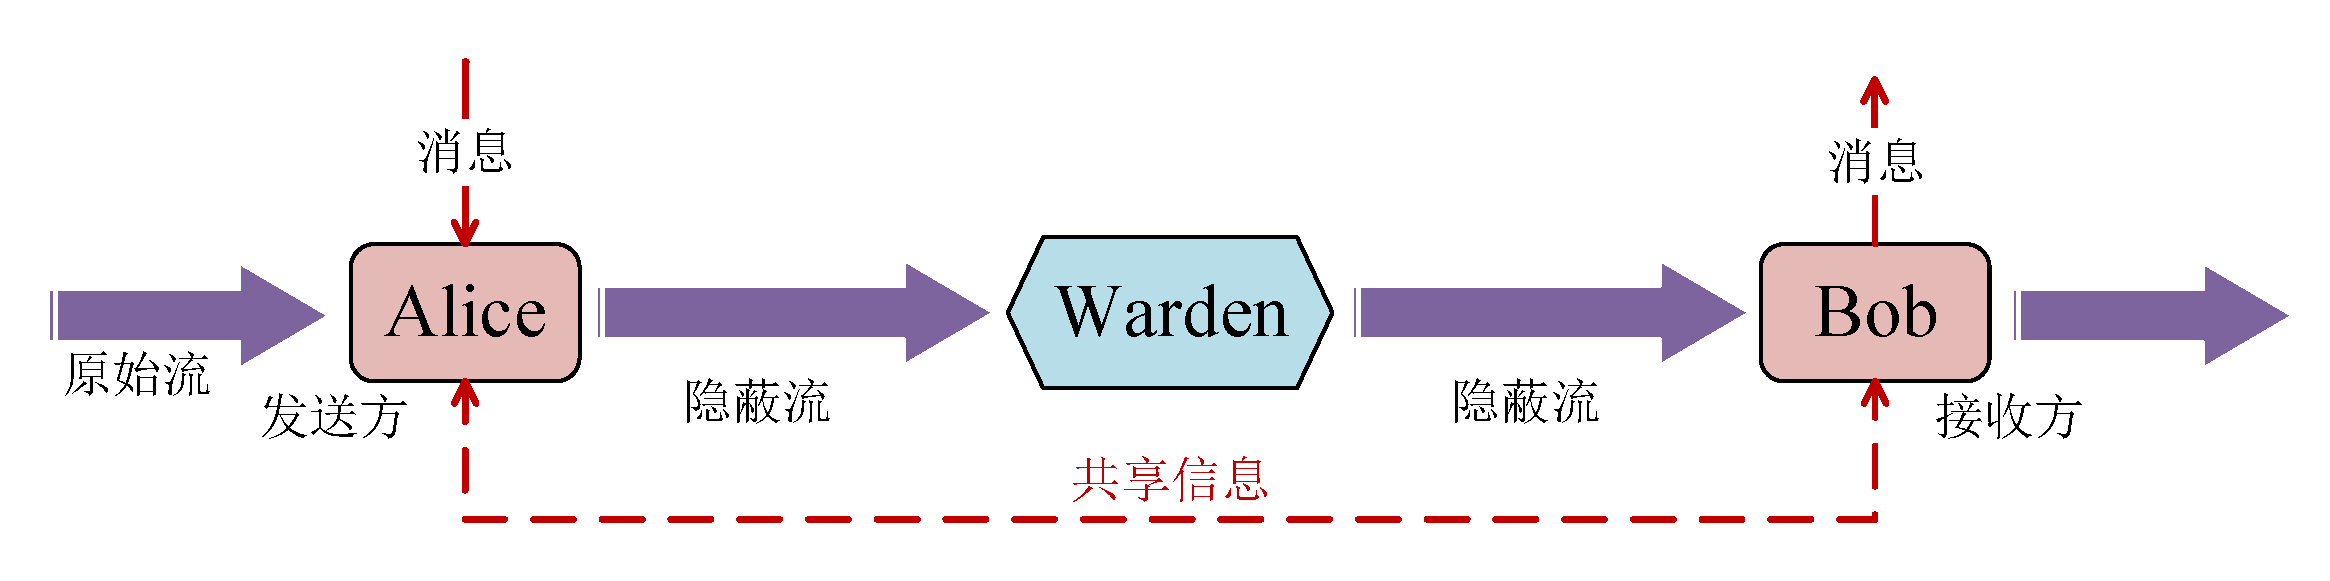
\includegraphics[width=\textwidth]{chapters/chapter1/figures/covert-channel.pdf}
        \caption{隐通道逻辑结构示意图}\label{fig:1:covert-channel}
	\end{figure}
}

对于隐通道的研究,主要集中在构建方法和检测方法两个方面。隐通道的逻辑结构示意如图\nref{fig:1:covert-channel},发送方和接收方利用共享信息,由发送方将宿主信道修改为隐蔽信道,接收方识别隐蔽信道中的特征信息,结合共享信息还原隐蔽消息。
隐通道最核心的环节,是如何实现调制过程,也就是将宿主信道修改为隐蔽信道的方式,这也是区分时间隐通道与存储隐通道的基本方法。
隐通道的检测方法,是针对特定类型的构建方法提出了,在应用范围上存在特定的局限性。
例如,基于IP(Internet Protocol)冗余字段的隐通道,修改了IP数据包头中的冗余字段,对宿主信道及上层应用不产生任何影响。对应的检测及消除措施,主要方式为扫描各字段的异常信息,并进行数据覆写,对部分存储隐通道实现有效防御。基于数据包顺序的隐通道,在构造过程中重新调整数据包序号,导致乱序现象出现,形成可检测的传输特征。通过数据包重排序,恢复正常顺序或再次打乱,在一定程度上进行消除。\nupcite{ahsan2002practical}

%时间隐通道相对存储隐通道的优势是什么
在不同的应用场景中,隐通道有多种表现形式。在单主机环境下,隐通道的构建可以利用磁盘响应时间,通过影响磁盘访问队列\nupcite{130771},实现单主机中不同进程之间的隐蔽传输;时间隐通道JitterBug捕获键盘输入中的敏感信息,并通过松耦合的网络隐通道进行传输,在SSH(Secure Shell)、VNC(Virtual Network Computing)及RDP(Remote Desktop Protocol)等远程访问场景中具有可操作性\nupcite{shah2006keyboards}。
在以太网环境中,存储隐通道的构建多基于网络协议,类似于音频、视频中常用的隐写术,待发送的消息块被嵌入到数据包中,如TCP(Transmission Control Protocol)包头中的冗余字段\nupcite{4317620}、IPv6包头中的AH及ESP字段\nupcite{10.1007/11767831_10};时间隐通道的构建,多基于数据包传输间隔及数据包发送顺序等。
相比于存储隐通道,时间隐通道在隐蔽性方面具有绝佳的优势,但受限于隐蔽信道的基础条件和网络噪声的影响,在传输能力及传输性能方面存在不足。因此,时间隐通道适用于少量核心消息的传输,存储隐通道适用于具有高性能传输需求的场景。

%移动互联网的兴起
随着第四代移动通信技术的广泛应用,以及移动智能终端的不断发展,移动互联网得到进一步发展,目前正在由4G时代过渡到5G时代\nupcite{7470940}。
第四代移动通信技术,也就是LTE(Long Term Evolution)技术,在接入带宽、空口时延及负载能力等方面均得到了提升,面向移动互联网的应用得到繁荣发展。
不同于原有的移动通信技术,LTE网络在设计中采用了全IP网络\nupcite{6398495}。网络中的所有数据均封装为IP数据包,实现了更高的数据转发能力及更低的传输延迟;对不同应用、不同类型数据包的优化及优先级调度,提供了更好的用户体验;传输网络的鲁棒性得到提升,不同应用场景下的适应能力得到提升。\nupcite{DBLP:journals/corr/abs-1810-02968}

%VoLTE是未来的趋势
由于LTE网络中取消了基于电路交换的通信技术,LTE网络中的语音通话必须向VoIP(Voice over IP)迁移,目前已经实现大规模商用。通过基于数据包交换的核心网传输方式,VoLTE在提供低延迟、高清晰度语音通话的同时,也支持低延迟的视频通话。
对于5G网络,音视频通话方案仍然会按照VoLTE的模式进行设计\nupcite{8412482},因此,对VoLTE的传输特征进行研究,并研究隐通道的存在基础及构建环境,符合技术发展趋势。
得益于LTE核心网的传输保证,VoLTE的通话质量要由于第三方VoIP方案。通过提高VoLTE数据包优先级,即使是高负载的网络环境中,通话延迟方面也具有显著优势;采用高效的编码方式,在平衡通话质量的同时,降低丢包率。\nupcite{anehill2012validating}

%研究VoLTE下时间隐通道构建方法,具有填补空白的意义
基于端到端的数据包传输,是VoLTE区别于VoIP应用的重要特征。通过减少数据包转发环节,VoLTE为时间隐通道的研究提供了新的环境,在VoLTE环境下,数据包的类型、传输顺序及网络抖动均存在较强的规律性,一定程度上破坏了时间隐通道的构建条件。研究基于主动丢包的时间隐通道方法,不仅扩充了VoLTE下隐通道的设计方法,对其它端到端传输环境也具有参考价值。
\section{国内外研究现状及难点}
\label{sec:intro:background}

本节说了什么

本节包含的内容

\subsection{基于移动互联网的时间隐通道}
\label{sec:intro:background:ctc}

在移动互联网环境下,构建时间隐通道,应当遵守怎样的约束

常用的构建方法

各种方法的总结,以及为何不能应用在VoLTE环境中

\subsection{时间隐通道的鲁棒性策略}
\label{sec:intro:background:robustness}

首先说明,时间隐通道因为自身的特性,在传输可靠性上,不如Overt Traffic

现有的时间隐通道方案,在保证鲁棒性反面,采用了怎样的手段,比如添加纠错信息、重传、特殊编码等

这些方法,对应用场景的限制及不足

\subsection{时间隐通道的检测方法}
\label{sec:intro:background:detect}

检测时间隐通道,通常从那几个要素方面进行考虑

检测判断,主要根据哪些因素来考量,包括分布、一致性

在该场景中,主要通过丢包的方法构建时间隐通道,所有,在现有的常用检测方法的基础上,还要对丢包的特征进行分析

%固定相只有物理交联结构的聚氨酯称为热塑性SMPU,而有化学交联结构称为热固性SMPU。热塑性和热固性形状记忆聚氨酯的形状记忆原理示意图如图\ref{fig:diagram}所示

%\begin{figure}
% \centering
% \includegraphics[width=0.75\textwidth]{chapters/chapter1/figures/figure1}
% \caption{热塑性形状记忆聚氨酯的形状记忆机理示意图}\label{fig:diagram}
%\end{figure}

%\begin{table}
%  \centering
%  \caption{水系聚氨酯分类} \label{tab:category}
%  \begin{tabular*}{0.9\textwidth}{@{\extracolsep{\fill}}cccc}
%  \toprule
%    类别			&水溶型		&胶体分散型		&乳液型 \\
%  \midrule
%    状态			&溶解$\sim$胶束	&分散		&白浊 \\
%    外观			&水溶型		&胶体分散型		&乳液型 \\
%    粒径$/\mu m$	&$<0.001$		&$0.001-0.1$		&$>0.1$ \\
%    重均分子量	&$1000\sim 10000$	&数千$\sim 20万$ &$>5000$ \\
%  \bottomrule
%  \end{tabular*}
%\end{table}

\section{研究内容及创新点}
\label{sec:intro:work}

\subsection{本文主要内容}
\label{sec:intro:work:mainwork}

随着VoLTE应用范围的不断扩大,研究在VoLTE环境下的时间隐通道构建方案,扩充了时间隐通道的构建方法,也进一步扩展对VoLTE音视频通话特征的研究。本文主要研究在VoLTE视频通话场景下,通过主动丢包的方式,构建鲁棒的时间隐通道。主要包括三个研究点,分别是VoLTE时间隐通道检测方法研究,基于Zigzag映射矩阵的时间隐通道构建方法研究,以及基于多重校验的时间隐通道构建方法研究。各部分之间的关联关系及研究指标如图\nref{fig:1:contents}。

\insertFigure{
	\begin{figure}
		\centering
        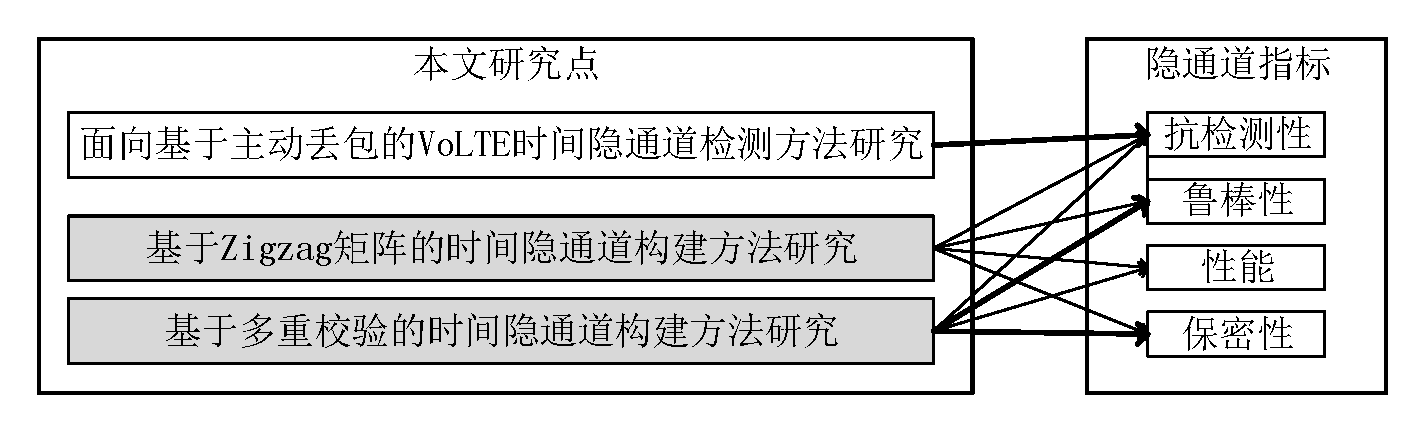
\includegraphics[width=0.75\textwidth]{chapters/chapter1/figures/struct.pdf}
        \caption{本文各研究点之间的关系}\label{fig:1:contents}
	\end{figure}
}

%背景介绍了什么
背景及相关工作部分,主要介绍了本论文主要工作的一些研究基础,以及国内外的研究现状。内容包括对VoLTE音视频传输方案的分析,分析了实际商用中VoLTE的数据产生、处理、传输、呈现流程,并分析了音视频在流程上的差异。对现有时间隐通道构造方案的分析,涵盖了以太网中的构造方案、移动互联网下的构造方案,以及有效的鲁棒性策略。通过分析VoLTE传输协议,研究丢包带来的影响,并充分利用协议中的随机字段,提高保密性。抗检测能力是时间隐通道的一个重要指标,通过研究现有的时间隐通道检测方法,针对该时间隐通道构建方法,选择可用的检测方法。

%检测方法介绍了什么
VoLTE时间隐通道检测方法研究,主要研究在VoLTE场景下,如何有效检测基于主动丢包的时间隐通道。为筛选有效的检测方法,首先对VoLTE通话抓包结果进行分析,由丢包率、IPD、突发丢包长度及丢包随机性几个方面分别展开。根据特征分析结果,提出了一组基于统计分析的时间隐通道检测方法,包含不同维度的多种检测方式。最后,通过模拟的方式,对这些方法进行模拟测试,判断是否具有显著效果。

%Zigzag方法说了什么
基于Zigzag映射矩阵的时间隐通道构建方法,研究利用Zigzag矩阵作为码字与符号关系的映射矩阵,并添加冗余校验信息,在抗检测性、鲁棒性及传输性能之间实现均衡。为了清楚地介绍该研究方法,按照研究背景、构造方法及实验结果及评估的顺序,对该方法的研究基础、架构设计、调制解调方法及实验测试结果分别进行介绍。经过实验测试证明,通过调整传输参数,该时间隐通道构建方法各方面结果良好。

%多重校验方法说了什么
基于多重校验的时间隐通道构建方法,重点研究如何进一步降低误码率,提高传输可靠性。在该时间隐通道方法中,设计了包括码字间校验、码字自校验以及符号校验三级校验模式,结合对连续丢包噪声具有抑制作用的映射矩阵,显著提高了传输鲁棒性,降低了误码率水平。该部分首先从研究背景基础开始,首先介绍该方法的设计架构,然后针对核心的鲁棒性鲁棒性方法逐层展开,最后进行实验测试与对比。实验结果表明,该时间隐通道的误码率水平较之前方案有了大幅度提升。

%以上各部分是怎样在逻辑上串起来的
背景及相关工作的介绍,分析出在VoLTE视频通话场景下,通过主动丢包的方式构建时间隐通道是可行的。与此同时,现有的检测方法及鲁棒性方法,无法有效覆盖这种隐通道构造模式。VoLTE时间隐通道检测方法研究,着重解决如何检测采用主动丢包的时间隐通道,同时也为接下来提出的构建方案提供检测依据。最后,两种不同的时间隐通道构建方法,分别从不同的方式,填补鲁棒性方面的构建需求,并通过实验进行验证。

\subsection{本文主要创新点}
\label{sec:intro:work:inno}

本文的研究重点,是在VoLTE场景下,通过主动丢包方式构建时间隐通道的方法,以及抗检测性评估方式。主要的创新点包括以下几点:

\begin{enumerate}
    \item 提出了一种VoLTE下时间隐通道检测方法,针对基于主动丢包的构建方法。该方法以统计分析为基础,综合多种量化评估方法,结合IPD及丢包特征两个维度进行检测判别。传统的时间隐通道检测方法,主要基于IPD分布特征进行检测识别,对基于主动丢包的时间隐通道来说,判别效果不够全面。本方法完善了时间隐通道的检测方式,经过实验测试,该时间隐通道检测方法有效可行。
    \item 提出了一种基于Zigzag映射矩阵的时间隐通道构建方法,该方法的核心,是隐通道的编码及调制过程,在编码过程中添加CRC校验信息,利用Zigzag矩阵完成码字到符号的转换,最后添加随机偏移量得到要丢弃的数据包序号。该方法以简单高效的方式,以轻量级校验模式,在保证传输性能的同时,降低计算复杂度保证鲁棒性,适用于容许一定误码率的应用场景。
    \item 提出了一种基于多重校验的时间隐通道构造方法,重点研究如何通过逐级校验的方式,降低噪声对时间隐通道的干扰,提高噪声干扰下的鲁棒性。该方法的核心,是在不同的处理阶段引入相互独立的校验方式,在解调过程中逐级剔除噪声干扰,还原概率最高的隐蔽消息。此外,通过引入可调映射矩阵,将连续丢包事件分散到多个组,减小每组的噪声强度,降低误码率水平。
\end{enumerate}

\subsection{本文组织结构}
\label{sec:intro:work:struct}

全文共分五章,文章的组织结构如下:
\begin{itemize}
    \item 第1章,对本文的研究领域及主要内容进行介绍
    \item 第2章,本文中涉及到的研究背景,及国内外相关工作的介绍。包含当前研究工作的基础介绍,当前隐通道构建及检测方面的研究成果,以及时间隐通道应当满足的基本要求。
    \item 第3章,介绍VoLTE下时间隐通道检测方法,结合当前成熟的检测方法,在IPD检测的基础上,添加对丢包特征统计的检测。监测维度涵盖了基于统计曲线的检测、基于熵的检测及基于相对距离的检测方法,能够对基于主动丢包的时间隐通道进行有效识别。该检测方法,也是本文两种时间隐通道构建方法抗检测能力的评估参照。
    \item 第4章,介绍基于Zigzag映射矩阵的时间隐通道构建方法,由研究背景开始,首先介绍构建方法的设计方案,然后通过实验,对隐通道的各项指标进行评估。
    \item 第5章,介绍基于多重校验的时间隐通道构建方法,首先对方法背景进行介绍,然后对时间隐通道的整体流程进行展开,接下来对关键的鲁棒性方案设计逐级展开分析,最后分析实验结果及指标。
\end{itemize}

%%%%%%%%%%%%%论文正文部分%%%%%%%%%%%%%%%%%%%%%%%%%%%%%%%%%%%%%%%%
\chapter{引言}
\label{chap:intro}
%在下方加入各小节内容
\section{研究背景和意义}
\label{sec:intro:backgroud}

%介绍什么是隐通道

%传统的时间隐通道,是利用数据的时间变化特性,承载目标数据。例如基于IP的时间隐通道(IP-CTC)[3].,基于回复时间的隐通道(TR-CTC)[4].,基于IPD的时间隐通道(IPD-CTC),利用数据包的长度变化规律来传送数据[10].,利用数据包之间的时间间隔(IPD)传送数据[12].,或者基于数据包分类的时间隐通道[13].,以及基于模型的时间隐通道(MB-CTC)[11].。

隐通道的明确定义,由Lampson在1973年提出\nupcite{4317620},隐通道能够打破系统中的安全限制,实现消息在不同安全级别之间的隐蔽传输。隐通道的存在意义,是在传输信道被监听的前提下,实现数据传输过程,并且监听者无法察觉传输过程。监听者通常对数据内容及传输过程进行监控,只允许传输符合规则的数据,拦截其它的会话请求。研究VoLTE中的时间隐通道构建方法,解决当双方只被允许进行VoLTE通话时,数据隐蔽、鲁棒传输的需求。

经过研究探索,随着互联网应用范围的扩大,网络应用逐渐丰富,隐通道的应用环境由传统的单主机平台,扩展到各种类型的网络设备之中。
隐通道的实现方式多种多样,根据构建方式的差异,隐通道通常被划分为时间隐通道及存储隐通道两种类型,存储隐通道依赖于双方对相同存储位置的读写访问,时间隐通道依赖于双方对时间特征的识别。\nupcite{1702197}
随着移动互联网的不断扩展,隐通道为终端之间的安全隐蔽传输,提供了可行的解决方案,满足了特定需求场景下的传输需求。\nupcite{6542541}

\insertFigure{
	\begin{figure}
	    \centering
        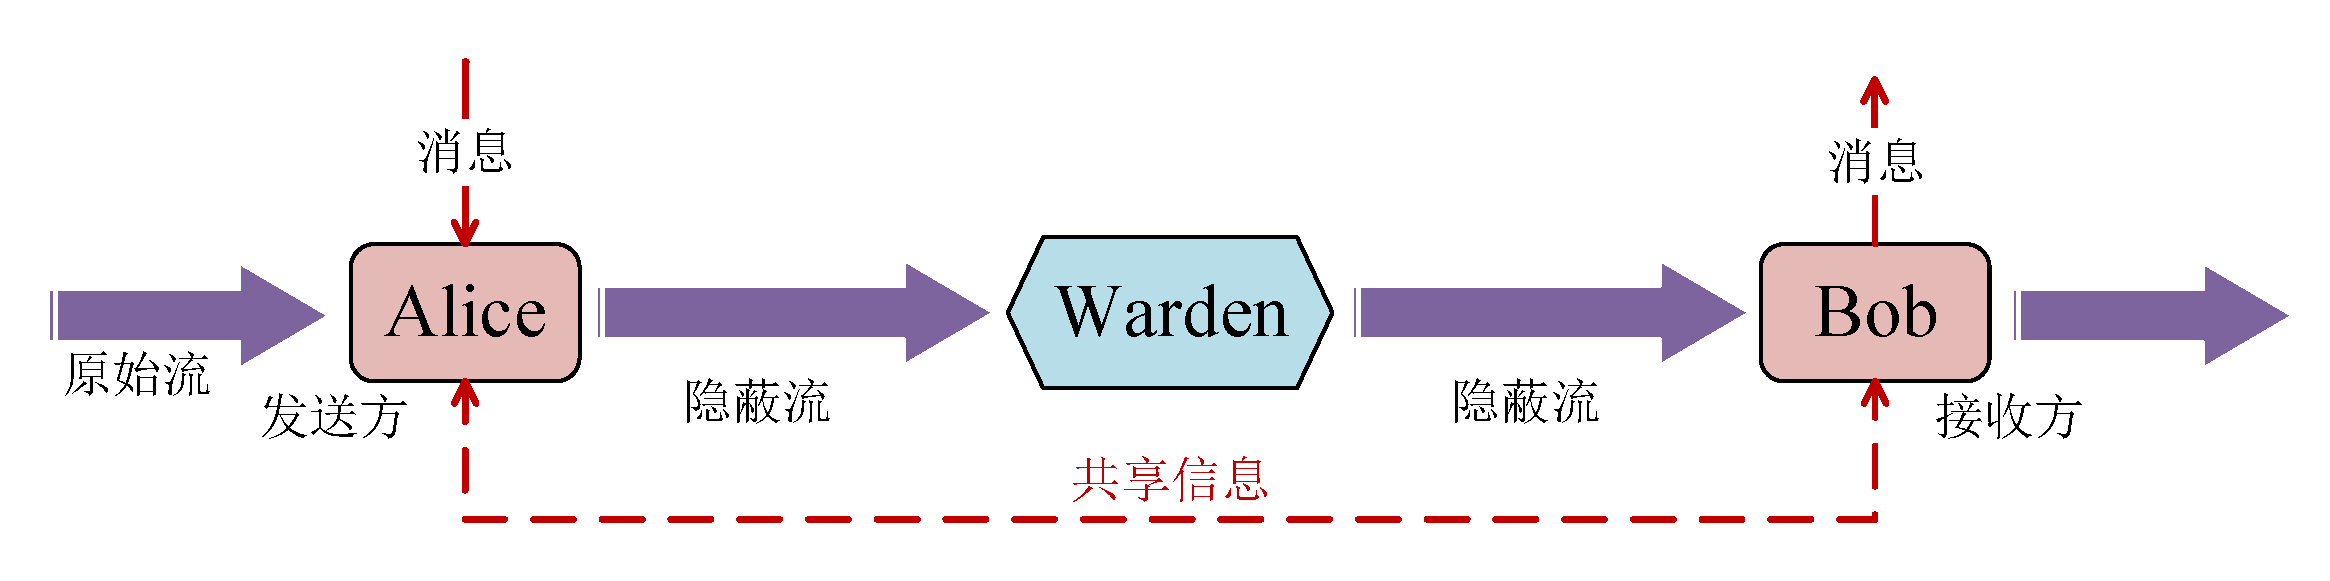
\includegraphics[width=\textwidth]{chapters/chapter1/figures/covert-channel.pdf}
        \caption{隐通道逻辑结构示意图}\label{fig:1:covert-channel}
	\end{figure}
}

对于隐通道的研究,主要集中在构建方法和检测方法两个方面。隐通道的逻辑结构示意如图\nref{fig:1:covert-channel},发送方和接收方利用共享信息,由发送方将宿主信道修改为隐蔽信道,接收方识别隐蔽信道中的特征信息,结合共享信息还原隐蔽消息。
隐通道最核心的环节,是如何实现调制过程,也就是将宿主信道修改为隐蔽信道的方式,这也是区分时间隐通道与存储隐通道的基本方法。
隐通道的检测方法,是针对特定类型的构建方法提出了,在应用范围上存在特定的局限性。
例如,基于IP(Internet Protocol)冗余字段的隐通道,修改了IP数据包头中的冗余字段,对宿主信道及上层应用不产生任何影响。对应的检测及消除措施,主要方式为扫描各字段的异常信息,并进行数据覆写,对部分存储隐通道实现有效防御。基于数据包顺序的隐通道,在构造过程中重新调整数据包序号,导致乱序现象出现,形成可检测的传输特征。通过数据包重排序,恢复正常顺序或再次打乱,在一定程度上进行消除。\nupcite{ahsan2002practical}

%时间隐通道相对存储隐通道的优势是什么
在不同的应用场景中,隐通道有多种表现形式。在单主机环境下,隐通道的构建可以利用磁盘响应时间,通过影响磁盘访问队列\nupcite{130771},实现单主机中不同进程之间的隐蔽传输;时间隐通道JitterBug捕获键盘输入中的敏感信息,并通过松耦合的网络隐通道进行传输,在SSH(Secure Shell)、VNC(Virtual Network Computing)及RDP(Remote Desktop Protocol)等远程访问场景中具有可操作性\nupcite{shah2006keyboards}。
在以太网环境中,存储隐通道的构建多基于网络协议,类似于音频、视频中常用的隐写术,待发送的消息块被嵌入到数据包中,如TCP(Transmission Control Protocol)包头中的冗余字段\nupcite{4317620}、IPv6包头中的AH及ESP字段\nupcite{10.1007/11767831_10};时间隐通道的构建,多基于数据包传输间隔及数据包发送顺序等。
相比于存储隐通道,时间隐通道在隐蔽性方面具有绝佳的优势,但受限于隐蔽信道的基础条件和网络噪声的影响,在传输能力及传输性能方面存在不足。因此,时间隐通道适用于少量核心消息的传输,存储隐通道适用于具有高性能传输需求的场景。

%移动互联网的兴起
随着第四代移动通信技术的广泛应用,以及移动智能终端的不断发展,移动互联网得到进一步发展,目前正在由4G时代过渡到5G时代\nupcite{7470940}。
第四代移动通信技术,也就是LTE(Long Term Evolution)技术,在接入带宽、空口时延及负载能力等方面均得到了提升,面向移动互联网的应用得到繁荣发展。
不同于原有的移动通信技术,LTE网络在设计中采用了全IP网络\nupcite{6398495}。网络中的所有数据均封装为IP数据包,实现了更高的数据转发能力及更低的传输延迟;对不同应用、不同类型数据包的优化及优先级调度,提供了更好的用户体验;传输网络的鲁棒性得到提升,不同应用场景下的适应能力得到提升。\nupcite{DBLP:journals/corr/abs-1810-02968}

%VoLTE是未来的趋势
由于LTE网络中取消了基于电路交换的通信技术,LTE网络中的语音通话必须向VoIP(Voice over IP)迁移,目前已经实现大规模商用。通过基于数据包交换的核心网传输方式,VoLTE在提供低延迟、高清晰度语音通话的同时,也支持低延迟的视频通话。
对于5G网络,音视频通话方案仍然会按照VoLTE的模式进行设计\nupcite{8412482},因此,对VoLTE的传输特征进行研究,并研究隐通道的存在基础及构建环境,符合技术发展趋势。
得益于LTE核心网的传输保证,VoLTE的通话质量要由于第三方VoIP方案。通过提高VoLTE数据包优先级,即使是高负载的网络环境中,通话延迟方面也具有显著优势;采用高效的编码方式,在平衡通话质量的同时,降低丢包率。\nupcite{anehill2012validating}

%研究VoLTE下时间隐通道构建方法,具有填补空白的意义
基于端到端的数据包传输,是VoLTE区别于VoIP应用的重要特征。通过减少数据包转发环节,VoLTE为时间隐通道的研究提供了新的环境,在VoLTE环境下,数据包的类型、传输顺序及网络抖动均存在较强的规律性,一定程度上破坏了时间隐通道的构建条件。研究基于主动丢包的时间隐通道方法,不仅扩充了VoLTE下隐通道的设计方法,对其它端到端传输环境也具有参考价值。
\section{国内外研究现状及难点}
\label{sec:intro:background}

本节说了什么

本节包含的内容

\subsection{基于移动互联网的时间隐通道}
\label{sec:intro:background:ctc}

在移动互联网环境下,构建时间隐通道,应当遵守怎样的约束

常用的构建方法

各种方法的总结,以及为何不能应用在VoLTE环境中

\subsection{时间隐通道的鲁棒性策略}
\label{sec:intro:background:robustness}

首先说明,时间隐通道因为自身的特性,在传输可靠性上,不如Overt Traffic

现有的时间隐通道方案,在保证鲁棒性反面,采用了怎样的手段,比如添加纠错信息、重传、特殊编码等

这些方法,对应用场景的限制及不足

\subsection{时间隐通道的检测方法}
\label{sec:intro:background:detect}

检测时间隐通道,通常从那几个要素方面进行考虑

检测判断,主要根据哪些因素来考量,包括分布、一致性

在该场景中,主要通过丢包的方法构建时间隐通道,所有,在现有的常用检测方法的基础上,还要对丢包的特征进行分析

%固定相只有物理交联结构的聚氨酯称为热塑性SMPU,而有化学交联结构称为热固性SMPU。热塑性和热固性形状记忆聚氨酯的形状记忆原理示意图如图\ref{fig:diagram}所示

%\begin{figure}
% \centering
% \includegraphics[width=0.75\textwidth]{chapters/chapter1/figures/figure1}
% \caption{热塑性形状记忆聚氨酯的形状记忆机理示意图}\label{fig:diagram}
%\end{figure}

%\begin{table}
%  \centering
%  \caption{水系聚氨酯分类} \label{tab:category}
%  \begin{tabular*}{0.9\textwidth}{@{\extracolsep{\fill}}cccc}
%  \toprule
%    类别			&水溶型		&胶体分散型		&乳液型 \\
%  \midrule
%    状态			&溶解$\sim$胶束	&分散		&白浊 \\
%    外观			&水溶型		&胶体分散型		&乳液型 \\
%    粒径$/\mu m$	&$<0.001$		&$0.001-0.1$		&$>0.1$ \\
%    重均分子量	&$1000\sim 10000$	&数千$\sim 20万$ &$>5000$ \\
%  \bottomrule
%  \end{tabular*}
%\end{table}

\section{研究内容及创新点}
\label{sec:intro:work}

\subsection{本文主要内容}
\label{sec:intro:work:mainwork}

随着VoLTE应用范围的不断扩大,研究在VoLTE环境下的时间隐通道构建方案,扩充了时间隐通道的构建方法,也进一步扩展对VoLTE音视频通话特征的研究。本文主要研究在VoLTE视频通话场景下,通过主动丢包的方式,构建鲁棒的时间隐通道。主要包括三个研究点,分别是VoLTE时间隐通道检测方法研究,基于Zigzag映射矩阵的时间隐通道构建方法研究,以及基于多重校验的时间隐通道构建方法研究。各部分之间的关联关系及研究指标如图\nref{fig:1:contents}。

\insertFigure{
	\begin{figure}
		\centering
        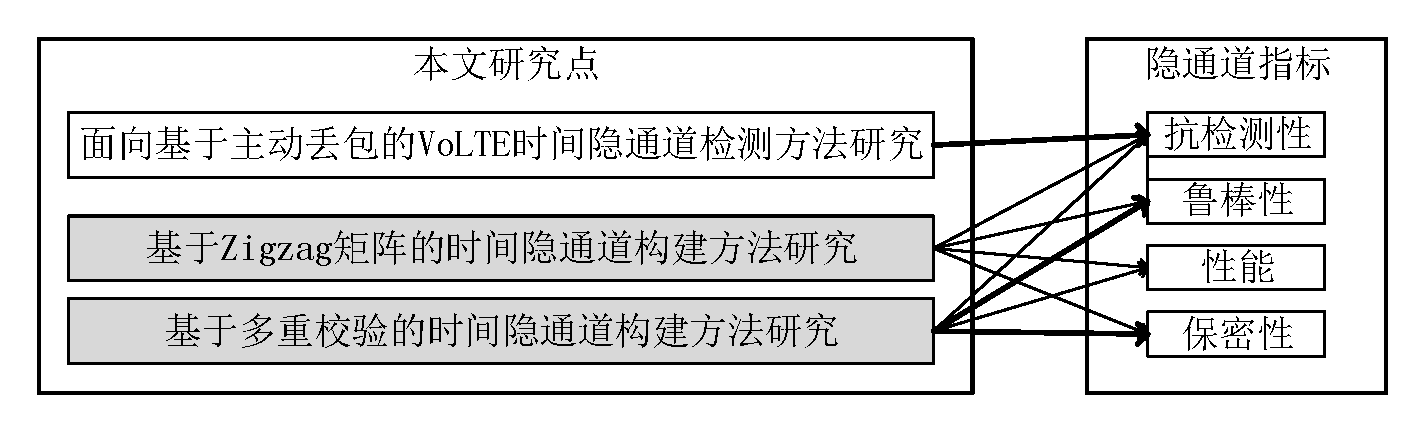
\includegraphics[width=0.75\textwidth]{chapters/chapter1/figures/struct.pdf}
        \caption{本文各研究点之间的关系}\label{fig:1:contents}
	\end{figure}
}

%背景介绍了什么
背景及相关工作部分,主要介绍了本论文主要工作的一些研究基础,以及国内外的研究现状。内容包括对VoLTE音视频传输方案的分析,分析了实际商用中VoLTE的数据产生、处理、传输、呈现流程,并分析了音视频在流程上的差异。对现有时间隐通道构造方案的分析,涵盖了以太网中的构造方案、移动互联网下的构造方案,以及有效的鲁棒性策略。通过分析VoLTE传输协议,研究丢包带来的影响,并充分利用协议中的随机字段,提高保密性。抗检测能力是时间隐通道的一个重要指标,通过研究现有的时间隐通道检测方法,针对该时间隐通道构建方法,选择可用的检测方法。

%检测方法介绍了什么
VoLTE时间隐通道检测方法研究,主要研究在VoLTE场景下,如何有效检测基于主动丢包的时间隐通道。为筛选有效的检测方法,首先对VoLTE通话抓包结果进行分析,由丢包率、IPD、突发丢包长度及丢包随机性几个方面分别展开。根据特征分析结果,提出了一组基于统计分析的时间隐通道检测方法,包含不同维度的多种检测方式。最后,通过模拟的方式,对这些方法进行模拟测试,判断是否具有显著效果。

%Zigzag方法说了什么
基于Zigzag映射矩阵的时间隐通道构建方法,研究利用Zigzag矩阵作为码字与符号关系的映射矩阵,并添加冗余校验信息,在抗检测性、鲁棒性及传输性能之间实现均衡。为了清楚地介绍该研究方法,按照研究背景、构造方法及实验结果及评估的顺序,对该方法的研究基础、架构设计、调制解调方法及实验测试结果分别进行介绍。经过实验测试证明,通过调整传输参数,该时间隐通道构建方法各方面结果良好。

%多重校验方法说了什么
基于多重校验的时间隐通道构建方法,重点研究如何进一步降低误码率,提高传输可靠性。在该时间隐通道方法中,设计了包括码字间校验、码字自校验以及符号校验三级校验模式,结合对连续丢包噪声具有抑制作用的映射矩阵,显著提高了传输鲁棒性,降低了误码率水平。该部分首先从研究背景基础开始,首先介绍该方法的设计架构,然后针对核心的鲁棒性鲁棒性方法逐层展开,最后进行实验测试与对比。实验结果表明,该时间隐通道的误码率水平较之前方案有了大幅度提升。

%以上各部分是怎样在逻辑上串起来的
背景及相关工作的介绍,分析出在VoLTE视频通话场景下,通过主动丢包的方式构建时间隐通道是可行的。与此同时,现有的检测方法及鲁棒性方法,无法有效覆盖这种隐通道构造模式。VoLTE时间隐通道检测方法研究,着重解决如何检测采用主动丢包的时间隐通道,同时也为接下来提出的构建方案提供检测依据。最后,两种不同的时间隐通道构建方法,分别从不同的方式,填补鲁棒性方面的构建需求,并通过实验进行验证。

\subsection{本文主要创新点}
\label{sec:intro:work:inno}

本文的研究重点,是在VoLTE场景下,通过主动丢包方式构建时间隐通道的方法,以及抗检测性评估方式。主要的创新点包括以下几点:

\begin{enumerate}
    \item 提出了一种VoLTE下时间隐通道检测方法,针对基于主动丢包的构建方法。该方法以统计分析为基础,综合多种量化评估方法,结合IPD及丢包特征两个维度进行检测判别。传统的时间隐通道检测方法,主要基于IPD分布特征进行检测识别,对基于主动丢包的时间隐通道来说,判别效果不够全面。本方法完善了时间隐通道的检测方式,经过实验测试,该时间隐通道检测方法有效可行。
    \item 提出了一种基于Zigzag映射矩阵的时间隐通道构建方法,该方法的核心,是隐通道的编码及调制过程,在编码过程中添加CRC校验信息,利用Zigzag矩阵完成码字到符号的转换,最后添加随机偏移量得到要丢弃的数据包序号。该方法以简单高效的方式,以轻量级校验模式,在保证传输性能的同时,降低计算复杂度保证鲁棒性,适用于容许一定误码率的应用场景。
    \item 提出了一种基于多重校验的时间隐通道构造方法,重点研究如何通过逐级校验的方式,降低噪声对时间隐通道的干扰,提高噪声干扰下的鲁棒性。该方法的核心,是在不同的处理阶段引入相互独立的校验方式,在解调过程中逐级剔除噪声干扰,还原概率最高的隐蔽消息。此外,通过引入可调映射矩阵,将连续丢包事件分散到多个组,减小每组的噪声强度,降低误码率水平。
\end{enumerate}

\subsection{本文组织结构}
\label{sec:intro:work:struct}

全文共分五章,文章的组织结构如下:
\begin{itemize}
    \item 第1章,对本文的研究领域及主要内容进行介绍
    \item 第2章,本文中涉及到的研究背景,及国内外相关工作的介绍。包含当前研究工作的基础介绍,当前隐通道构建及检测方面的研究成果,以及时间隐通道应当满足的基本要求。
    \item 第3章,介绍VoLTE下时间隐通道检测方法,结合当前成熟的检测方法,在IPD检测的基础上,添加对丢包特征统计的检测。监测维度涵盖了基于统计曲线的检测、基于熵的检测及基于相对距离的检测方法,能够对基于主动丢包的时间隐通道进行有效识别。该检测方法,也是本文两种时间隐通道构建方法抗检测能力的评估参照。
    \item 第4章,介绍基于Zigzag映射矩阵的时间隐通道构建方法,由研究背景开始,首先介绍构建方法的设计方案,然后通过实验,对隐通道的各项指标进行评估。
    \item 第5章,介绍基于多重校验的时间隐通道构建方法,首先对方法背景进行介绍,然后对时间隐通道的整体流程进行展开,接下来对关键的鲁棒性方案设计逐级展开分析,最后分析实验结果及指标。
\end{itemize}
%%==================================================
%% chapter02.tex for BIT Master Thesis
%% modified by yang yating
%% version: 0.1
%% last update: Dec 25th, 2016
%%==================================================
\chapter{背景及相关工作}
\label{chap:backinfo}

本章主要介绍,关于……的背景

及国内外相关工作的概述

%在下方加入各小节内容
\section{VoLTE音视频传输方案}
\label{chap:backinfo:volte}

%VoLTE实现概述

\insertFigure{
	\begin{figure}[htbp]
		\centering
        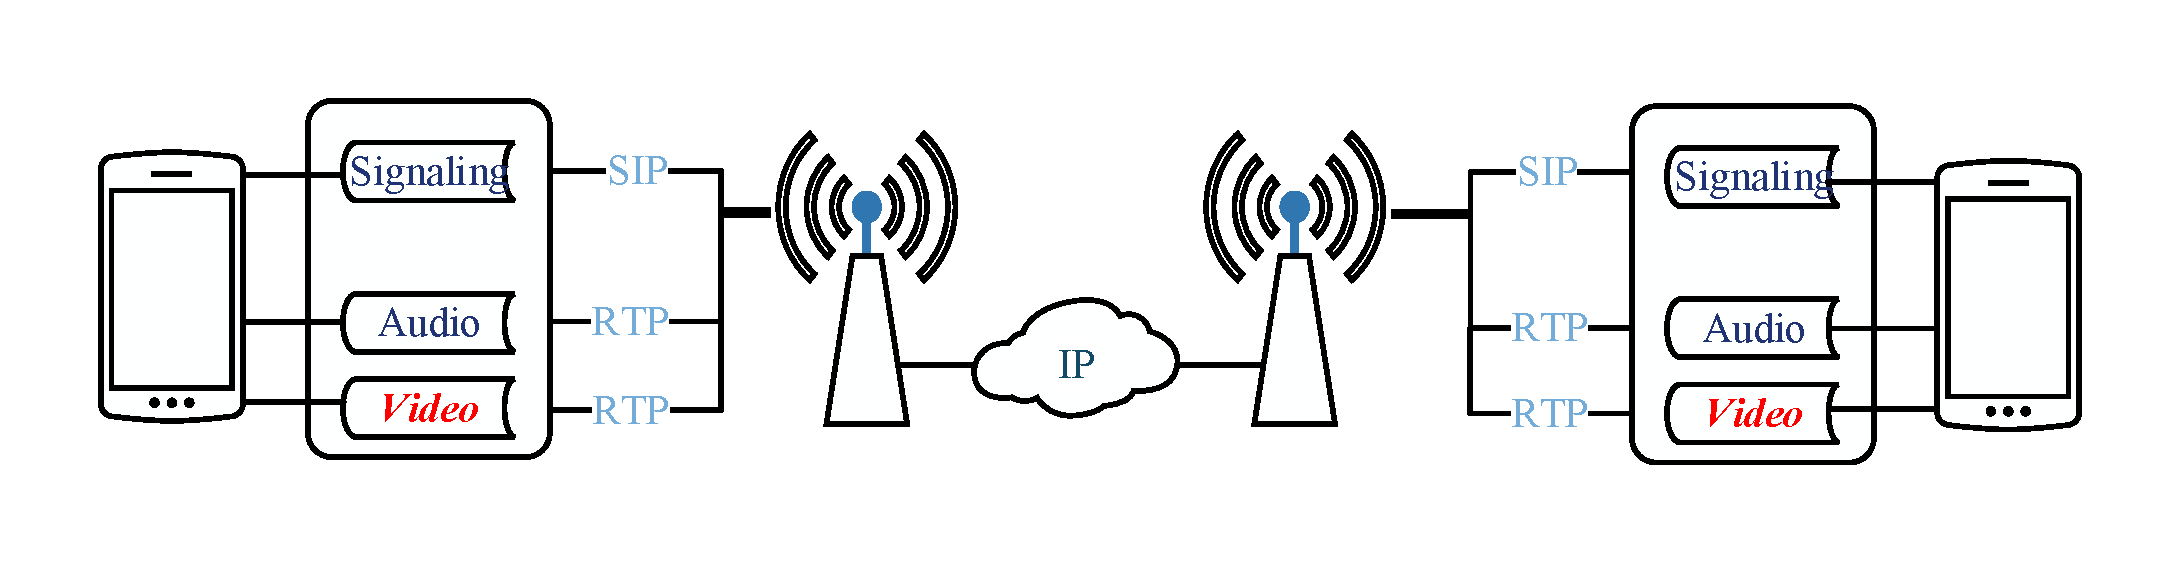
\includegraphics[width=0.95\textwidth]{chapters/chapter2/figures/volte-model.pdf}
        \caption{VoLTE视频通话中的数据流}\label{fig:2:volte-model}
	\end{figure}
}

语音通信功能是移动通信技术的基本需求,随着智能终端的发展,用户的移动数据需求才逐渐占据主流。在移动通信标准中,基于LTE的第四代移动通信技术已经转变为全IP网络,实现了语音主导到数据主导的转换。不同于原有的通信方案,LTE对数据传输进行了优化,同时对音视频通话功能进行了升级。

\subsection{VoLTE数据处理流程}
\label{chap:backinfo:volte:datastream}

在2G及3G时代,基于电路交换音频通话技术,是支撑语音业务的核心解决方案。进入4G时代,核心网络改变为全数据包交换,基于电路交换的音频通话已经无法兼容,需要全新的通话模式。于是,类似于VoIP音视频解决方案,基于LTE的VoLTE成为4G时代的音视频通话方案。在实际应用中,支持VoLTE的终端能够快速建立呼叫,否则将回落到3G或2G网络,从而兼容多种设备及场景。\nupcite{poikselka2012voice}

如图\nref{fig:2:volte-model},VoLTE视频通话过程中,需要三个数据信道,分别为信令信道、语音信道及视频信道,所有的信道均采用数据包进行传输。通过音视频分离方式,VoLTE实现了多场景兼容。通过信令信道,对通话模式及参数进行协商,决定语音信道及视频信道采用的编码方式。相对2G及3G网络,LTE支持的数据上行速率有了显著提升,能够支撑更多的终端进行高清晰度通话。\nupcite{ZHANG201929}

\insertTable{
    \begin{table}[htbp]
        \centering
        \caption{LTE业务QCI分配表概述}
        \label{tab:2:qci-classification}
        \begin{threeparttable}
            \begin{tabular*}{\textwidth}{@{\extracolsep{\fill}}cccccc}
                \toprule
                QCI\tnote{1}分类 & 资源类型 & 优先级 & 可接受延迟 & 可接受丢包率 & 服务类型 \\ 
                \midrule
                1 & 保证QoS\tnote{2} & 2 & 100 ms & $10^{-2}$ & VoLTE语音 \\ 
                2 & 保证QoS & 4 & 150 ms & $10^{-3}$ & VoLTE视频 \\
                5 & 不保证QoS & 1 & 100 ms & $10^{-6}$ & VoLTE信令 \\
                7 & 不保证QoS & 7 & 100 ms & $10^{-6}$ & 交互式音视频应用 \\
                \bottomrule
            \end{tabular*}
            \begin{tablenotes}
                \footnotesize
                \item[1] QCI指Quality of Service Class Identifiers,QoS分类标签
                \item[2] QoS指Quality of Service,服务质量
            \end{tablenotes}
        \end{threeparttable}
    \end{table}
}

相较于固网,移动无线网络受噪声干扰明显,导致用户通话体验变差。如表\nref{tab:2:qci-classification},根据LTE业务分类,VoLTE的信令数据包具有1级最高优先级,可接受时延为{100\ ms},可接受丢包率为$10^{-6}$;VoLTE语音数据包具有2级优先级,可接受时延为{100\ ms},可接受丢包率为$10^{-2}$;VoLTE视频数据包优先级降为4级,可接受时延为{150\ ms},可接受丢包率为$10^{-3}$。另一方面,即使VoIP应用的数据包也是经LTE网络传输,其服务质量也是完全不同的,运营商网络只保证尽力传输。VoIP应用的音视频数据对应的优先级为7,可接受时延为{100\ ms},可接受丢包率为$10^{-6}$。\nupcite{7154042,6996582,Li:2015:IVS:2810103.2813618}

因此,VoLTE相较于其它VoIP应用,受网络调度产生抖动的几率要小。时间隐通道的操作空间较小,对构建方法提出了新的挑战。

\subsection{VoLTE数据包传输特征}
\label{chap:backinfo:volte:packets}
%VoLTE音视频分流处理的模式(分清楚执行组件),结合传输的逻辑设计
通过支持VoLTE的终端设备进行视频通话,参与数据处理的处理器通常由两部分组成。其中一个是AP(Application Processor)也就是应用处理器,另外一个是BP(Baseband Processor)也就是基带处理器。AP参与操作系统中通用数据的处理,BP负责的是无线通信数据的处理,二者相互补充,共同完成智能终端设备的数据处理任务。

\insertFigure{
	\begin{figure}[htbp]
		\centering
        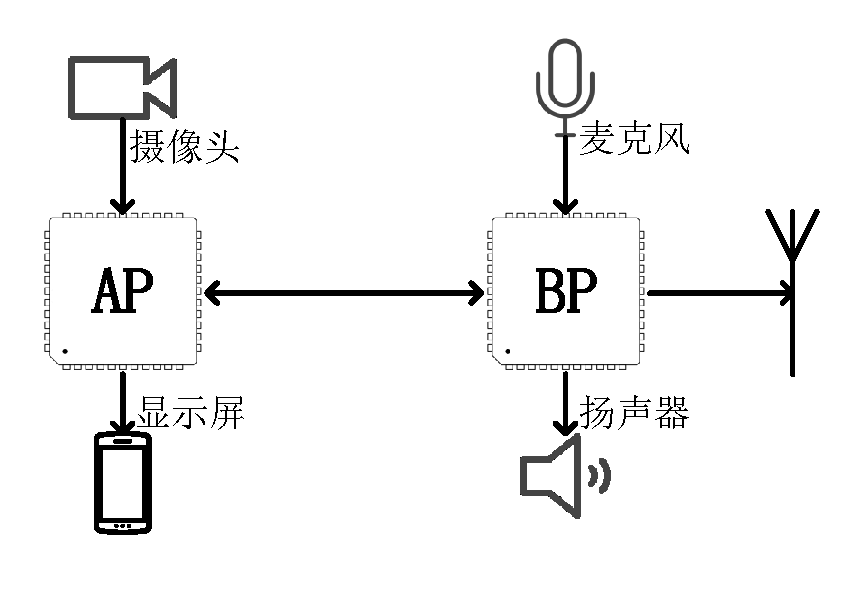
\includegraphics[width=0.55\textwidth]{chapters/chapter2/figures/ap-bp.pdf}
        \caption{VoLTE视频通话时AP与BP功能划分}\label{fig:2:ap-bp}
	\end{figure}
}

如图\nref{fig:2:ap-bp},AP与BP对应不同的媒体类型。对于VoLTE语音数据,由基带处理器按照设定的时间间隔,完成模拟信号的采样、编码,并将打包好的语音数据包通过射频系统传输。对于VoLTE视频数据,由于图像处理模块集成在应用处理器中,视频数据包需要应用处理器参与。应用处理器调用摄像系统驱动,获取编码后的视频数据流,按照视频帧分别进行切片打包,得到RTP视频数据包。视频数据包由系统内核中的协议栈发送,最终由BP通过射频系统传输。类似的,在接收阶段,VoLTE语音数据由基带处理器完成接收、解包、解码,并交由扬声器进行播放。VoLTE视频数据包则交付系统中的网络组件,完成解包、解码后,由通话软件显示在屏幕上。\nupcite{ZHANG201929,guo2019volte}

%抓包结果,分析传输特征,时间间隔、发送密度
\subsubsection{音视频数据包发送特征}
\label{chap:backinfo:volte:packets:send}

\insertFigure{
    \begin{figure}[htbp]
        \centering
        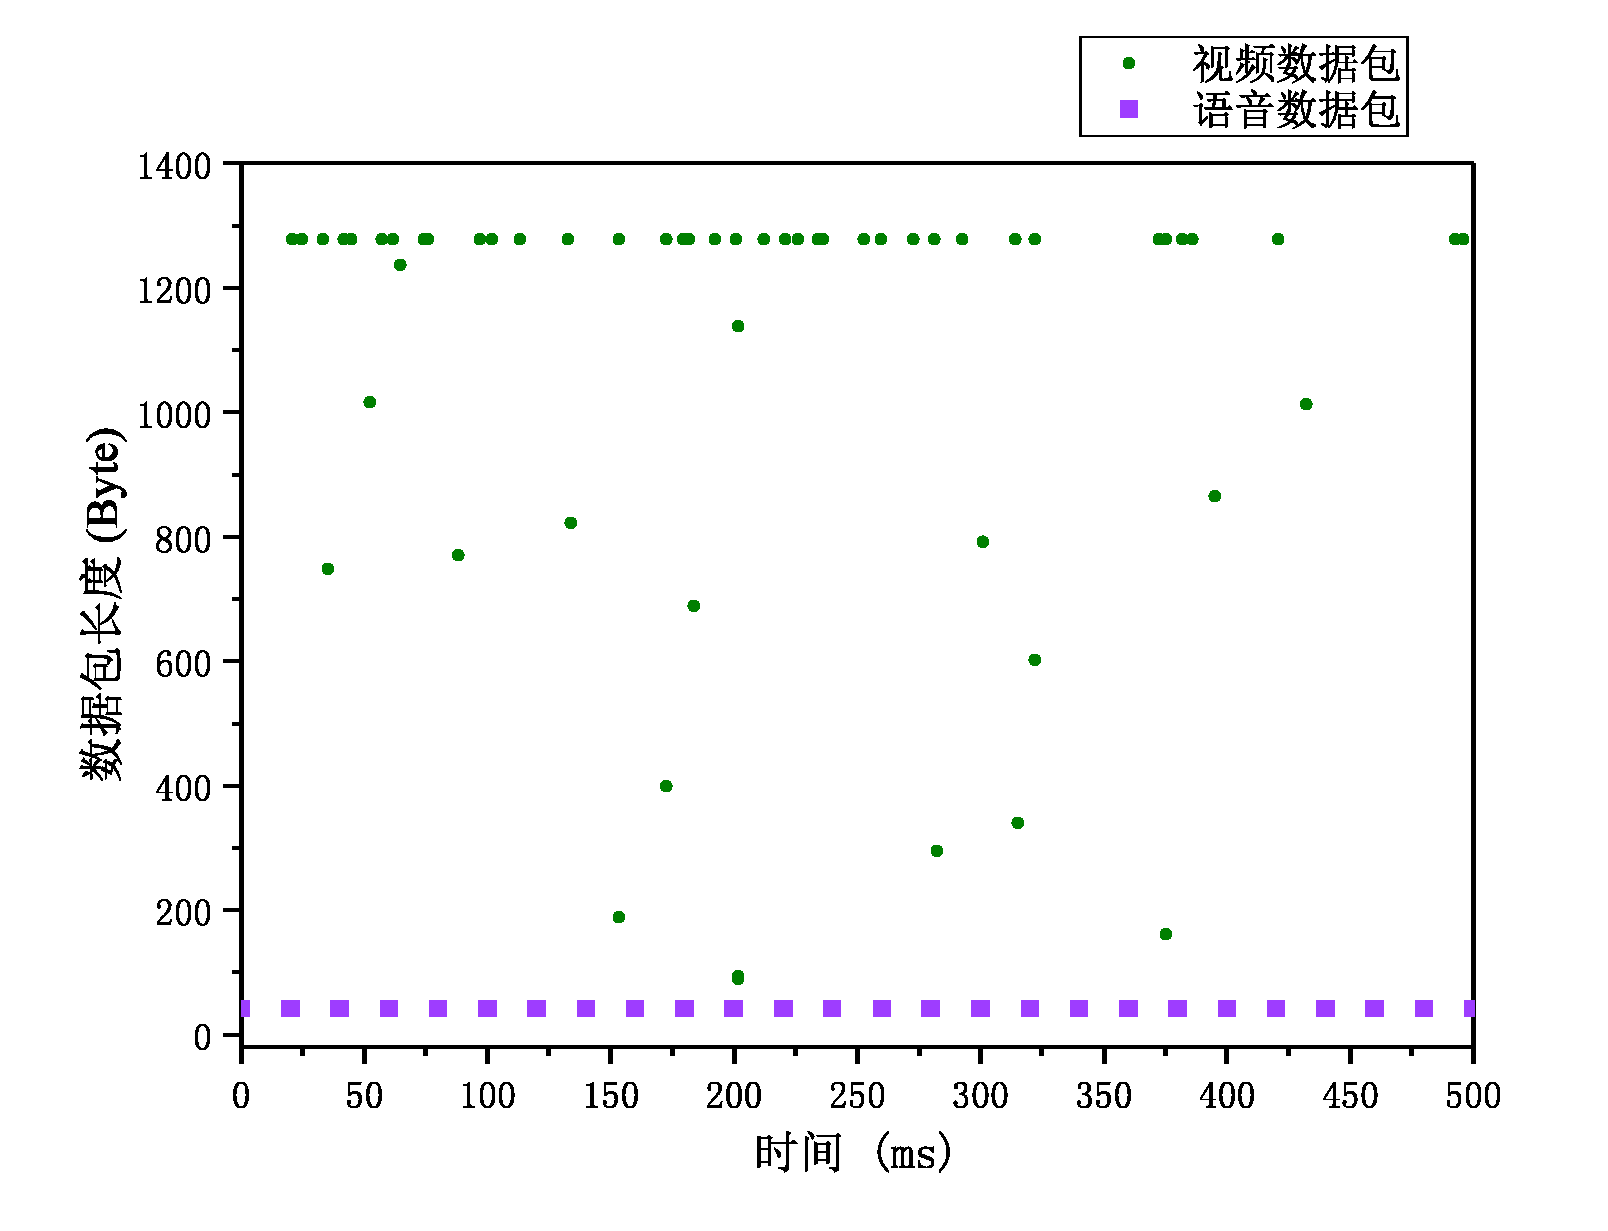
\includegraphics[width=0.75\textwidth]{chapters/chapter2/figures/length-audio-video.pdf}
        \caption{VoLTE音视频数据包发送间隔示意}\label{fig:2:audio-video}
    \end{figure}
}

对于音频数据包,采用AMR-WB(Adaptive Multi-Rate Wideband)格式编码时,数据包在非静音期每{20\ ms}发送一次,在静音期不发送数据包。\nupcite{8288828}对于视频数据包,数据包发送间隔取决于视频刷新率及编码结果,具有很大的不确定性。\nupcite{zhang2019timestamp}如图\nref{fig:2:audio-video},VoLTE视频数据包的长度虽然在{1300\ 字节}左右有集中分布,但仍有部分数据包长度随机变化;另一方面,VoLTE语音数据包的发送间隔具有规律性,相比较视频数据包的聚集现象更普遍。

\subsubsection{视频数据包发送与接收IPD分布特征}
\label{chap:backinfo:volte:packets:ipd}
如本文\nref{chap:backinfo:volte:packets:send}所述,VoLTE语音数据包的IPD规律性明显,对构建时间隐通道不利。研究VoLTE视频数据包的传输特征,对VoLTE下时间隐通道构造方法的研究具有重要意义,VoLTE视频数据流对噪声敏感度低,便于时间隐通道隐匿在网络噪声中。

\insertFigure{
    \begin{figure}[htbp]
        \centering
        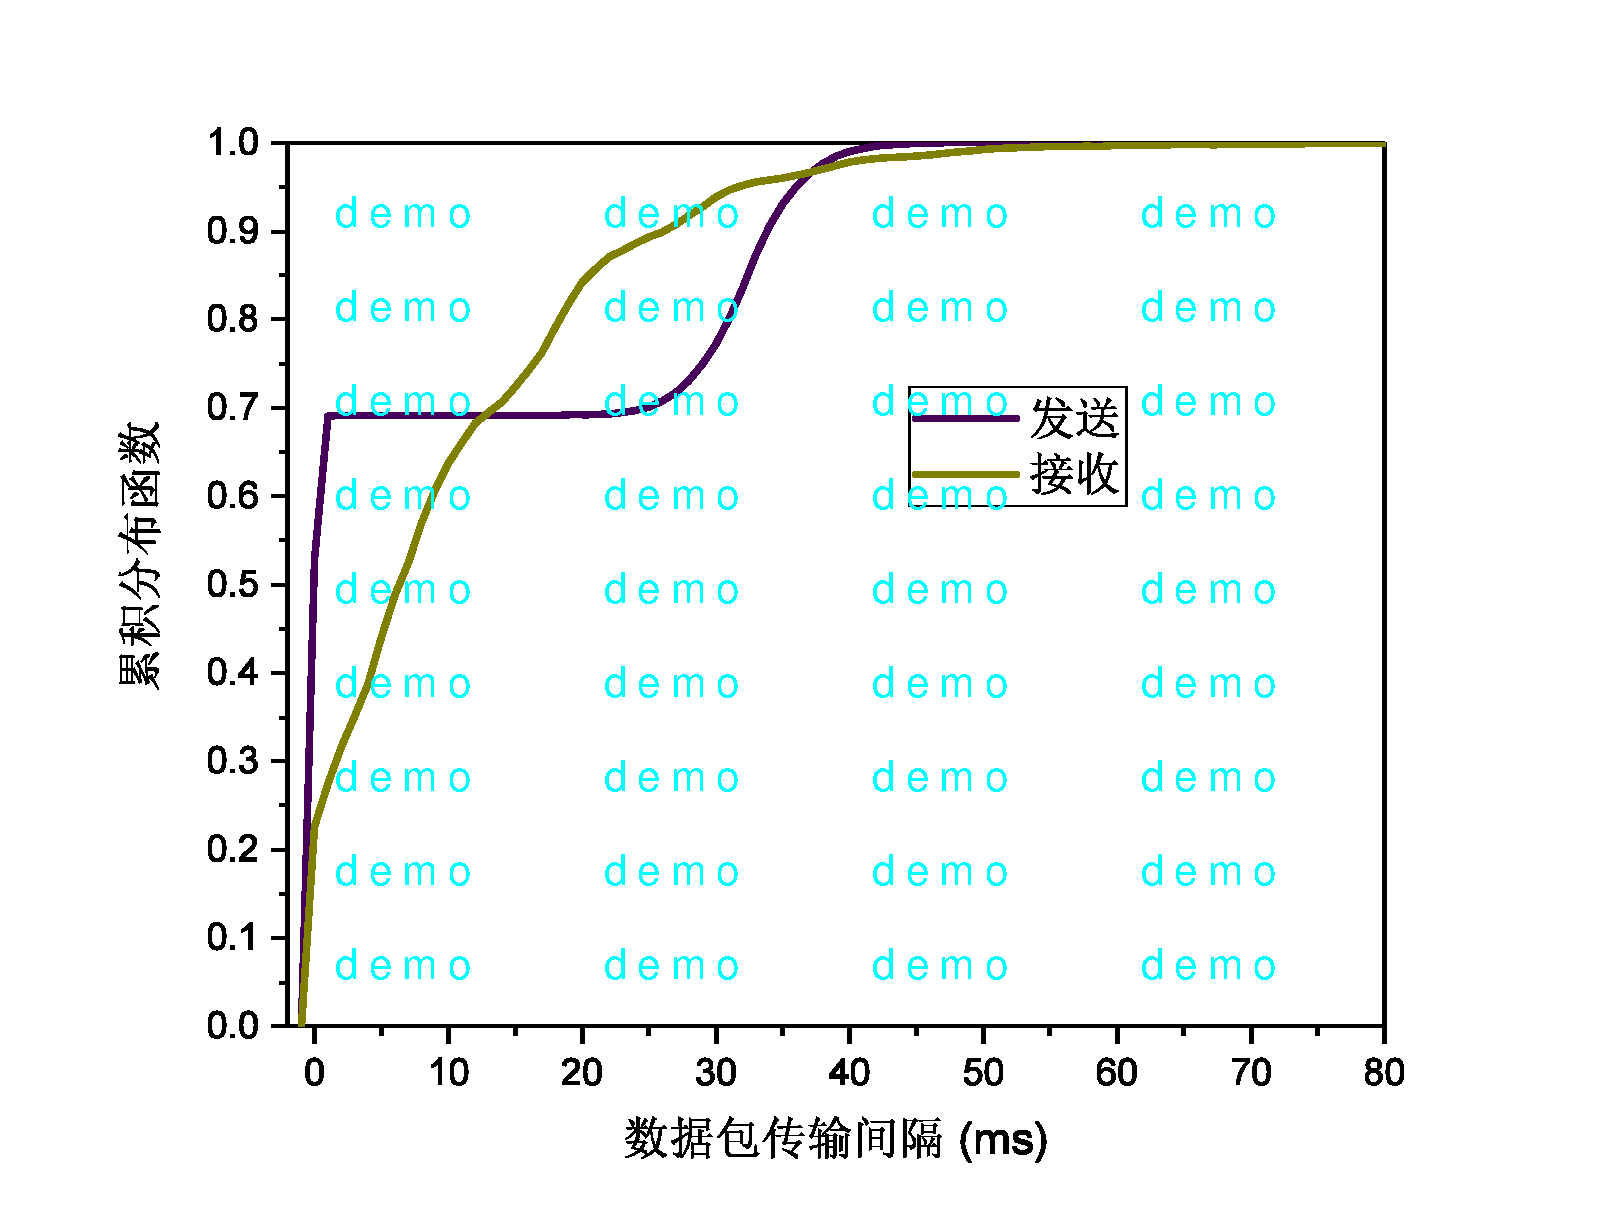
\includegraphics[width=0.7\textwidth]{chapters/chapter2/figures/cdf-send-receive.pdf}
        \caption{VoLTE视频数据包IPD的累积分布函数}\label{fig:2:cdf-ipd}
    \end{figure}
}

如图\nref{fig:2:cdf-ipd},在发送阶段,IPD主要集中在{30\ ms}及{0\ ms}两部分,由于视频刷新率为{30\ fps},每隔{33\ ms}产生一个新的视频帧,而视频帧又有多个数据包组成,造成发送阶段CDF曲线不平滑。在接收阶段,受网络噪声及传输延迟的影响,IPD在$[0,\ 30]$区间内集中分布,CDF曲线趋于平滑。因此,视频数据包在IPD方面,对时间隐通道的容忍性要优于语音数据包。

\subsubsection{VoLTE视频数据包丢包特征}
\label{chap:backinfo:volte:packets:dropout}

\insertFigure{
    \begin{figure}[htbp]
        \centering
        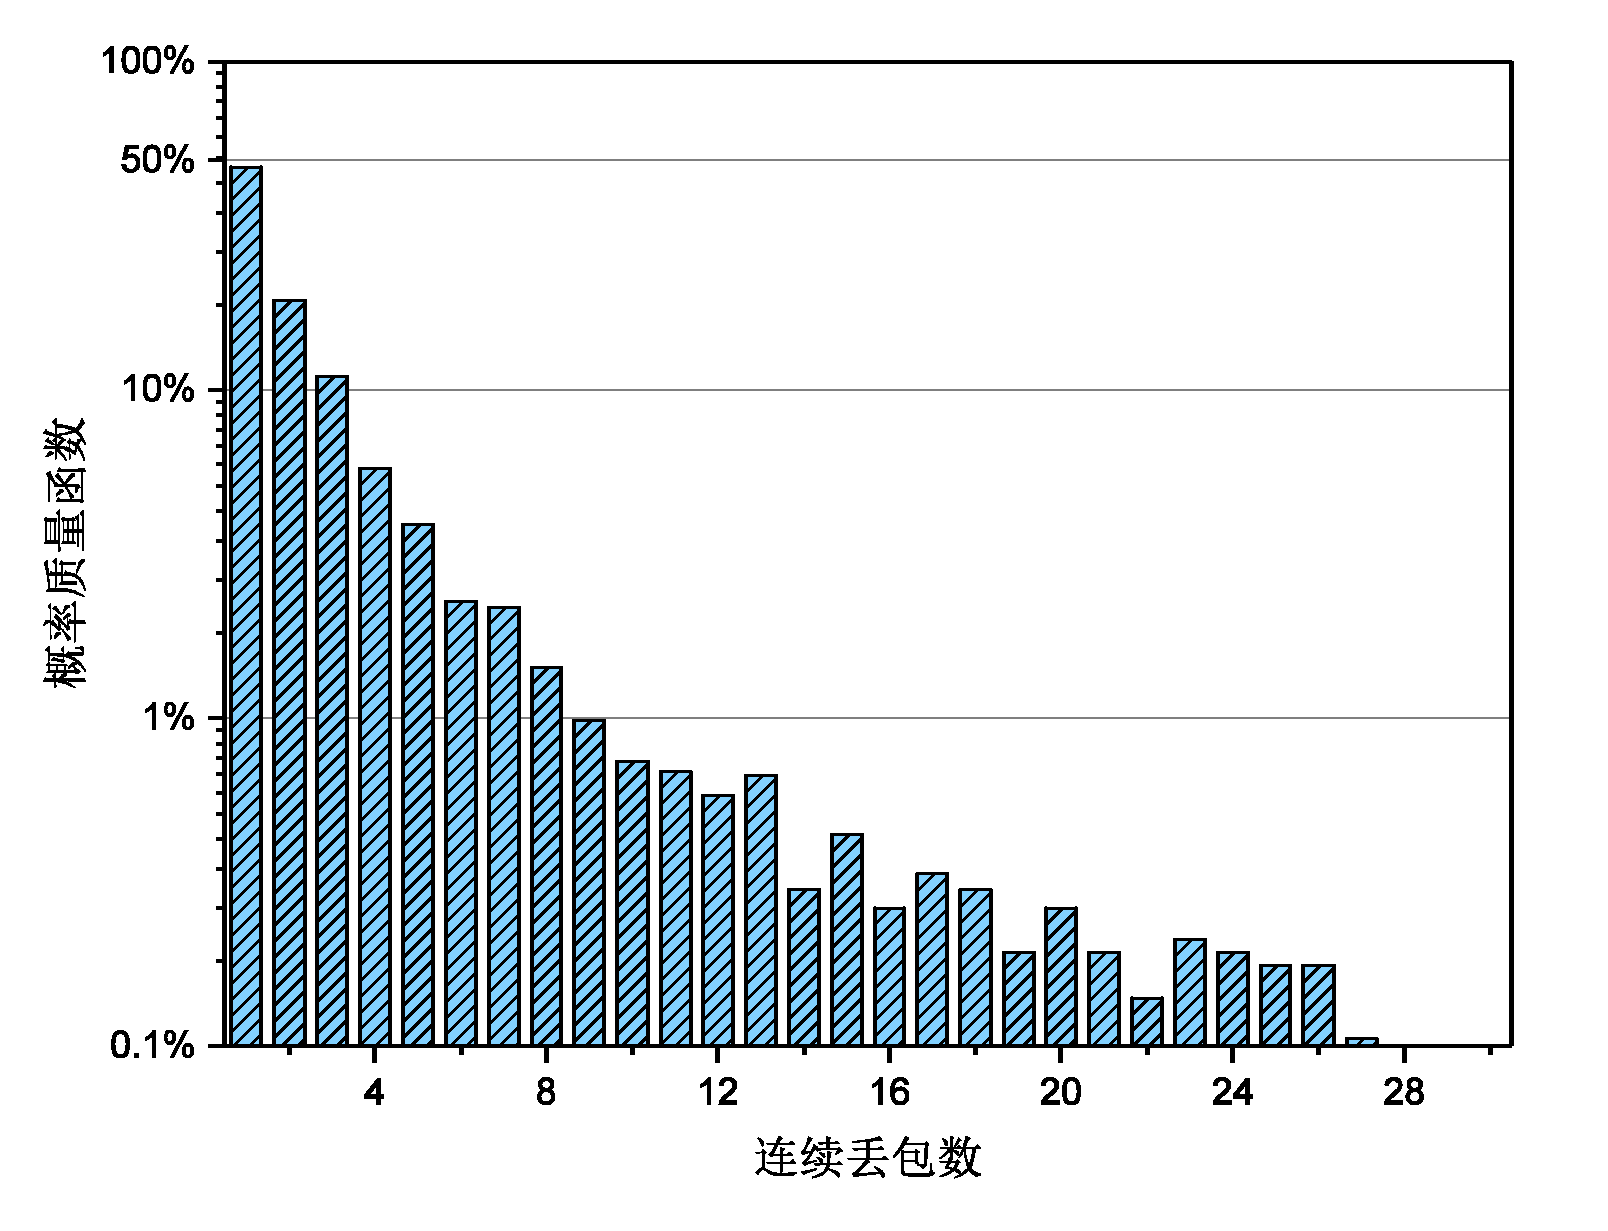
\includegraphics[width=0.7\textwidth]{chapters/chapter2/figures/pmf-dropout.pdf}
        \caption{连续丢包数量的概率质量函数}\label{fig:2:pmf-dropout}
    \end{figure}
}

对于VoLTE视频数据包,连续丢包数量的概率质量函数如图\nref{fig:2:pmf-dropout}。该统计结果,来自抓包得到的58万条VoLTE视频数据包,包含低噪声及高噪声在内的多种测试场景。PMF(Probability Mass Function)统计结果显示,VoLTE视频数据信道中的丢包事件,主要由单个离散丢包事件组成,连续大量的丢包事件占据的比例非常小。

\subsection{基于主动丢包的时间隐通道构建基础}
\label{chap:backinfo:volte:scheme}
VoLTE出现丢包的原因,主要由于通信终端与基站的空口传输过程。在复杂的无线环境中,发送端与接收端均会出现丢包可能。对于监听者,只有监听了隐通道发送方的终端设备,才有一定几率发现机遇主动丢包的时间隐通道。然而,在隐通道的威胁模型及实际应用中,监听者主要监听的是中间介质,基于主动丢包的时间隐通道,符合VoLTE的传输特征。

通过对VoLTE通话的理论及实际分析测试,在VoLTE场景中构建时间隐通道,尤其是通过主动丢包的方式构建时间隐通道,应当首先选择VoLTE视频信道作为宿主信道。与此同时,主动丢包的构建方式应当模拟离散丢包模式,并且在统计特征方面拟合已知统计结果。另一方面,VoLTE视频信道自身的丢包率,已经超过了QCI的预期丢包率,证明当前VoLTE仍然不能完全保证服务质量,通过主动丢包构建时间隐通道可行。所以,本文选择VoLTE视频信道,作为时间隐通道的宿主信道。 %VoLTE
\section{VoLTE音视频传输方案}
\label{chap:backinfo:volte}

%VoLTE实现概述

\insertFigure{
	\begin{figure}[htbp]
		\centering
        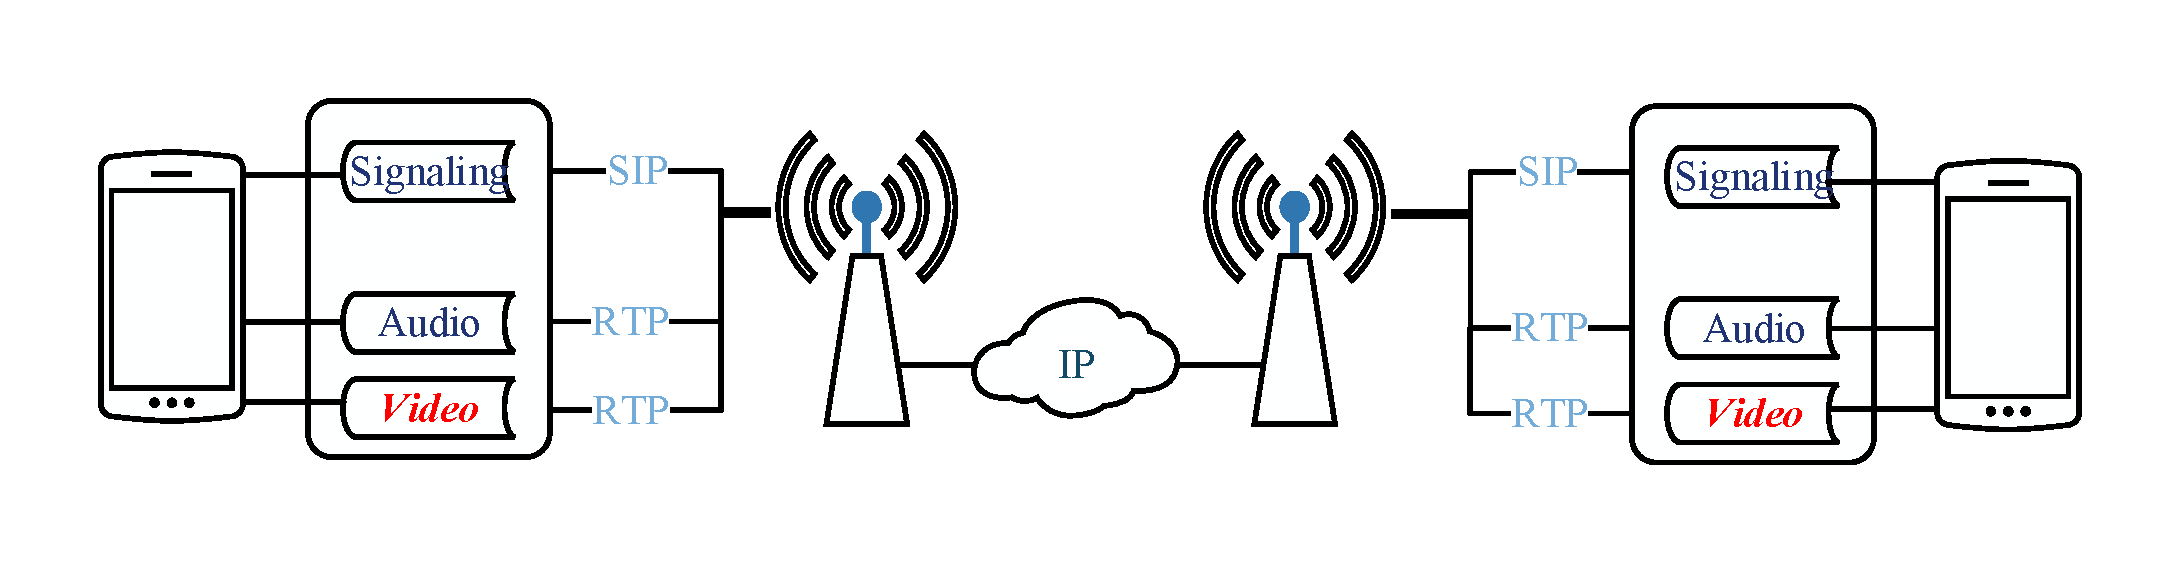
\includegraphics[width=0.95\textwidth]{chapters/chapter2/figures/volte-model.pdf}
        \caption{VoLTE视频通话中的数据流}\label{fig:2:volte-model}
	\end{figure}
}

语音通信是移动通信技术的基本需求,随着智能终端的发展,移动数据需求超过了语音通信需求。为满足用户移动宽带业务需求,基于LTE的第四代移动通信技术采用了全IP网络,实现了语音主导到数据主导的转换。新的传输模式下,LTE对数据传输进行了优化,同时提升了音视频通话业务能力。

\subsection{VoLTE数据处理流程}
\label{chap:backinfo:volte:datastream}

2G及3G时代,基于电路交换的音频通话技术,是支撑语音业务的核心解决方案。进入4G时代,核心网络已经转变为全数据包交换,基于电路交换的音频通话已经无法完全兼容,需要全新的解决方案。于是,类似VoIP音视频通话,基于LTE的VoLTE成为4G时代的音视频通话解决方案。实际应用中,支持VoLTE的终端能够快速建立呼叫,并且支持回落到3G或2G网络,从而兼容多种设备及场景\nupcite{poikselka2012voice, 8315208}。

如图\ \nref{fig:2:volte-model},VoLTE视频通话中,存在三个数据信道,分别为信令信道、语音信道及视频信道,所有的信道均通过数据包传输。采用音视频分离设计,VoLTE兼容了多种通话场景。通过信令信道协商通话模式及参数,决定语音信道及视频信道采用的编码方式。相较2G及3G网络,LTE数据上行速率得到提升,能够支撑更多的终端进行高清晰度通话\nupcite{ZHANG201929}。

\insertTable{
    \begin{table}[htbp]
        \centering
        \caption{LTE业务QCI分配表概述}
        \label{tab:2:qci-classification}
        \begin{threeparttable}
            \begin{tabular*}{\textwidth}{@{\extracolsep{\fill}}cccccc}
                \toprule
                QCI\tnote{1}分类 & 承载要求 & 优先级 & 可接受延迟 & 可接受丢包率 & 服务对象 \\
                \midrule
                1 & 保证QoS\tnote{2} & 2 & 100 ms & $10^{-2}$ & VoLTE语音 \\
                2 & 保证QoS & 4 & 150 ms & $10^{-3}$ & VoLTE视频 \\
                5 & 不保证QoS & 1 & 100 ms & $10^{-6}$ & VoLTE信令 \\
                7 & 不保证QoS & 7 & 100 ms & $10^{-6}$ & 交互式音视频应用 \\
                \bottomrule
            \end{tabular*}
            \begin{tablenotes}
                \footnotesize
                \item[1] QCI指Quality of Service Class Identifiers,QoS分类标签
                \item[2] QoS指Quality of Service,服务质量
            \end{tablenotes}
        \end{threeparttable}
    \end{table}
}

相较于固网,移动无线网络的噪声干扰不可忽视,用户通话体验与噪声强度相关。如表\ \nref{tab:2:qci-classification},根据LTE业务分类,VoLTE信令数据包具有1级最高优先级,可接受时延为{100\ ms},可接受丢包率为$10^{-6}$;VoLTE语音数据包具有2级优先级,可接受时延为{100\ ms},可接受丢包率为$10^{-2}$;VoLTE视频数据包优先级降为4级,可接受时延为{150\ ms},可接受丢包率为$10^{-3}$\nupcite{8329138}。另一方面,即使VoIP应用的数据包经LTE网络传输,其服务质量也低于VoLTE,运营商网络只保证尽力传输。VoIP应用的音视频数据对应的优先级为7,可接受时延为{100\ ms},可接受丢包率为$10^{-6}$\nupcite{7154042,6996582,Li:2015:IVS:2810103.2813618}。

因此,VoLTE较其它VoIP应用,受网络调度产生抖动的几率要小,传输更加稳定。因此时间隐通道的操作空间较小,对构建方法提出了挑战。

\subsection{VoLTE数据包传输特征}
\label{chap:backinfo:volte:packets}
%VoLTE音视频分流处理的模式(分清楚执行组件),结合传输的逻辑设计
支持VoLTE的终端设备进行视频通话,参与通话的处理器通常由两部分组成。其中一个是AP(Application Processor)也就是应用处理器,另一个是BP(Baseband Processor)也就是基带处理器。AP执行操作系统的通用数据处理,BP负责无线通信数据处理,二者相互补充,共同完成智能终端的数据处理任务。

\insertFigure{
	\begin{figure}[htb]
		\centering
        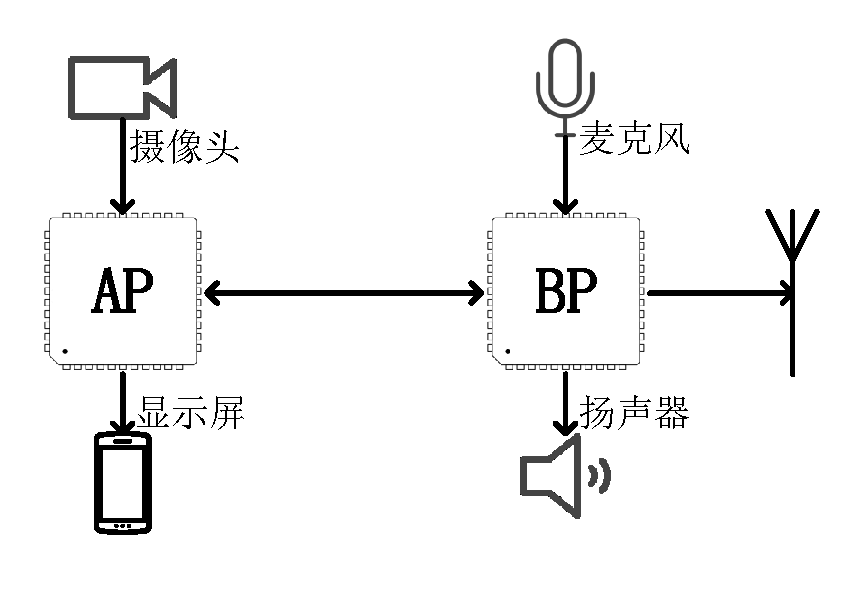
\includegraphics[width=0.55\textwidth]{chapters/chapter2/figures/ap-bp.pdf}
        \caption{VoLTE视频通话时AP与BP的功能划分}\label{fig:2:ap-bp}
	\end{figure}
}

如图\ \nref{fig:2:ap-bp},AP与BP处理不同的媒体类型。对于VoLTE语音数据,由基带处理器按照设定的时间间隔,完成模拟信号的采样、编码,并将打包好的语音数据包通过射频系统传输。对于VoLTE视频数据,由于图像处理模块集成在应用处理器中,视频数据需要应用处理器参与处理。应用处理器调用摄像系统驱动,获取编码后的视频数据,并以视频帧为单位进行打包,得到RTP视频数据包。视频数据包由系统内核中的协议栈发送,最终由BP通过射频系统传输。类似的,在接收阶段,VoLTE语音数据由基带处理器完成接收、解包、解码,并交由扬声器播放。VoLTE视频数据包则交付系统中的网络组件,完成解包、解码后,由通话软件显示在屏幕上\nupcite{ZHANG201929,guo2019volte}。

%抓包结果,分析传输特征,时间间隔、发送密度
\subsubsection{音视频数据包发送特征}
\label{chap:backinfo:volte:packets:send}

\insertFigure{
    \begin{figure}[htb]
        \centering
        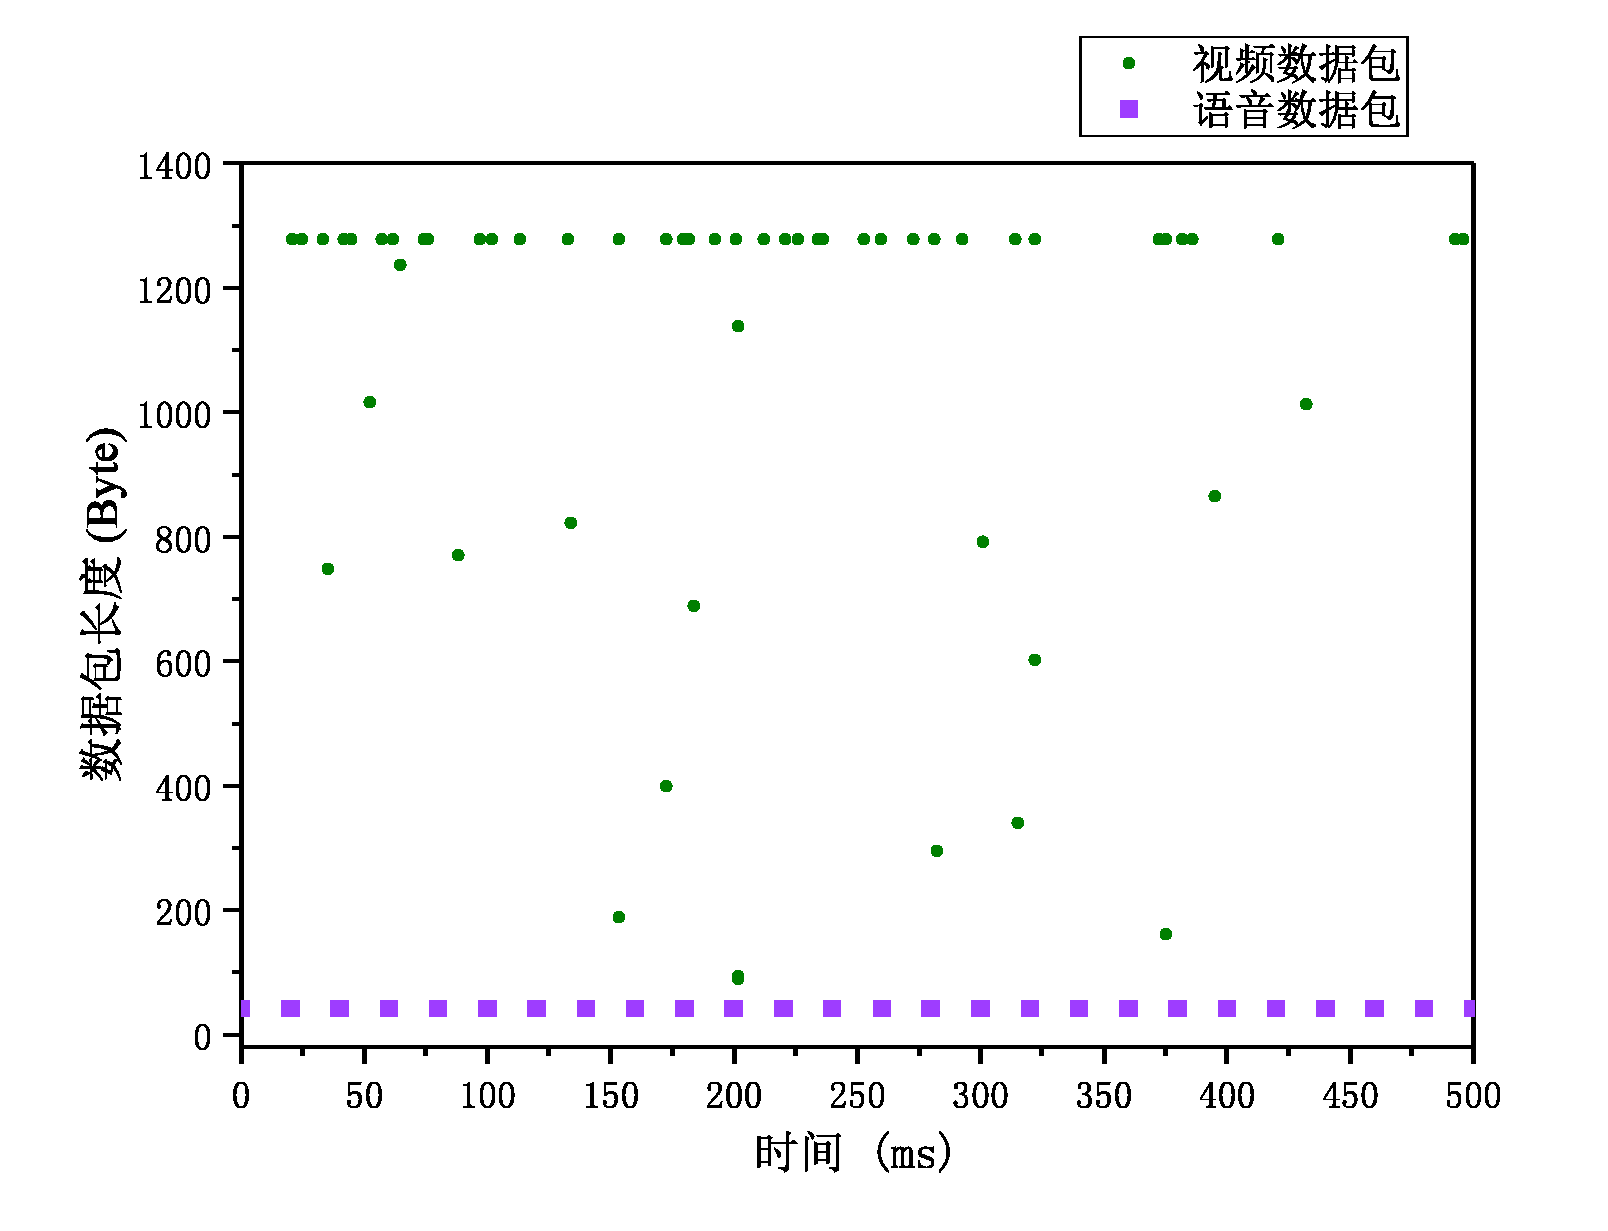
\includegraphics[width=0.75\textwidth]{chapters/chapter2/figures/length-audio-video.pdf}
        \caption{VoLTE音视频数据包发送间隔示意}\label{fig:2:audio-video}
    \end{figure}
}

对于音频数据包,采用AMR-WB格式编码时,非静音期每{20\ ms}发送一次数据包,静音期不发送数据包\nupcite{8288828}。对于视频数据包,数据包发送间隔取决于视频刷新率及编码结果,具有不确定性\nupcite{zhang2019timestamp}。如图\ \nref{fig:2:audio-video},虽然VoLTE视频数据包的长度多在{1300\ 字节}左右,但仍有部分数据包的长度随机变化;另一方面,VoLTE语音数据包的发送间隔具有规律性,而视频数据包多为密集发送。

\subsubsection{视频数据包IPD分布特征}
\label{chap:backinfo:volte:packets:ipd}
如本文\ \nref{chap:backinfo:volte:packets:send}所述,VoLTE语音数据包的IPD存在规律,因此不利于构建时间隐通道。研究VoLTE视频数据包的传输特征,对VoLTE时间隐通道构建方法具有重要意义。

\insertFigure{
    \begin{figure}[htb]
        \centering
        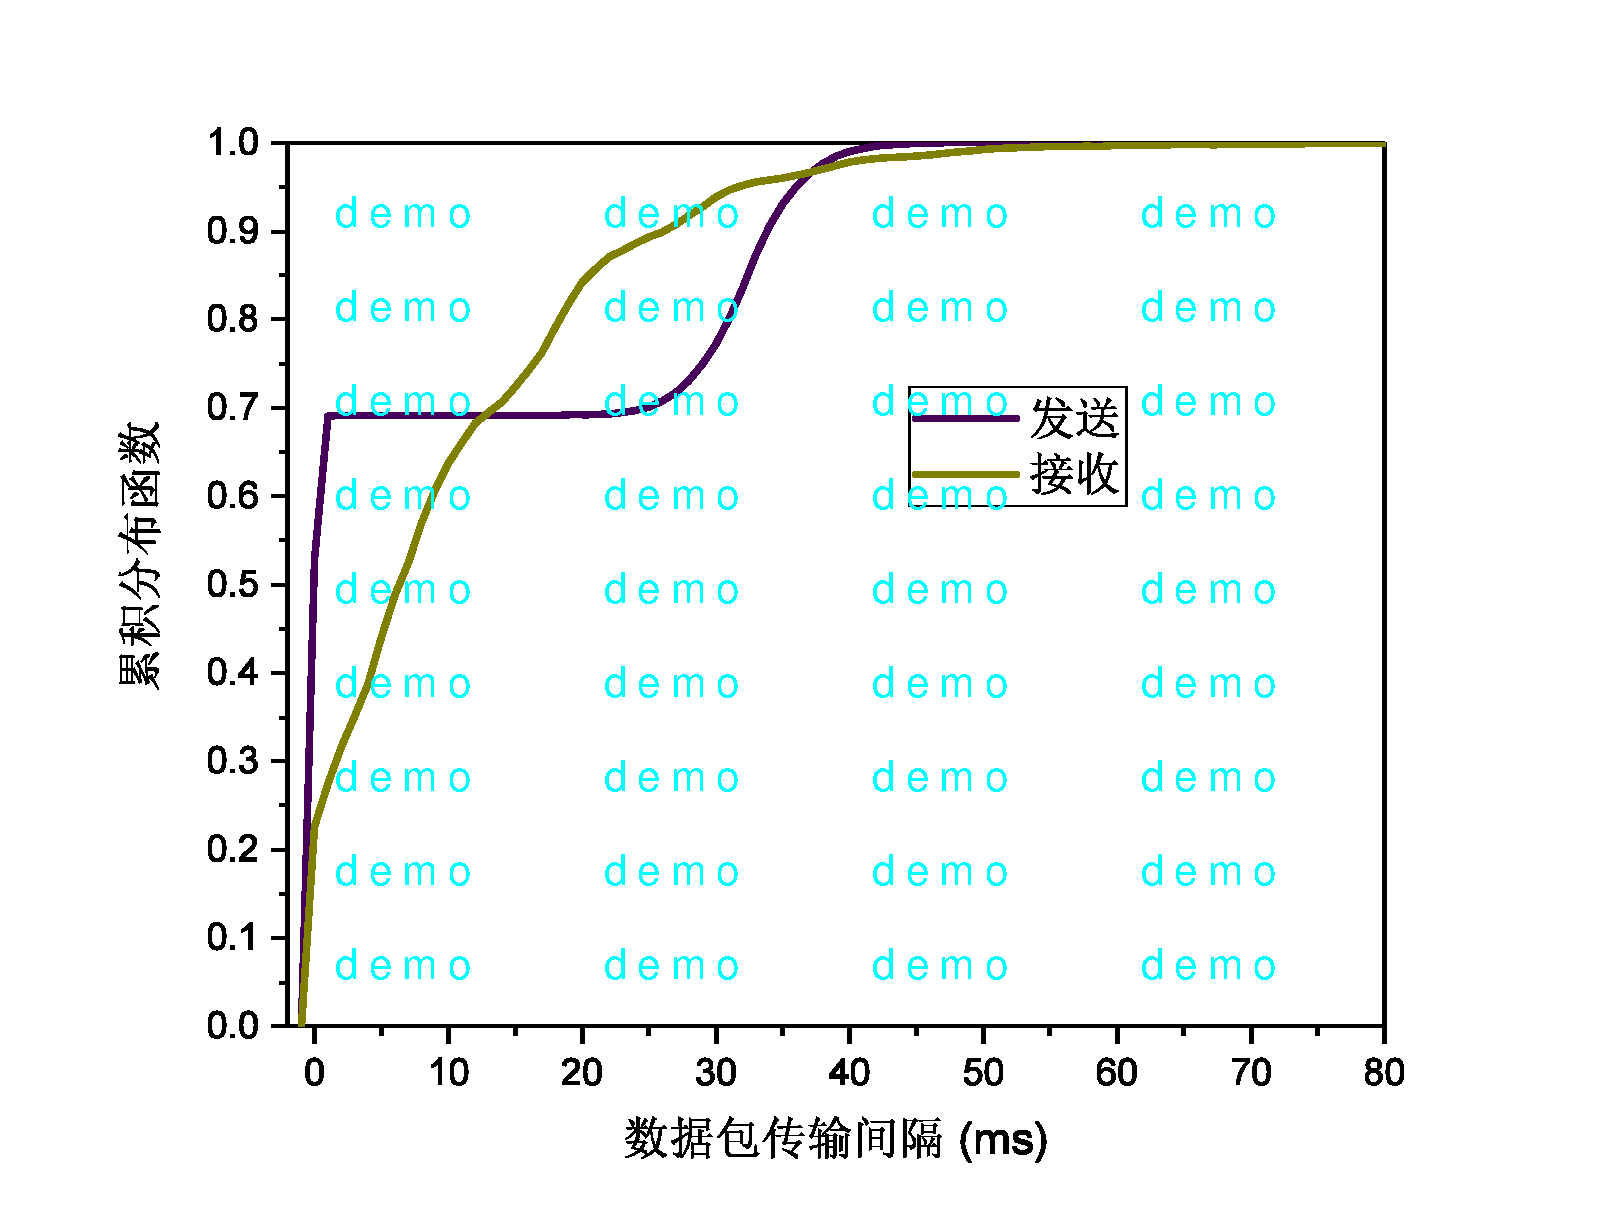
\includegraphics[width=0.7\textwidth]{chapters/chapter2/figures/cdf-send-receive.pdf}
        \caption{VoLTE视频数据包IPD的累积分布函数}\label{fig:2:cdf-ipd}
    \end{figure}
}

如图\ \nref{fig:2:cdf-ipd},发送阶段IPD主要集中在{30\ ms}及{0\ ms}。由于视频刷新率为{30\ fps},每隔{33\ ms}产生一个新的视频帧,而视频帧又由多个数据包组成,导致发送阶段CDF曲线不平滑。接收阶段,受网络噪声及传输延迟的影响,IPD集中在$[0,\ 30]$区间内,CDF曲线趋于平滑。因此在IPD方面,视频数据包对时间隐通道的容忍度高于语音数据包。

\subsubsection{VoLTE视频数据包丢包特征}
\label{chap:backinfo:volte:packets:dropout}

\insertFigure{
    \begin{figure}[htbp]
        \centering
        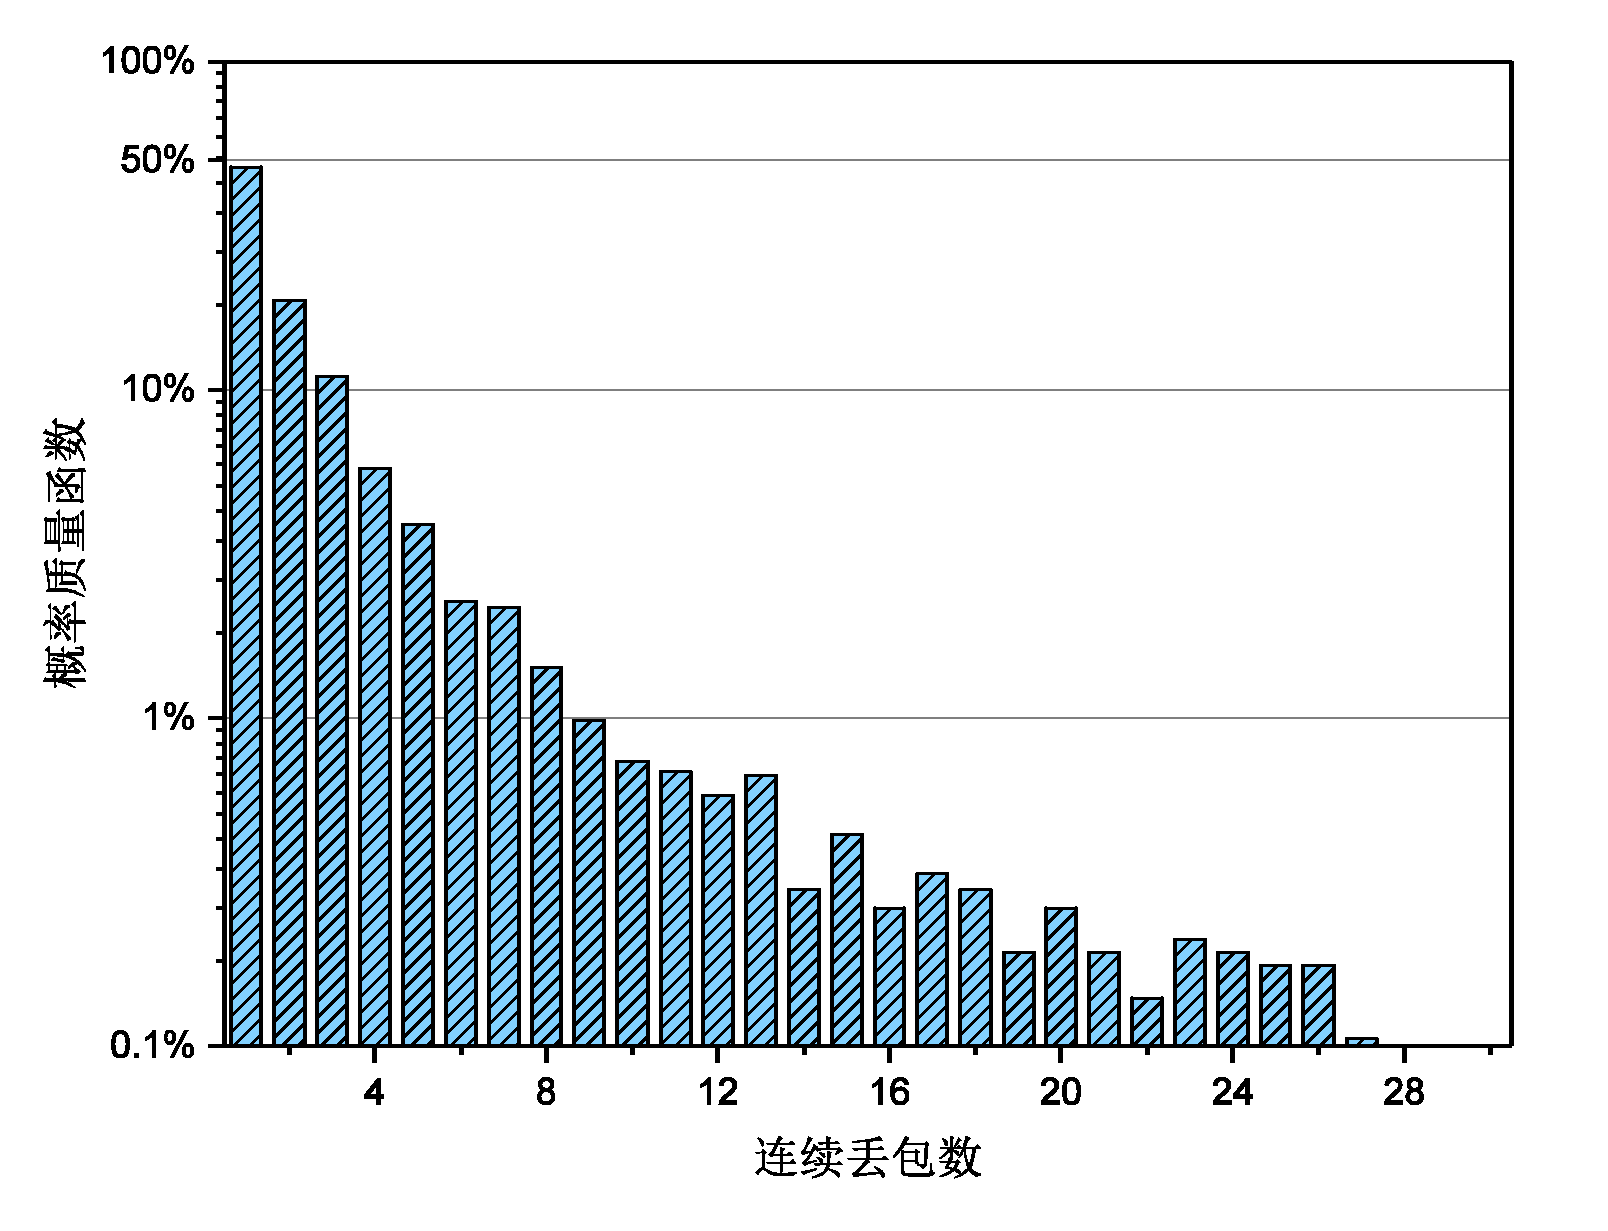
\includegraphics[width=0.7\textwidth]{chapters/chapter2/figures/pmf-dropout.pdf}
        \caption{连续丢包数的概率质量函数}\label{fig:2:pmf-dropout}
    \end{figure}
}

对于VoLTE视频数据包,连续丢包数的概率质量函数如图\ \nref{fig:2:pmf-dropout}。该统计结果,来自抓包得到的58万条VoLTE视频数据包,包含低噪声及高噪声在内的多种测试场景。PMF(Probability Mass Function)统计结果显示,VoLTE视频信道中的丢包事件,主要由单个离散丢包事件组成,连续丢包事件占据的比例较小。

\subsection{基于主动丢包的时间隐通道构建}
\label{chap:backinfo:volte:scheme}
VoLTE出现丢包的原因,主要是终端与基站空口传输过程的干扰。复杂的无线网络环境中,发送端与接收端均存在丢包可能性。对于监听者,只有监听了隐通道发送方的终端设备,才有一定几率发现基于主动丢包的时间隐通道。然而,在隐通道威胁模型及实际应用中,监听者主要监听中间媒介,因此基于主动丢包的时间隐通道,只需要保证统计特征方面的一致性即可。

通过对VoLTE通话的理论及数据分析,在VoLTE场景中构建时间隐通道,尤其是通过主动丢包的方式构建时间隐通道,应当选择VoLTE视频信道作为宿主信道。与此同时,主动丢包的结果应当模拟离散丢包模式,并且在统计特征方面拟合已知结果。另一方面,VoLTE视频信道的丢包率,已经超过了QCI的预期丢包率,表明当前LTE网络不能完全保证服务质量,通过主动丢包构建时间隐通道可行。 %CTC
\section{VoLTE传输协议分析}
\label{chap:backinfo:rtp}

VoLTE实在RTP协议的基础上实现的,RTP自身有一些特征

在这里进行的分析,如何利用这些特征,构造时间隐通道

\subsection{RTP数据包结构}
\label{chap:backinfo:rtp:struct}

RTP是怎样的标准,数据包等层次解析

RTP头的组成

\subsection{随机字段}
\label{chap:backinfo:random}

RTP参数中,包含哪些随机生成的字段

SSRC、TimeStamp,生成的效果

可以用于时间隐通道的秘钥及随机特征生成,保证保密性

\subsection{RTP丢包处理}
\label{chap:backinfo:dropout}

RTP及应用中,对于丢包事件的处理

丢包不重传,序号保证自增,是主动丢包方法的基础
 %RTP
\section{时间隐通道检测方法}
\label{chap:backinfo:detect}

%本节主要介绍,现有的时间隐通道检测方法,主要包括哪些
时间隐通道的发展,催生了新的时间隐通道检测技术。基于统计及分布一致性的时间隐通道检测方法,是常用的检测方法。某些场景中,基于标准差的检测方法,以及基于机器学习的检测方法也是有效的。\nupcite{ARCHIBALD2014284}

\subsection{基于分布曲线的检测}
\label{chap:backinfo:detect:statistical}

%统计看CDF差异,主要评估了哪些参数
传输过程中的时间特征,是时间隐通道检测方法的检测目标,基本的检测对象为IPD。当传输延迟恒定时,发送方观测到的IPD分布与接收方观测到的IPD分布是一致的。然而,存在网络噪声或者时间隐通道时,IPD分布出现偏离。时间隐通道检测方法,通过对比分布之间的最大偏离程度,从而判断是否存在隐通道。
\insertEquation{
    \begin{equation}
    \label{equ:2:ks}
		D_{KS}\ =\ sup_{x}\ |F_{1,\ n}(x)\ -\ G_{1,\ m}(x)|
    \end{equation}
    \begin{equation}
    \label{equ:2:ks-p}
        D_{KS,\ 0.05}\ =\ 1.358\ \times\ \sqrt{\frac{n\ +\ m}{n\ \times\ m}}
    \end{equation}
}
\insertFigure{
	\begin{figure}[htbp]
		\centering
        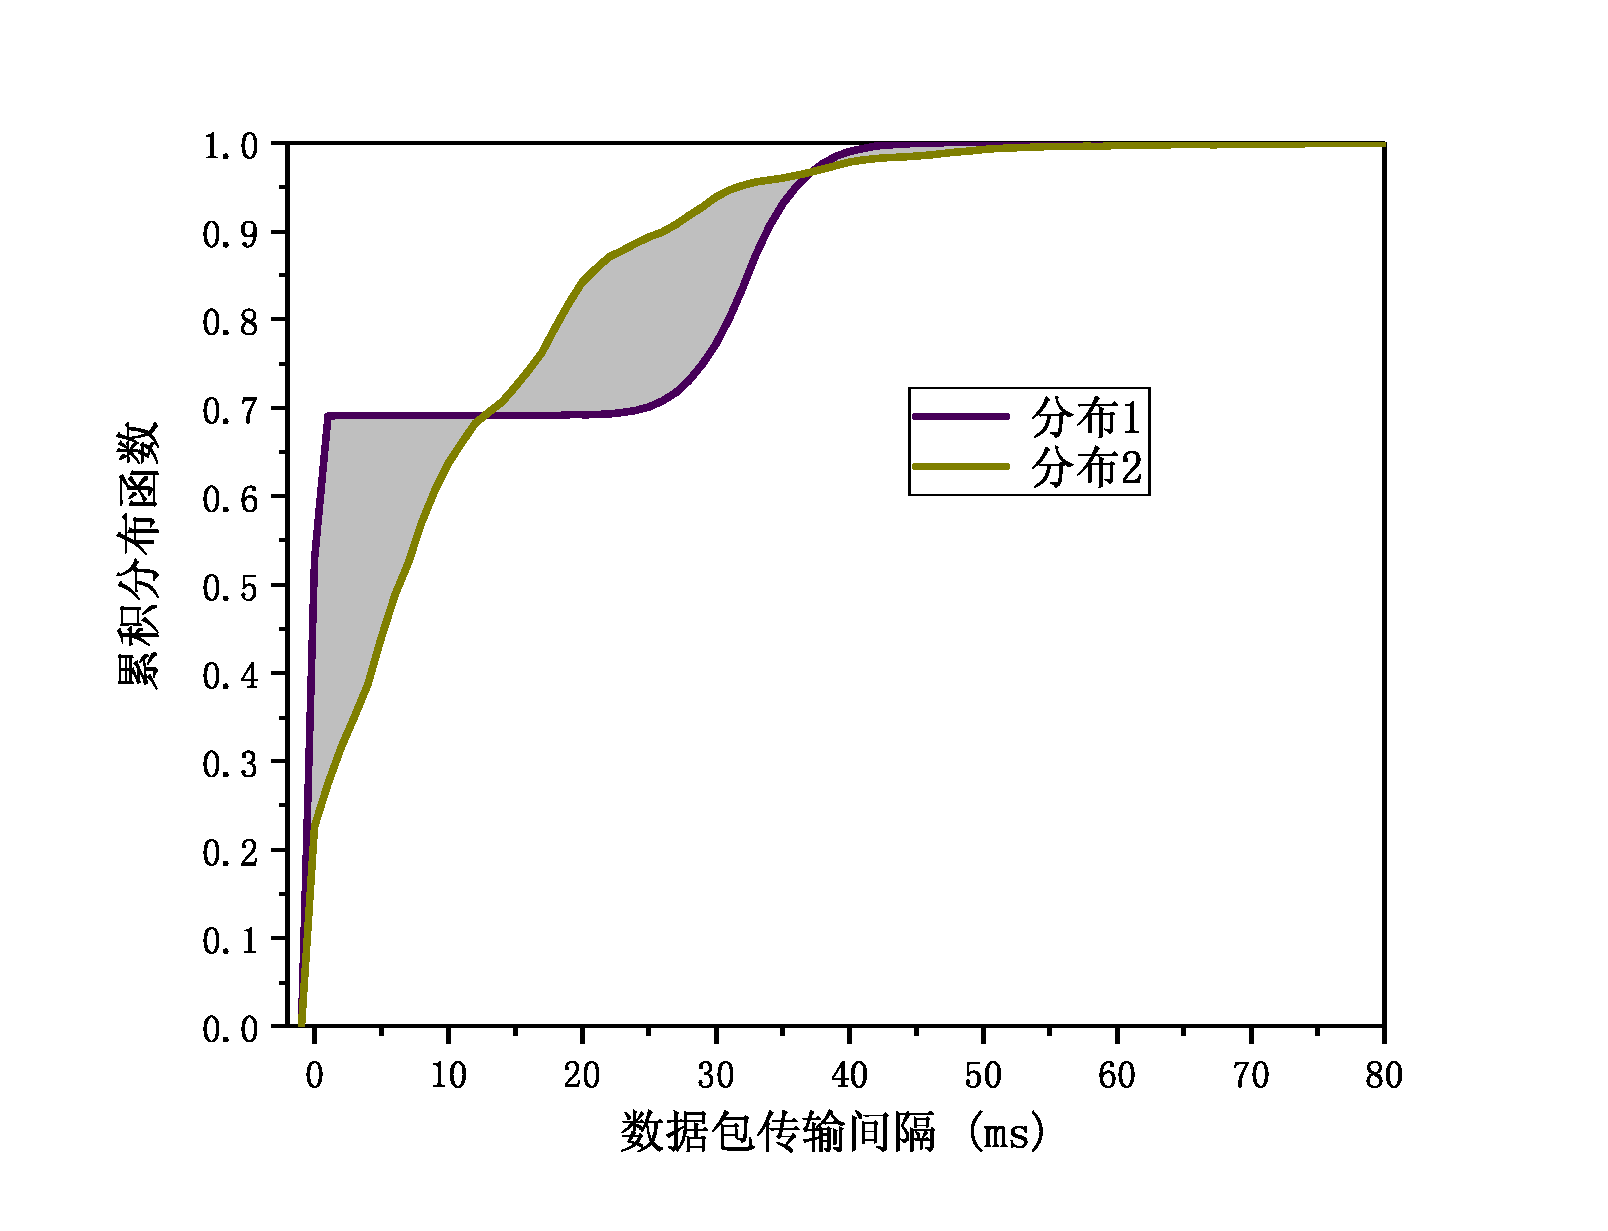
\includegraphics[width=0.7\textwidth]{chapters/chapter2/figures/ks-cdf.pdf}
        \caption{CDF曲线差异示意图}\label{fig:2:ks-cdf}
	\end{figure}
}

%如何根据差异,判断一致性
如图\nref{fig:2:ks-cdf},不同的CDF曲线代表不同的IPD分布。通过公式(\nref{equ:2:ks}),计算CDF曲线差异绝对值的最大值,得到分布曲线之间的直接差异。根据一致性假设理论,进行K-S检验的两个样本,在{95\ \%}几率一致的假设前提下,通过公式(\nref{equ:2:ks-p})计算置信值$D_{KS,\ 0.05}$。当$D_{KS,\ 0.05}\ >\ D_{KS}$时,即可判定$F_{1,\ n}$与$G_{1,\ m}$属于相同分布。

除了K-S检验外,常用的双样本检验方法还包括{Welch's\ \ t检验}、Epps-Singleton检验、Mann-Whitney rank检验及Wilcoxon rank检验等。不同检验方法与适用的分布类型对应,应用中要考虑检测对象的分布情况。当检测样本与参照样本通过了检验,则证明二者在分布方面没有差异,存在隐通道的概率较小。

\subsection{基于熵的检测}
\label{chap:backinfo:detect:entropy}

%计算熵,判断的对象是什么
统计学中,Kullback–Leibler散度又称相对熵,是一种判断概率质量函数差异的方法。实际应用中,通过计算样本之间相对熵值大小,判断分布之间的一致性。\nupcite{5590253,Gianvecchio:2007:DCT:1315245.1315284,Cabuk:2004:ICT:1030083.1030108,6296078}
\insertEquation{
    \begin{equation}
    \label{equ:2:kld}
		D_{KL}(F(x)\ ||\ G(x))\ =\ \sum_{x=i}\ f(x)\ \times\ \log \frac{f(x)}{g(x)}
	\end{equation}
}
\insertTable{
	\begin{table}[htbp]
        \centering
        \caption{IPD的概率质量函数示意表}
        \label{tab:2:pmf-dis}
        \begin{tabular*}{0.6\textwidth}{@{\extracolsep{\fill}}ccc}
        \toprule
        IPD & f(x) & g(x)\\ 
        \midrule
        0 & 0.52921 & 0.2265 \\ 
        1 & 0.16155 & 0.04827 \\ 
        2 & 0.00075 & 0.04231 \\ 
        3 & 0.00011 & 0.03467 \\ 
        4 & 0.00002 & 0.03603 \\ 
        5 & 0.00002 & 0.05287 \\ 
        \bottomrule
        \end{tabular*}
    \end{table}
}

如表\nref{tab:2:pmf-dis}所示,概率质量函数PMF(Probability Mass Function)对应的是不同IPD的概率,参照分布的概率函数为$g(x)$,样本分布的概率函数为$f(x)$。通过公式(\nref{equ:2:kld})计算$D_{KL}$,得到结果$0.278$,高于检测阈值$0.1$\nupcite{ZHANG201866},因此得出结论,样本与参照分布不一致,存在隐通道的概率较高。

\insertTable{
	\begin{table}[htbp]
        \centering
        \caption{经典时间隐通道的检测准确率}
        \label{tab:2:test-results}
        \begin{tabular*}{0.6\textwidth}{@{\extracolsep{\fill}}cccc}
            \toprule
            检验方法 & JitterBug\nupcite{shah2006keyboards} & TR-CTC\nupcite{Cabuk:2004:ICT:1030083.1030108} & MB-CTC\nupcite{10.1007/978-3-642-16435-4_15} \\ 
            \midrule
            K-S检验 & 0.66 & - & 0.56 \\
            T检验 & 0.86 & 0.56 & 0.95 \\
            K-L散度 & 0.62 & 0.56 & 0.65 \\
            \bottomrule
        \end{tabular*}
    \end{table}
}

如表\nref{tab:2:test-results},对于SSH场景中的几种经典时间隐通道,不同检验方法的准确率存在差异。\nupcite{ARCHIBALD2014284}由于TR-CTC不改变分布特征,因此通过K-S检验及T检验检测准确率较低。K-L散度对概率变化更敏感,计算过程不仅考虑了概率本身,概率所占的比重也同时纳入计算,因此具有较均衡的检测能力。对比结果可见,结合不同的检测方法的优势,能够在检测原理上互补,具有更好的检测效果。

\subsection{基于机器学习的检测}
\label{chap:backinfo:detect:machine}

%机器学习的模型是怎样生成的
基于机器学习的时间隐通道检测方法,需要预先获取宿主信道的传输特征,然后训练对应的模型。对于监听者,基于统计的时间隐通道检测方法针对的是特定隐通道,并且在获取足够统计数据后才具有较好的效果。而基于机器学习的时间隐通道检测方法,在完成模型训练后,具备实时检测能力,并且不受隐通道类型的限制。\nupcite{8875875,7087364}

%判定结果如何认定是否通过
基于SVM(Support Vector Machines)的检测方法,通过提取样本中的特征向量,根据训练的SVM分类器进行检测。检测过程中,提取样本的指纹特征,通过训练过的SVM进行分类判断。在已知时间隐通道的基础上,生成各种隐通道的传输特征,计算其K-S结果、K-L散度及统计规律等特征,得到数据集并训练SVM分类器。\nupcite{7087364}基于SVM检测方法,在盲测情况下具有较好的效果,对于传输特征稳定的信道来说,具备良好的检测结果。

VoLTE视频通话中,语音信道具有明确的规律性,现有的检测方法均可进行判别。然而视频信道中,无法提取出明确的传输特征。因此,VoLTE视频信道中的时间隐通道检测,无法以局部特征代替全局特征,需要在一定规模统计数据的基础上进行分布检验。 %Detect
\section{时间隐通道评价指标}
\label{chap:backinfo:metric}

%构建一个好的时间隐通道,应当满足的指标是什么
时间隐通道作为一种隐蔽传输方法,对其基本要求是隐蔽性,也就是抗检测能力。与此同时,传输可靠性,也就是鲁棒性,在高噪声环境中也非常重要。为满足数据传输的需要,传输性能应当达到一定的传输速率。此外,时间隐通道构建过程产生的代价,以及数据保密性也是重要的评估指标。

\subsection{抗检测能力}
\label{chap:backinfo:metric:undetectability}

%抗检测能力方面,如何通过现有检测方法
时间隐通道的抗检测能力指标,要求隐通道的传输特征与宿主特征保持一致。通用的特征包括IPD及数据包发送顺序,在VoLTE音视频通话中,重点关注接收过程的IPD分布。对于基于主动丢包的时间隐通道,由于增加了丢包数量,因此丢包分布也是检测特征之一。

%如何在特征分布上,与已知统计结果保持一致
合理的抗检测能力评估,首先应该分析宿主信道的传输特征,并将其作为标准参照。在VoLTE场景下,需要持续观测才能得到样本分布。分布对比过程中,通过本文\nref{chap:backinfo:detect}中列举的方法,由多重维度进行综合评估。对于时间隐通道构建方法,应当具备可调的传输参数,从而应对不同的网络场景,提高自身隐蔽性。

\subsection{鲁棒性}
\label{chap:backinfo:metric:robustness}

%网络噪声不可避免,连续丢包数也是不断变化的
网络噪声是不可避免的,信道中的主动监听者也会采取措施破坏隐通道。时间隐通道的抗噪声干扰能力,对隐通道的应用范围及可靠性有重要意义。
\insertEquation{
    \begin{equation}
    \label{equ:2:ber}
		BER\ =\ \frac{error\ bits}{sent\ bits}\quad (\%)
	\end{equation}
}
%如何完成有效传输的同时,减低误码率,并具备抵御强网络噪声的能力
鲁棒性测试,通常在不同噪声强度下进行,通过隐通道的调制与解调测试,计算传输错误的比例。公式(\nref{equ:2:ber}),是通用的BER(Bit Error Rate)计算公式,反映了时间隐通道的抗噪声干扰能力。

\subsection{传输性能}
\label{chap:backinfo:metric:throughput}

%时间隐通道自身的性能,相较存储隐通道较低
相较于存储隐通道,时间隐通道在性能方面存在劣势。\nupcite{mazurczyk2016youskyde,7122356}时间隐通道受限于承载对象的传输速率,存在性能上限。与此同时,时间隐通道的抗检测能力、鲁棒性和传输性能难以兼顾,牺牲性能保证可用性是常用的解决方式。
\insertEquation{
    \begin{equation}
    \label{equ:2:bps}
        Throughput\ =\ \frac{sent\ bits}{time}\quad (bps)
    \end{equation}
    \begin{equation}
    \label{equ:2:bpp}
        Capacity\ =\ \frac{sent\ bits}{sent\ packets}\quad (bpp)
    \end{equation}
}
%应当达到怎样的指标,从而满足实际应用要求
传输性能的评估指标,通常包括传输速率及信道容量。传输速率代表每秒传输的数据位数,以bps(bits per second)为单位,计算方法如公式(\nref{equ:2:bps})。有效的时间隐通道,传输速率应达到{1\ bps}左右。\nupcite{6296078,LIANG2018162,ZHANG201866}时间隐通道中,信道容量代表每个数据包的嵌入位数,通常以bpp(bits per packet)为单位,计算方法如公式(\nref{equ:2:bpp})。

\subsection{构建代价}
\label{chap:backinfo:metric:cost}

%构建时间隐通道以后,对传输效果的影响
对于实时应用,用户对传输质量较为敏感。时间隐通道产生的构建代价,不应超过网络噪声产生的损失。对于VoLTE通话,用户对音视频质量的评价能够有效反映构建代价。\nupcite{8288828}

%是否造成传输质量大幅度降低
通过主动丢包的方式构建时间隐通道,产生的直接影响是丢包率升高,侧面影响是音视频质量的降低。稳定的网络环境中,应当减少主动丢包的比例,反之亦然。丢包必然导致数据损失,语音通话中表现为语音缺失,视频通话中表现为画面卡顿或残影。当前关于图像及视频质量的客观评价方法,能够在一定程度上反映通话质量,从而判断构建过程产生的代价。

\subsection{保密性}
\label{chap:backinfo:metric:non-disclosure}

%保密性要求,中间人截获,并且知晓方案,如何保证信息不泄露
隐通道的存在,迫使监听者对信道安全进行分析,甚至采取主动防御的方式进行削弱。根据监听者参与程度的差异,可以划分为主动式监听者及被动式监听者。被动式监听者主要对传输特征进行分析,进行数据审计。主动式监听者采取防范手段,对可能的隐通道进行阻止,通常采用数据覆写及数据包缓冲等操作。\nupcite{MAZURCZYK2019712,8786254}

%面对防御措施,不能破坏,主动监听者及被动监听者
更重要的是,当监听者已经发现了隐通道的存在,并且通过某种途径获知了隐通道的构建原理,仍要保证隐蔽消息的安全性。除了基本的加密措施,隐通道的各阶段应具备随机性,引入CSPRNG(Cryptographically Secure Pseudo-Random Number Generator)随机数发生器,打乱数据之间的线性关联。 %Metric
\chapter{VoLTE主动丢包时间隐通道的检测方法}
\label{chap:analyze}

本章主要介绍主动丢包时间隐通道的检测方法,适用于VoLTE视频信道。

%在下方加入各小节内容
\section{概述}
\label{chap:analyze:overview}

%为什么要对丢包的特征进行检测
研究面向基于主动丢包的VoLTE时间隐通道的检测方法,对改进时间隐通道构建方法,提高抗检测能力有正向促进意义。在VoLTE视频信道中,尤其对于采用了主动丢包的时间隐通道,时间隐通道对IPD分布产生的影响有限。因此,基于IPD的时间隐通道检测方法,忽略了丢包特征,检测效果较差。针对该类时间隐通道,需要设计一种综合的检测方法,结合不同的检测工具对多种分布特征进行检测。

\insertFigure{
	\begin{figure}
		\centering
        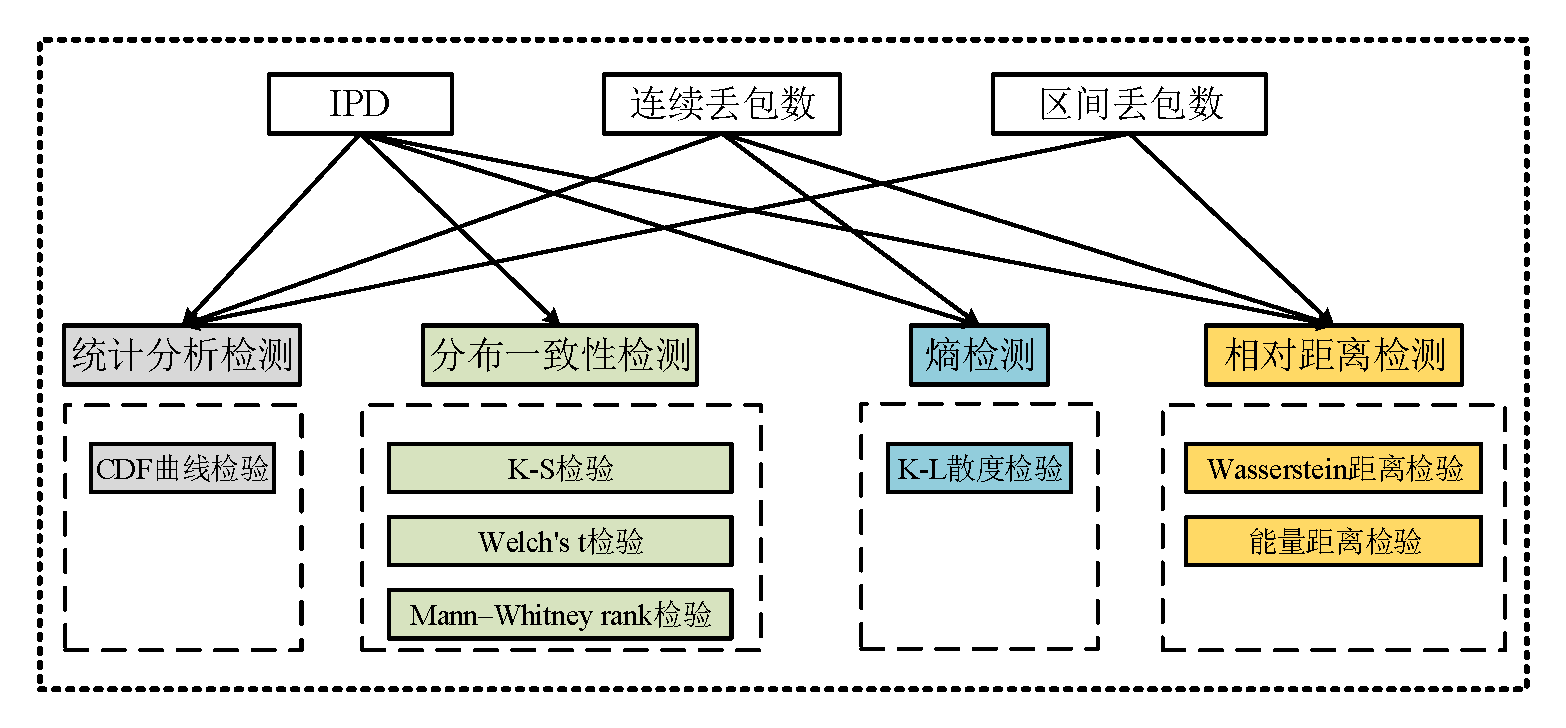
\includegraphics[width=0.9\textwidth]{chapters/chapter3/figures/struct.pdf}
        \caption{面向基于主动丢包的VoLTE时间隐通道检测方法结构图}\label{fig:3:struct}
	\end{figure}
}

%检测主要从IPD、丢包特征及突发丢包几个方面展开
丢包事件发生后,产生的影响体现在IPD分布、突发丢包长度,以及区间丢包数分布。如图\nref{fig:3:struct},本检测方法的检测对象包括IPD、突发丢包长度及区间丢包数三种。采用的检测方法分为四类,分别为统计分析检测、分布一致性检测、熵检测及相对距离检测。基于IPD的检测,是时间隐通道的基本检测方法。基于突发丢包长度的检测,重点在于判断不同突发长度的概率,因此适用统计分析检测、熵检测及相对距离检测。基于区间丢包数的检测,重点在于判断分布之间的差异,因此适用统计分析检测及相对距离检测。
%通过模拟测试,该评估方法具备可行性
为测试该方法的可用性,模拟主动丢包的时间隐通道进行了测试。通过一系列模拟实验,证明该方法在综合了各维度特征后,提升了检测能力,对基于主动丢包的时间隐通道具有良好的分辨能力。
\section{研究背景和动机}
\label{chap:analyze:motivation}

%当前通过主动丢包方式,构建时间隐通道的方法比较少,缺少对应的检测方法
时间隐通道检测方法,与时间隐通道构建方法是对应的。传统时间隐通道的调制对象为IPD,有多种检测方法与之对应\nupcite{Cabuk:2004:ICT:1030083.1030108,6222709,Gianvecchio:2007:DCT:1315245.1315284,ARCHIBALD2014284,7346833}。这些方法的模式是相似的,首先统计宿主信道的IPD分布特征,生成标准参照。对于检测样本,统计其IPD分布得到CDF曲线或PMF曲线,通过对比标准参照判断是否存在时间隐通道。

VoLTE视频通话中,丢包事件对IPD分布的影响有限。但发生丢包事件时,产生了可观测的连续丢包数及区间丢包数。网络噪声越强,丢包数越多,观测到的分布差异越大。另一方面,由于网络抖动导致的丢包,通常集中在一定区间内。将数据包划分为独立区间,分别统计区间内的丢包数量,并将所有区间的统计结果汇总,得到区间丢包数的统计分布。由于基于主动丢包的时间隐通道通常存在固定的丢包周期,因此区间丢包数普遍增加,较参照分布存在差异。

%研究的重点,是在VoLTE场景下,构建一套时间隐通道的检测方法
除了观测对象的差异,传统检测方法采用的数学方法比较单一,检测效果不够全面\nupcite{5590253,Gianvecchio:2007:DCT:1315245.1315284,7427126,7827996}。除了常用的分布曲线检测、基于熵的检测,相对距离检测也是有效的判别方法\nupcite{ramdas2015wasserstein,10.5555/2926296.2926299,bellemare2017cramer}。

%并作为基础,验证后续的时间隐通道构建方法
该检测方法中,评估了多种观测对象,并且结合了多维度的评估方式,提升了对主动丢包时间隐通道的检测能力。模拟实验证明,该方法的检测子项能够相互补充,有效提高了检测精度。此外,该方法用于验证本文提出的构建方法,评估抗检测能力方面是否符合指标要求。
\section{VoLTE丢包的统计分析}
\label{chap:analyze:results}

%通过抓包测试,得到了一些VoLTE视频流结果
在研究检测方法前,首先分析统计特征并构造参照数据集。以三星A5108手机为平台,进行不同网络场景下的视频通话,并通过tcpdump抓包软件\nupcite{10.5555/1047846.1047873}捕获所有的视频数据包,得到实验数据集。

%分析抓包结果,对特征进行分析
\insertTable{
	\begin{table}[htbp]
        \centering
        \caption{VoLTE视频通话抓包结果}
        \label{tab:3:capture-results}
        \begin{threeparttable}
            \begin{tabular*}{0.8\textwidth}{@{\extracolsep{\fill}}ccccc}
            \toprule
            场景 & 通话次数 & 数据包总数 & 抓包总数 & 平均丢包率 \\ 
            \midrule
            Excellent & 13 & 323297 & 320990 & 0.71\ \% \\ 
            Good & 17 & 288592 & 261470 & 9.40\ \% \\
            \bottomrule
            \end{tabular*}
            \begin{tablenotes}
                \footnotesize
                \item[] 视频数据包发送速率,约为100\ pkts/s
            \end{tablenotes}
        \end{threeparttable}
    \end{table}
}
如表\ \nref{tab:3:capture-results},抓包结果来自两种场景。Excellent场景对应同基站通话,网络环境稳定;Good场景对应跨基站通话,网络噪声较强。Excellent场景中,通话质量及流畅度较好,并且丢包率较低;Good场景中,偶尔存在卡顿或图像模糊,丢包率较高。两种场景中的统计特征不完全相同,因此统计与检测过程分开进行。

\subsection{丢包率}
\label{chap:analyze:results:plr}

%统计的各个通话的全局丢包率,分布情况
\insertFigure{
	\begin{figure}[htbp]
		\centering
        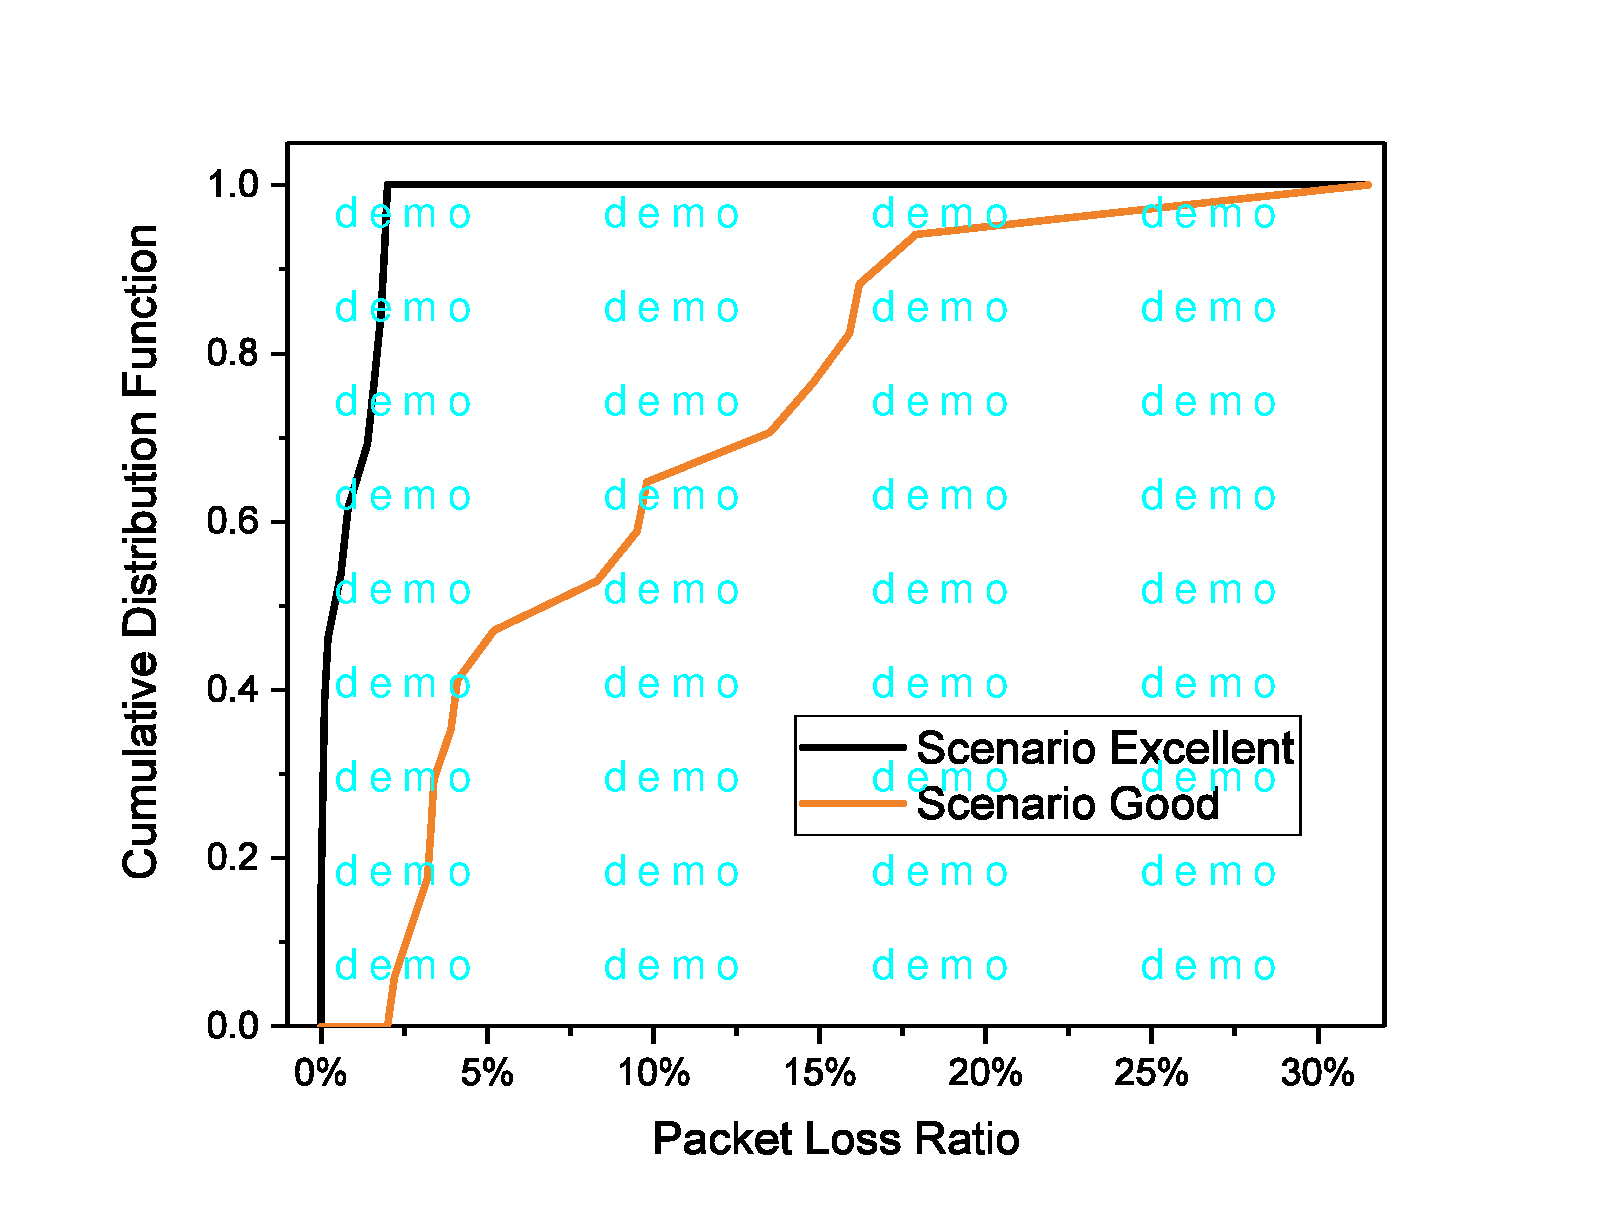
\includegraphics[width=0.7\textwidth]{chapters/chapter3/figures/capture-cdf-plr.pdf}
        \caption{两种场景平均丢包率的累积分布图}\label{fig:3:cdf-plr}
	\end{figure}
}

如图\ \nref{fig:3:cdf-plr},两种场景平均丢包率的累积分布出现偏离。Excellent场景的丢包率普遍较低,对时间隐通道的存在更敏感;Good场景中噪声干扰严重,丢包率上升,时间隐通道的检测难度增大。

\subsection{区间丢包数}
\label{chap:analyze:results:window}

\insertFigure{
	\begin{figure}[htbp]
		\centering
        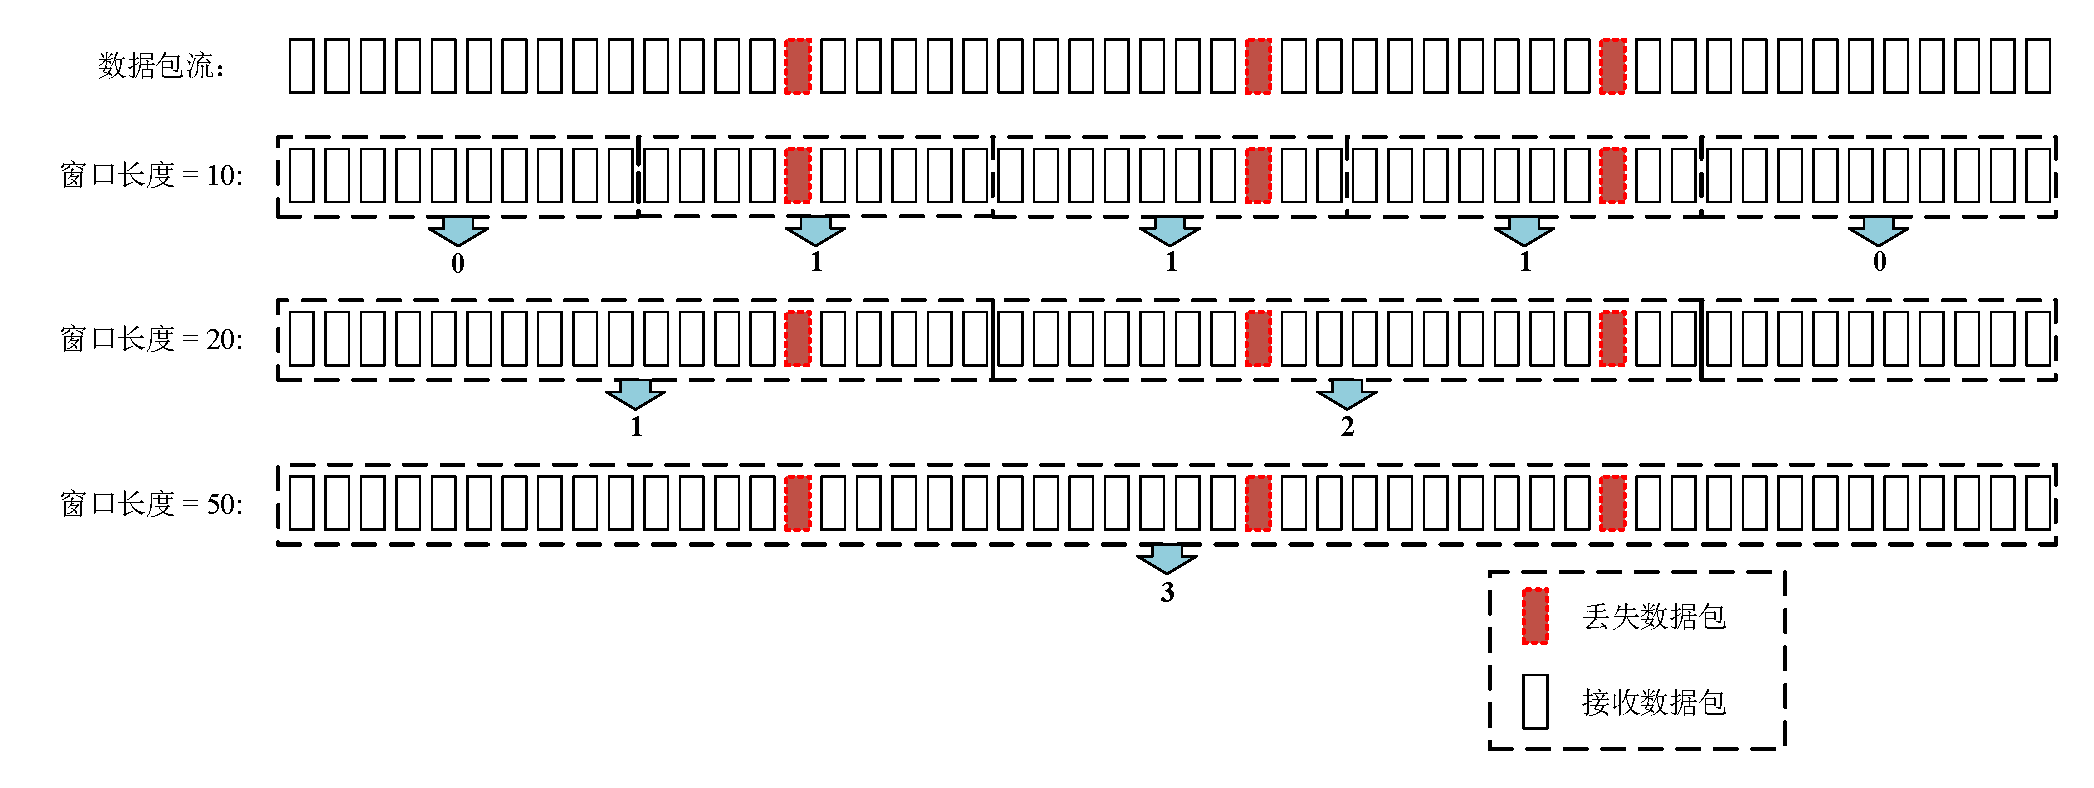
\includegraphics[width=0.99\textwidth]{chapters/chapter3/figures/win-size-count.pdf}
        \caption{区间长度与区间丢包数示意图}\label{fig:3:win-size-count}
    \end{figure}
}

%测试区间设定,以及不同场景下,各个区间的分布函数
如图\ \nref{fig:3:win-size-count},在相同丢包分布下,区间丢包数随着区间长度增大而累积。基于区间丢包数的检测方法,首先将数据包按照设定的区间长度划为独立区间,然后统计每个区间内的丢包数量。最终汇总各区间的统计结果,计算累积分布函数。

\insertFigure{
    \begin{figure}[htbp]
    \centering
        \subfigure[Excellent场景的累积分布函数]{
            \label{fig:3:capture:win-cdf:excellent}
            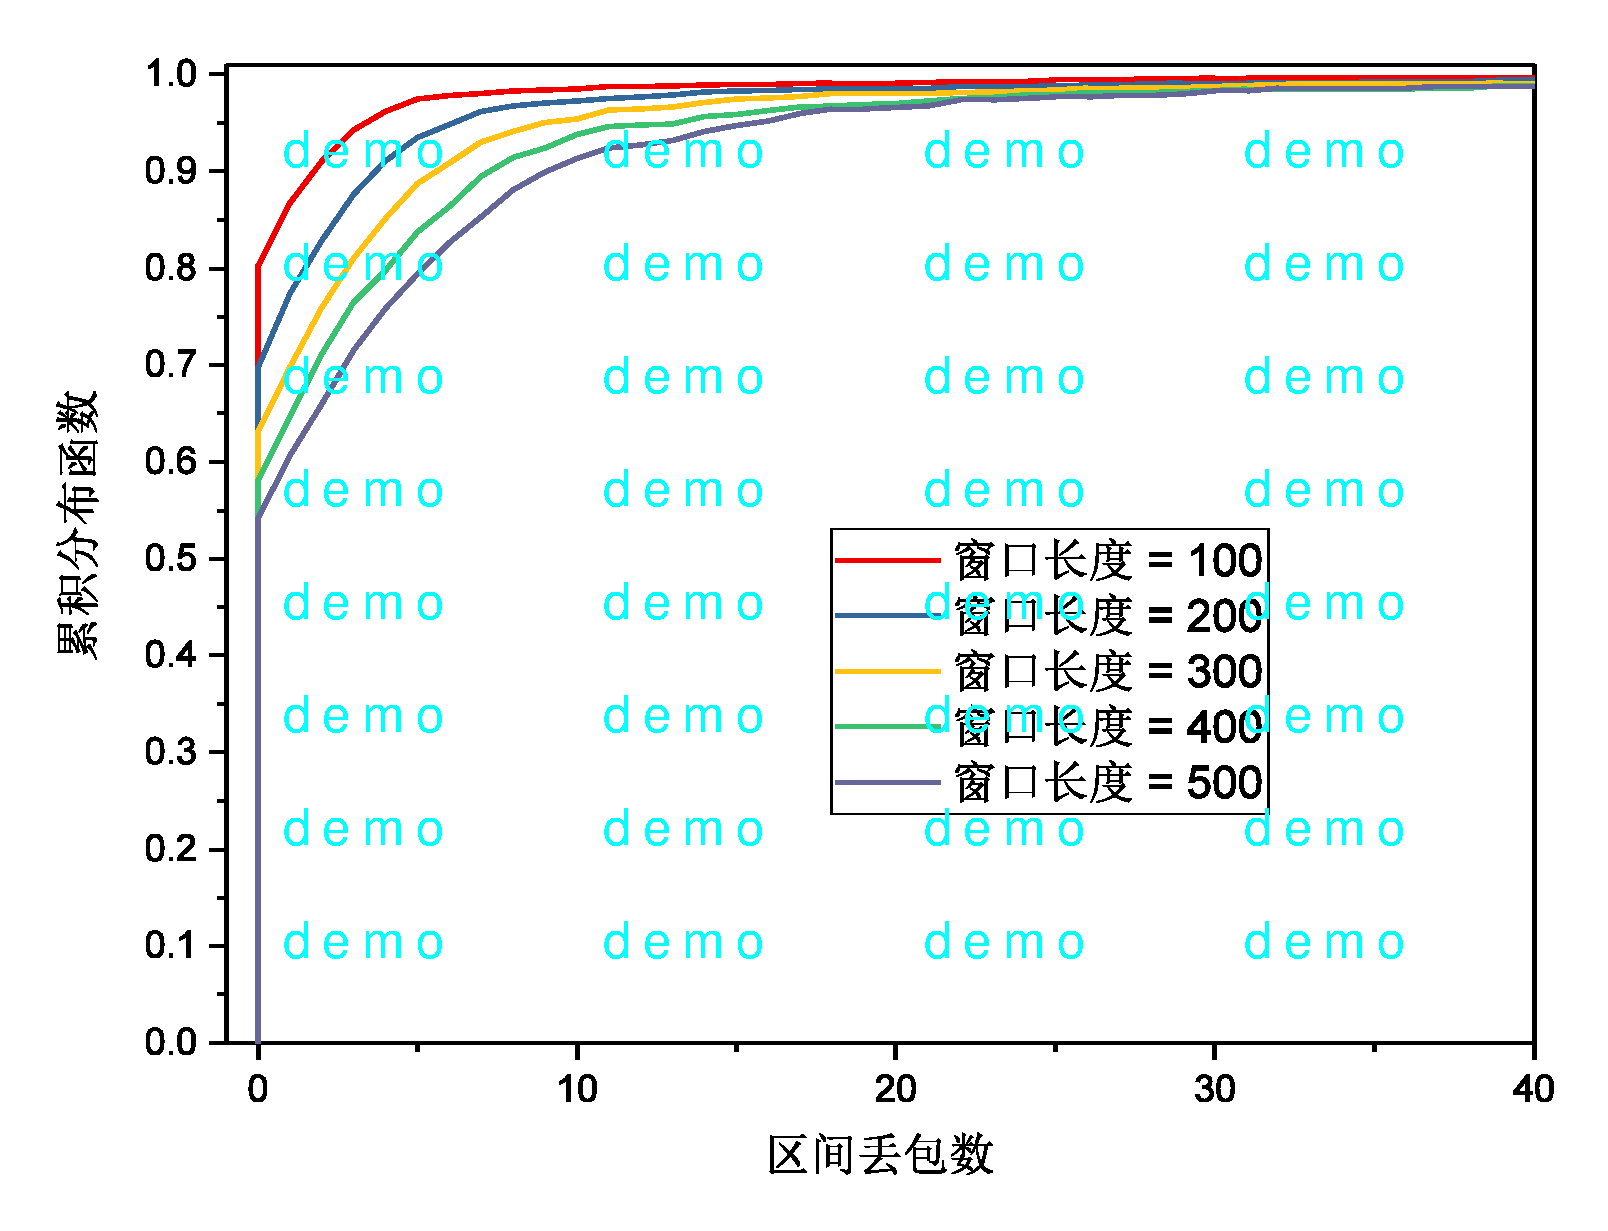
\includegraphics[width=0.48\textwidth]{chapters/chapter3/figures/capture-cdf-win-excellent.pdf}
        }
        \subfigure[Good场景的累积分布函数]{
            \label{fig:3:capture:win-cdf:good}
            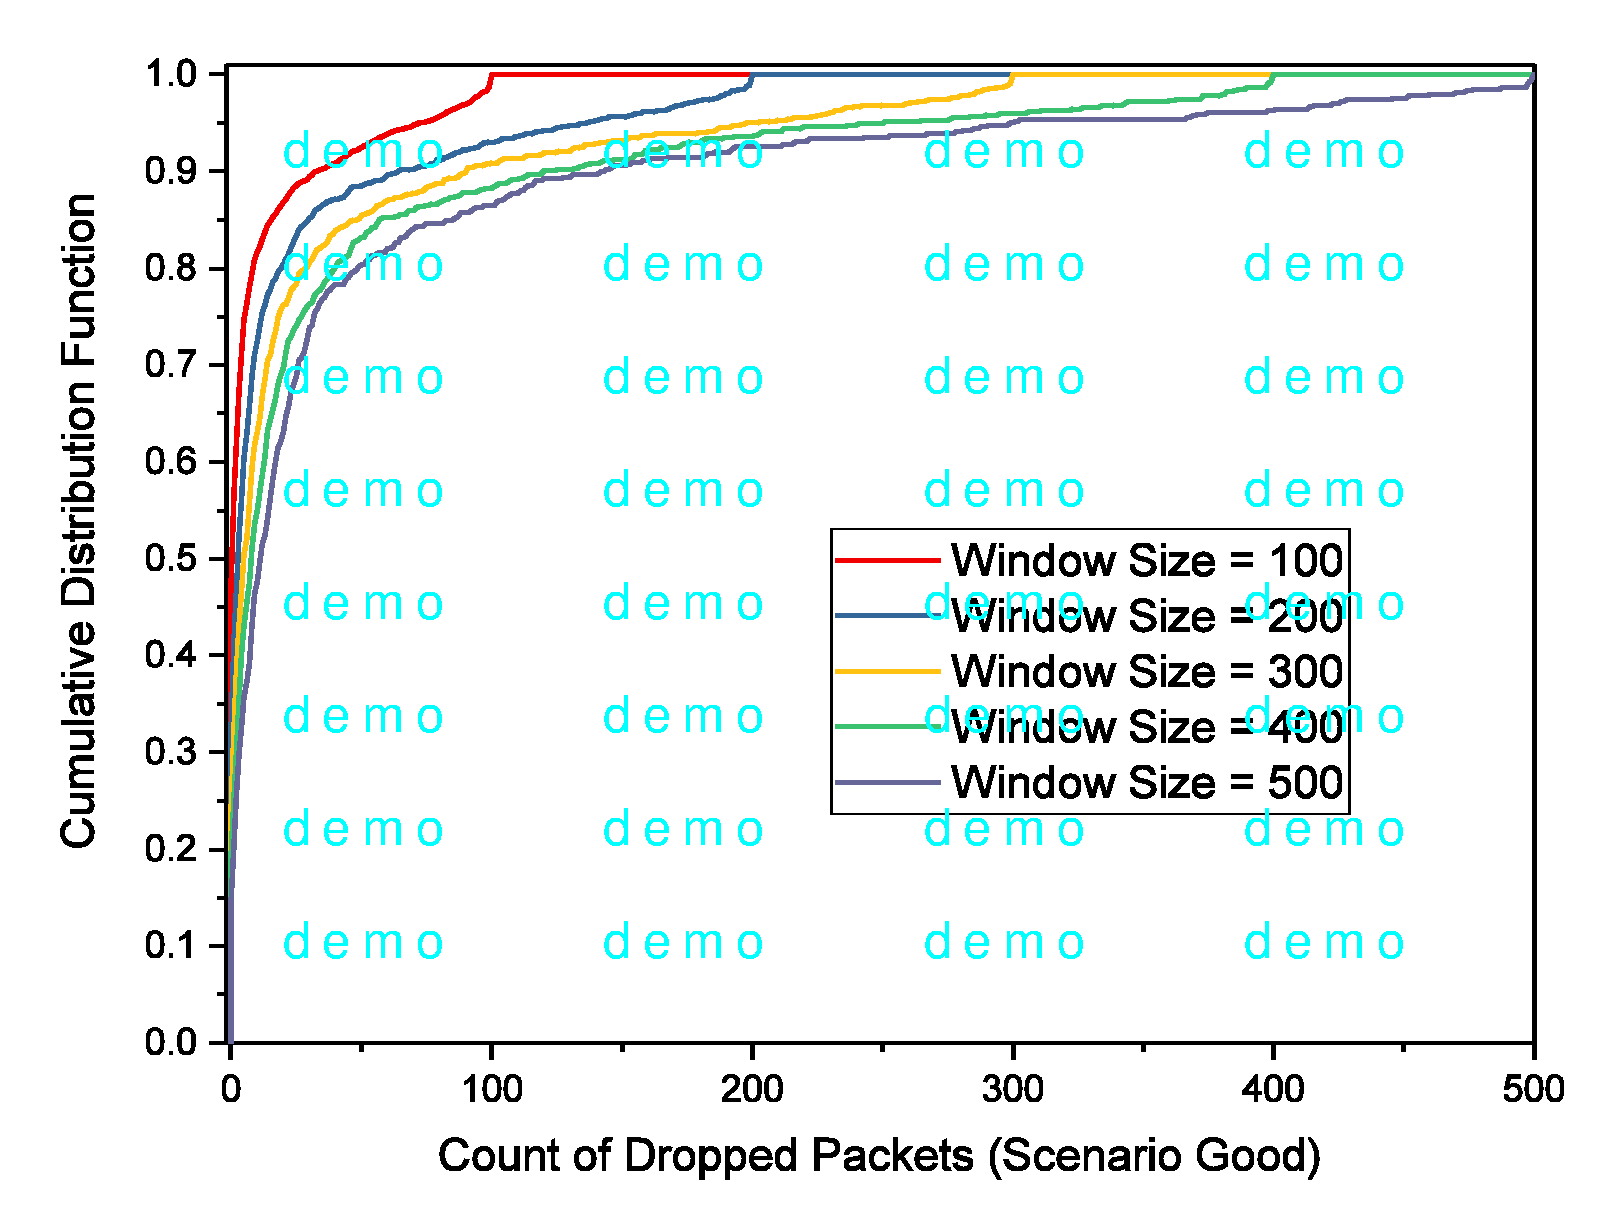
\includegraphics[width=0.48\textwidth]{chapters/chapter3/figures/capture-cdf-win-good.pdf}
        }
    \caption{区间丢包数的累积分布函数图}
    \label{fig:3:capture:win-cdf}
    \end{figure}
}

如图\ \nref{fig:3:capture:win-cdf},两种场景下的累积分布函数既存在相似性,又在存在局部差异。图\ \nref{fig:3:capture:win-cdf:excellent}中,丢包数量为$0$的区间均占据一半以上,并且CDF收敛到$1.0$的趋势较快,反应出网络质量较好。图\ \nref{fig:3:capture:win-cdf:good}中,曲线上升趋势与图\ \nref{fig:3:capture:win-cdf:excellent}类似,但丢包数量为$0$的部分比重较小,并且存在数据包全丢的区间。

\insertFigure{
    \begin{figure}[htbp]
        \centering
            \subfigure[区间长度为200时的概率质量函数]{
                \label{fig:3:capture:win-pmf:200}
                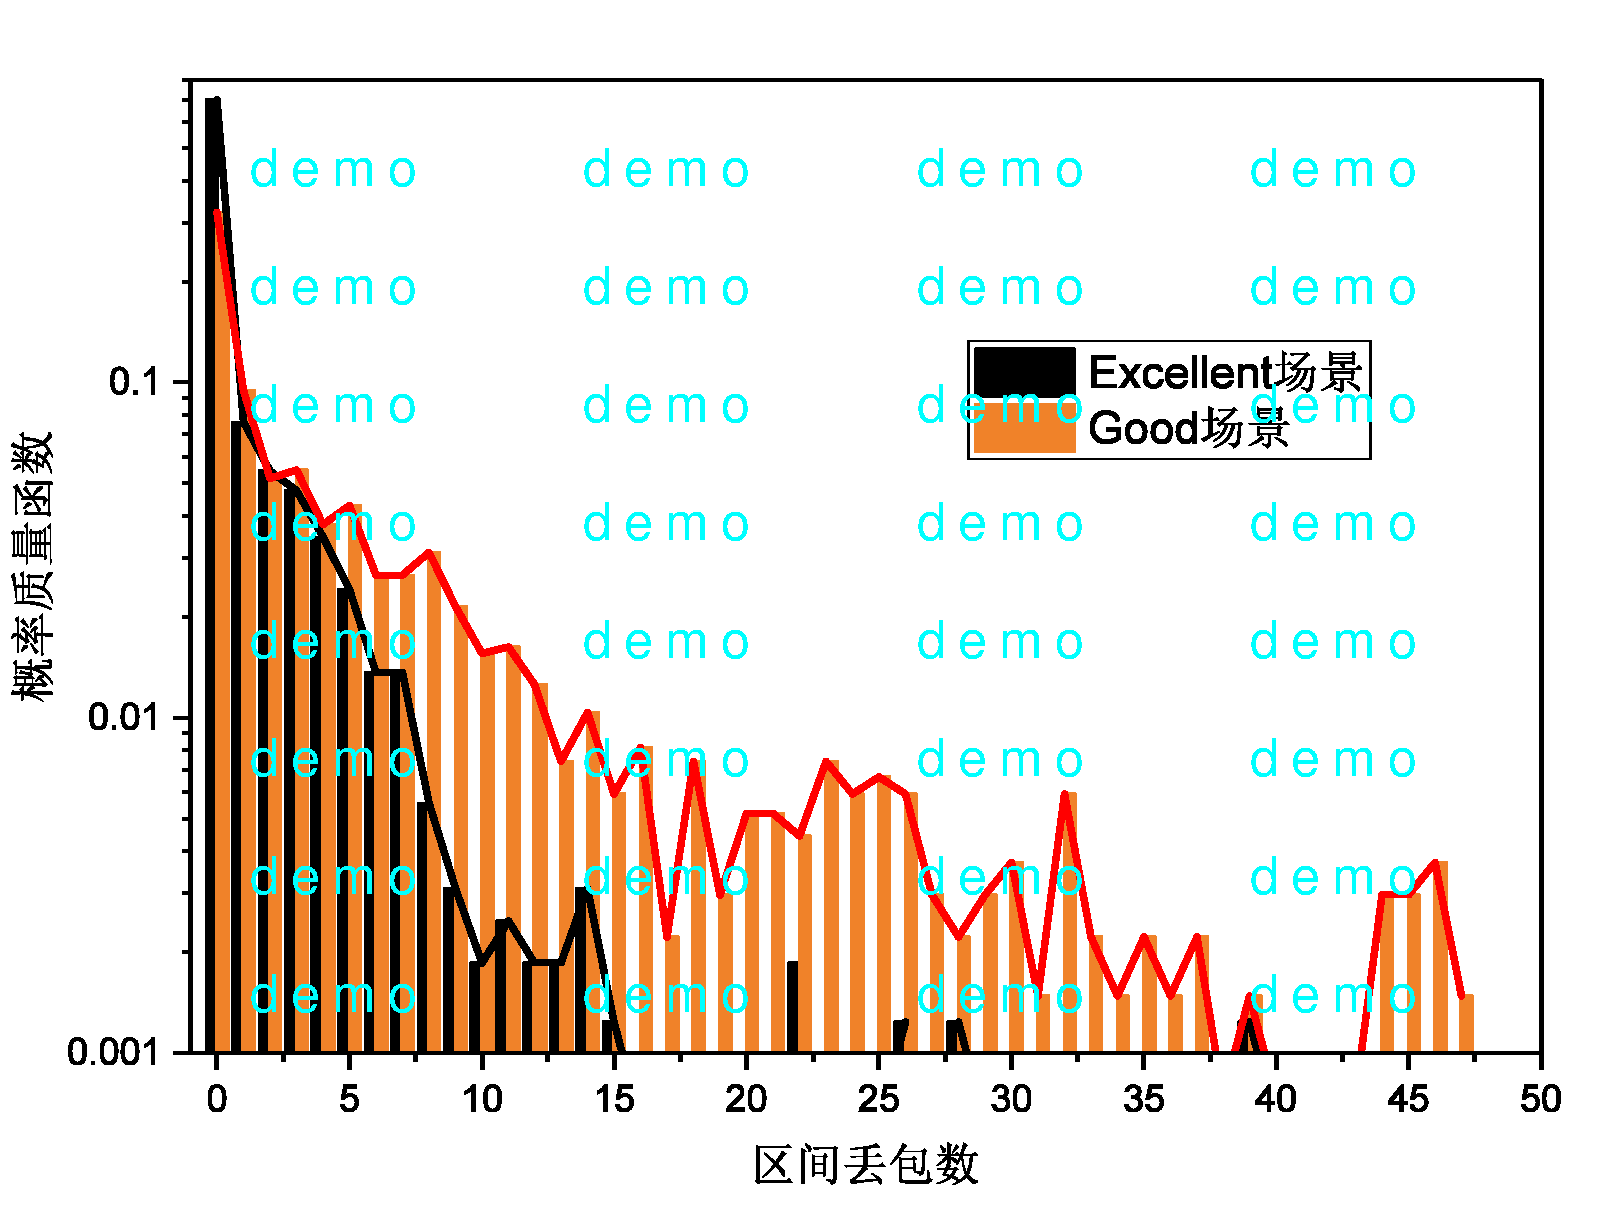
\includegraphics[width=0.48\textwidth]{chapters/chapter3/figures/capture-pmf-win200.pdf}
            }
            \subfigure[区间长度为400时的概率质量函数]{
                \label{fig:3:capture:win-pmf:400}
                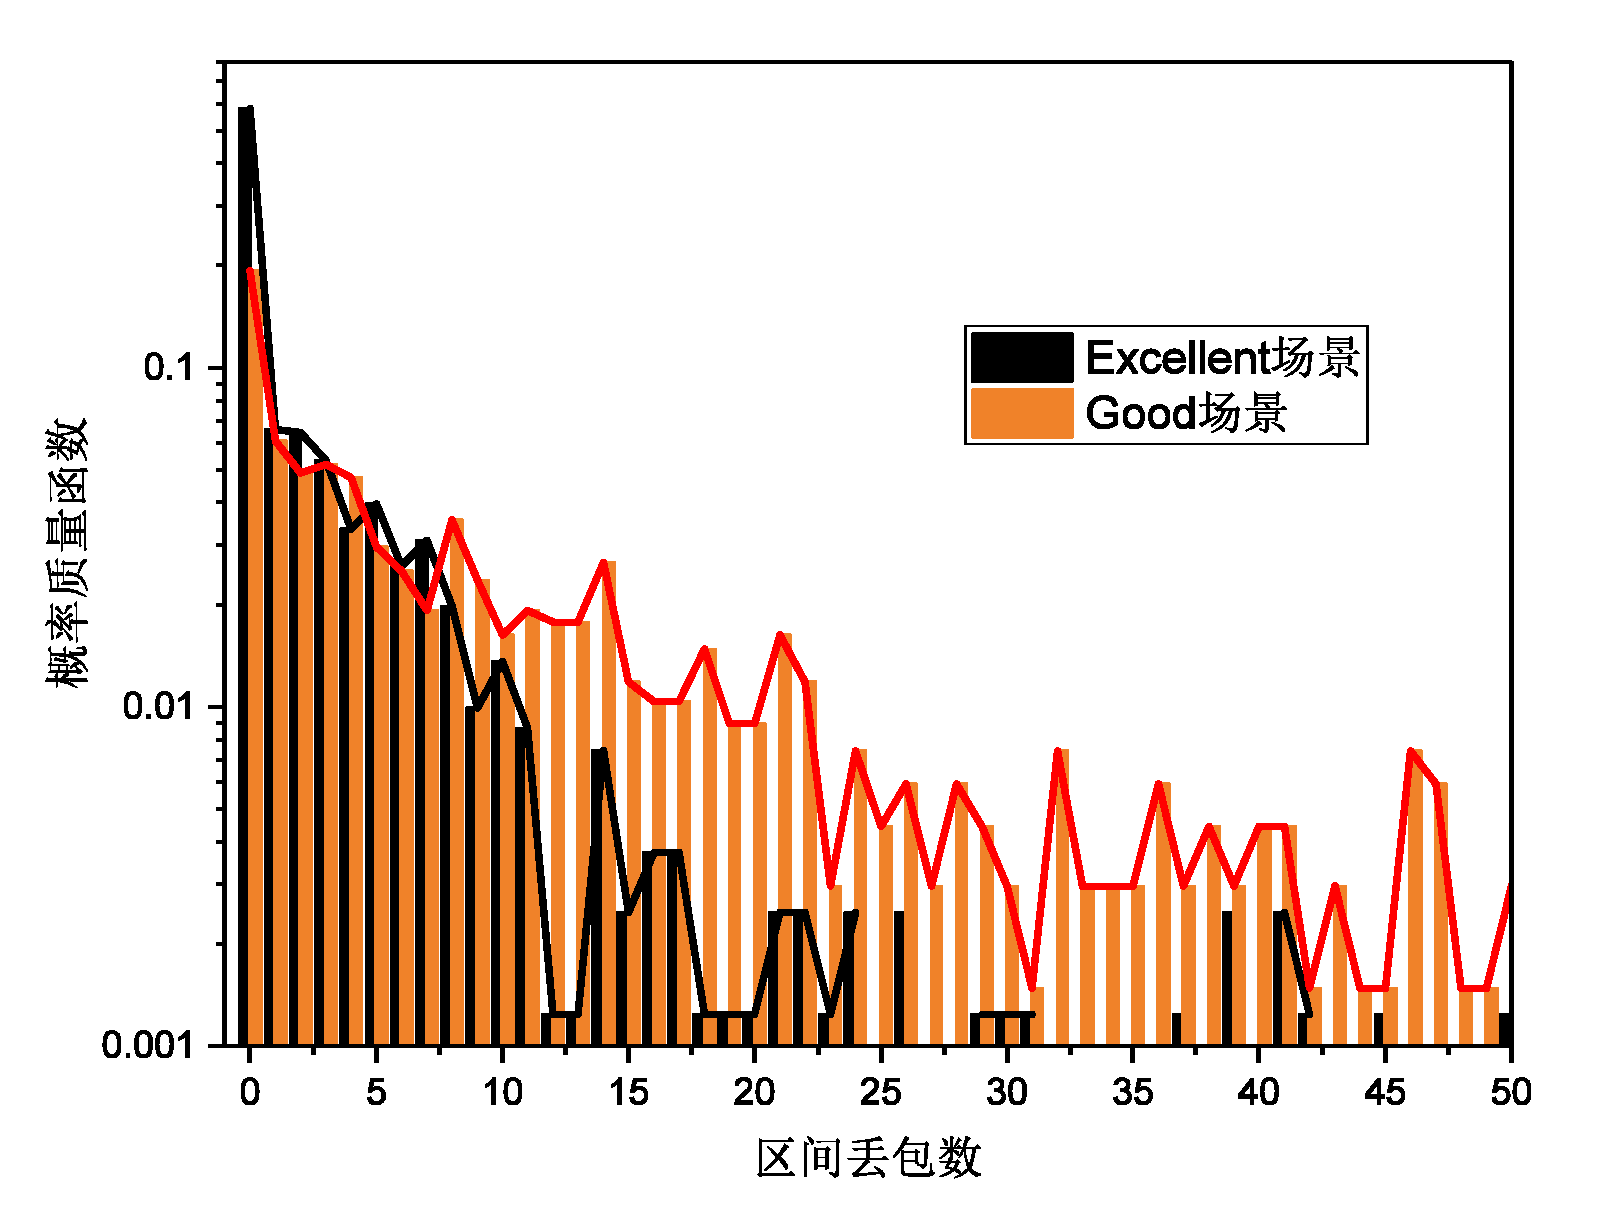
\includegraphics[width=0.48\textwidth]{chapters/chapter3/figures/capture-pmf-win400.pdf}
            }
        \caption{区间丢包数的概率质量函数图}
        \label{fig:3:capture:win-pmf}
        \end{figure}
}

如图\ \nref{fig:3:capture:win-pmf},概率质量函数在不同的场景中存在差异。概率质量函数存在不连续现象,并且不同场景中趋势差距较大,因此对区间丢包数的检验需要从整体的角度进行。

\subsection{数据包传输间隔}
\label{chap:analyze:results:ipd}

%IPD代表了什么
IPD是时间隐通道的基本检测对象,如图\ \nref{fig:2:cdf-ipd},发送与接收阶段的IPD分布存在差异。发送阶段存在两个聚集区间,而接收阶段曲线趋于平滑,证明网络缓冲及数据包转发削弱了原始IPD特征,导致接收方观测到的IPD接近正偏态分布。

%两种场景下抓包得到的IPD分布
\insertFigure{
    \begin{figure}[htbp]
    \centering
        \subfigure[IPD分布的累积分布函数图]{
            \label{fig:3:capture:ipd:cdf}
            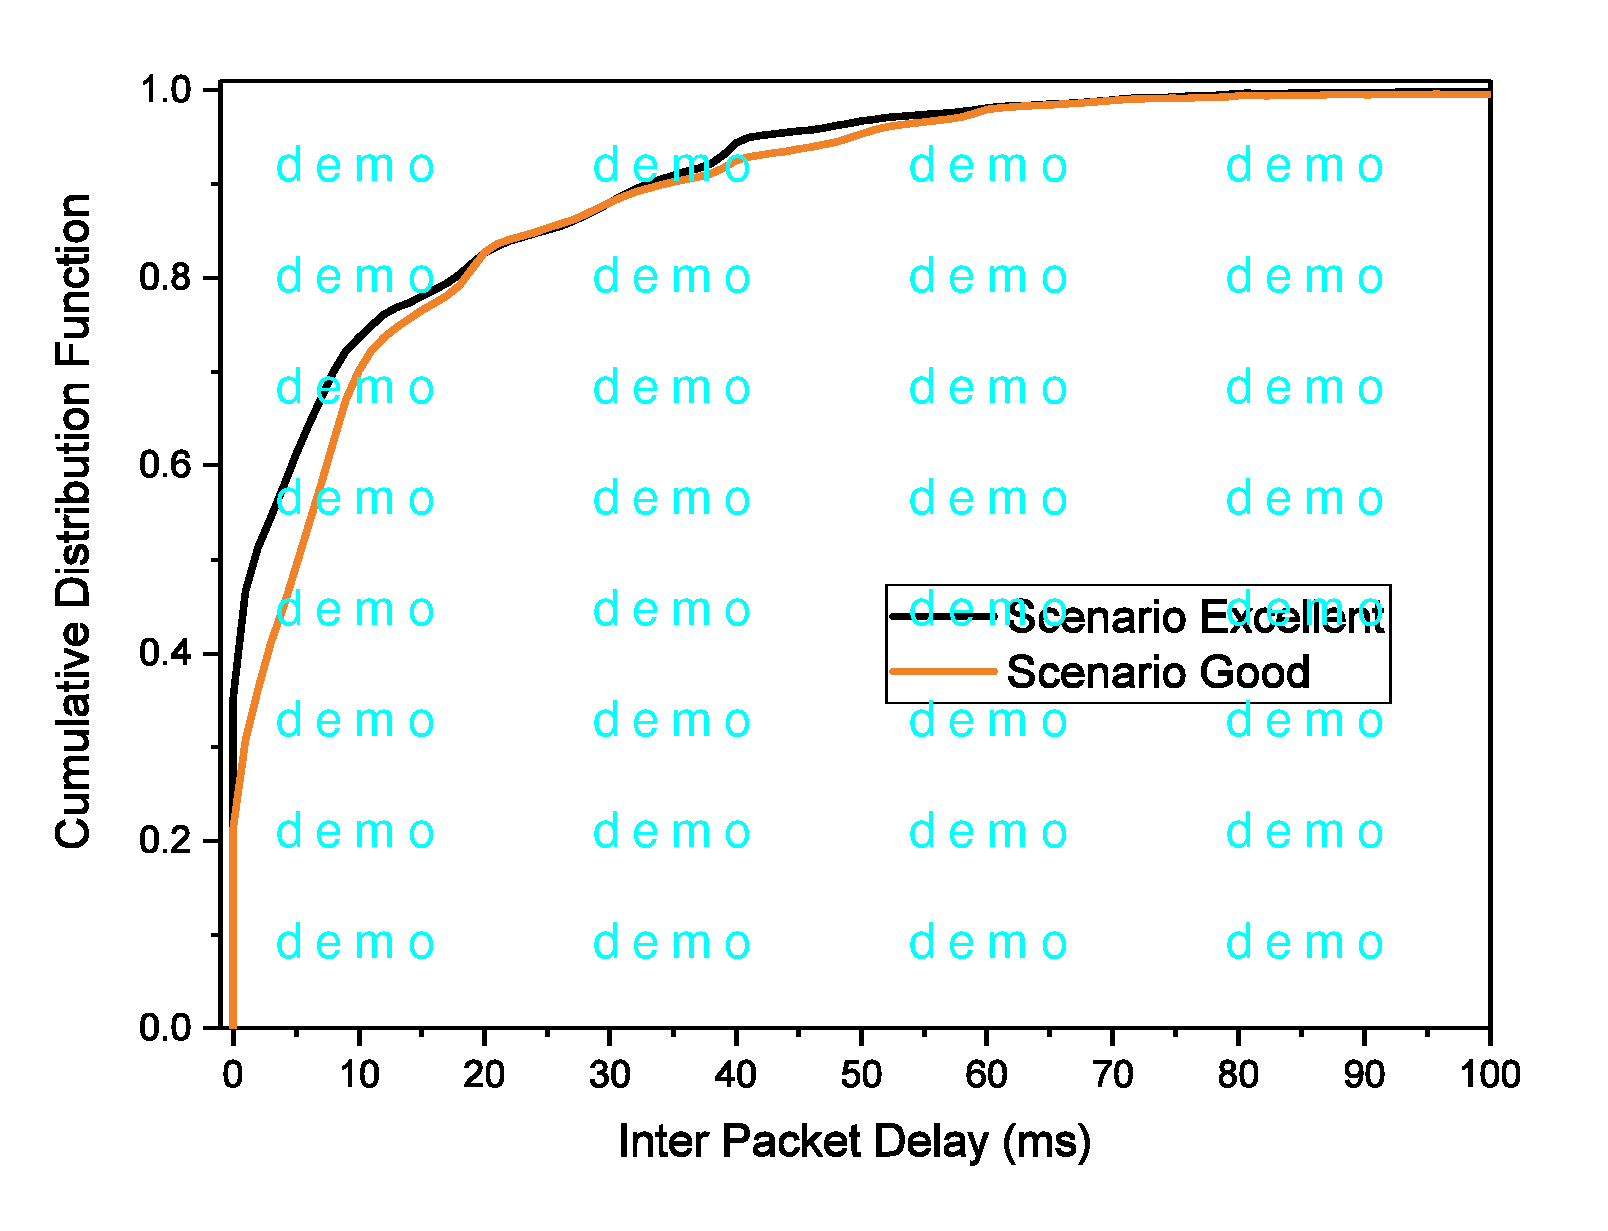
\includegraphics[width=0.48\textwidth]{chapters/chapter3/figures/capture-ipd-cdf.pdf}
        }
        \subfigure[IPD分布的概率质量函数图]{
            \label{fig:3:capture:ipd:pmf}
            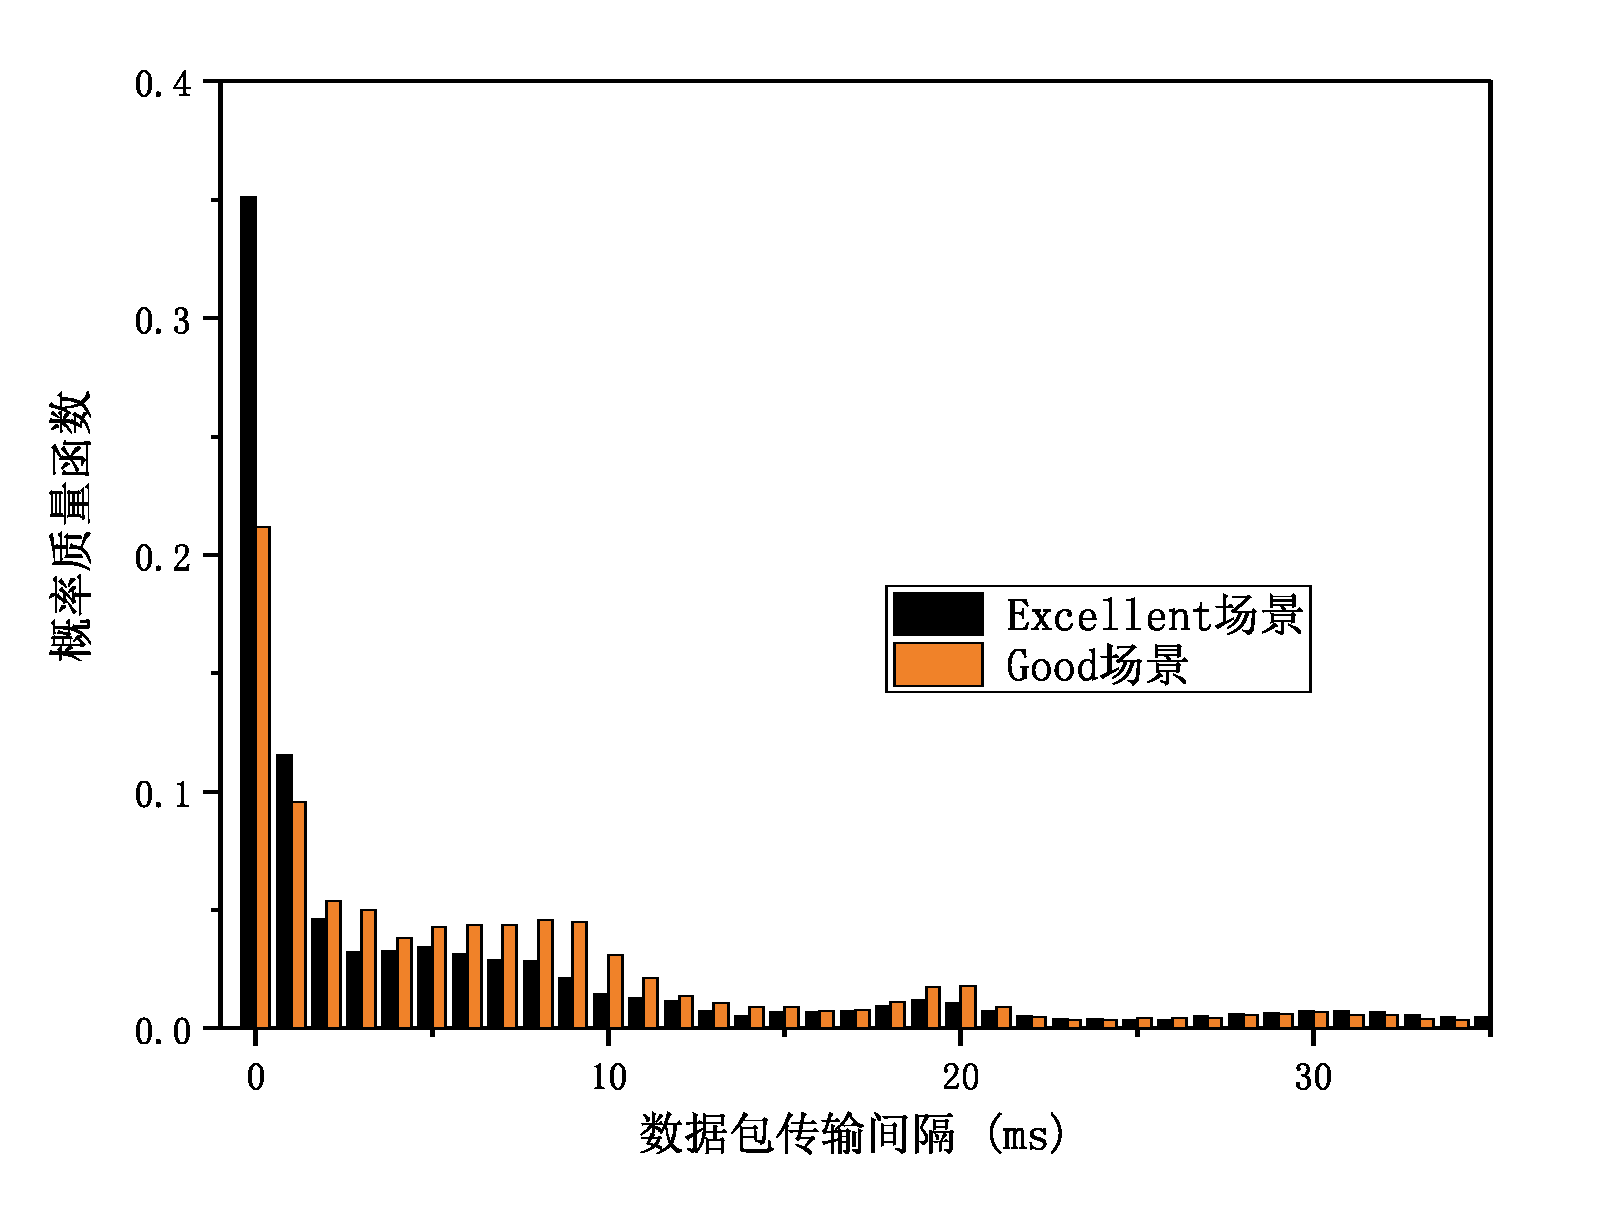
\includegraphics[width=0.48\textwidth]{chapters/chapter3/figures/capture-ipd-pmf.pdf}
        }
    \caption{VoLTE视频数据包IPD分布图}
    \label{fig:3:capture:ipd}
    \end{figure}
}

图\ \nref{fig:3:capture:ipd}中,分别展示了两种场景下的IPD分布情况。如图\ \nref{fig:3:capture:ipd:cdf},两种场景中的趋势及数值范围均近似,证明丢包事件对IPD分布的影响较小。图\ \nref{fig:3:capture:ipd:pmf}中,IPD的概率质量函数在不同场景中也具有近似的趋势。综合概率质量函数及累积分布函数的变化趋势,对于基于主动丢包的时间隐通道,仅通过IPD分布进行检测是不完善的。另一方面,证明了基于主动丢包的时间隐通道构建方法,在当前检测方法面前具有较好的隐蔽性。

\subsection{连续丢包}
\label{chap:analyze:results:burst}

%什么是连续丢包数
网络中的丢包事件,通常分为随机丢包和一定长度的连续丢包\nupcite{816237,6711984}。对于视频通话,随机丢包持续影响视频质量,连续丢包主要影响通话稳定性\nupcite{5977359,6894614,1709847}。本文中,将随机丢包作为连续丢包的一种特殊情况,即长度为1的连续丢包,在统计中统一处理。

%两种场景下,测试得到的连续丢包数信息
\insertFigure{
    \begin{figure}[htbp]
        \centering
            \subfigure[连续丢包数的累积分布函数图]{
                \label{fig:3:capture:burst:cdf}
                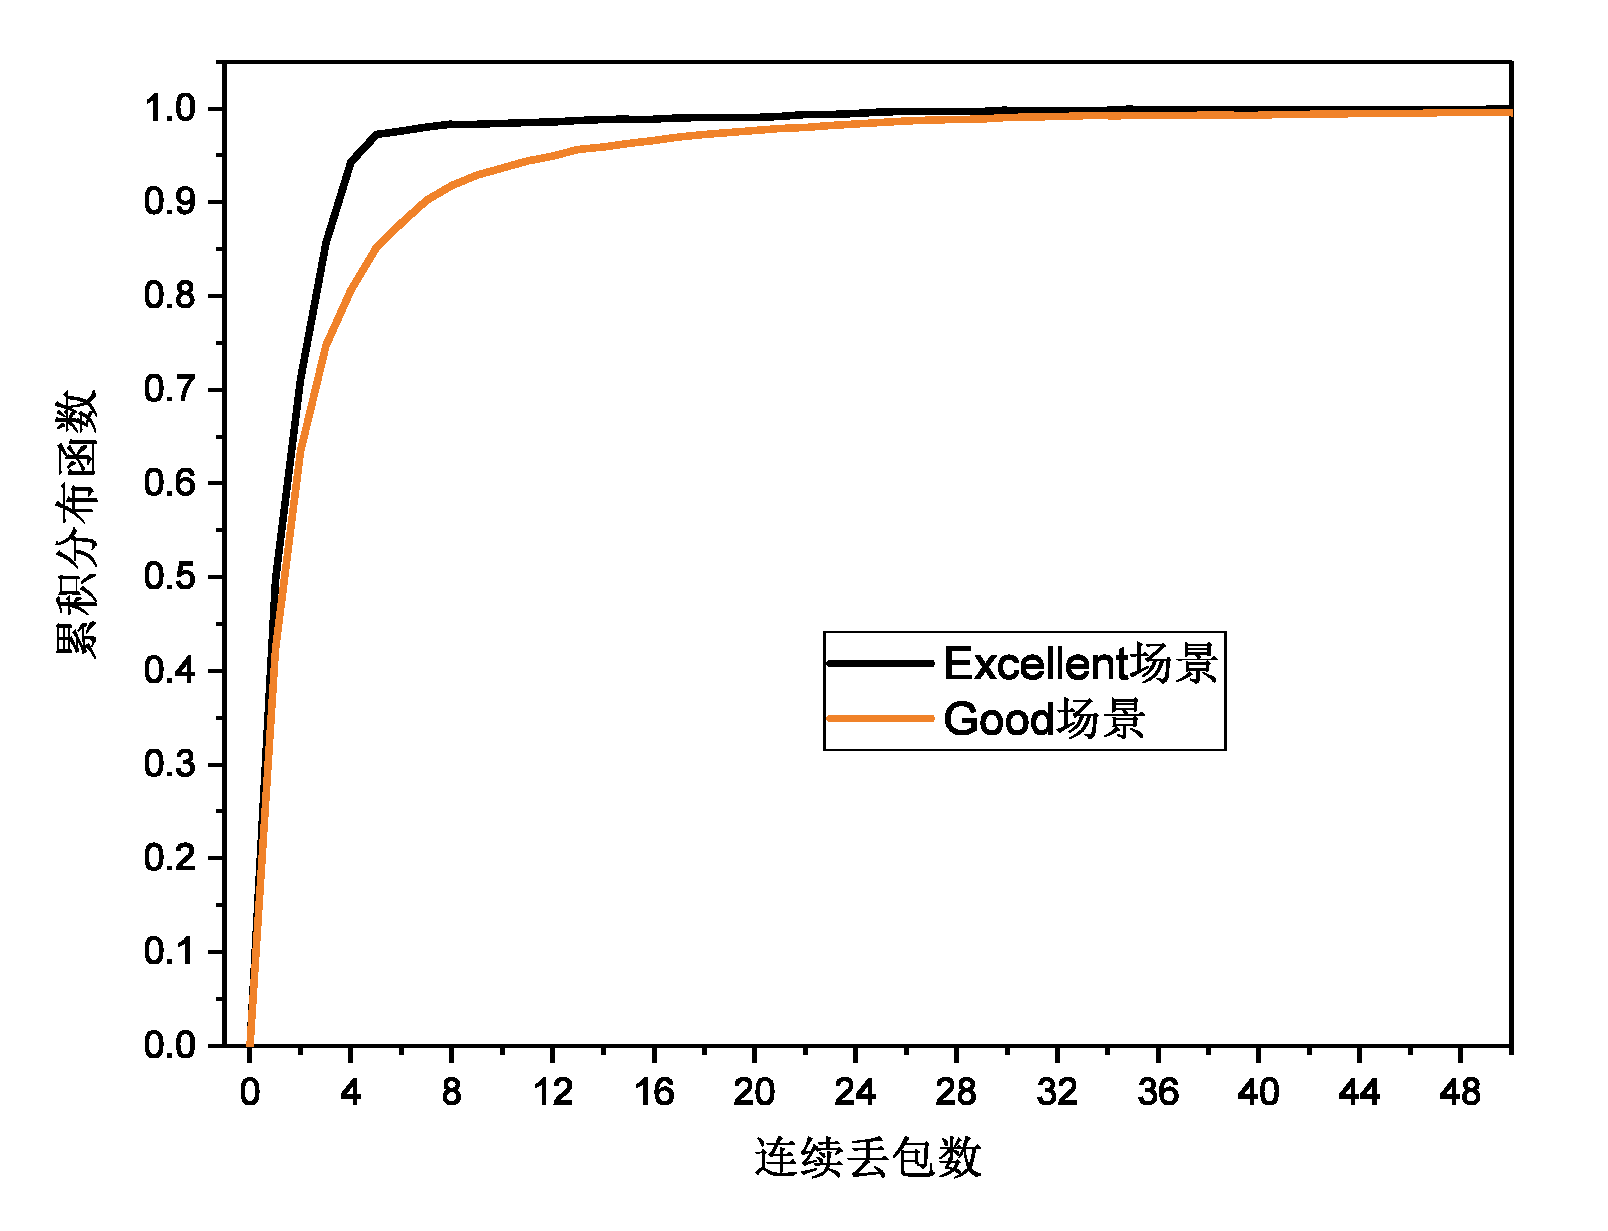
\includegraphics[width=0.48\textwidth]{chapters/chapter3/figures/capture-cdf-burst.pdf}
            }
            \subfigure[连续丢包数的概率质量函数图]{
                \label{fig:3:capture:burst:pmf}
                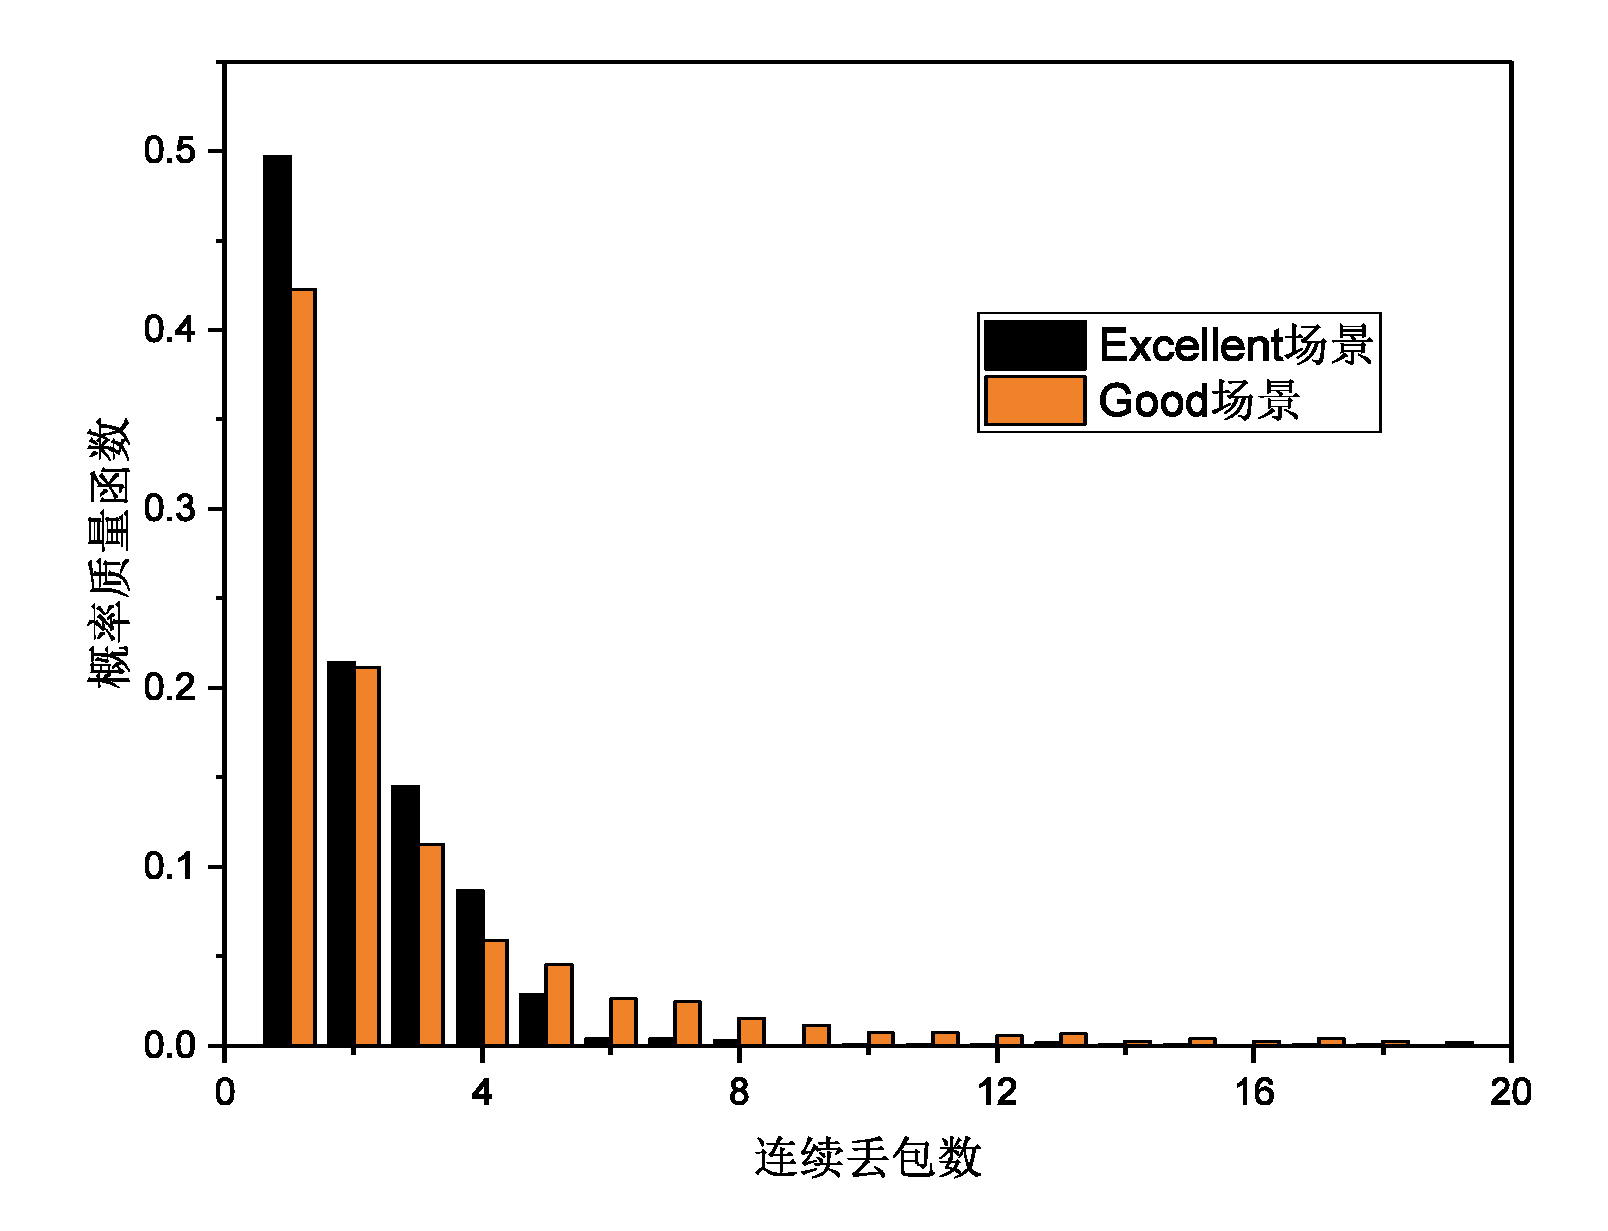
\includegraphics[width=0.48\textwidth]{chapters/chapter3/figures/capture-pmf-burst.pdf}
            }
        \caption{两种场景中连续丢包数的分布图}
        \label{fig:3:capture:burst}
    \end{figure}
}

如图\ \nref{fig:3:capture:burst},两种网络场景中,连续丢包数的分布趋势趋于一致。然而局部特征方面,Excellent场景与Good场景在连续丢包数大于1的部分,在总体中的占比存在差异。如图\ \nref{fig:3:capture:burst:cdf},Excellent场景中,连续丢包数普遍较小,累积分布函数曲线在起始阶段上升迅速;Good场景中,连续丢包导致CDF曲线趋近1的速度减缓。如图\ \nref{fig:3:capture:burst:pmf},连续丢包数的概率质量函数具有规律,并且分布曲线平滑连续。基于主动丢包的时间隐通道,导致长度为1的连续丢包增多,对分布曲线的趋势及数值存在影响。
\section{面向基于主动丢包的VoLTE时间隐通道检测方法设计}
\label{chap:analyze:statistical}

本节主要介绍,在该时间隐通道中采用的检测工具,及各种检测工具及检测对象的组合设计。在进行检测前,利用抓包得到的结果,构建标准参照,涵盖的对象包括IPD、突发丢包长度及区间丢包数量的累积分布函数及概率质量函数。对于测试样本,同样计算其累积分布函数及概率质量函数结果,通过各种检测算法,比较分布之间的差异,得出隐通道检测结论。

\subsection{基于累积分布函数的检测方法设计}
\label{chap:analyze:statistical:cdf}

%CDF函数的定义
CDF的全程是Cumulative Distribution Function,也就是累积分布函数。其统计意义,为$F_{X}(x)=P (X\leq x)$,即$X\leq x$的概率。在实际应用中,CDF的作用是分析分布的变化趋势,从而判断是否存在异常点。对于离散变量,$F_{X}(x)$的计算方式如公式(\nref{equ:3:cdf})。本方法的判别基础,是检测对象的统计特征,属于离散分布。

\insertEquation{
    \begin{equation}
    \label{equ:3:cdf}
		F_{X}(x)=\sum_{-\infty}^{x}f(x)
	\end{equation}
}

%CDF函数代表了什么
如图\nref{fig:3:capture:ipd},图\nref{fig:3:capture:ipd:pmf}的频率分布存在波动,而转换为CDF后的图\nref{fig:3:capture:win-cdf}能够更好地体现变化趋势。CDF曲线上升平缓的部分,意味着出现频率较小,所占比重较低;而CDF上升迅速的部分,对应的是PMF中占比较大的部分,也就是统计结果中频率较高的部分。

%如何通过CDF进行检测
CDF曲线是最基本的检测方法,本检测方法中,首先计算IPD、突发丢包长度及区间丢包的CDF分布。接下来,绘制分布曲线,比较曲线的趋势及起始特征,尤其是曲线之间的差值。CDF检测方法,无法直接得出量化评估结果,因此,在时间隐通道检测方法中,作为初步筛选及分析方式。进一步,在CDF统计结果的基础上,进行分布一致性检验,得到确定的检测结果。

\subsection{基于分布一致性的检测方法设计}
\label{chap:analyze:statistical:test}

%一致性检验的通用解释
对于两个独立的样本,判断其是否来自同一个分布,需要借助的统计中分布一致性检验。在理想情况下,观测值出现的频率,与分布函数中的概率是对应的,观测值的分布函数在一定程度上可以代替真实的分布函数。一致性检验首先假设两个样本属于同分布,然后统计计算观测值与合理值的取值,比较判断假设是否成立。

%一致性检验使用的对象
用于一致性检验的样本数据越多,采样结果与真实分布更接近,检验结果具有更高的可信度。在\nref{chap:analyze:results}中,介绍了几种观测对象,其中IPD的分布存在明显的规律性,且不同网络环境下的分布基本一致。因此,本检测方法主要用于检测IPD分布的一致性。

\subsubsection{基于Kolmogorov-Smirnov test的检测方法设计}
\label{chap:analyze:statistical:test:ks}

%K-S检验的数学理论
Kolmogorov-Smirnov检验是常用的无参数、双样本检验方法,检验原理基于累积分布函数。\nupcite{doi:10.1080/01621459.1951.10500769,doi:10.1080/01621459.1967.10482916}如公式\nref{equ:2:ks},K-S检验基于CDF分布中的最大差异$D_{KS}$。当置信区间设定为$95\%$时,使用公式(\nref{equ:2:ks-p})计算$D_{KS,0.05}$,当$D_{KS}<D_{KS,0.05}$时,可以认为两个样本的分布式一致的。

%K-S检验的一致性判定
在实际应用中,通常根据$D_{KS,0.05}$的分布计算$p$值,当$p\leq 0.05$时,假设成立,样本来自相同的分布。
K-S检验在大样本环境中具有较高的准确度,样本数量较少时,统计的分布存在误差,最终检验结果不具有可靠性。同样需要注意的是,当样本数据增加时,$D_{KS,0.05}$会相应减小,$D_{KS}$上限降低,当采样不均匀时,出现误判结果。
因此,本检测方法中,K-S检验用于时间隐通道构建前后,相同样本的检测。

\subsubsection{基于Welch’s t检验的检测方法设计}
\label{chap:analyze:statistical:test:t}

%T-test的数学理论
Welch’s t检验,应用于两个独立的样本,主要评估样本的平均值是否存在差异。通常应用于验证两个独立的采样结果,在方差相同的情况下,是否具有相同的平均值。当样本基本符合正态分布时,该检验方法可以判断样本分布的一致性。Welch's t检验的优势,是可以应用与样本规模不一致的场景,具有较好的鲁棒性。

\insertEquation{
    \begin{equation}
    \label{equ:3:t-value}
		t=\frac{\overline{X}_{1}-\overline{X}_{2}}{\sqrt{\frac{s_{1}^{2}}{N_{1}}+\frac{s_{2}^{2}}{N_{2}}}}
	  \end{equation}

    \begin{equation}
    \label{equ:3:v-value}
		\nu \approx \frac{({\frac{s_{1}^{2}}{N_{1}}+\frac{s_{2}^{2}}{N_{2}})^{2}}}{\frac{s_{1}^{4}}{N_{1}^{2}\nu_{1}}+\frac{s_{2}^{4}}{N_{2}^{2}\nu_{2}}}
	  \end{equation}
}

%T-test的一致性判定
如公式(\nref{equ:3:t-value}),t检验首先需要计算统计值$t$,其中$\overline{X}$表示样本的均值,$s$表示样本的标准差,$N$表示样本的规模。接下来使用Welch–Satterthwaite公式计算自由度$\nu$,如公式(\nref{equ:3:v-value})。最后,根据Student's t-分布,计算在自由度$\nu$下,统计值$t$对应的概率,即可判断样本的相似性。

类似K-S检验,Welch's t检验得到的$p$值,反映了样本的一致性水平,一般取0.05作为分界值,对应两个样本分布一致的概率为95\%。因为Welch’s t检验适用范围的限制,只有在正态分布的情况下具有较好的效果,而在\nref{chap:analyze:results}中分析可知,IPD等统计特征的分布,多为偏态分布,因此,Welch's t检验作为IPD的检验方式之一。

\subsubsection{基于Mann-Whitney rank检验的检测方法设计}
\label{chap:analyze:statistical:test:mw}

%M-W检验的数学理论
Mann–Whitney rank检验,又称为Mann–Whitney U检验或Mann–Whitney–Wilcoxon检验,应用双样本无参数检验,对应的目标分布为均匀分布。不同于Welch's t检验,Mann–Whitney rank检验的目标分布为非正态分布,适用于大数据集的检验场景。

\insertEquation{
    \begin{equation}
    \label{equ:3:u-value}
		U_{i}=R_{i}-\frac{n_{i}(n_{i}+1)}{2}
	\end{equation}
}

%M-W检验的一致性判定
Mann–Whitney rank检验过程中,首先要将样本混合,然后按照顺序,为每个样本值分配排名。接下来,分别计算两个样本中的排名之和$R_{1}$及$R_{2}$。根据公式(\nref{equ:3:u-value}),分别计算两个样本的$U_{1}$及$U_{2}$,并取$U=min(U_{1},U_{2})$与$U_{0.05}$进行比较,当$U>U_{0.05}$时,即可认定样本属于同分布。

Mann–Whitney rank检验作为Welch's t检验的补充,应用于不满足正态分布的检验场景,关注的重点,是样本均值的偏离程度。因此,Mann–Whitney rank与Welch's t检验组合,作为IPD的一致性检验方法。

\insertTable{
	\begin{table}[]
        \centering
        \caption{分布一致性检测方法的适用范围}
        \label{tab:3:test-range}
        \begin{threeparttable}
            \begin{tabular*}{0.99\textwidth}{@{\extracolsep{\fill}}ccc}
              \toprule
              检验方法 & 测试对象 & 通过条件\\ 
              \midrule
              K-S检验 & IPD分布 & 隐通道构造前后,p值满足$p>0.05$ \\ 
              Welch's t检验 & IPD分布 & 同一场景下的样本,p值满足$p>0.05$ \\ 
              Mann–Whitney rank检验 & IPD分布 & 同一场景下的样本,p值满足$p>0.05$ \\ 
              \bottomrule
            \end{tabular*}
            \begin{tablenotes}
              \footnotesize
              \item[] Welch's t检验与Mann–Whitney rank检验通过一种即可
          \end{tablenotes}
        \end{threeparttable}
    \end{table}
}

如表\nref{tab:3:test-range},根据一致性检验方法的特征,及VoLTE中基于主动丢包的时间隐通道检测需求,不同的检验方法的测试通过条件存在差异。K-S检验作为独立的检验方式,验证的是IPD分布在时间隐通道构建前后的一致性。Welch's t检验及Mann–Whitney rank检验,作为互相补充的组合,共同检验同一场景下,样本与一致分布的差异,并且两种检验方法通过一种即可认定一致。

\subsection{基于熵的检测方法设计}
\label{chap:analyze:statistical:entropy}

%熵的数学意义是什么
基于熵的检测方法,主要依赖条件熵中的Kullback-Leibler散度。\nupcite{5590253,Gianvecchio:2007:DCT:1315245.1315284}K-L散度的计算方法,如公式(\nref{equ:2:kld}),$G(x)$作为参照分布,$F(x)$作为样本分布,二者在关系上具有约束。同时,K-L散度计算中,要求所有的输入概率值非0。

%如何通过熵判定一致性
基于熵的检测方法,优势在于对检测样本的实际分布不敏感,可以应用于任意类型的测试场景中。根据系统的熵增原理,不同的分布之间一定存在熵值差异,通常约定K-L散度值0.1作为分界线,当K-L散度超过0.1时,可以认为分布之间存在明显差异,不属于同分布。

\insertTable{
	\begin{table}[]
      \centering
      \caption{基于熵的检测方法适用范围}
      \label{tab:3:entropy-range}
          \begin{tabular*}{0.7\textwidth}{@{\extracolsep{\fill}}ccc}
            \toprule
            检验方法 & 测试对象 & 通过条件 \\ 
            \midrule
            \multirow{3}{*}{K-L散度} & IPD分布 & \multirow{3}{*}{K-L散度$<0.1$} \\ 
            & 突发丢包长度分布 \\
            & 区间丢包分布 \\
            \bottomrule
          \end{tabular*}
    \end{table}
}

如表\nref{tab:3:entropy-range},K-L散度检测可以应用于所有的观测特征,并且判别标准都是相同的。在实际的测试中,K-L散度结果的数量级与样本分布密切相关,因此具有非常好的灵敏度。

\subsection{基于相对距离的检测方法设计}
\label{chap:analyze:statistical:distance}

%相对距离的通用解释
相对距离体现了分布变化所需要的代价,传统意义上的距离表示的是空间上的度量,统计学中借鉴这一思想,用相对距离来度量样本分布改变为参照分布所需要的成本。
%相对距离的检验对象
相对距离的检测对象,适用于具有参照样本的双样本检测,重点关注样本与参照之间的差异程度。

\subsubsection{Wasserstein距离}
\label{chap:analyze:statistical:distance:wasserstein}

%wasserstein距离的数学理论
Wasserstein距离又称为空间传输距离,作为无参数检测方法,其评估对象是一个分布转换为另一个分布所需要的的代价。\nupcite{ramdas2015wasserstein}参照运输过程中的最小能量消耗,计算过程中需要同时考虑移动的分量及距离,最终计算总代价,反映了两个分布之间的相对距离。

\insertEquation{
    \begin{equation}
    \label{equ:3:wasserstein-distance}
		D_{w}(F(x),G(x)) = \sum{\frac{|F(x)-G(x)|}{n}}
	\end{equation}
}

%相对距离的一致性判定
在通常的计算方法中,Wasserstein距离中的每个样本点都有其权重,本检测方法中测试的是分布曲线之间的相对距离,因此设定曲线中的每个样本点都具有相同的权重。计算方式如公式(\nref{equ:3:wasserstein-distance}),其中,$F(x)$及$G(x)$对应CDF统计结果。考虑到不同场景中,$n$的取值存在差异,为统一评估标准,Wasserstein距离评估的结果为$D_{w}(F(x),G(x))\times n$。

\subsubsection{能量距离}
\label{chap:analyze:statistical:distance:energy}

能量距离是一种评估随机向量之间距离的指标,只有当两个分布完全一致时,能量距离的取值才取0。作为一种统计工具,能量距离可以用于评估样本及假设分布的距离,也可以用于评估两个独立样本之间的距离。在独立性测试、匹配度测试、无参数测试及分类划分领域,具有普遍应用能力。\nupcite{10.1002/wics.1375}

%能量距离的数学理论
\insertEquation{
    \begin{equation}
    \label{equ:3:energy-distance}
		D_{e}(F(x),G(x))=\sqrt{2\sum{(F(x)-G(x))}^{2}}
	\end{equation}
}

能量距离的计算方式如公式(\nref{equ:3:energy-distance}),在该检测方法中,评估的是分布的相似性,因此各点权值相等,$D_{e}(F(x),G(x))$代表了CDF曲线之间距离的量化评估结果。

%相对距离的一致性判定
\insertTable{
	\begin{table}[]
      \centering
      \caption{基于相对距离的检测方法适用范围}
      \label{tab:3:distance-range}
          \begin{tabular*}{0.8\textwidth}{@{\extracolsep{\fill}}ccc}
            \toprule
            检验方法 & 测试对象 & 通过条件 \\ 
            \midrule
            \multirow{3}{*}{Wasserstein距离} & IPD分布 & \multirow{3}{*}{$D_{w}(F(x),G(x))\times n<1.5$} \\ 
            & 突发丢包长度分布 \\
            & 区间丢包分布 \\
            \\
            \multirow{3}{*}{能量距离} & IPD分布 & \multirow{3}{*}{$D_{e}(F(x),G(x))<1.5$} \\ 
            & 突发丢包长度分布 \\
            & 区间丢包分布 \\
            \bottomrule
          \end{tabular*}
    \end{table}
}

基于相对距离的检测方法,适用的测试对象及通过条件,如表\nref{tab:3:distance-range}。通常$D_{w}(F(x),G(x))\times n$及$D_{e}(F(x),G(x))$与一致性概率无关,在本检测方法中,设定上限为$1.5$,如果距离计算结果超过1.5,则认定分布不一致。

\subsection{检测方法总结}
\label{chap:analyze:statistical:sum}
该时间隐通道检测方法,综合了集中不同检测原理的判别方式,并对观测到的多种特征分布进行检验。相较单一的检测方式,对基于主动丢包的时间隐通道具有更好的检测能力。检验方法与测试对象的对应关系,如表\nref{tab:3:detect-sum}所示,共14条测试子项,当通过其中的11条量化测试方法时,可以认定不存在时间隐通道;CDF检验结果存在主观差异,作为最终结论的参照。

\insertTable{
	\begin{table}[]
      \centering
      \caption{VoLTE时间隐通道检测方法汇总}
      \label{tab:3:detect-sum}
          \begin{tabular*}{0.98\textwidth}{@{\extracolsep{\fill}}cccc}
            \toprule
            编号 & 测试对象 & 检验方法 & 通过条件 \\ 
            \midrule
            1 & \multirow{6}{*}{IPD分布} & CDF检验 & 趋势基本一致 \\ 
            2 & & K-S检验 & $p>0.05$ \\
            3 & & Welch's t检验,Mann–Whitney rank检验 & 存在$p>0.05$\\
            4 & & K-L散度 & $K-L散度<0.1$ \\
            5 & & Wasserstein距离 & $d<1.5$ \\
            6 & & 能量距离 & $d<1.5$ \\
            \\
            7 & \multirow{3}{*}{突发丢包长度分布} & CDF检验 & 趋势基本一致\\ 
            8 & & K-L散度 & $K-L散度<0.1$ \\
            9 & & Wasserstein距离 & $d<1.5$ \\
            10 & & 能量距离 & $d<1.5$ \\
            \\
            11 & \multirow{3}{*}{区间丢包数分布} & CDF检验 & 趋势基本一致\\ 
            12 & & K-L散度 & $K-L散度<0.1$ \\
            13 & & Wasserstein距离 & $d<1.5$ \\
            14 & & 能量距离 & $d<1.5$ \\
            \bottomrule
          \end{tabular*}
    \end{table}
}

\section{主动丢包时间隐通道检测方法评估}
\label{chap:analyze:result}

%本节讲述的内容,对提出的测试方法,进行检验
本文\ \nref{chap:analyze:statistical}中,提出了VoLTE主动丢包时间隐通道的检测方法,本节通过实验评估该检测方法的检测能力。基于抓包得到的测试数据集,通过模拟时间隐通道的传输行为,以检测结果验证其是否有效。

\subsection{评估方法概述}
\label{chap:analyze:result:abstract}

%测试的数据集
如表\ \nref{tab:3:capture-results}所示,抓包结果包括两种场景,测试过程也按照场景分别进行。

\insertTable{
	\begin{table}[htbp]
    \centering
    \caption{测试环境信息表}
    \label{tab:3:result:environment}
        \begin{tabular*}{0.9\textwidth}{@{\extracolsep{\fill}}cl}
            \toprule
            类型 & 详细信息 \\
            \midrule
            PC平台 & i5-9400,DDR4 16GB \\
            软件版本 & Windows 7,QT 5.9.5,python 3.6;Ubuntu 16.04,mysql 5.7 \\
            数据集 & VoLTE抓包结果 \\
            \bottomrule
        \end{tabular*}
    \end{table}
}

评估实验的软硬件环境如表\ \nref{tab:3:result:environment},基于数据集模拟隐通道并进行检测。实验测试中,所有数据均存储到mysql数据库。通过基于QT的随机丢包组件,模拟时间隐通道的调制结果。最终对调制结果进行检测,得到各项测试数据。

%如何模拟测试(随机丢包)、参数
基于主动丢包的时间隐通道,通常产生一定比例的随机丢包,并且具有相对稳定的随机丢包率。实验中,设定了10\%、5\%、2\%、1\%、0.4\%、0.2\%及0.1\%七种丢包比例,按照设定比例随机选择丢包序号。

%统计结果进行测试
根据该检测方法的设计原理,检测过程为全参照的双样本检测。评估过程中,设定数据集的统计分布为参照样本,设定时间隐通道的统计分布为检测样本。

\subsection{IPD检测结果评估}
\label{chap:analyze:result:ipd}

\subsubsection{CDF检测结果}
\label{chap:analyze:result:ipd:cdf}

\insertFigure{
    \begin{figure}[htb]
        \centering
        \subfigure[Excellent场景的CDF曲线]{
            \label{fig:3:result:ipd:cdf:excellent}
            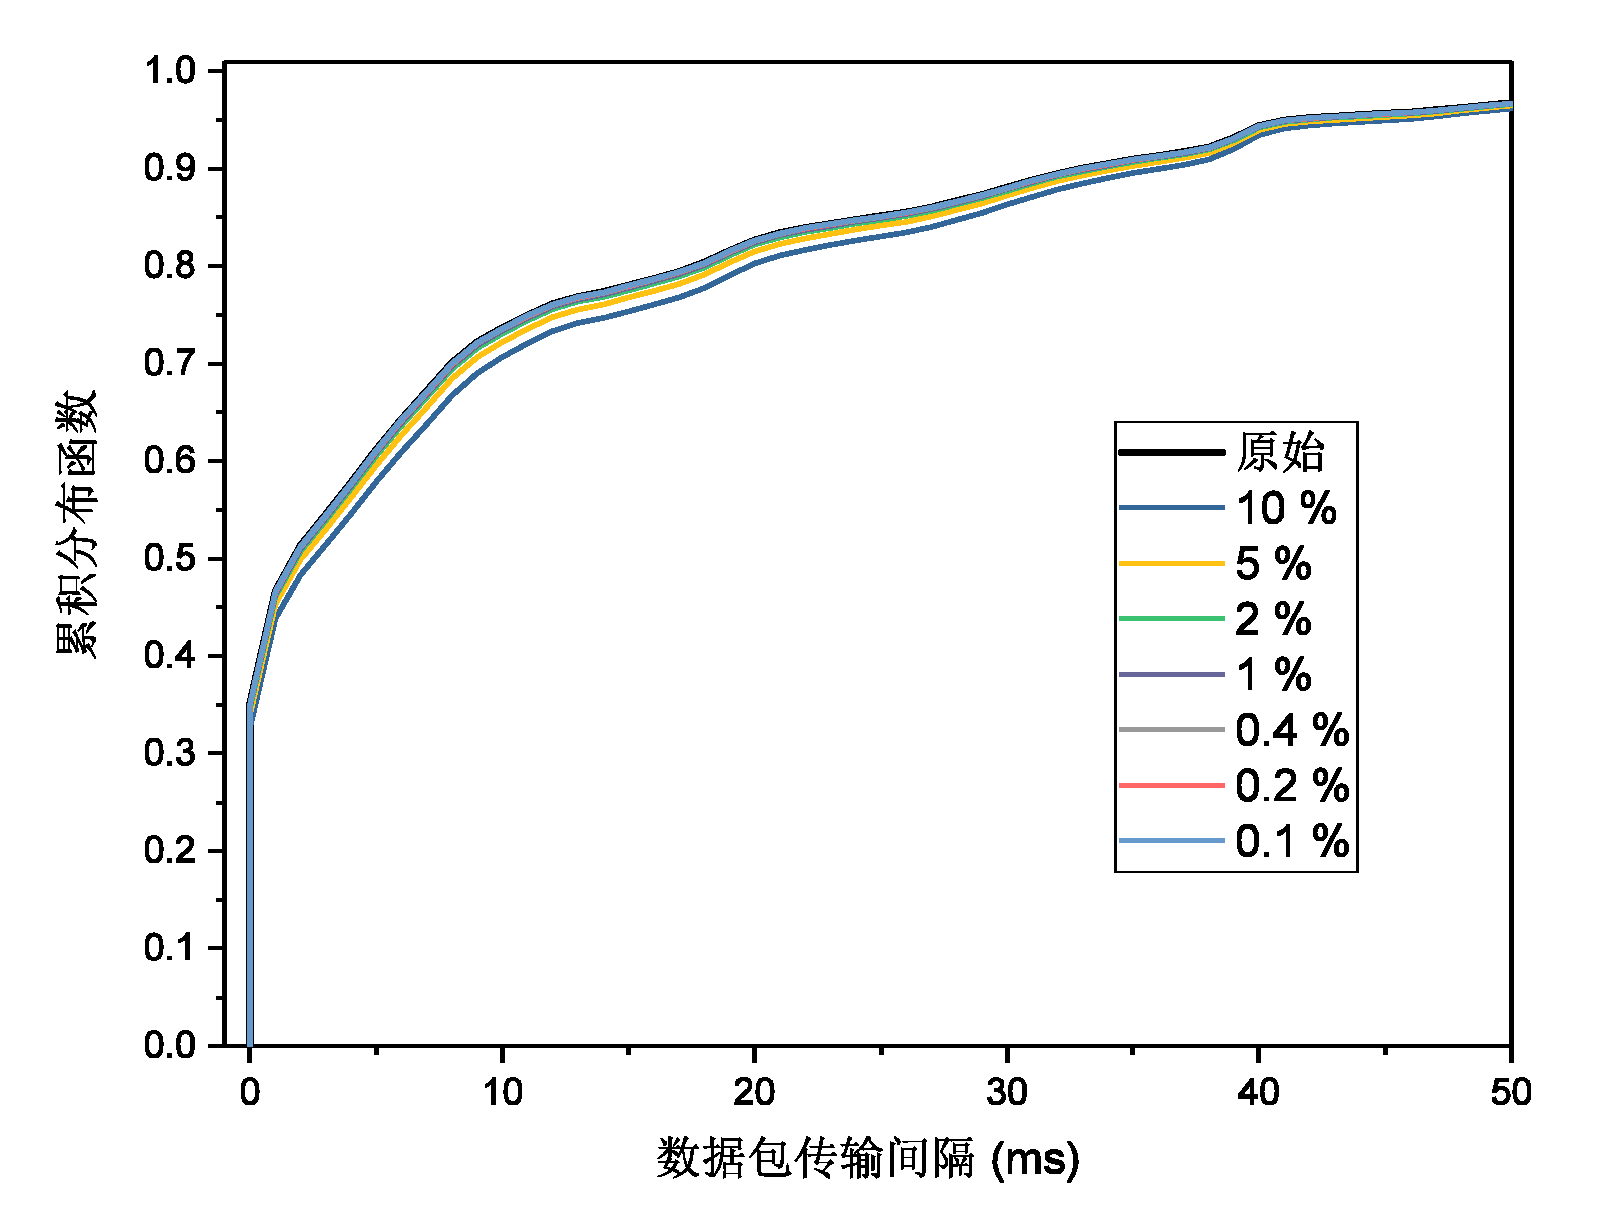
\includegraphics[width=0.48\textwidth]{chapters/chapter3/figures/ipd-cdf-excellent.pdf}
        }
        \subfigure[Good场景的CDF曲线]{
            \label{fig:3:result:ipd:cdf:good}
            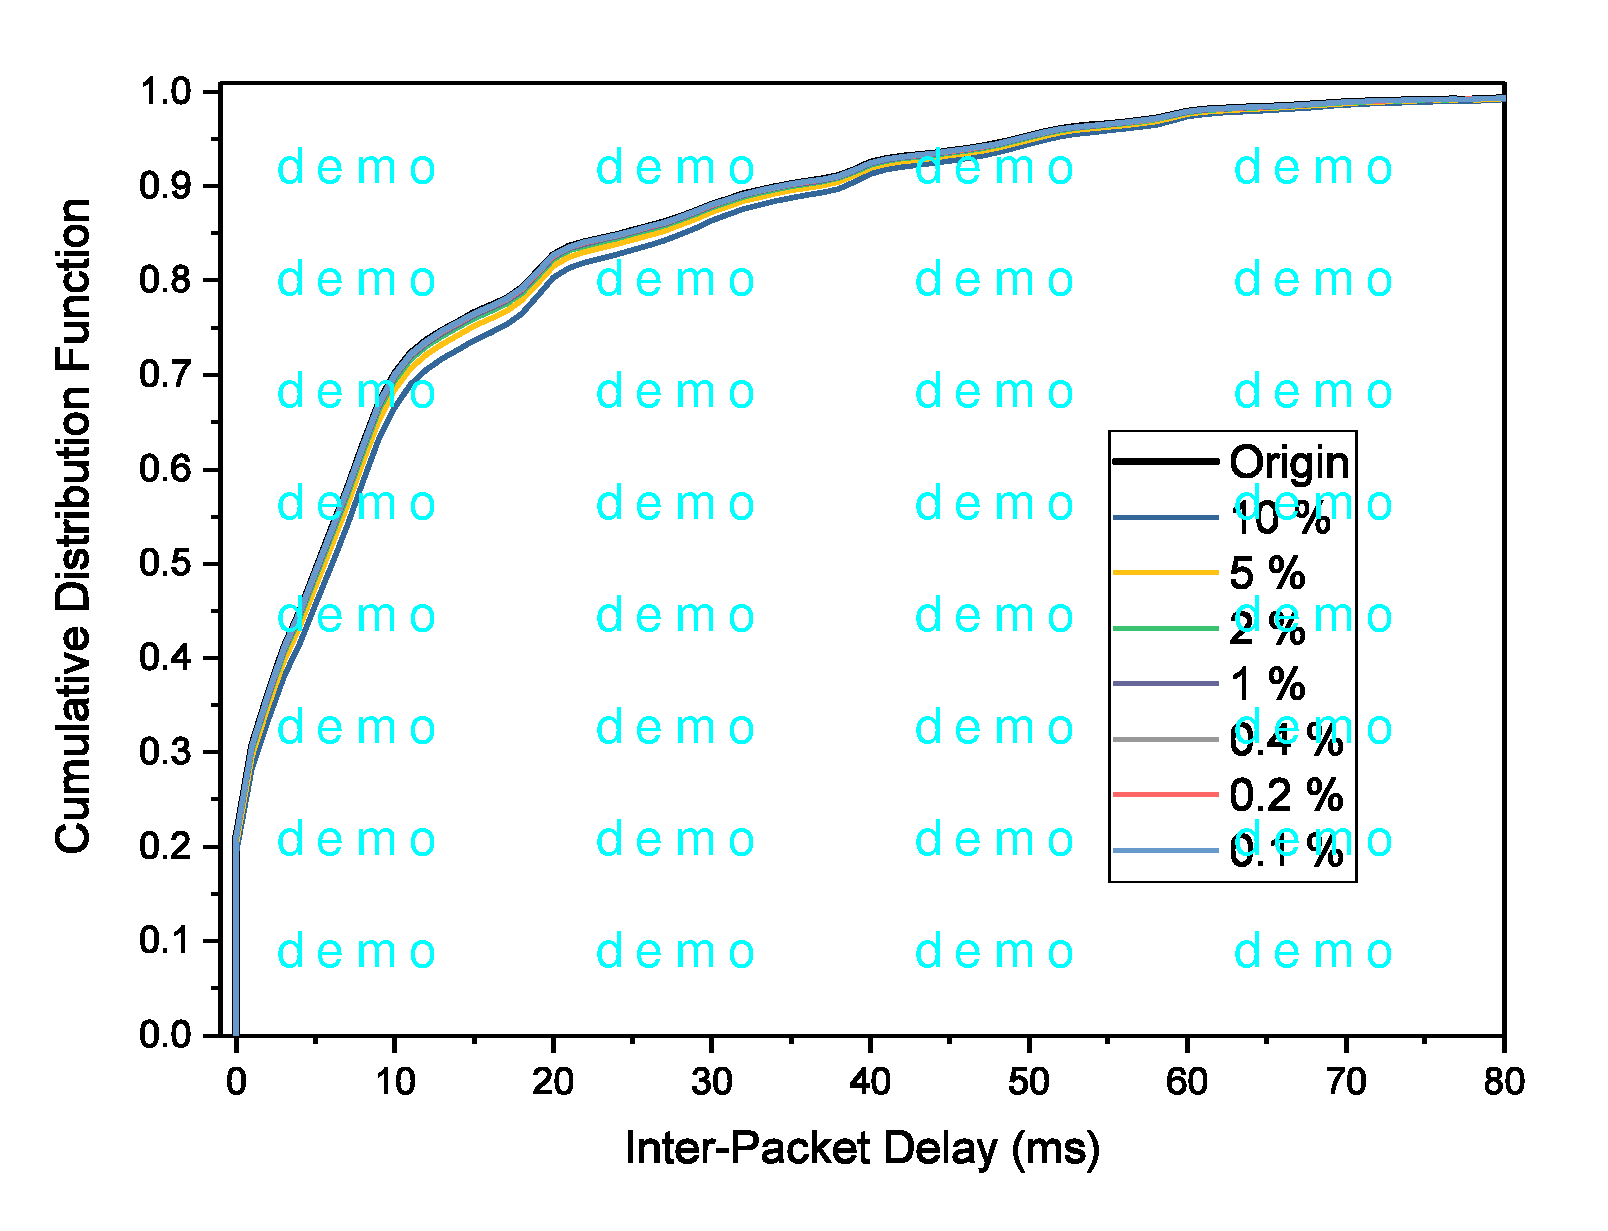
\includegraphics[width=0.48\textwidth]{chapters/chapter3/figures/ipd-cdf-good.pdf}
        }
        \caption{IPD分布的CDF曲线}
        \label{fig:3:result:ipd:cdf}
	\end{figure}
}

如图\ \nref{fig:3:result:ipd:cdf},虽然时间隐通道的分布与参照分布不完全重合,但总体趋势仍保持一致。即使主动丢包率上升到10\%,曲线仍未出现偏离。因此,时间隐通道的IPD分布可以通过CDF检测。

\subsubsection{条件熵检测结果}
\label{chap:analyze:result:ipd:kld}

\insertFigure{
    \begin{figure}[htb]
        \centering
        \subfigure[Excellent场景的箱线图]{
            \label{fig:3:result:ipd:kld:excellent}
            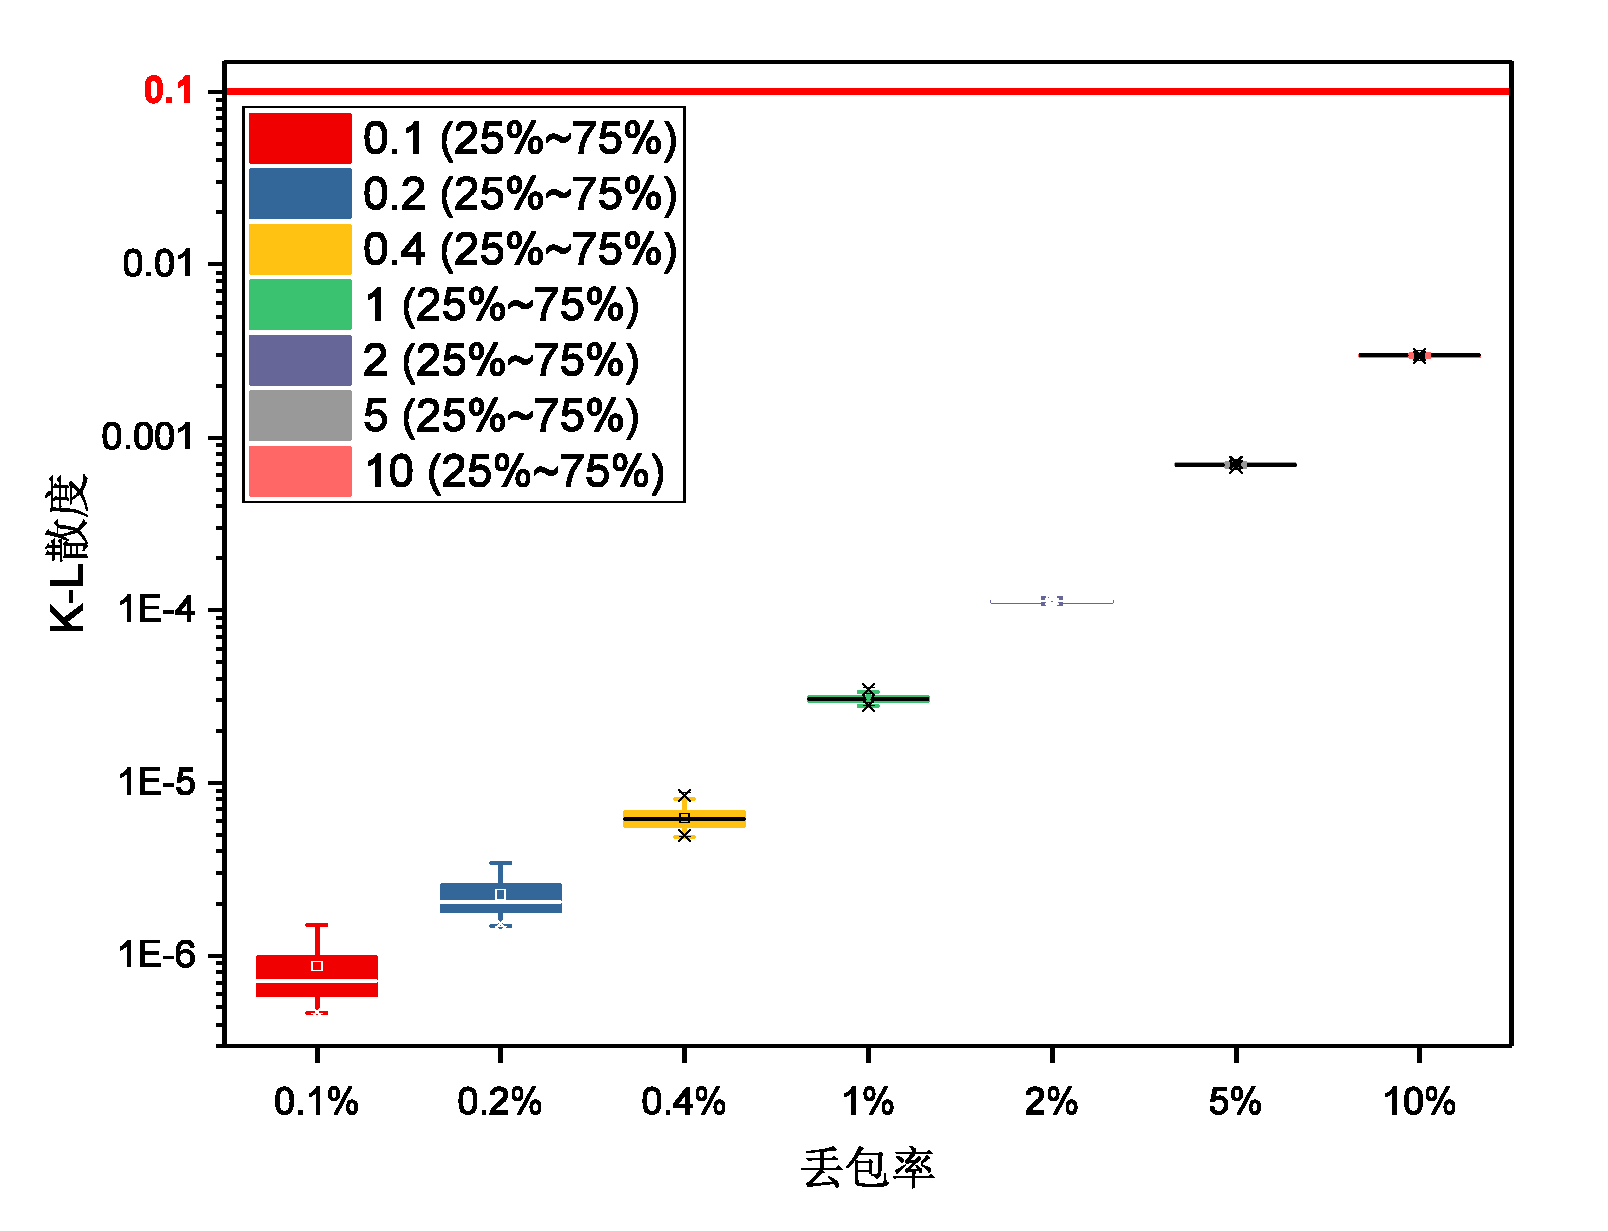
\includegraphics[width=0.48\textwidth]{chapters/chapter3/figures/ipd-kld-excellent.pdf}
        }
        \subfigure[Good场景的箱线图]{
            \label{fig:3:result:ipd:kld:good}
            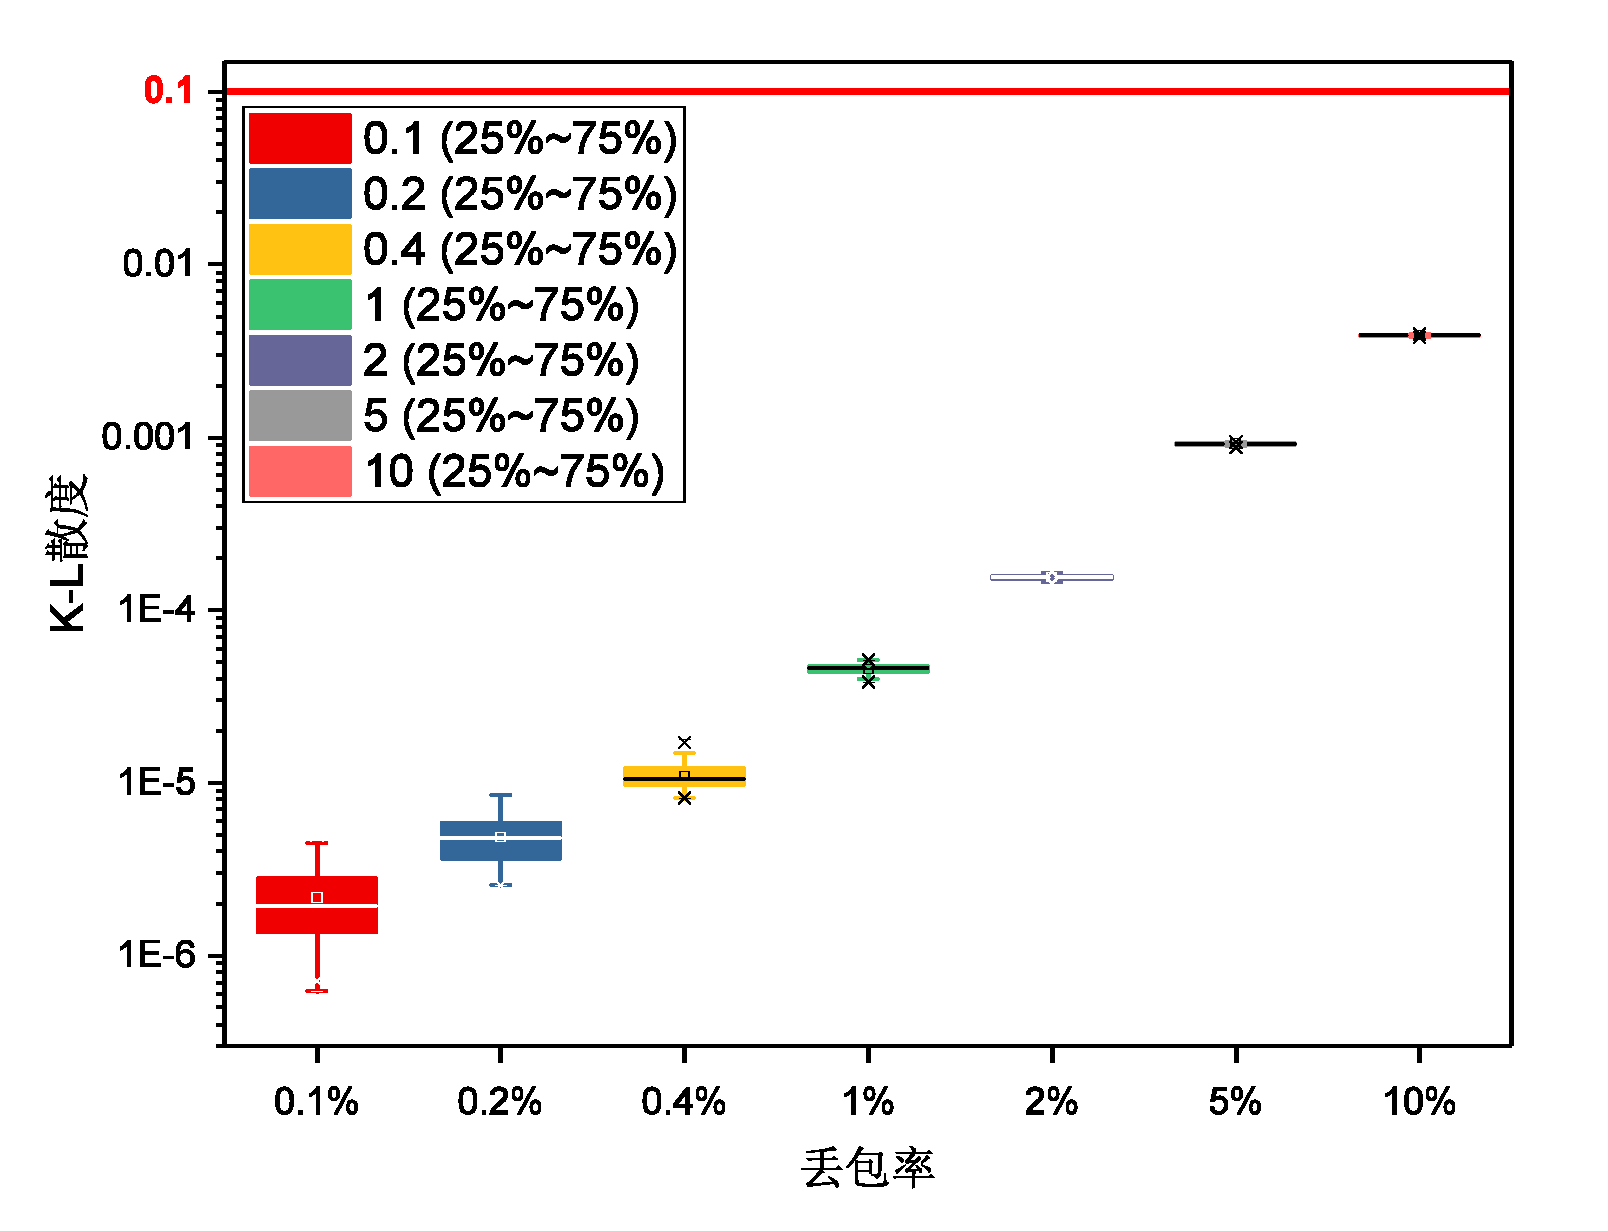
\includegraphics[width=0.48\textwidth]{chapters/chapter3/figures/ipd-kld-good.pdf}
        }
        \caption{IPD分布K-L散度检测结果的箱线图}
        \label{fig:3:result:ipd:kld}
	\end{figure}
}

如图\ \nref{fig:3:result:ipd:kld},两种场景中对IPD分布的条件熵检测结果汇总为箱线图。两种场景中,K-L散度检测结果均小于阈值0.1。随着主动丢包率的降低,K-L散度逐渐下降,意味着隐通道的IPD分布与宿主信道的IPD分布更加接近。

\subsubsection{一致性检验检测结果}
\label{chap:analyze:result:ipd:statistical}

\insertFigure{
    \begin{figure}[htb]
        \centering
        \subfigure[Excellent场景p值的箱线图]{
            \label{fig:3:result:ipd:ks:excellent}
            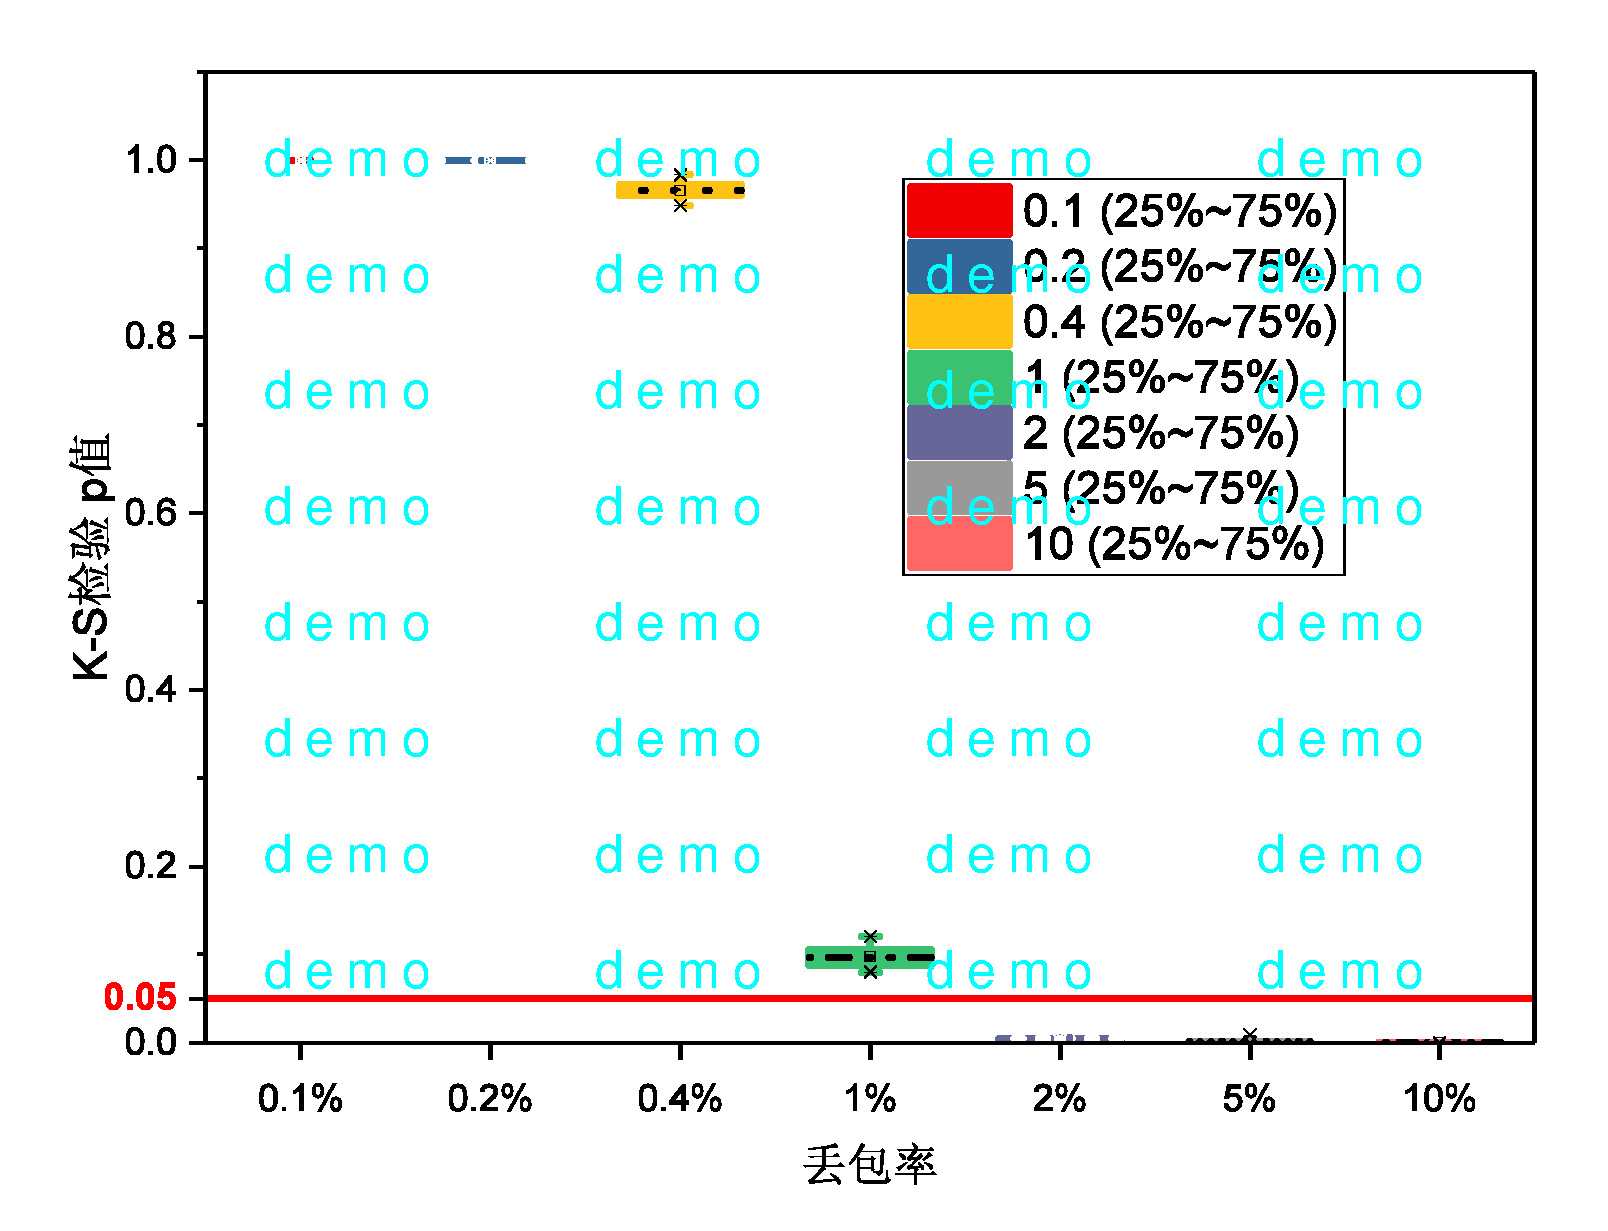
\includegraphics[width=0.48\textwidth]{chapters/chapter3/figures/ipd-ks-excellent.pdf}
        }
        \subfigure[Good场景p值的箱线图]{
            \label{fig:3:result:ipd:ks:good}
            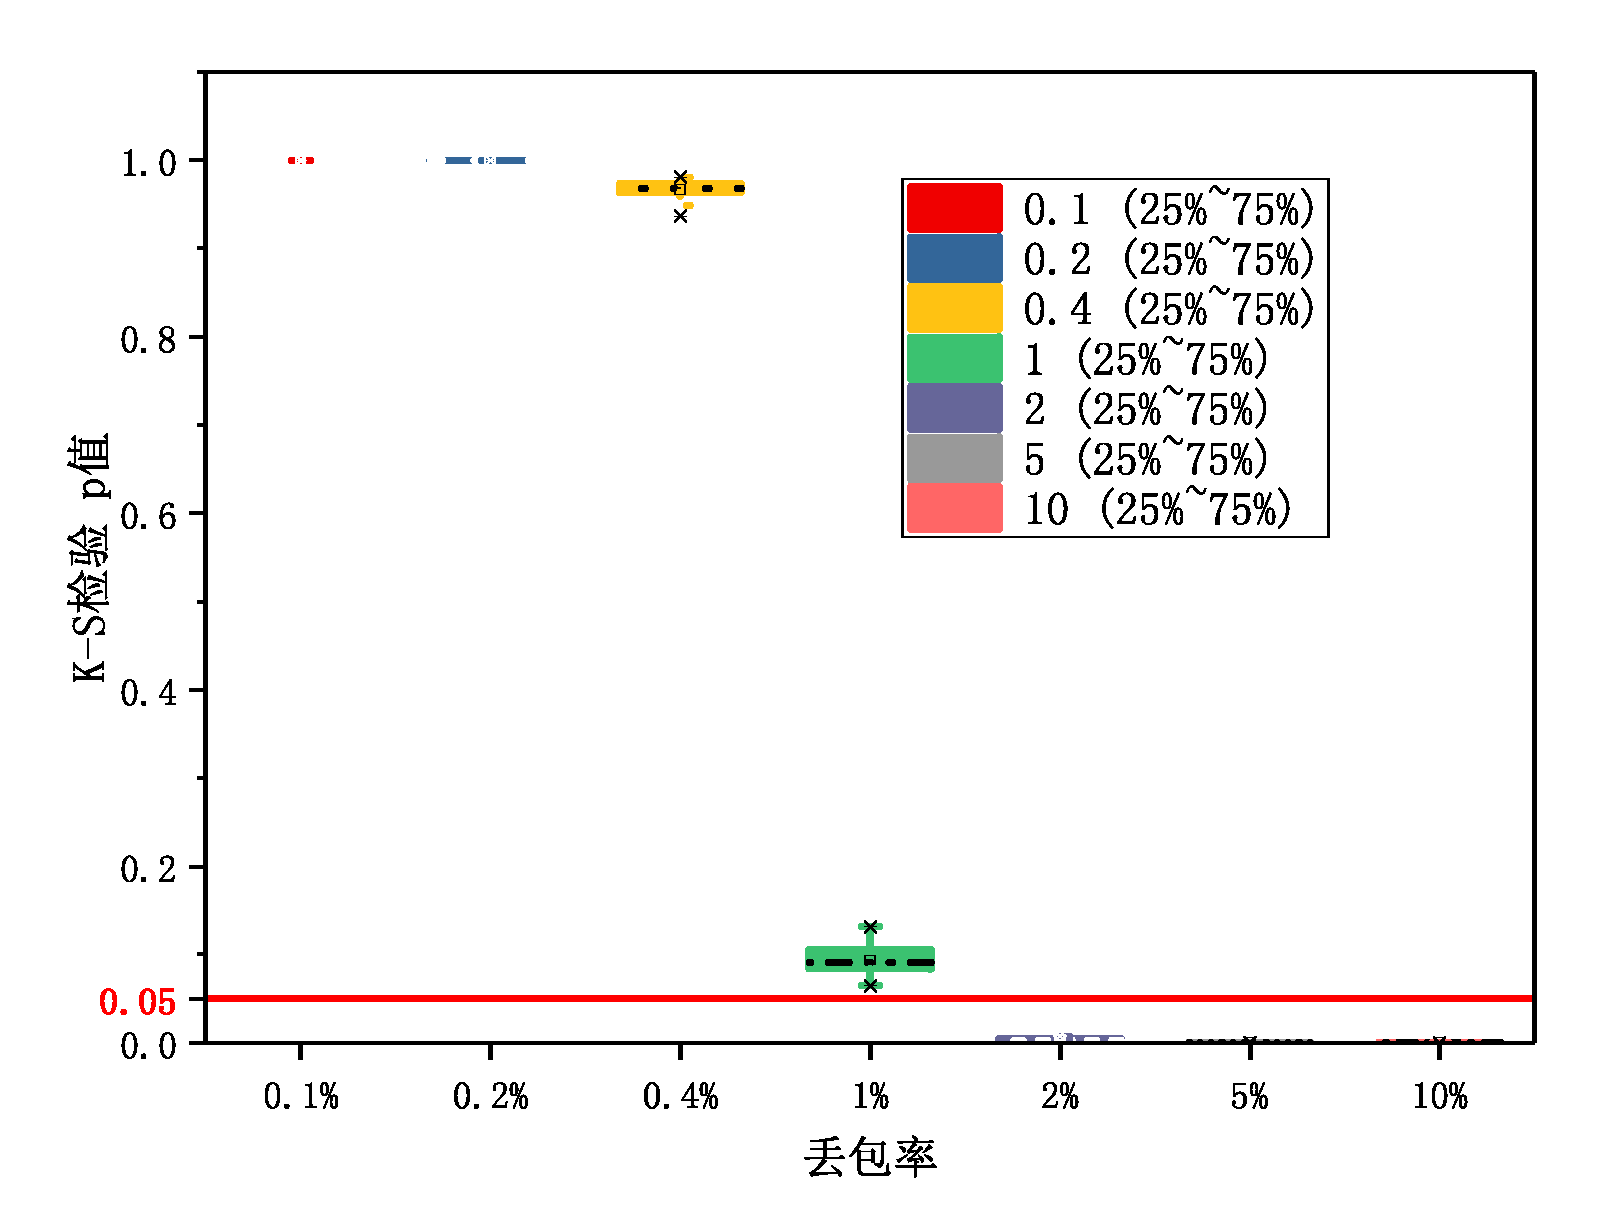
\includegraphics[width=0.48\textwidth]{chapters/chapter3/figures/ipd-ks-good.pdf}
        }
        \caption{IPD分布K-S检验结果的箱线图}
        \label{fig:3:result:ipd:ks}
	\end{figure}

	\begin{figure}[htb]
        \centering
        \subfigure[Excellent场景p值的箱线图]{
            \label{fig:3:result:ipd:t:excellent}
            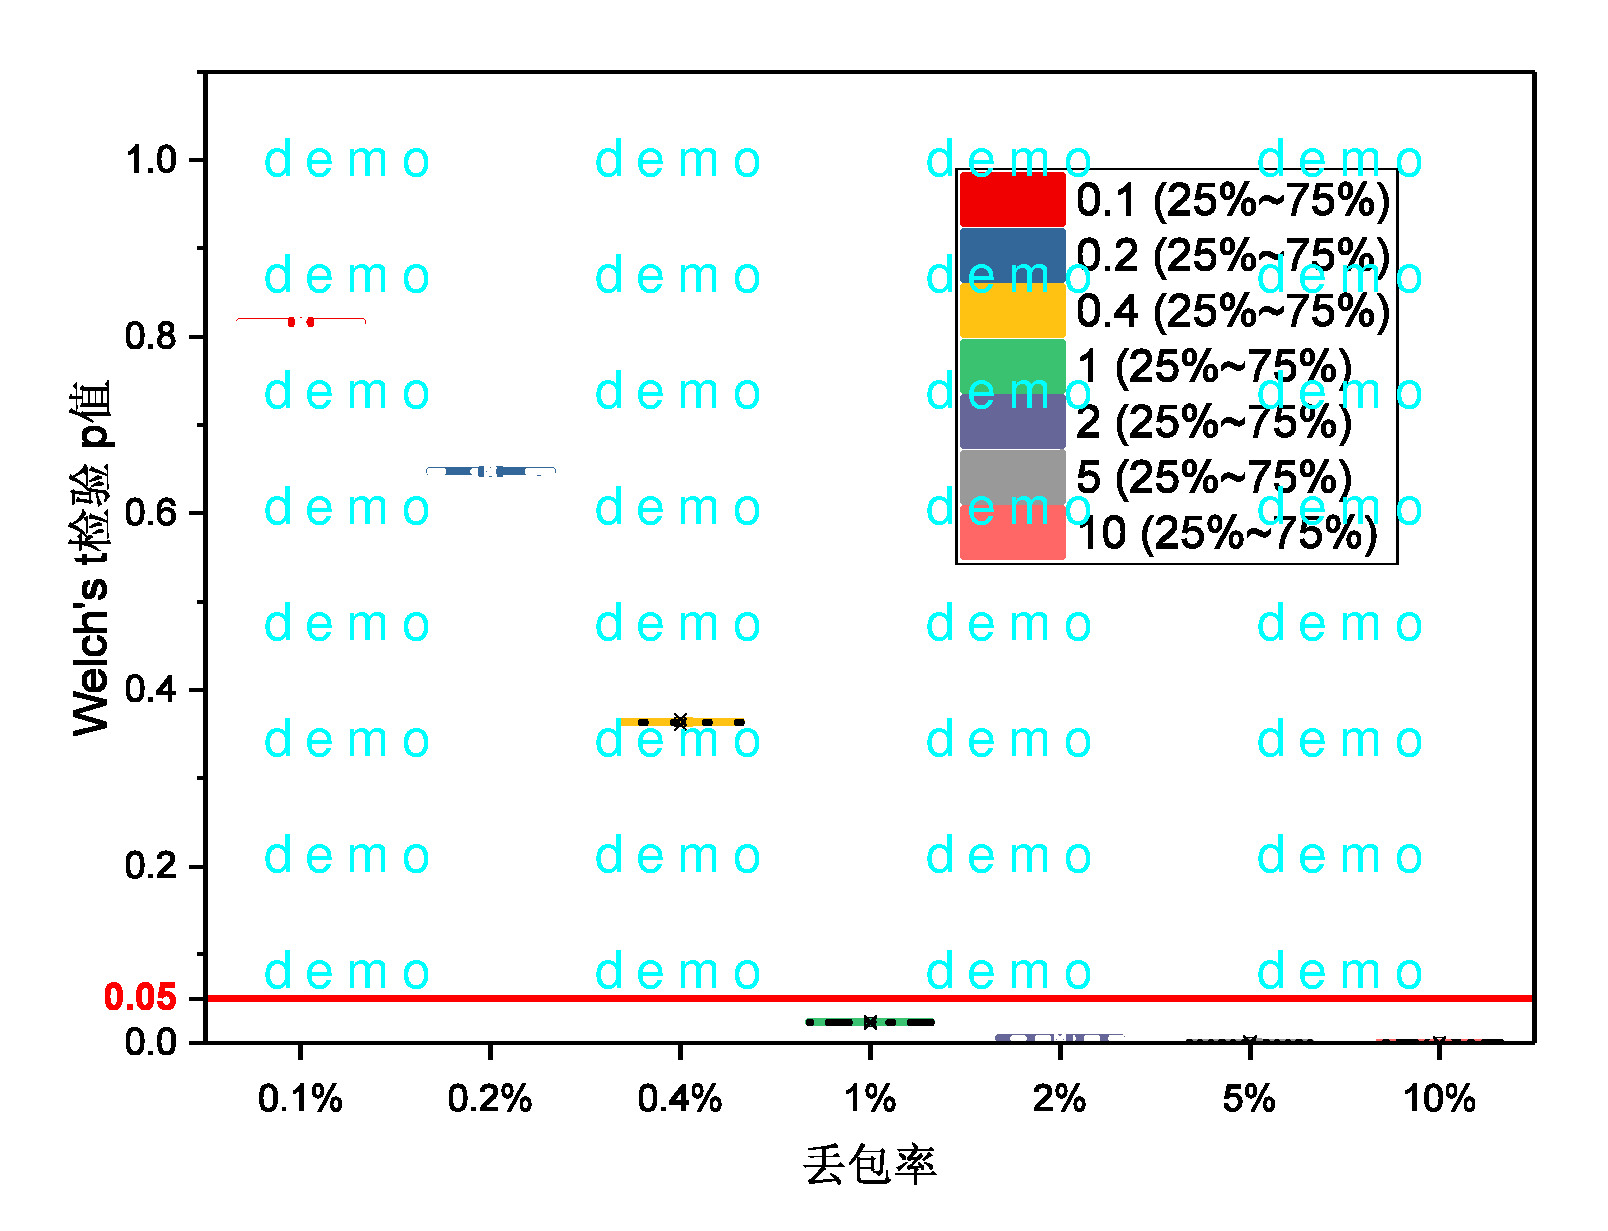
\includegraphics[width=0.48\textwidth]{chapters/chapter3/figures/ipd-t-excellent.pdf}
        }
        \subfigure[Good场景p值的箱线图]{
            \label{fig:3:result:ipd:t:good}
            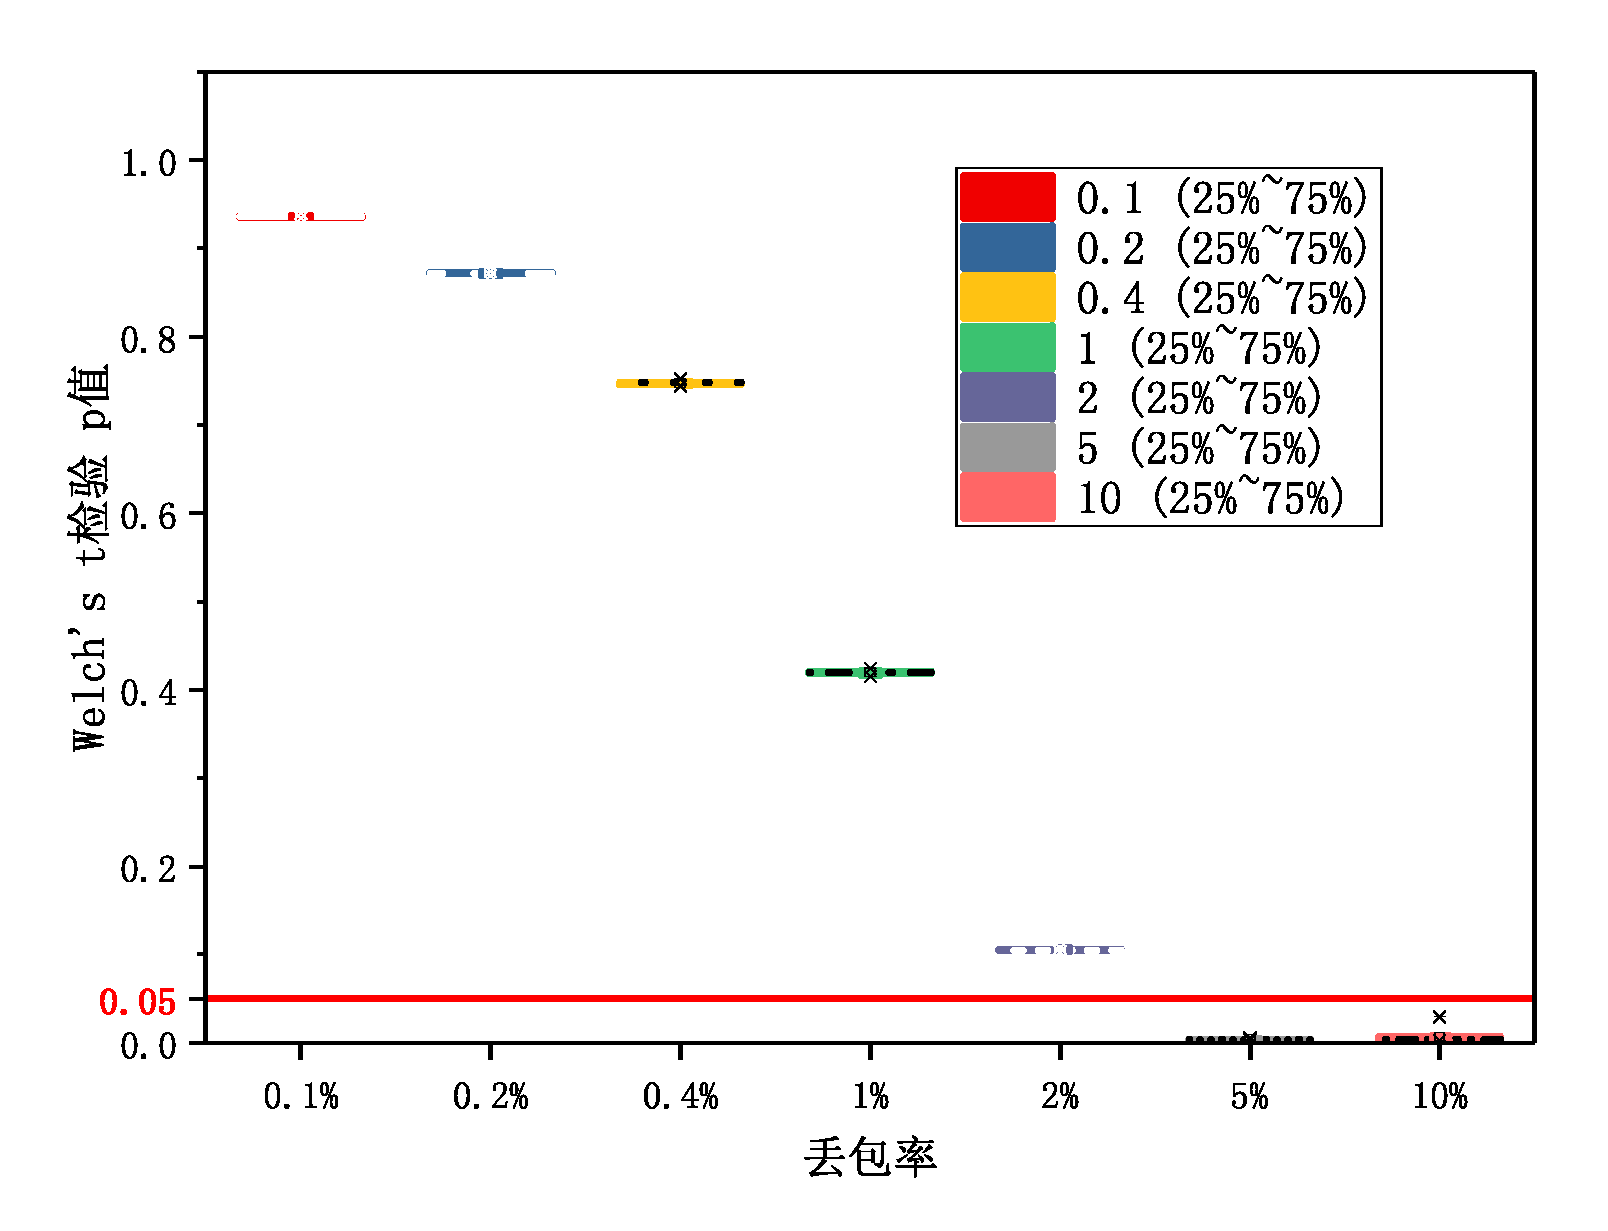
\includegraphics[width=0.48\textwidth]{chapters/chapter3/figures/ipd-t-good.pdf}
        }
        \caption{IPD分布Welch's t检验结果的箱线图}
        \label{fig:3:result:ipd:t}
	\end{figure}

	\begin{figure}[htb]
        \centering
        \subfigure[Excellent场景p值的箱线图]{
            \label{fig:3:result:ipd:mw:excellent}
            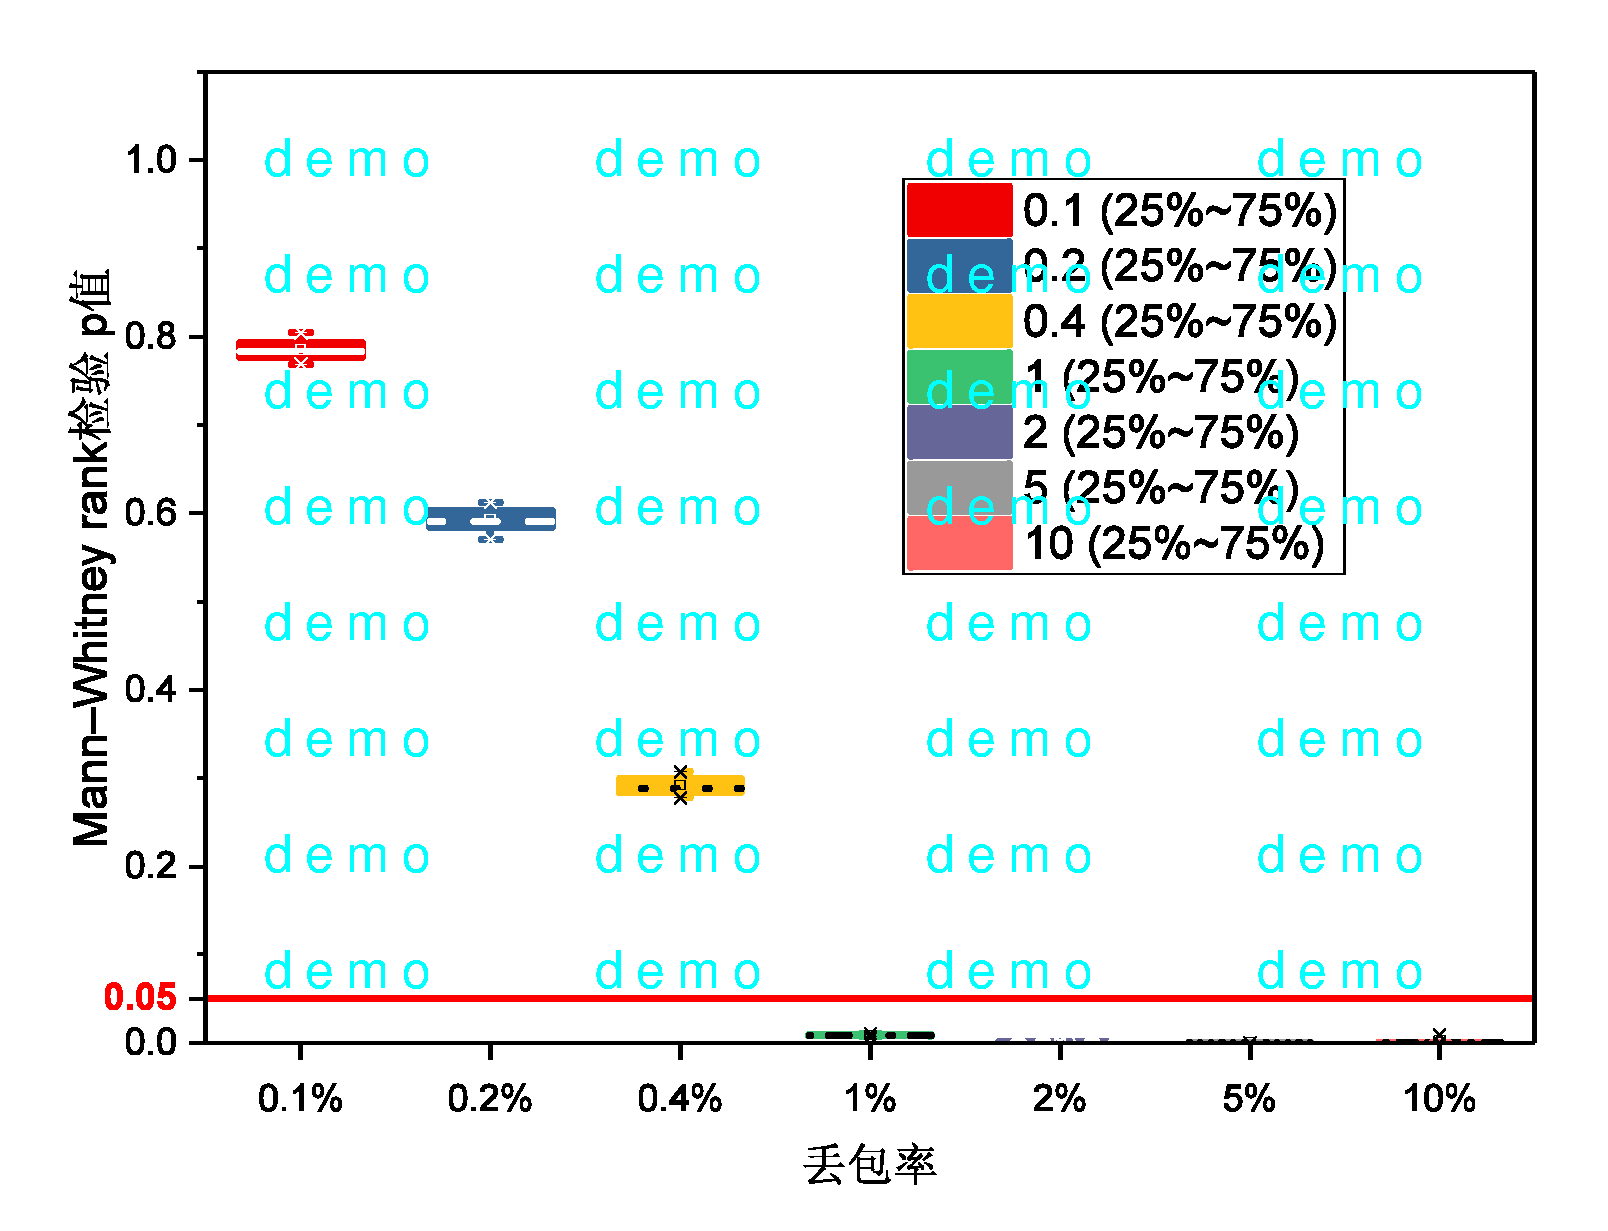
\includegraphics[width=0.48\textwidth]{chapters/chapter3/figures/ipd-mw-excellent.pdf}
        }
        \subfigure[Good场景p值的箱线图]{
            \label{fig:3:result:ipd:mw:good}
            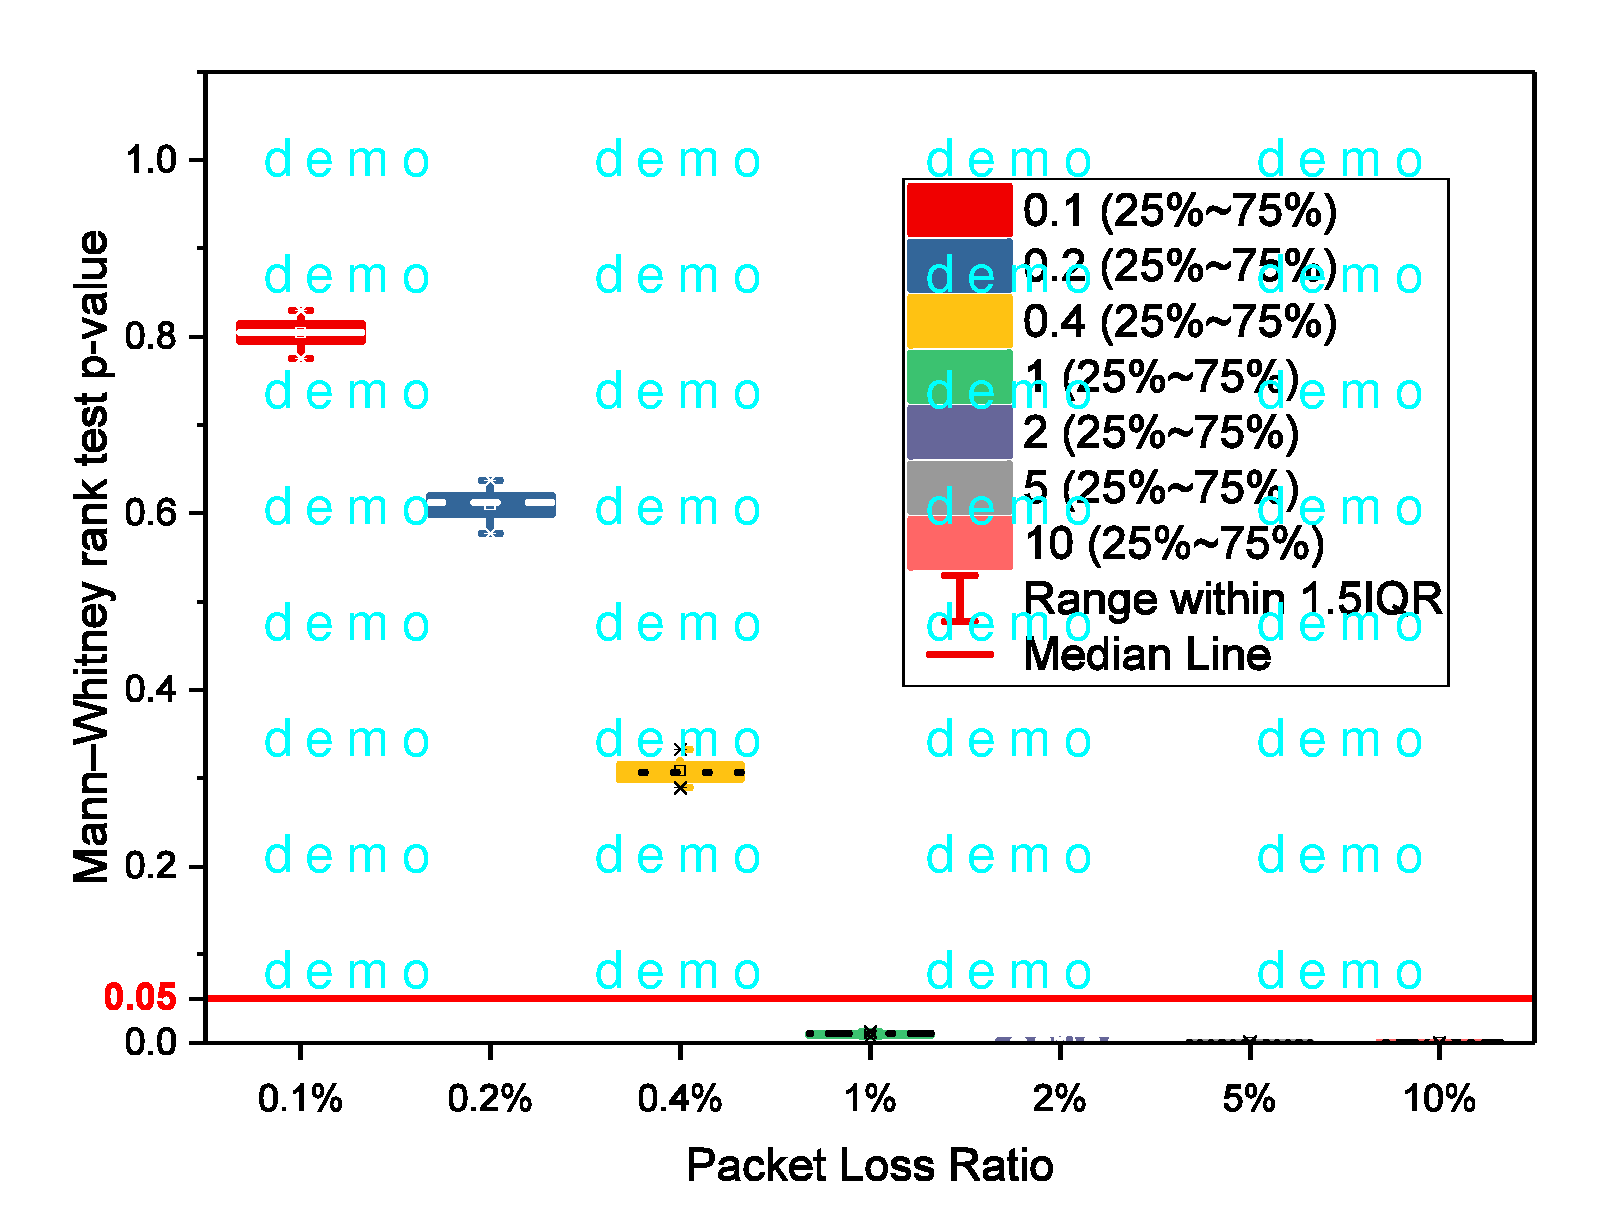
\includegraphics[width=0.48\textwidth]{chapters/chapter3/figures/ipd-mw-good.pdf}
        }
        \caption{IPD分布Mann–Whitney rank检验结果的箱线图}
        \label{fig:3:result:ipd:mw}
	\end{figure}
}

如图\ \nref{fig:3:result:ipd:ks},通过K-S检验,已经检测出部分时间隐通道。当主动丢包率$\le 1\%$时,IPD分布通过了K-S检验,并且随着主动丢包率的进一步降低,K-S检验的p值逐渐增大。如图\ \nref{fig:3:result:ipd:t},Welch's t检验中,已经检测出大部分时间隐通道。Excellent场景中,当主动丢包率$\le 0.4\%$后,才通过Welch's t检验;而Good场景中,当主动丢包率$\le 2\%$时,即可通过Welch's t检验。Welch's t检验结果表明,不同的场景中,丢包导致的IPD平均值变化程度不同。

如图\ \nref{fig:3:result:ipd:mw},Mann–Whitney rank检验中,只有主动丢包率$\le 0.4\%$才通过检测。由于Mann–Whitney rank检验适用的样本分布为均匀分布,所以检验结果较Welch's t检验更加严格。

\subsubsection{相对距离检测结果}
\label{chap:analyze:result:ipd:distance}

\insertFigure{
	\begin{figure}[htb]
        \centering
        \subfigure[Excellent场景Wasserstein距离的箱线图]{
            \label{fig:3:result:ipd:wd:excellent}
            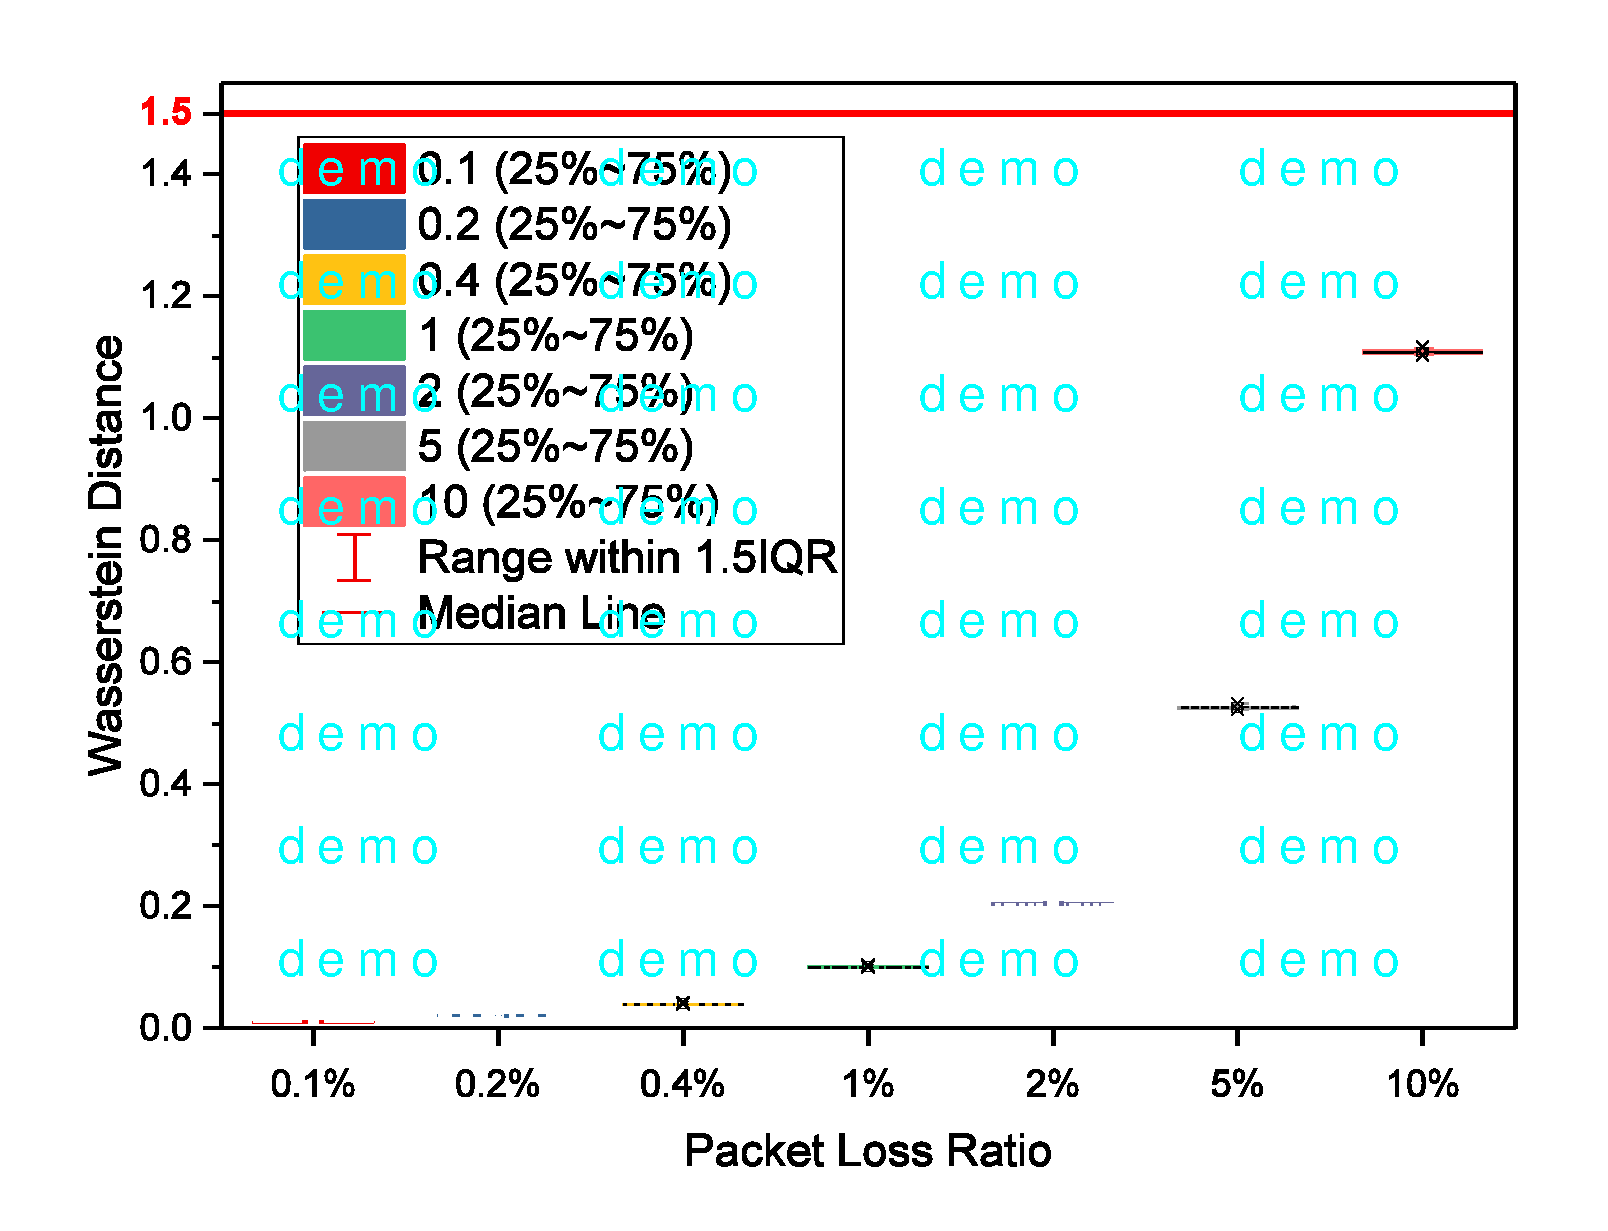
\includegraphics[width=0.48\textwidth]{chapters/chapter3/figures/ipd-wd-excellent.pdf}
        }
        \subfigure[Good场景Wasserstein距离的箱线图]{
            \label{fig:3:result:ipd:wd:good}
            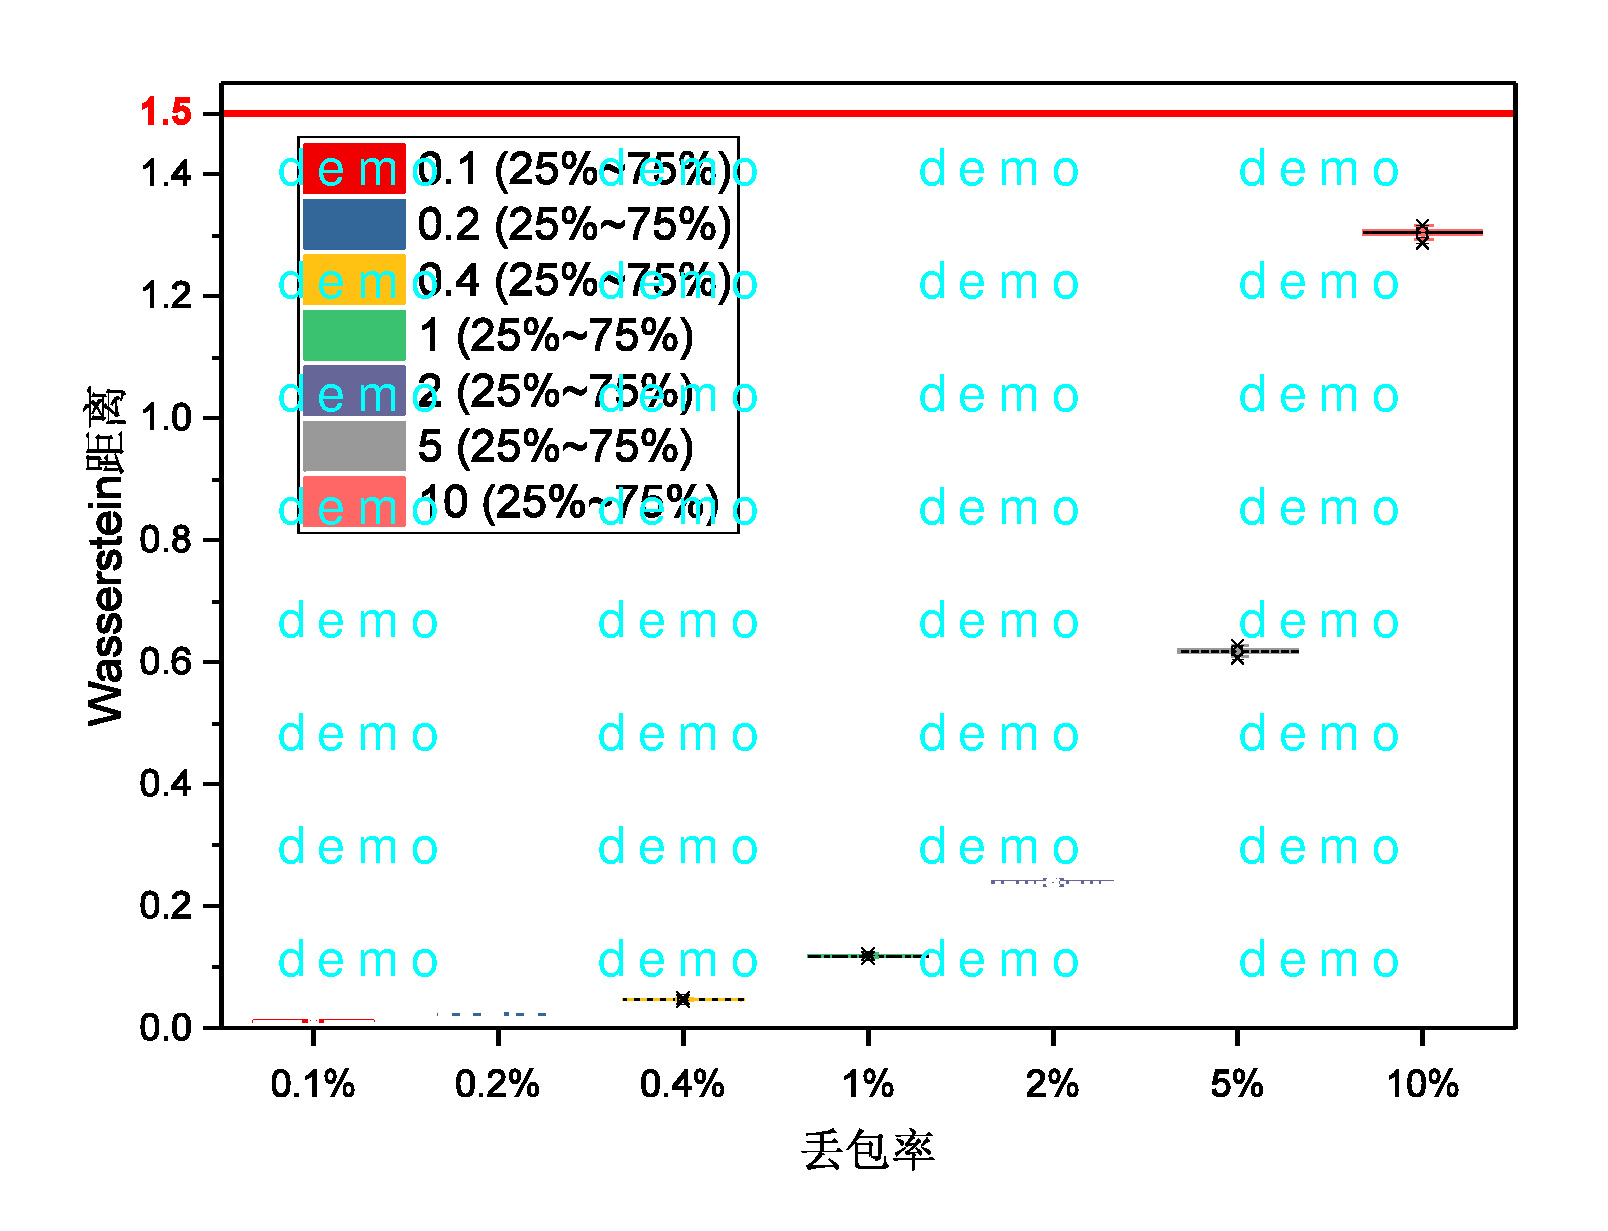
\includegraphics[width=0.48\textwidth]{chapters/chapter3/figures/ipd-wd-good.pdf}
        }
        \caption{IPD分布Wasserstein距离检测的箱线图}
        \label{fig:3:result:ipd:wd}
	\end{figure}

	\begin{figure}[htb]
        \centering
        \subfigure[Excellent场景能量距离的箱线图]{
            \label{fig:3:result:ipd:ed:excellent}
            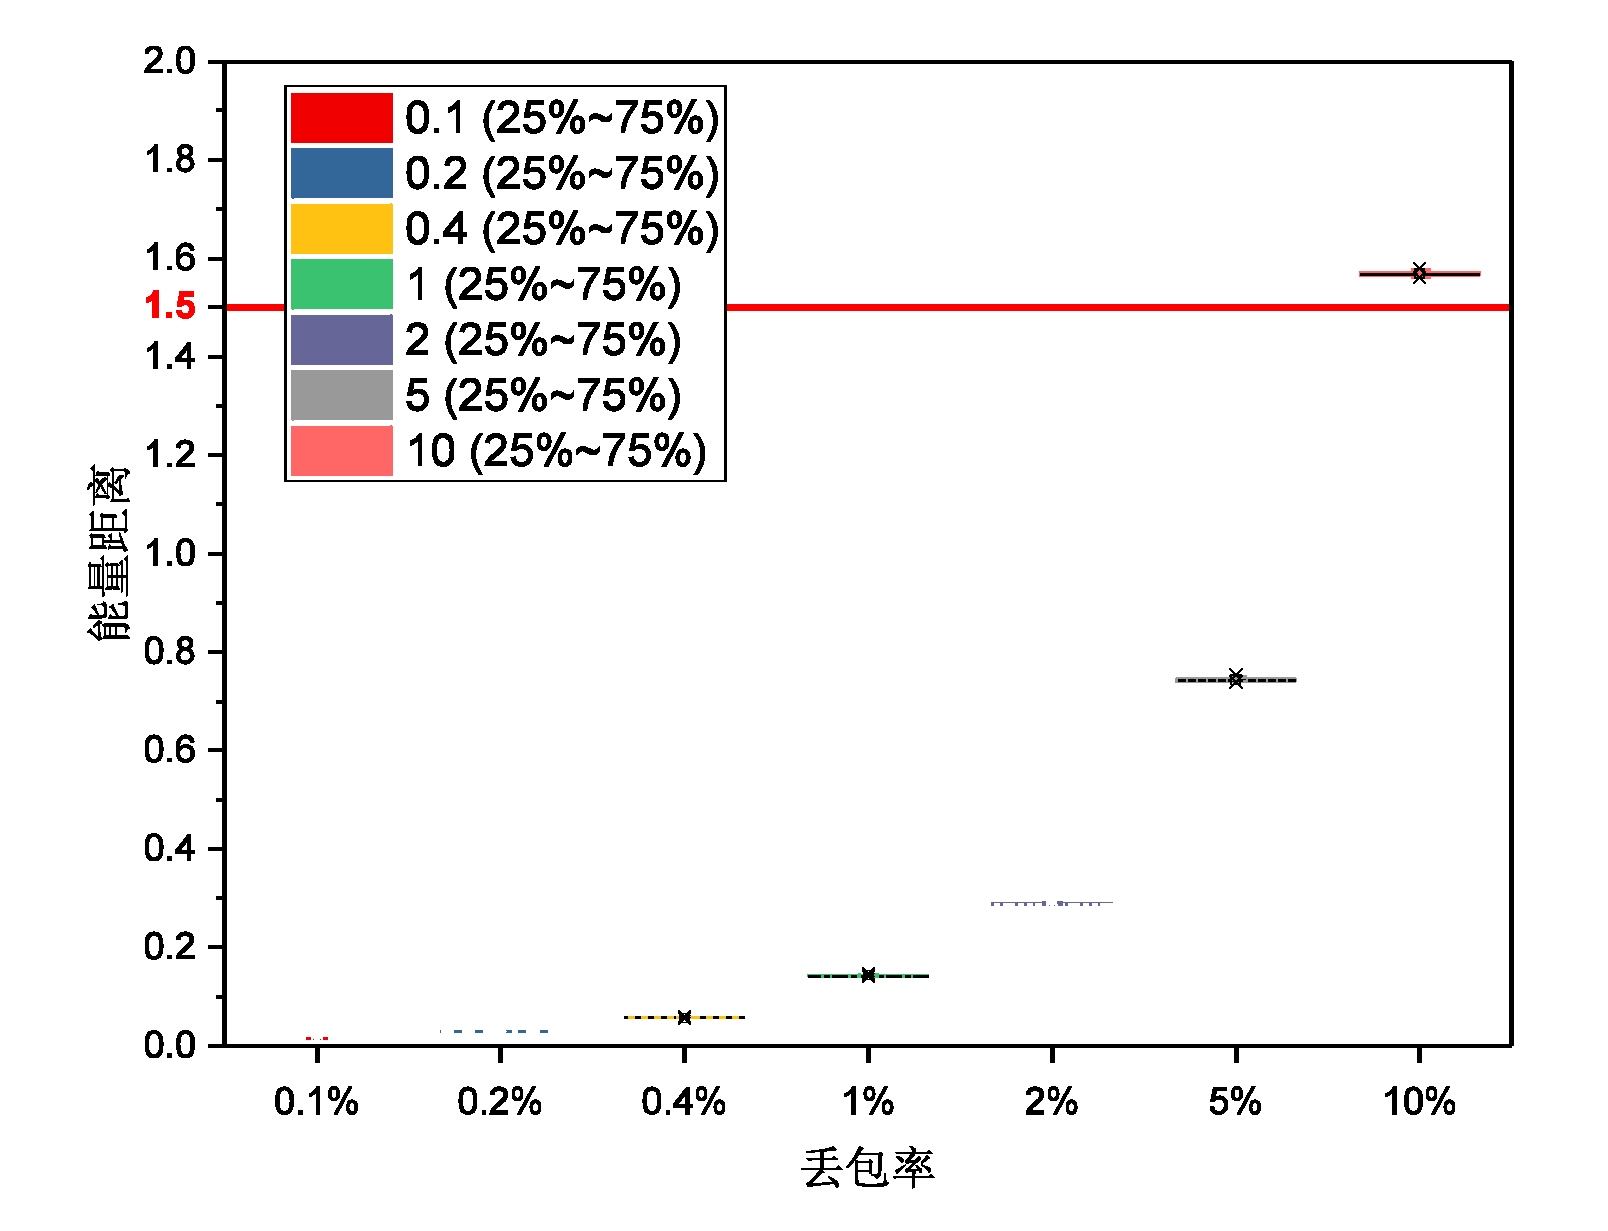
\includegraphics[width=0.48\textwidth]{chapters/chapter3/figures/ipd-ed-excellent.pdf}
        }
        \subfigure[Good场景能量距离的箱线图]{
            \label{fig:3:result:ipd:ed:good}
            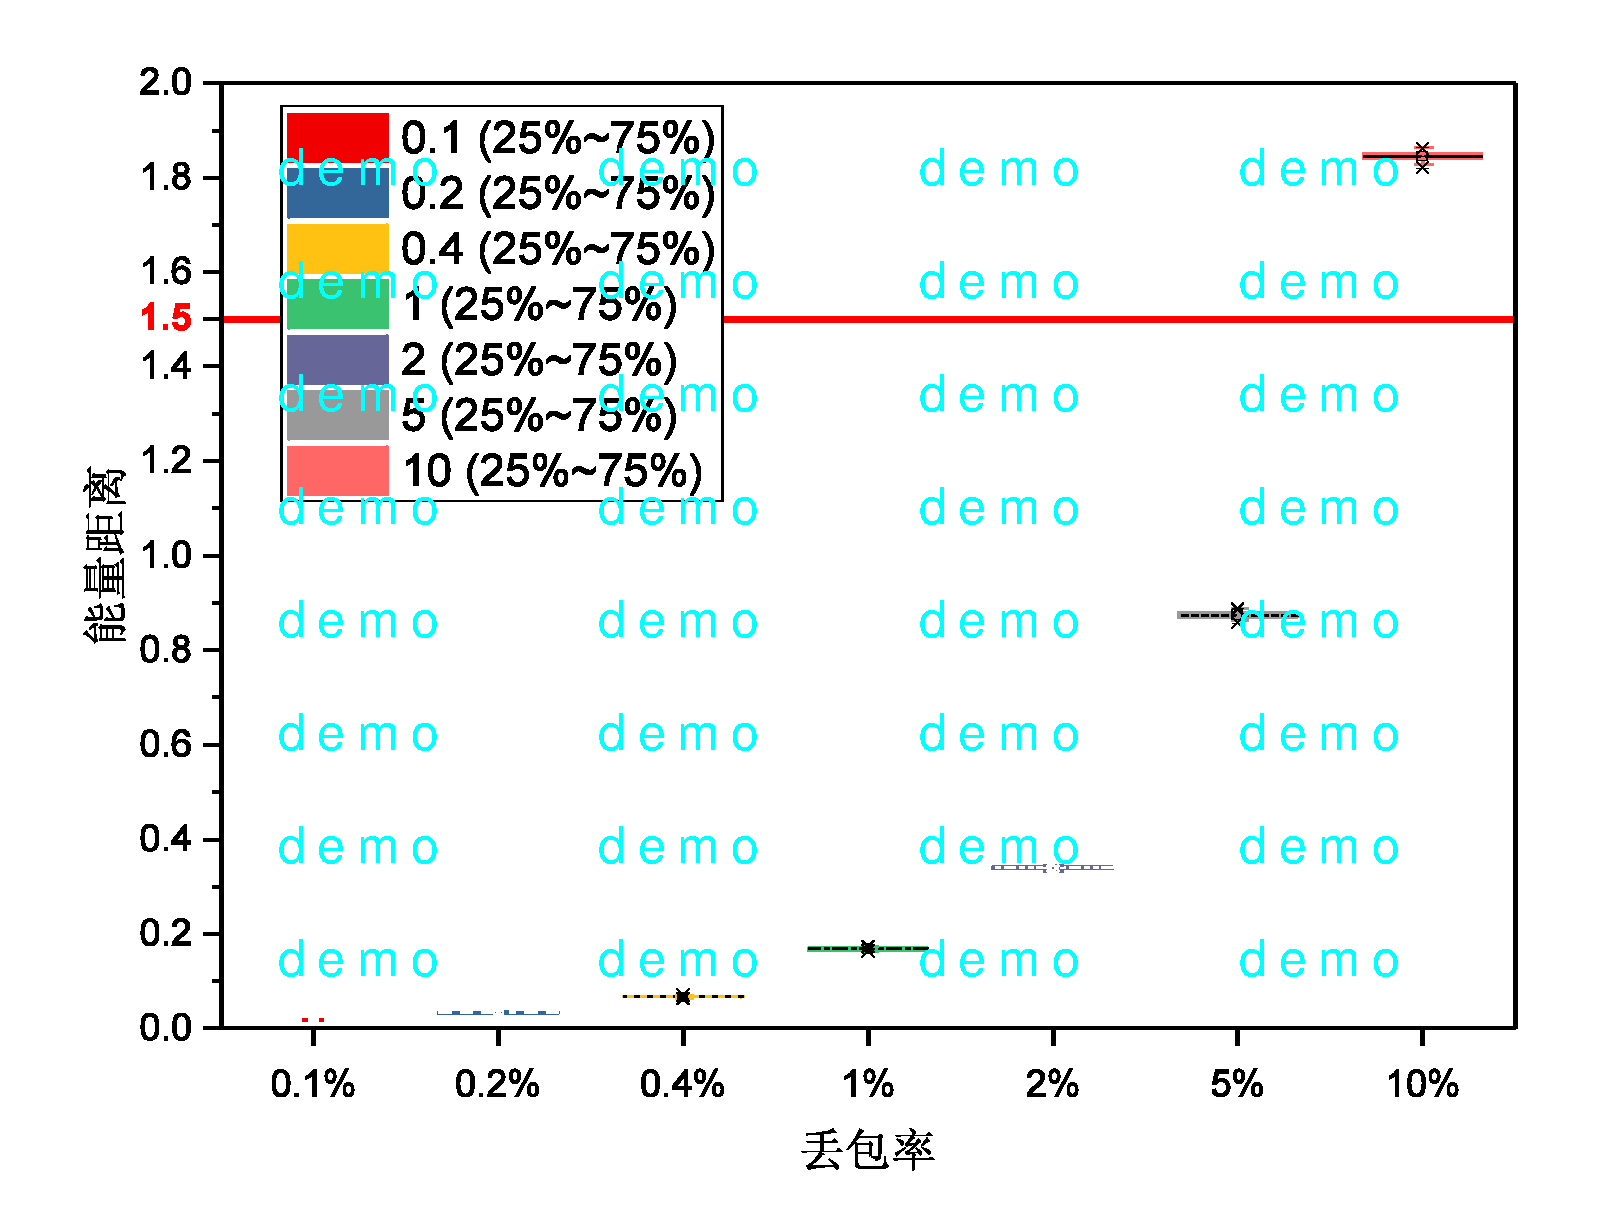
\includegraphics[width=0.48\textwidth]{chapters/chapter3/figures/ipd-ed-good.pdf}
        }
        \caption{IPD分布能量距离检测的箱线图}
        \label{fig:3:result:ipd:ed}
	\end{figure}
}

如图\ \nref{fig:3:result:ipd:wd},主动丢包率与Wasserstein距离呈正相关。两种场景中检测结果相同,虽然当主动丢包率为$10\%$时已经接近阈值,但仍未超过阈值,因此无法断定为时间隐通道。如图\ \nref{fig:3:result:ipd:ed},能量距离与主动丢包率也呈正相关。两种场景中,当主动丢包率$\le 5\%$时,才可通过检测。根据检测结果,能量距离较Wasserstein距离具有更高的要求,但二者具有一致的变化趋势。

根据以上测试结果,通过IPD分布检测基于主动丢包的时间隐通道,在灵敏度方面无法达到检测要求。其主要因素,在于丢包事件数量与IPD数量相比较少,少量的丢包不会导致IPD分布出现较大变动。因此,现有基于IPD的检测方法,无法有效检测基于主动丢包的时间隐通道。另一方面,实验结果表明,在当前的检测方法面前,基于主动丢包的时间隐通道具有较好的隐蔽性。

\subsection{连续丢包数检测结果评估}
\label{chap:analyze:result:burst}

\subsubsection{CDF检测结果}
\label{chap:analyze:result:burst:cdf}

\insertFigure{
    \begin{figure}[htb]
        \centering
        \subfigure[Excellent场景的CDF曲线]{
            \label{fig:3:result:burst:cdf:excellent}
            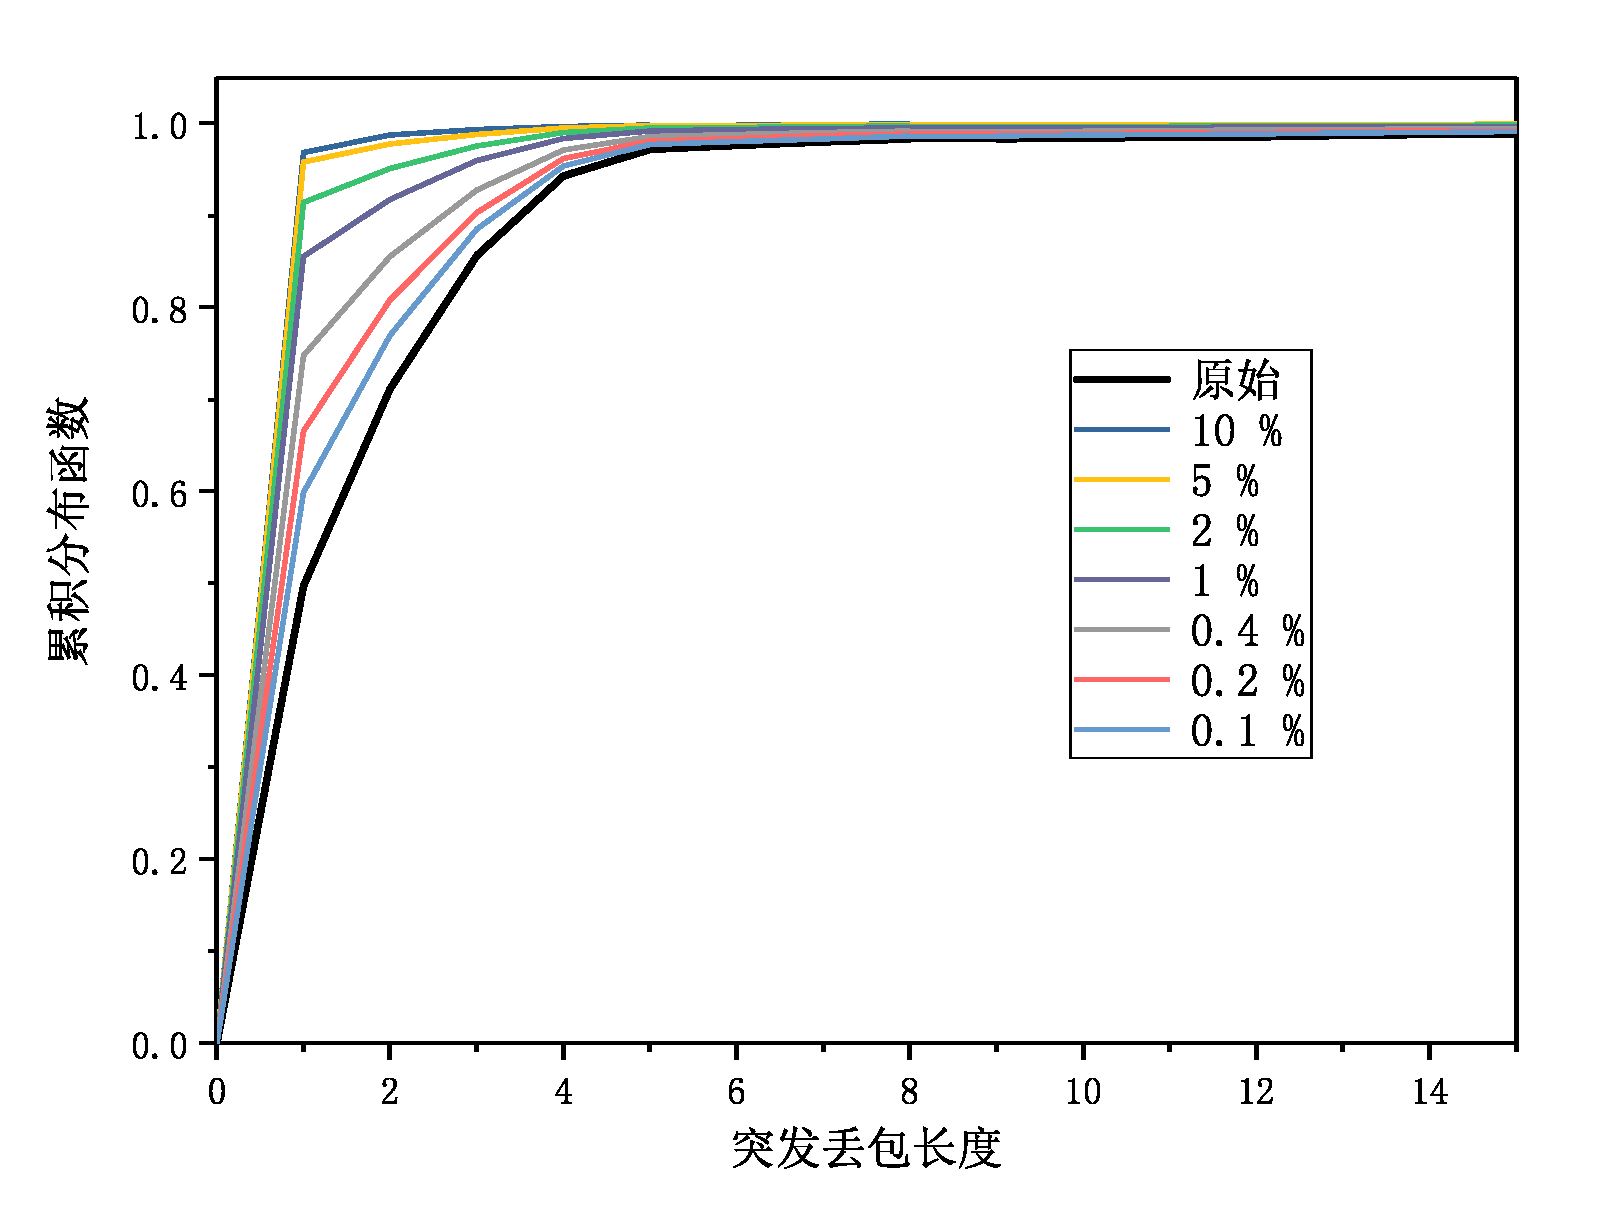
\includegraphics[width=0.48\textwidth]{chapters/chapter3/figures/burst-cdf-excellent.pdf}
        }
        \subfigure[Good场景的CDF曲线]{
            \label{fig:3:result:burst:cdf:good}
            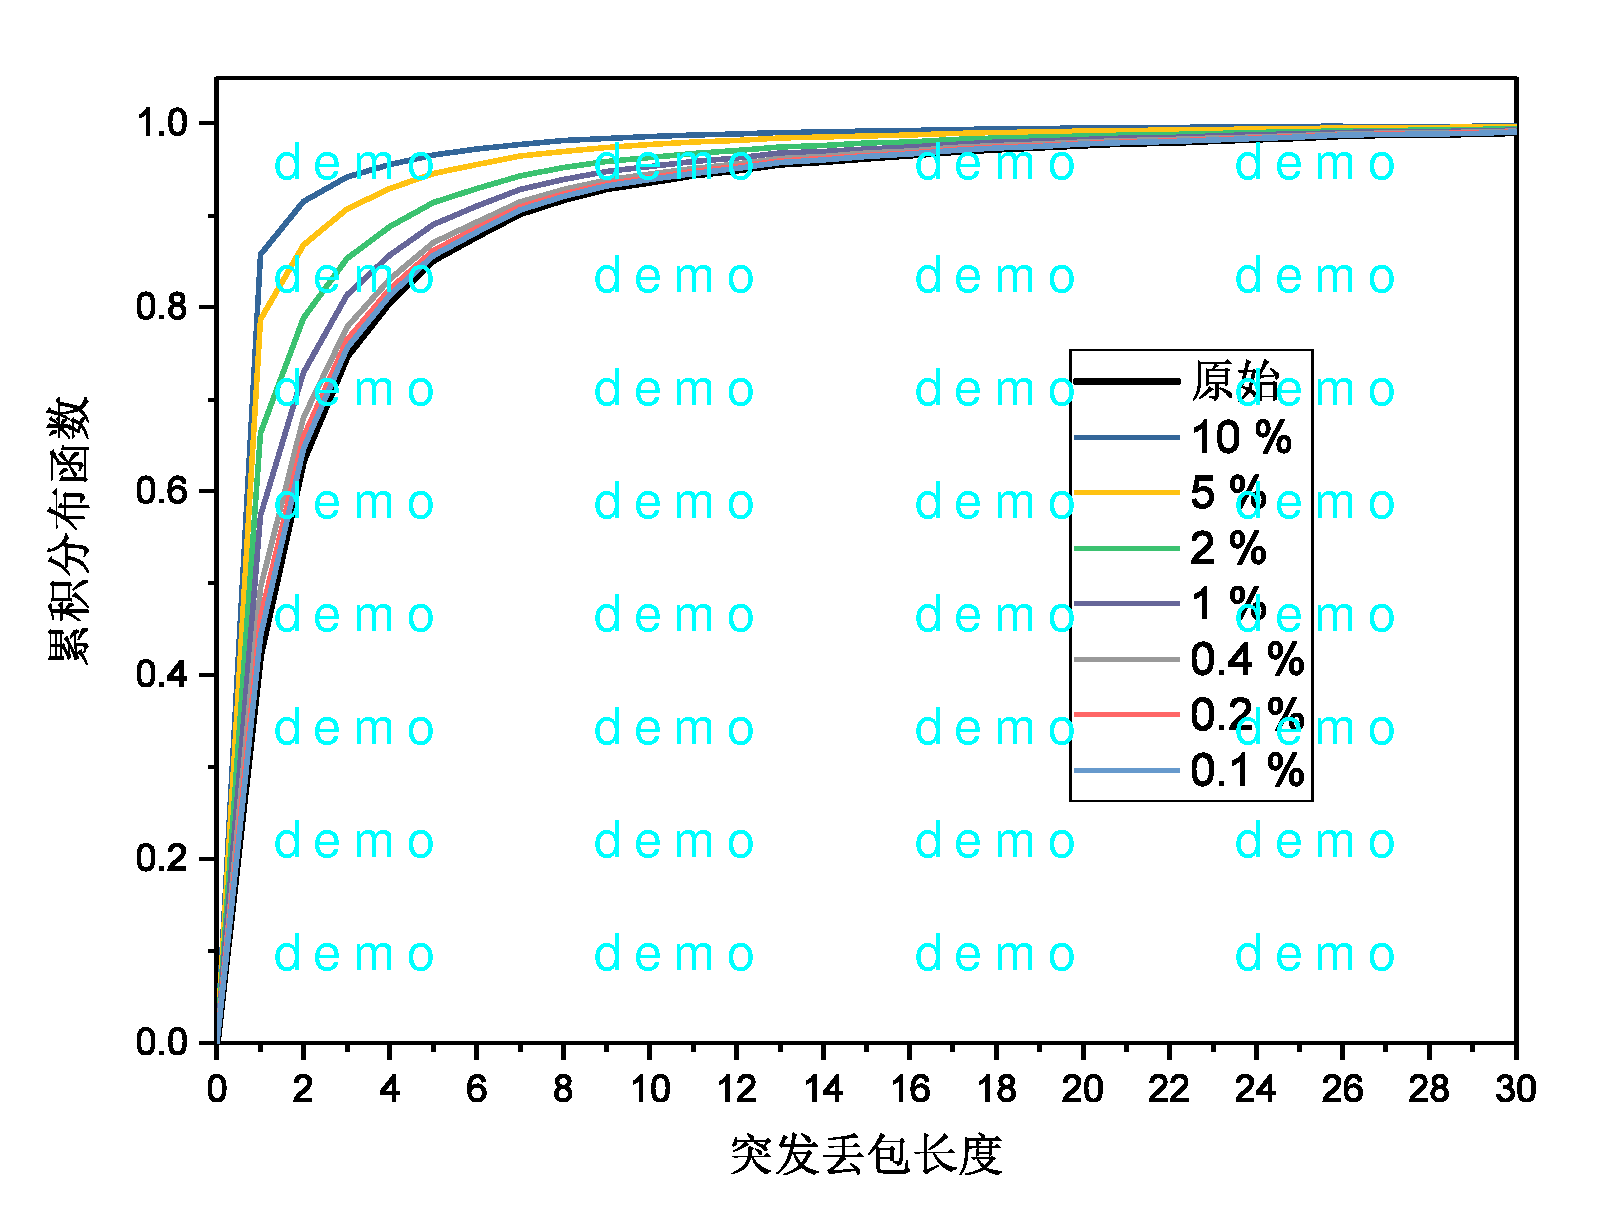
\includegraphics[width=0.48\textwidth]{chapters/chapter3/figures/burst-cdf-good.pdf}
        }
        \caption{连续丢包数的CDF曲线}
        \label{fig:3:result:burst:cdf}
	\end{figure}
}

如图\ \nref{fig:3:result:burst:cdf},时间隐通道对连续丢包数分布产生了影响。图\ \nref{fig:3:result:burst:cdf:excellent}Excellent场景中,随着主动丢包率的增加,曲线的上升趋势加快,偏离原始分布。图\ \nref{fig:3:result:burst:cdf:good}Good场景中,由于原始分布中已经存在较多的丢包,所以时间隐通道产生的影响较小,但对比原始分布,曲线上升趋势也发生改变。通过CDF判断,样本中存在时间隐通道的可能,需要进一步量化评估。

\subsubsection{条件熵检测结果}
\label{chap:analyze:result:burst:kld}

\insertFigure{
    \begin{figure}[htb]
        \centering
        \subfigure[Excellent场景K-L散度的箱线图]{
            \label{fig:3:result:burst:kld:excellent}
            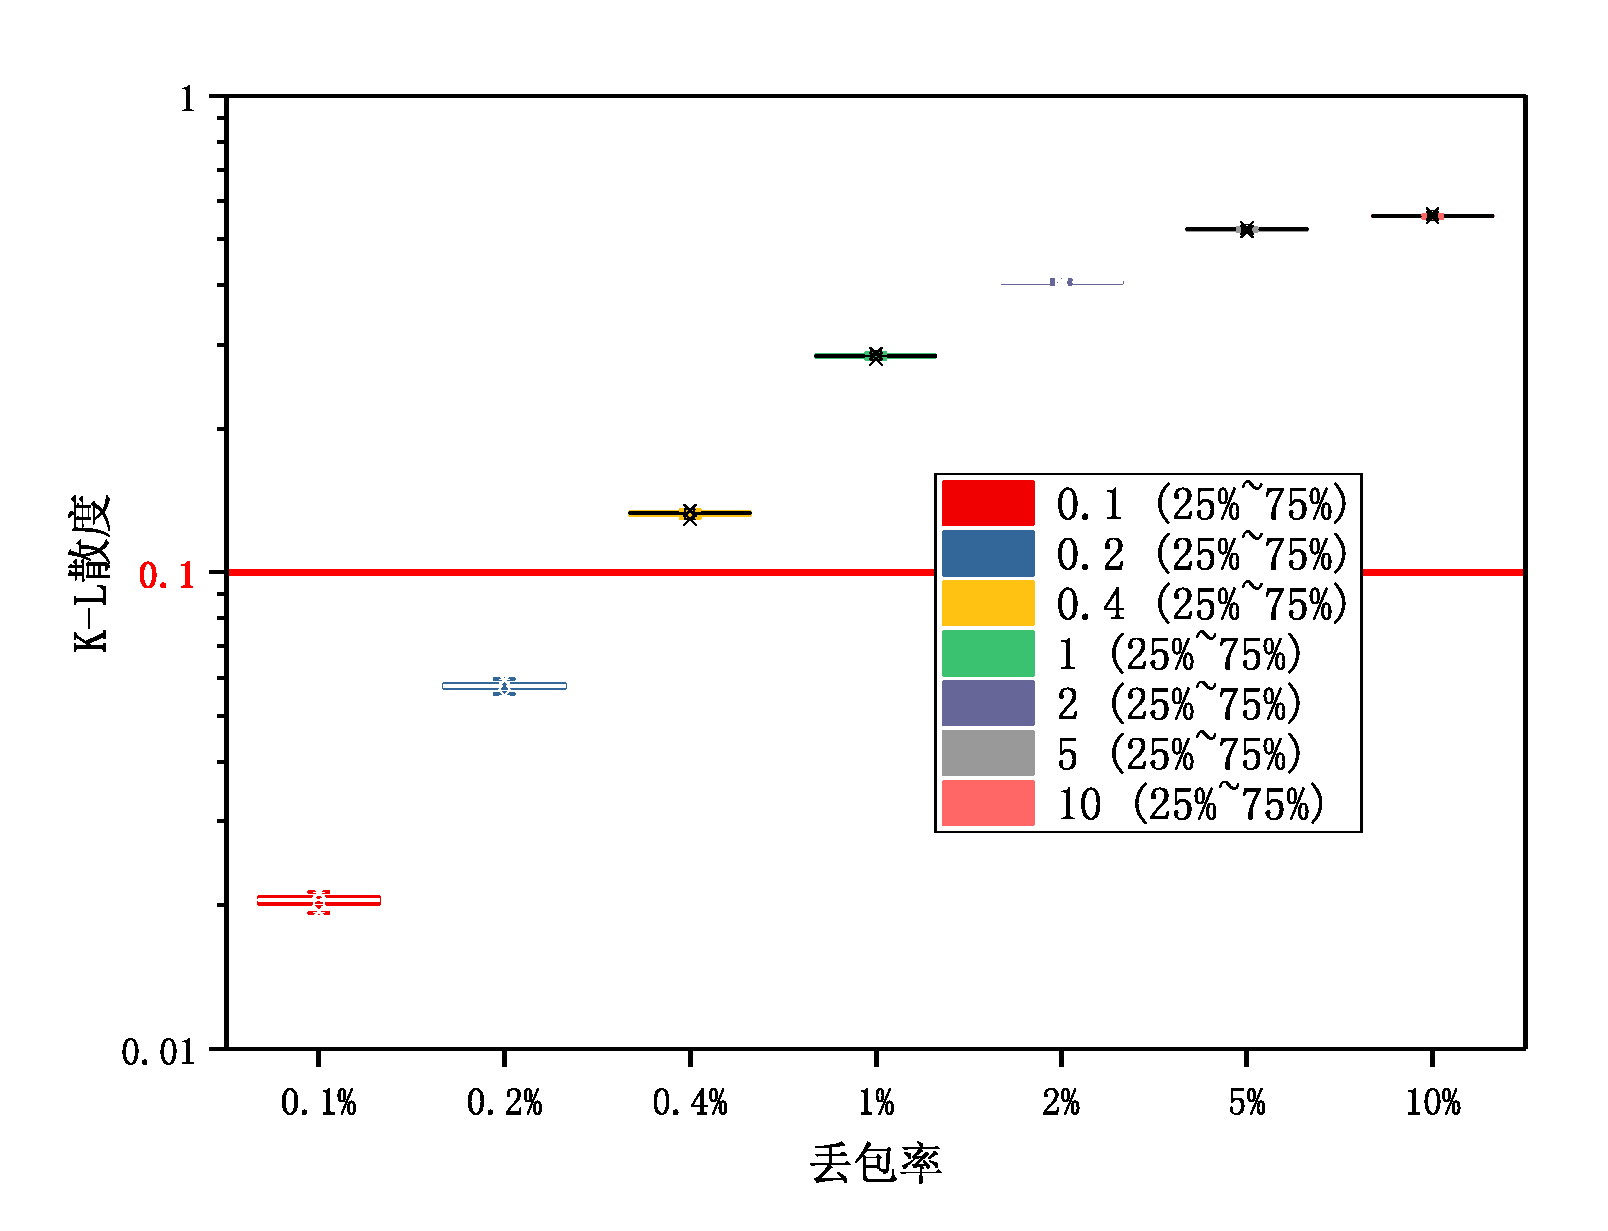
\includegraphics[width=0.48\textwidth]{chapters/chapter3/figures/burst-kld-excellent.pdf}
        }
        \subfigure[Good场景K-L散度的箱线图]{
            \label{fig:3:result:burst:kld:good}
            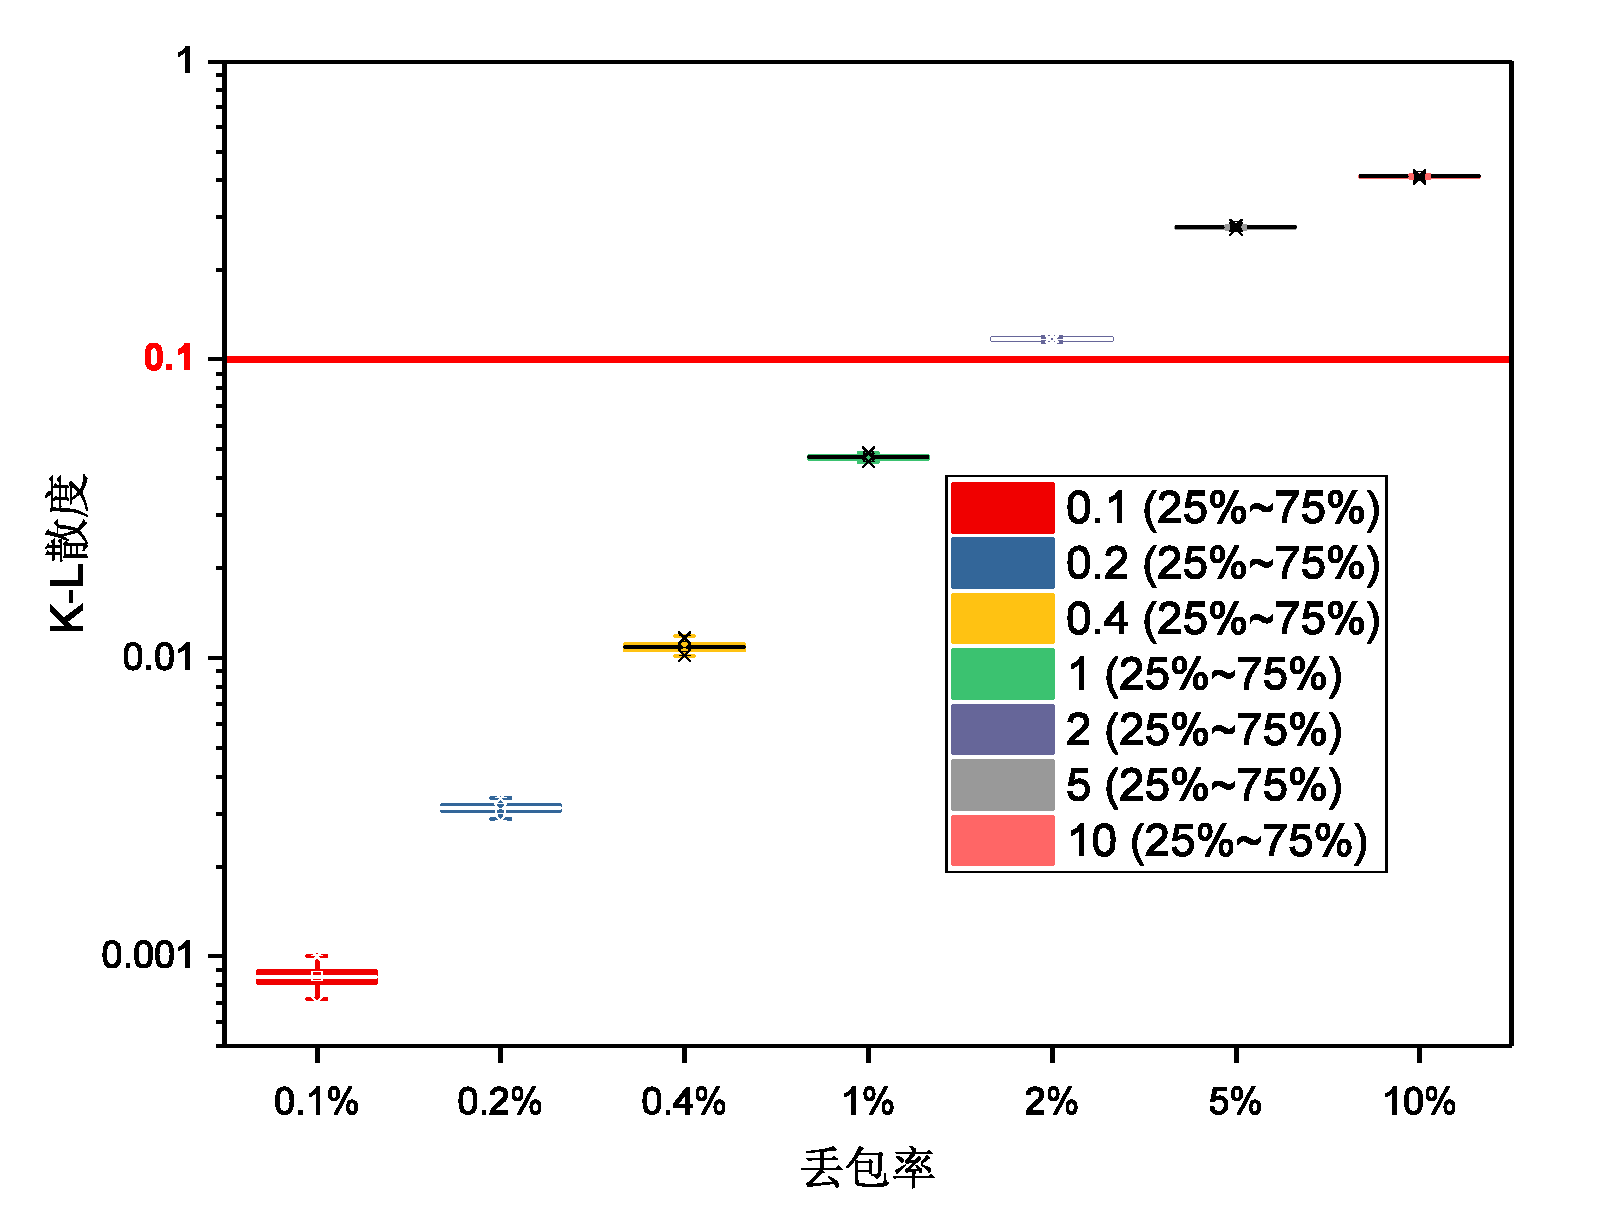
\includegraphics[width=0.48\textwidth]{chapters/chapter3/figures/burst-kld-good.pdf}
        }
        \caption{连续丢包数K-L散度检测的箱线图}
        \label{fig:3:result:burst:kld}
    \end{figure}
}

如图\ \nref{fig:3:result:burst:kld},通过K-L散度已经能够有效检测时间隐通道。图\ \nref{fig:3:result:burst:kld:excellent}Excellent场景中,只有主动丢包率$\le 0.2\%$时,才通过K-L散度检测。图\ \nref{fig:3:result:burst:kld:good}Good场景中,当主动丢包率$\le 1\%$时,即可通过K-L散度检测。检测结果表明,良好的网络条件中,对主动丢包时间隐通道的要求较高;而Good场景中,基于主动丢包的时间隐通道更容易隐蔽于网络噪声中。

\subsubsection{相对距离检测结果}
\label{chap:analyze:result:burst:distance}

\insertFigure{
	\begin{figure}[htb]
        \centering
        \subfigure[Excellent场景Wasserstein距离的箱线图]{
            \label{fig:3:result:burst:wd:excellent}
            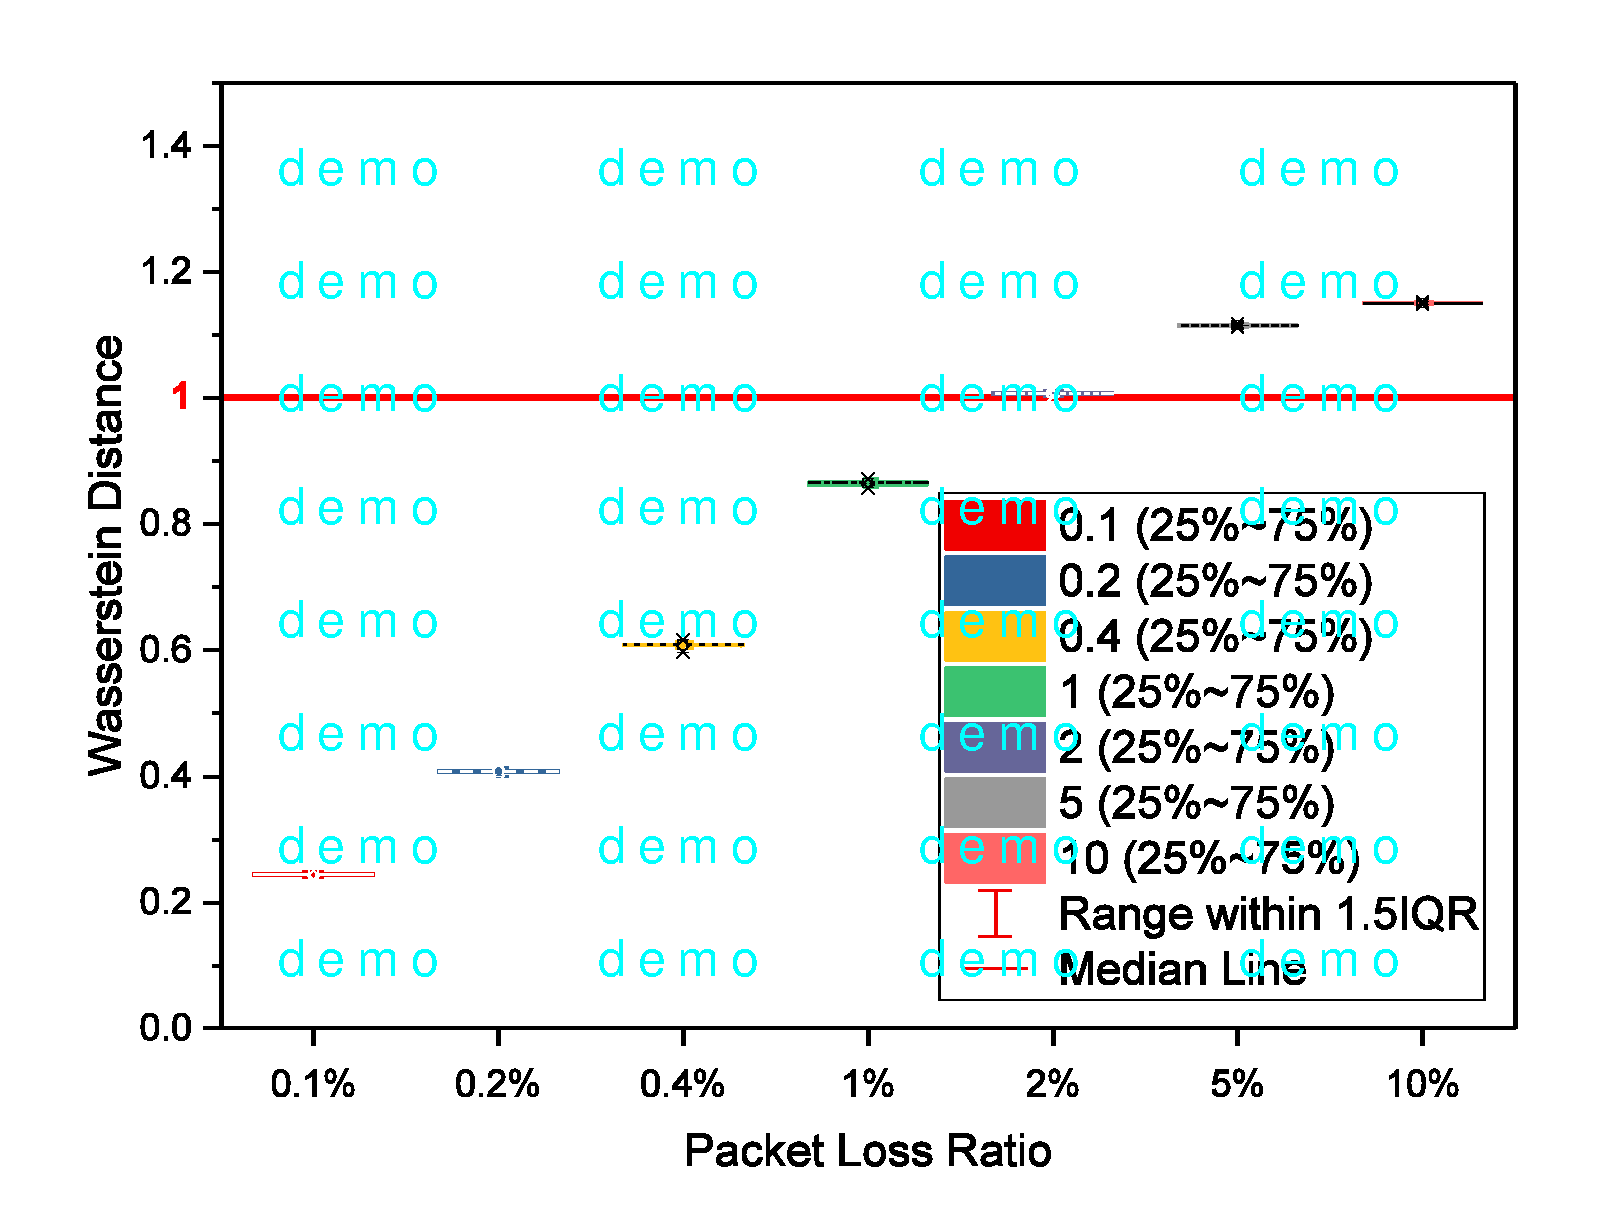
\includegraphics[width=0.48\textwidth]{chapters/chapter3/figures/burst-wd-excellent.pdf}
        }
        \subfigure[Good场景Wasserstein距离的箱线图]{
            \label{fig:3:result:burst:wd:good}
            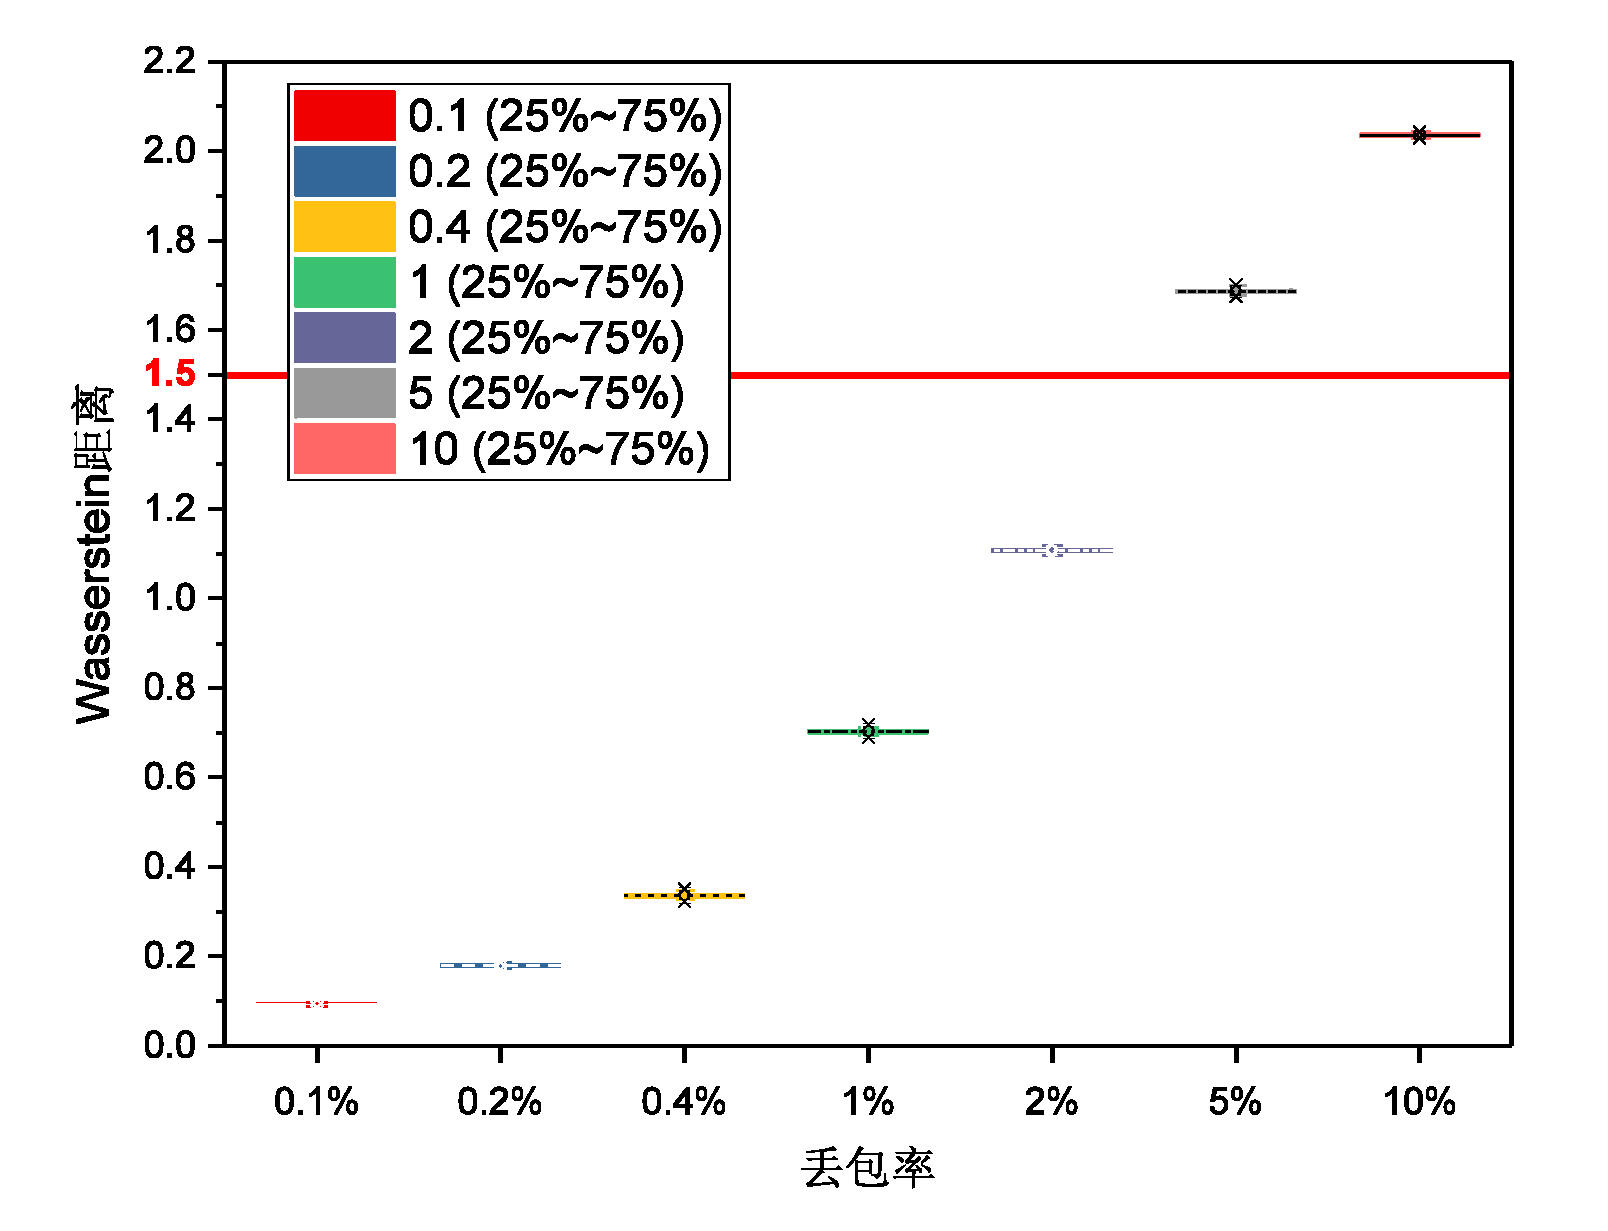
\includegraphics[width=0.48\textwidth]{chapters/chapter3/figures/burst-wd-good.pdf}
        }
        \caption{连续丢包数Wasserstein距离检测的箱线图}
        \label{fig:3:result:burst:wd}
	\end{figure}

	\begin{figure}[htb]
        \centering
        \subfigure[Excellent场景能量距离的箱线图]{
            \label{fig:3:result:burst:ed:excellent}
            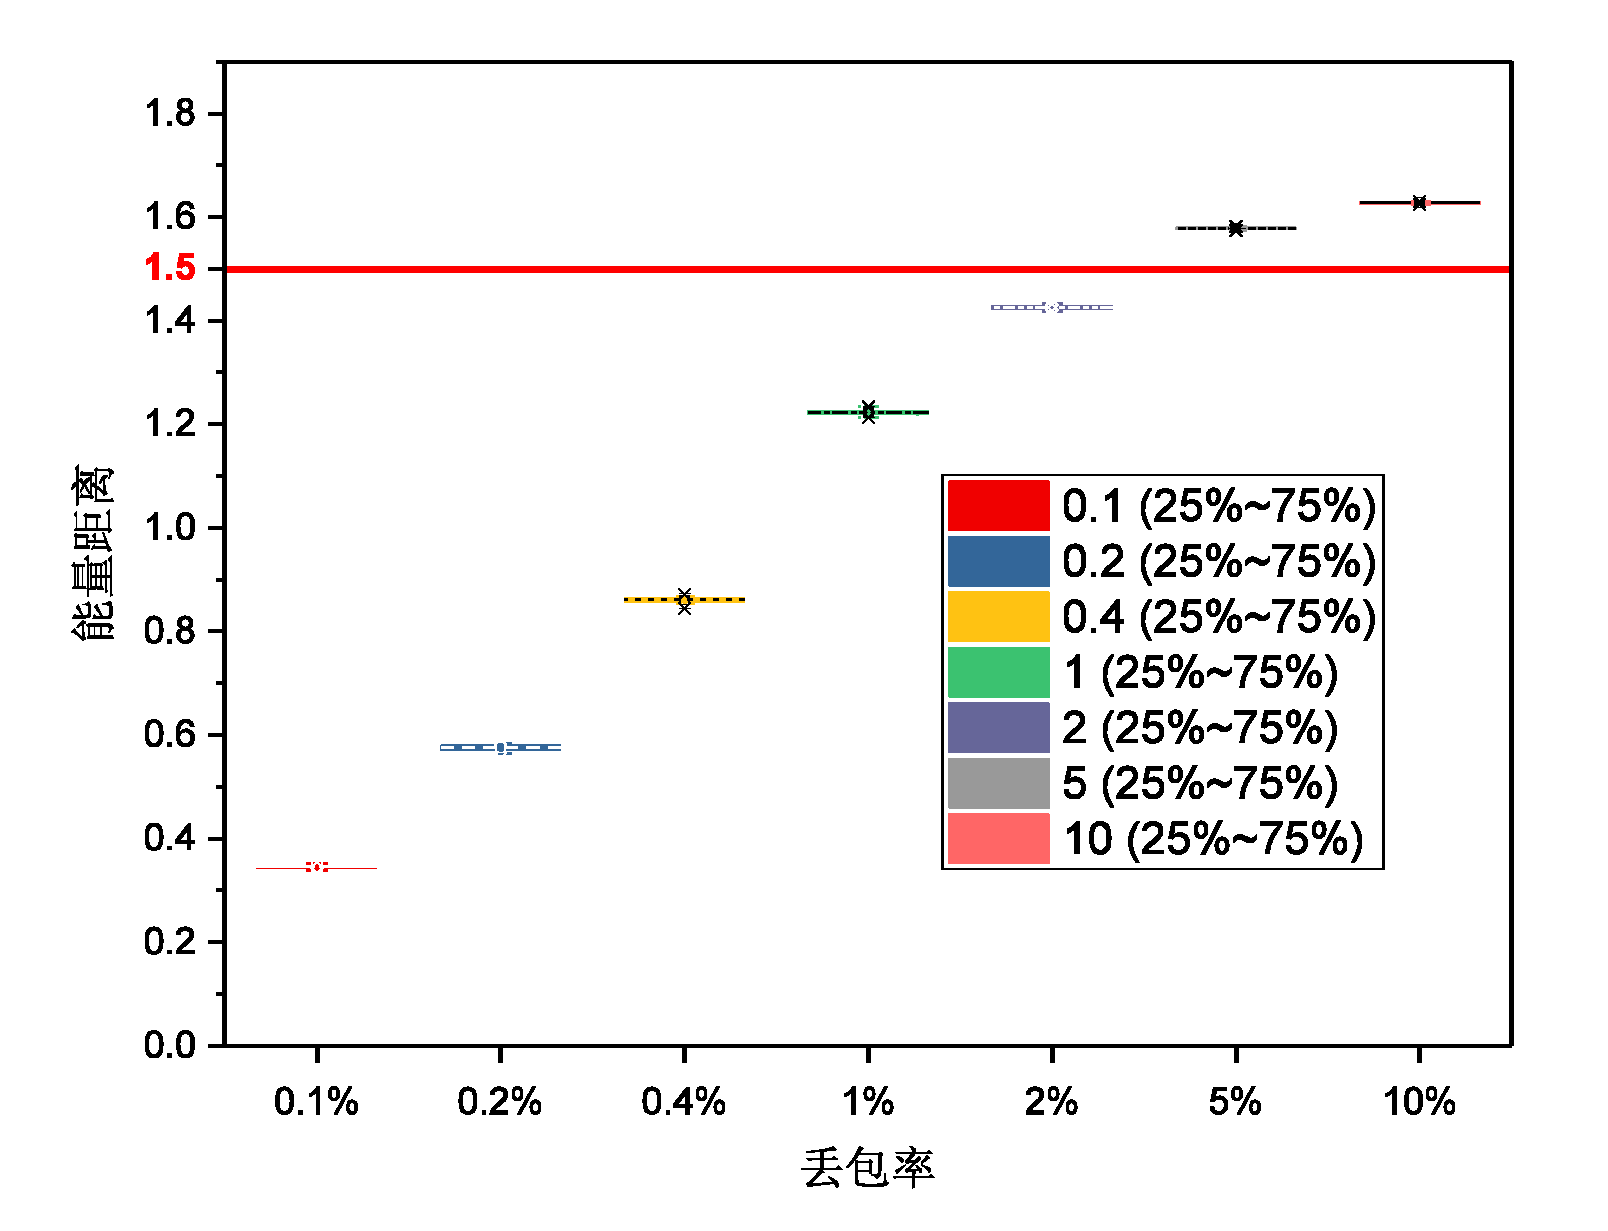
\includegraphics[width=0.48\textwidth]{chapters/chapter3/figures/burst-ed-excellent.pdf}
        }
        \subfigure[Good场景能量距离的箱线图]{
            \label{fig:3:result:burst:ed:good}
            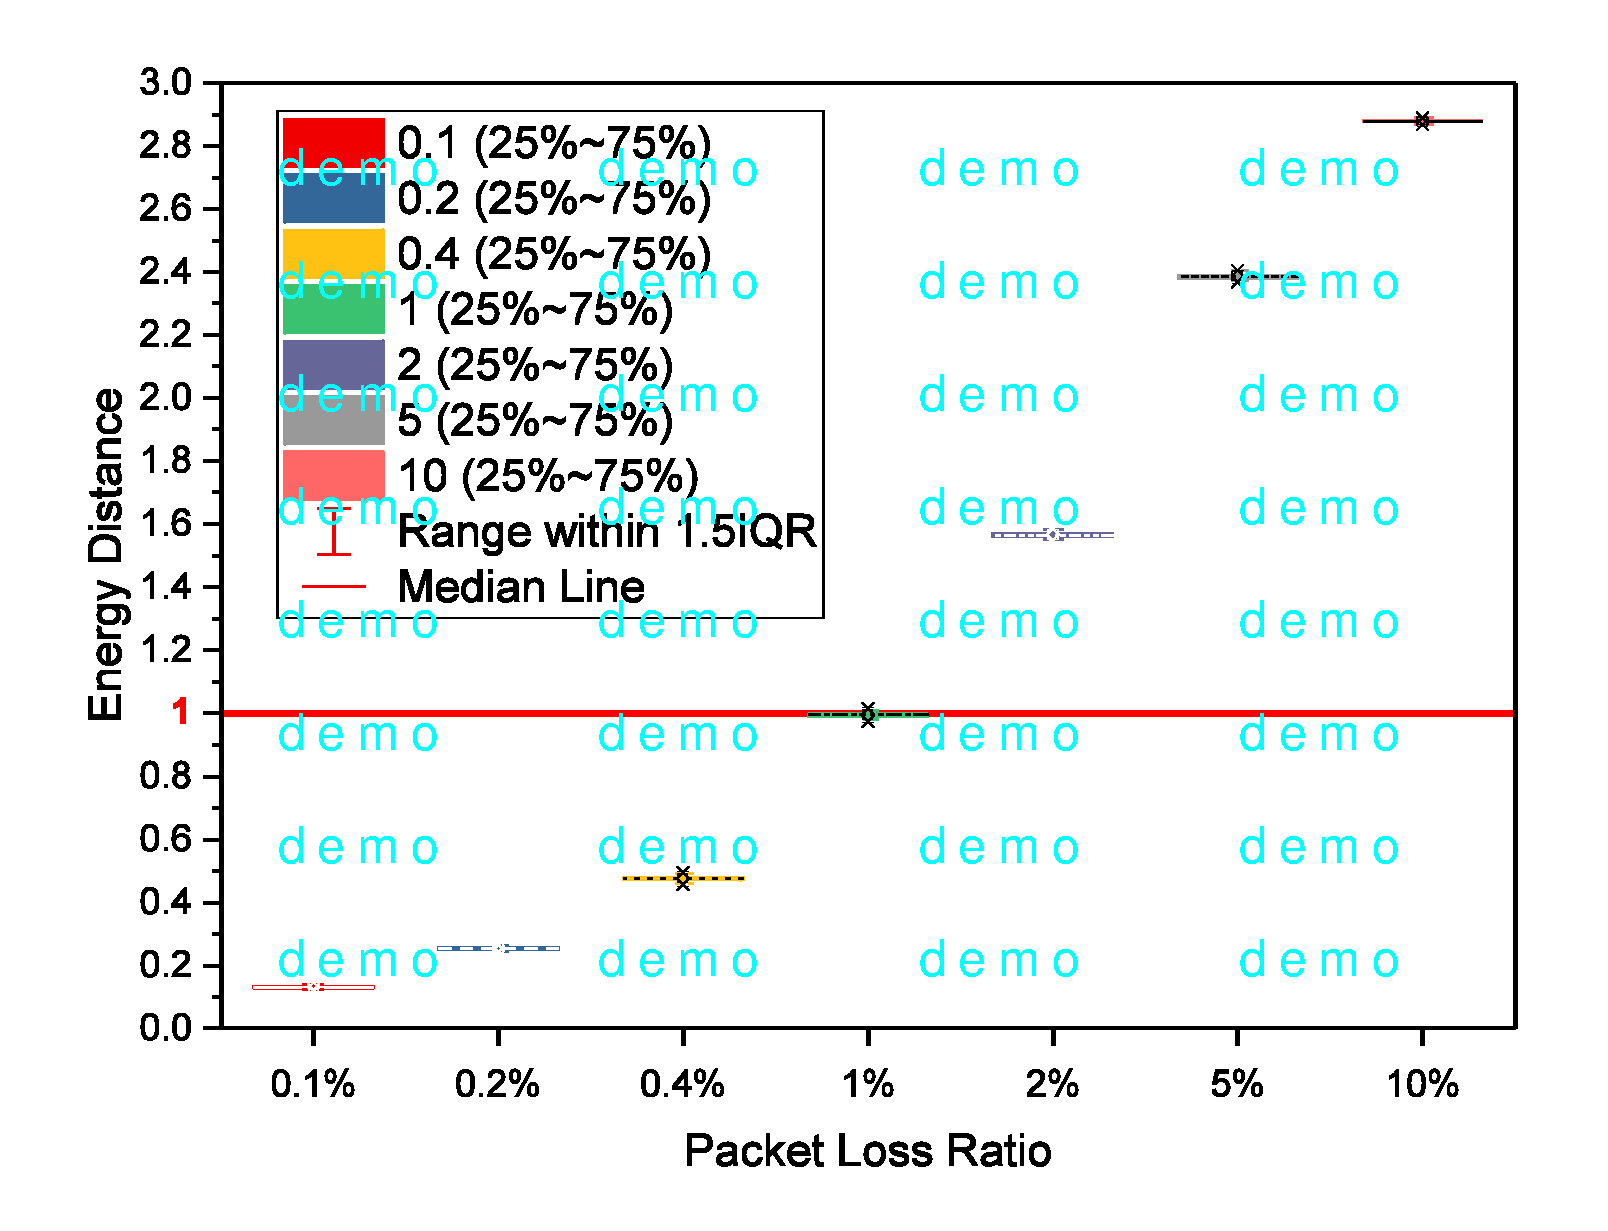
\includegraphics[width=0.48\textwidth]{chapters/chapter3/figures/burst-ed-good.pdf}
        }
        \caption{连续丢包数能量距离检测的箱线图}
        \label{fig:3:result:burst:ed}
	\end{figure}
}

如图\ \nref{fig:3:result:burst:wd},两种场景下Wasserstein距离检测结果总体一致。Excellent场景中,主动丢包率$\le 10\%$即可通过Wasserstein距离检测;而Good场景中,主动丢包率$\le 2\%$才通过检测。由于时间隐通道产生的连续丢包数为1,因此Good场景中的累积效应影响较大。

如图\ \nref{fig:3:result:burst:ed},能量距离检测结果与Wasserstein距离检测结果类似。Excellent场景下,主动丢包率$\le 2\%$即可通过检验;Good场景下,主动丢包率$\le 1\%$才通过检验。能量距离检测要求较Wasserstein更加严格,Good场景较Excellent场景更加严格。在相对距离检测中,检测结果具有较好区分度,并且与CDF曲线趋势一致,表明具有较好的检测能力。

对比本文\ \nref{chap:analyze:result:ipd}基于IPD的检测结果,基于连续丢包数分布的检测,已能能够有效检测基于主动丢包的时间隐通道。Excellent场景下,K-L散度具有更好的检测效果;Good场景下,相对距离检测的效果优于K-L散度检测。

\subsection{区间丢包数检测结果评估}
\label{chap:analyze:result:window}

如图\ \nref{fig:3:capture:win-cdf},不同区间长度设定下,区间丢包数随之变化。较小的区间长度有益于Excellent场景的检测,较大的区间长度有益于Good场景的检测。本检测中,区间长度设定为100及200。

\subsubsection{CDF检测结果}
\label{chap:analyze:result:window:cdf}

\insertFigure{
    \begin{figure}[htbp]
        \centering
        \subfigure[区间长度为100时Excellent场景的CDF曲线]{
            \label{fig:3:result:win100:cdf:excellent}
            \includegraphics[width=0.48\textwidth]{chapters/chapter3/figures/win100-cdf-excellent.pdf}
        }
        \subfigure[区间长度为100时Good场景的CDF曲线]{
            \label{fig:3:result:win100:cdf:good}
            \includegraphics[width=0.48\textwidth]{chapters/chapter3/figures/win100-cdf-good.pdf}
        }
        \subfigure[区间长度为200时Excellent场景的CDF曲线]{
            \label{fig:3:result:win200:cdf:excellent}
            \includegraphics[width=0.48\textwidth]{chapters/chapter3/figures/win200-cdf-excellent.pdf}
        }
        \subfigure[区间长度为200时Good场景的CDF曲线]{
            \label{fig:3:result:win200:cdf:good}
            \includegraphics[width=0.48\textwidth]{chapters/chapter3/figures/win200-cdf-good.pdf}
        }
        \caption{区间丢包数的CDF曲线}
        \label{fig:3:result:win:cdf}
	\end{figure}
}

如图\ \nref{fig:3:result:win:cdf},时间隐通道对CDF曲线产生了影响。对比图\ \nref{fig:3:result:win100:cdf:excellent}及图\ \nref{fig:3:result:win100:cdf:good},区间长度相同时,Excellent场景下的CDF曲线上升趋势更加迅速,意味着丢包数较少的区间占据的比例较高。对比图\ \nref{fig:3:result:win100:cdf:excellent}及图\ \nref{fig:3:result:win200:cdf:excellent},相同场景中增大区间长度后,曲线的上升趋势减缓,更有利于判断分布的差异。

对比CDF曲线,时间隐通道的主动丢包率越高,对分布曲线的影响越大。当主动丢包的间隔小于区间长度时,无丢包区间减少,CDF曲线中体现为起始位置偏移。因此,CDF曲线能够检测出主动丢包率$\ge 5\%$的时间隐通道。

\subsubsection{相对距离检测结果}
\label{chap:analyze:result:window:distance}

\insertFigure{
	\begin{figure}[htbp]
        \centering
        \subfigure[区间长度为100时Excellent场景的Wasserstein距离]{
            \label{fig:3:result:win100:wd:excellent}
            \includegraphics[width=0.48\textwidth]{chapters/chapter3/figures/win100-wd-excellent.pdf}
        }
        \subfigure[区间长度为100时Good场景的Wasserstein距离]{
            \label{fig:3:result:win100-wd:good}
            \includegraphics[width=0.48\textwidth]{chapters/chapter3/figures/win100-wd-good.pdf}
        }
        \subfigure[区间长度为200时Excellent场景的Wasserstein距离]{
            \label{fig:3:result:win200:wd:excellent}
            \includegraphics[width=0.48\textwidth]{chapters/chapter3/figures/win200-wd-excellent.pdf}
        }
        \subfigure[区间长度为200时Good场景的Wasserstein距离]{
            \label{fig:3:result:win200:wd:good}
            \includegraphics[width=0.48\textwidth]{chapters/chapter3/figures/win200-wd-good.pdf}
        }
        \caption{区间丢包数Wasserstein距离检测的箱线图}
        \label{fig:3:result:win:wd}
	\end{figure}

	\begin{figure}[htbp]
        \centering
        \subfigure[区间长度为100时Excellent场景能量距离的箱线图]{
            \label{fig:3:result:win100:ed:excellent}
            \includegraphics[width=0.48\textwidth]{chapters/chapter3/figures/win100-ed-excellent.pdf}
        }
        \subfigure[区间长度为100时Good场景能量距离的箱线图]{
            \label{fig:3:result:win100-ed:good}
            \includegraphics[width=0.48\textwidth]{chapters/chapter3/figures/win100-ed-good.pdf}
        }
        \subfigure[区间长度为200时Excellent场景能量距离的箱线图]{
            \label{fig:3:result:win200:ed:excellent}
            \includegraphics[width=0.48\textwidth]{chapters/chapter3/figures/win200-ed-excellent.pdf}
        }
        \subfigure[区间长度为200时Good场景能量距离的箱线图]{
            \label{fig:3:result:win200:ed:good}
            \includegraphics[width=0.48\textwidth]{chapters/chapter3/figures/win200-ed-good.pdf}
        }
        \caption{区间丢包数能量距离检测的箱线图}
        \label{fig:3:result:win:ed}
	\end{figure}
}

如图\ \nref{fig:3:result:win:wd},区间长度为100时,只有主动丢包率$\le 1\%$才通过Wasserstein距离检测;而区间长度扩展到200时,只有主动丢包率$\le 0.4\%$才通过检测。如图\ \nref{fig:3:result:win:ed},能量距离检测结果类似Wasserstein距离检测结果,当区间长度为100时,主动丢包率$\le 1\%$才通过检测;而区间长度为200时,主动丢包率$\le 0.4\%$才有较高的几率通过检测。

\subsection{总结}
通过分析检测结果,相对距离有效反映了CDF曲线的差异,结合K-L散度得到更全面的检测结果。实验结果证明,结合区间丢包数分布和连续丢包数分布后,有效补充了基于IPD的检测方法。根据表\ \nref{tab:3:detect-sum}中设定的10条量化评估子项,汇总得到最终的检出率表。

\insertTable{
	\begin{table}[htbp]
      \centering
      \caption{Excellent场景下时间隐通道检出率汇总表}
      \label{tab:3:result-sum:excellent}
        \begin{threeparttable}
          \begin{tabular*}{0.99\textwidth}{@{\extracolsep{\fill}}ccccccccc}
            \toprule
            对象 & 方法 & 10\% & 5\% & 2\% & 1\% & 0.4\% & 0.2\% & 0.1\%\\ 
            \midrule
            \multirow{5}{*}{IPD分布} & K-S检验 & 100\% & 100\% & 100\% & 0\% & 0\% & 0\% & 0\% \\
            & t检验,rank检验\tnote{1} & 100\% & 100\% & 100\% & 100\% & 0\% & 0\% & 0\% \\
            & K-L散度 & 0\% & 0\% & 0\% & 0\% & 0\% & 0\% & 0\% \\
            & Wasserstein距离 & 0\% & 0\% & 0\% & 0\% & 0\% & 0\% & 0\% \\
            & 能量距离 & 100\% & 0\% & 0\% & 0\% & 0\% & 0\% & 0\% \\
            \\
            \multirow{3}{*}{连续丢包数} & K-L散度 & 100\% & 100\% & 100\% & 100\% & 100\% & 0\% & 0\% \\
            & Wasserstein距离 & 0\% & 0\% & 0\% & 0\% & 0\% & 0\% & 0\% \\
            & 能量距离 & 100\% & 100\% & 0\% & 0\% & 0\% & 0\% & 0\% \\
            \\
            \multirow{2}{*}{区间丢包数} & Wasserstein距离 & 100\% & 100\% & 100\% & 100\% & 0\% & 0\% & 0\% \\
            & 能量距离 & 100\% & 100\% & 100\% & 100\% & 0\% & 0\% & 0\% \\
            \bottomrule
          \end{tabular*}
          \begin{tablenotes}
            \footnotesize
            \item[1] Welch's t检验与Mann–Whitney rank检验通过一种即可
          \end{tablenotes}
        \end{threeparttable}
    \end{table}
}

\insertTable{
	\begin{table}[htbp]
      \centering
      \caption{Good场景下时间隐通道检出率汇总表}
      \label{tab:3:result-sum:good}
        \begin{threeparttable}
          \begin{tabular*}{0.99\textwidth}{@{\extracolsep{\fill}}ccccccccc}
            \toprule
            对象 & 方法 & 10\% & 5\% & 2\% & 1\% & 0.4\% & 0.2\% & 0.1\%\\ 
            \midrule
            \multirow{5}{*}{IPD分布} & K-S检验 & 100\% & 100\% & 100\% & 0\% & 0\% & 0\% & 0\% \\
            & t检验,rank检验\tnote{1} & 100\% & 100\% & 0\% & 0\% & 0\% & 0\% & 0\% \\
            & K-L散度 & 0\% & 0\% & 0\% & 0\% & 0\% & 0\% & 0\% \\
            & Wasserstein距离 & 0\% & 0\% & 0\% & 0\% & 0\% & 0\% & 0\% \\
            & 能量距离 & 100\% & 0\% & 0\% & 0\% & 0\% & 0\% & 0\% \\
            \\
            \multirow{3}{*}{连续丢包数} & K-L散度 & 100\% & 100\% & 100\% & 0\% & 0\% & 0\% & 0\% \\
            & Wasserstein距离 & 100\% & 100\% & 0\% & 0\% & 0\% & 0\% & 0\% \\
            & 能量距离 & 100\% & 100\% & 100\% & 0\% & 0\% & 0\% & 0\% \\
            \\
            \multirow{2}{*}{区间丢包数} & Wasserstein距离 & 100\% & 100\% & 100\% & 100\% & 11\% & 0\% & 0\% \\
            & 能量距离 & 100\% & 100\% & 100\% & 100\% & 11\% & 0\% & 0\% \\
            \bottomrule
          \end{tabular*}
          \begin{tablenotes}
            \footnotesize
            \item[1] Welch's t检验与Mann–Whitney rank检验通过一种即可
          \end{tablenotes}
        \end{threeparttable}
    \end{table}
}

如表\ \nref{tab:3:result-sum:excellent}及表\ \nref{tab:3:result-sum:good},不同方法的检出率存在差异,不同场景的检出率也存在差距。Excellent场景中,连续丢包数及区间丢包数的检测,能够准确体现主动丢包的影响。当主动丢包的比例降低,超过了检测方法的灵敏度,时间隐通道将无法被检测出来。Good场景中,由于信道中已经存在一定比例的丢包事件,连续丢包数的检测能力减弱;但基于区间丢包数的检测方法,能够进一步区分随机丢包,因此具有较好的检测效果。

\insertTable{
	\begin{table}[htbp]
      \centering
      \caption{时间隐通道检出率汇总表}
      \label{tab:3:result-sum:all}
          \begin{tabular*}{0.99\textwidth}{@{\extracolsep{\fill}}cccccccc}
            \toprule
            \multirow{2}{*}{场景} 
            & \multicolumn{7}{c}{主动丢包率} \\
            \cmidrule(l){2-8}
            & 10\% & 5\% & 2\% & 1\% & 0.4\% & 0.2\% & 0.1\% \\ 
            \midrule
            Excellent & 100\% & 100\% & 100\% & 100\% & 100\% & 0\% & 0\% \\
            Good & 100\% & 100\% & 100\% & 100\% & 11\% & 0\% & 0\% \\
            \bottomrule
          \end{tabular*}
    \end{table}
}

汇总所有检测子项的结果,时间隐通道检测能力如表\ \nref{tab:3:result-sum:all}。由表可知,该检测方法对主动丢包敏感,只有时间隐通道的主动丢包率控制在$0.4\%$以下,才有可能通过检测。
\section{本章小结}
\label{chap:analyze:summary}

\chapter{基于Zigzag映射矩阵的时间隐通道构建方法}
\label{chap:zigzag}

本章介绍的是基于Zigzag映射矩阵的时间隐通道构建方法,通过离散丢包的方式,丢弃具有特定数据包序号的数据包,实现隐蔽消息嵌入操作。由于RTP的数据包序号存在唯一性,发送方产生的主动丢包时间一定可以被接收方观测。接受方监听丢失的数据包序号,并根据鲁棒性方法去除噪声,便可得到隐蔽消息,完成时间隐通道的传输。基于Zigzag映射矩阵,实现了时间隐通道中码字到符号的映射,解除了码字与符号之间的线性关联。

%在下方加入各小节内容
\section{概述}
\label{chap:zigzag:overview}

根据时间隐通道的构建指标,时间隐通道应满足抗检测能力、鲁棒性、传输性能、构建代价及保密性方面的要求。VoLTE中基于主动丢包的时间隐通道,能够满足抗检测能力的约束,构建方法需要满足其余指标。因此在该构建方法中,通过结合Zigzag映射矩阵提高鲁棒性及保密性。

在鲁棒性方面,通过添加校验码字并结合Zigzag映射矩阵,将噪声影响离散化并通过验证校验实现去噪。借助CRC校验的确定性和随机性,调制过程中建立数据码字与校验码字的匹配关系,解调过程中通过重新验证校验关系区分噪声。

%该方法的创新点
该方法的创新点如下:
\begin{itemize}
	\item 提出了基于Zigzag映射矩阵的时间隐通道构建方法,并且具有足够的抗检测能力及鲁棒性;
	\item 基于Zigzag映射矩阵,建立了符号与码字之间的非线性映射;
	\item 引入了RTP中的随机字段,增加传输过程的随机化,增强隐蔽消息的保密性。
\end{itemize}

经实验验证,该时间隐通道在满足抗检测性的前提下,保证了一定的传输能力,满足了时间隐通道构建指标的要求。
\section{研究背景和动机}
\label{chap:zigzag:motivation}

本章主要介绍研究背景及研究动机,主要包括基于主动丢包的时间隐通道可行性分析,对Zigzag矩阵应用在码字-符号转换中的意义,及CRC校验如何提高时间隐通道的鲁棒性几个方面。结合\nref{chap:backinfo}对时间隐通道,及VoLTE视频通话场景的信道分析,参照\nref{chap:analyze}部分时间隐通道检测方法的测试,充分利用时间隐通道的构建基础,设计具有实际应用价值的构建方法,是本章的主要工作。

\subsection{基于主动丢包构建时间隐通道}
\label{chap:zigzag:motivation:dropout}
如图\nref{fig:2:pmf-dropout},VoLTE网络噪声中,长度为1的离散丢包占据总量的50\%左右。并且经过\nref{chap:analyze:result}实验的检验,当时间隐通道的主动丢包率降低到一定程度,即可规避现有的检测方法。因此,基于主动丢包的时间隐通道,在基本构造原理上依然可行。

对于隐通道的通信双方来说,如何有效识别数据包是一个非常重要的问题。在VoLTE中,可以有效利用RTP头中的Sequence Number字段,识别一次通话中数据包的唯一性。如图\nref{fig:2:rtp-header},数据包序号字段占据16 bit,最大可达到65536。正如\nref{chap:backinfo:rtp:dropout}对RTP丢包处理的描述,Sequence Number字段的作用,是识别一次通话中的数据包顺序,按照正确的顺序将负载提供给应用层。

基于数据包序号构建基于主动丢包的时间隐通道,具有以下优势:
\begin{itemize}
    \item 数据包序号具有传输同步能力,隐通道的传输过程以序号为参照时钟,无需时钟参照,简化了传输流程;
    \item 主动丢包行为不依赖数据包顺序,网络噪声中的乱序无法影响隐通道鲁棒性,防守方的数据包重排序也无法破坏隐通道;
    \item 防守方在防御时需要考虑对用户体验的影响,因此构造数据包填充丢包位置,对用户来说是可察觉的异常现象,一定程度上保证了丢包位置的传递;
    \item 如果防守反对数据包序号字段进行了覆写,则时间戳增长的线性关系被破坏,接收方可以监测到异常,并终止会话。
\end{itemize}

\subsection{ZigZag矩阵及其特征}
\label{chap:zigzag:motivation:zigzag}

\insertFigure{
	\begin{figure}
		\centering
        \includegraphics[width=0.6\textwidth]{chapters/chapter4/figures/zigzag-matrix.pdf}
        \caption{$8\times 8$的Zigzag矩阵示意图}
        \label{fig:4:zigzag-matrix}
	\end{figure}
}

Zigzag矩阵的排布方式,区别于常见的行优先或列优先,采用的是对角线折返的方式,不具备明显的线性关系。\nupcite{ji2015a,zaidee2006content,yang2018adaptive,li2019a}如图\nref{fig:4:zigzag-matrix}所示,矩阵中元素的坐标$(x,y)$,与元素的对应关系,由矩阵的规模决定。对于$L_{Codeword}=8$的时间隐通道来说,码字可以按照4 bit切分为上半部及下半部。参照Zigzag映射矩阵的定义,$(Codeword_{4~7},Codeword_{0~3})$可以对应到序号$Symbol$。

另一方面,Zigzag矩阵作为映射矩阵,其起始值支持用户设定,隐通道的双方可以约定一个安全的起始值,提高隐通道的保密性。即使防守方破解了隐通道的工作模式,并按照相同的解调方式,破解隐蔽消息,则需要对所有的可行解进行推测,提高了计算复杂度。随着矩阵规模的增大,矩阵中元素的排布关系会更加复杂,满足了隐通道的保密性要求。

\subsection{CRC数据校验策略}
\label{chap:zigzag:motivation:crc}

CRC是Cyclic Redundancy Check的缩写,全称为循环冗余校验码,在计算机网络及数据存储中有广泛应用。CRC作为散列函数的一种,可以生成数据的唯一摘要,根据位数的区别,常用的模式为CRC16及CRC32,更多的位数可以保证更低的冲突概率。在本时间隐通道中,CRC主要用于校验码字的正确性,无法使用全部的CRC校验值,因此,CRC16产生的结果可以基本满足校验的需求。

\insertFigure{
	\begin{figure}
		\centering
        \includegraphics[width=0.98\textwidth]{chapters/chapter4/figures/insert-crc.pdf}
        \caption{CRC校验添加模式示意图}
        \label{fig:4:insert-crc}
	\end{figure}
}

如图\nref{fig:4:insert-crc},在每个数据码字之后,追加一个校验码字,通过校验码字区分噪声及信号。在CRC的参数方面,除了当前待验证的码字,额外引入$Salt$变量,增加计算结果的随机性及保密性。$salt$由两部分组成,一部分是用户自定义的私有值,一部分是RTP数据包头中导出的随机字段。在掺杂网络噪声的场景中,借助散列函数的单向性,提高防守方破解隐蔽消息的难度及计算量。

\insertTable{
	\begin{table}[]
      \centering
      \caption{添加CRC校验后的码字密度表}
      \label{tab:4:codeword-density}
          \begin{tabular*}{0.98\textwidth}{@{\extracolsep{\fill}}ccccc}
            \toprule
            $L_{Codeword}$ (bit) & 码字及校验长度 (bit) & 数据包数 & 校验编码利用率 & 总体编码利用率 \\
            \midrule
            6 & 12 & 128 & 65.6\% & 83.6\% \\
            7 & 14 & 256 & 66.4\% & 82.4\% \\
            8 & 16 & 512 & 68.0\% & 81.1\% \\
            9 & 18 & 1024 & 64.5\% & 82.2\% \\
            10 & 20 & 2048 & 62.8\% & 81.3\% \\
            11 & 22 & 4096 & 62.9\% & 81.9\% \\
            12 & 24 & 8192 & 63.2\% & 81.8\% \\
            \bottomrule
          \end{tabular*}
    \end{table}
}

通过组合码字及CRC校验信息,等价于形成了一个超长码字,并且码字中自带校验信息。采取数据及校验分别传输的方式,能够有效提高码字的传输效率,同时保证信道资源的利用率。如表\nref{tab:4:codeword-density},按照一个数据码字对应一个校验码字的方式,传输一个码字,需要$2^{L_{Codeword}}\times 2$个数据包才能完成调制。由于在有限位数限制下,CRC摘要的结果只能截取$L_{Codeword}$ bit,因此,在传输校验码字中存在无法利用的编码位置,因此校验部分的编码利用率在65\%左右,总体的编码利用率在82\%左右。

\subsection{研究动机}
\label{chap:zigzag:motivation:conclude}
通过主动丢包的方式构建时间隐通道,最直接的方式是对数据包范围进行分片,每片中丢弃一个数据包,以数据包的相对位置代表隐蔽消息中的数据。但这种传输模式,在网络噪声干扰的情况下,无法确保接收方能够准确接收到隐蔽消息。此外,时间隐通道传输传输的都是隐蔽的敏感信息,直接的传输模式无法保证隐蔽消息的安全性,即使消息自身已经加密。

\insertFigure{
	\begin{figure}
		\centering
        \includegraphics[width=0.8\textwidth]{chapters/chapter4/figures/method-struct.pdf}
        \caption{基于Zigzag映射矩阵的时间隐通道研究要点与指标}
        \label{fig:4:method-struct}
	\end{figure}
}

本章所研究的构建方法,在分片调制的基础上,对每个分片内所传输数据的内容进行调整,提高抗噪声干扰能力。如图\nref{fig:4:method-struct},在鲁棒性方面基于CRC校验,在传输数据码字的过程中穿插校验码字,通过校验信息进行有效数据筛选。在抗检测性方面,参数设置支持不同的$L_{Codeword}$,在Excellent场景与Good场景中对应配置。在保密性方面,引入Zigzag映射矩阵,在码字与符号之间添加一层转换,并且配合初始化参数实现映射矩阵的随机化;同时,在计算CRC校验值时,添加盐值增加结果的随机程度,提高反向破解难度。
\section{基于Zigzag映射矩阵的时间隐通道构建方法}
\label{chap:zigzag:model}

本节对构建方法进行详细介绍,包括设计架构、调制流程及解调流程三个部分。设计架构部分,主要介绍该时间隐通道的主要流程,设计的处理环节及数据对象。调制流程部分,主要介绍调制过程中的流程、计算方法及数据处理流程。解调流程部分,主要介绍解调过程中,如何根据丢包序号还原隐蔽消息,包括数据转换及数据检验等部分。

\subsection{设计架构}
\label{chap:zigzag:model:system}

\insertFigure{
	\begin{figure}[htbp]
		\centering
        \includegraphics[width=0.98\textwidth]{chapters/chapter4/figures/system-model.pdf}
        \caption{基于Zigzag映射矩阵的时间隐通道系统模型图}
        \label{fig:4:system-model}
	\end{figure}
}

如图\nref{fig:4:system-model},对于用户Alice和Bob,希望通过该时间隐通道传输隐蔽消息,而监听者对两人的所有通信进行了监听,只允许进行被监听的VoLTE通话。在进行传输前,接收方与发送方预先约定一个私有的$Key$及$Salt$,类似消息加密的私有秘钥,用于CRC校验生成及映射矩阵初始化。调制过程的消息分组阶段,完成对隐蔽消息的分组,生成定长的消息块$D_{i}$。校验码字计算阶段依赖CRC算法,结合私有$Salt$及宿主信道中提取的随机信息,计算每个码字的校验值,生成所有码字$C_{j}$。码字-符号映射阶段,利用私有$Key$及随机信息初始化映射矩阵,将码字$C_{j}$映射到相对序号$S_{j}$。主动丢包阶段,监控当前的数据包传输状态,并将目标数据包直接丢弃。

VoLTE数据包经LTE网络传输后,时间隐通道与网络噪声叠加。接收方监听到达的RTP数据包序号,并记录下丢失数据包的序号。按照调制过程的逆序,解调过程识别获取的符号$S_{j}^{'}$,然后参照逆映射矩阵将符号$S_{j}^{'}$转换为码字$C_{j}^{'}$,逆映射时映射矩阵的初始化参数与调制阶段保持一致。有效码字鉴别阶段根据CRC校验码字,筛选出符合校验规则的数据块$D_{i}^{'}$。最终消息重组阶段组合所有的消息块,得到隐蔽消息。

\subsection{调制流程}
\label{chap:zigzag:model:modulation}

\insertFigure{
	\begin{figure}[htb]
		\centering
        \includegraphics[width=0.8\textwidth]{chapters/chapter4/figures/modulation-flow.pdf}
        \caption{基于Zigzag映射矩阵的时间隐通道调制流程}
        \label{fig:4:modulation-flow}
	\end{figure}
}

如图\nref{fig:4:modulation-flow},调制过程中的处理步骤可以分为四个阶段,与系统模型中的各阶段对应。待发送的隐蔽消息为输入变量,最终结果为具有序号$S_{j}$的数据包被丢弃。

\subsubsection{隐蔽消息分组}
\label{chap:zigzag:model:modulation:segment}
隐蔽消息按照参数$BL$,切分为定长的消息块$D_{i}$,每个消息块单独调制。相对丢包位置与消息块长度匹配,则传输每个符号需要的数据包数量为$2^{BL}$。对于本方法,码字中没有额外的校验信息,因此$L_{Codeword}=BL$。

\insertEquation{
    \begin{equation}
    \label{equ:4:throughput}
    \begin{split}
        Throughput\ &=\ \frac{L_{Codeword}}{2^{L_{Codeword}}}\ \times\ 100\quad (bps)\ \\
        &=\ \frac{BL}{2^{BL}}\ \times\ 100\quad (bps)
    \end{split}
    \end{equation}
}

当确定了传输参数$L_{Codeword}$,则该时间隐通道的传输性能可以通过公式(\nref{equ:4:throughput})计算,VoLTE视频数据包传输速率按照平均值$100\ (pkts/s)$计算。在有限的通话时间中,数据包总量是有限的,时间隐通道必须提高传输效率。在分组传输模式下,通信双方不需要同步时钟,提高了资源利用率。

\subsubsection{基于CRC的码字校验}
\label{chap:zigzag:model:modulation:crc}

计算CRC校验,需要结合用户自定义的私有$Salt$,以及由RTP传输流中导出的随机字段。在这里,选择RTP包头中的$SSRC$,与$Salt$进行异或后与消息块$D_{i}$进行拼接,共同作为CRC函数的参数。计算过程的描述如算法\nref{alg:4:codeword-generation},输入参数包括隐蔽消息及参数,最终返回生成的码字序列$C$。

\insertContents{
    \begin{algorithm}[htbp]
        \renewcommand{\algorithmcfname}{算法}
        \caption{码字生成}
        \label{alg:4:codeword-generation}
        \LinesNumbered
        \KwIn{$Covert\ Message,\ SSRC,\ Salt,\ L_{Codeword}$}
        \KwOut{$C\ \leftarrow\ \{\}$}
        $D\ \leftarrow\ \{\},\ offset\ \leftarrow\ 0$ \\
        \For {$offset\ <\ length(Covert\ Message)$} {
            $D_{i}\ \leftarrow\ Covert\ Message[offset\ :\ L_{Codeword}]$ \\
            append $\ D_{i}\ $ to $\ D$
        }
        $salt\ \leftarrow\ Salt\ \oplus\ SSRC$ \\
        \For {$D_i\ $ in $\ D$} {
            $C_{j}\ \leftarrow\ $CRC16\ ($salt\ //\ D_{i}\ //\ salt$) \\
            append $\ D_{i}\ $ to $\ C_{j}$ \\
            append $\ C_{j}\ $ to $\ C$
        }
        \Return $C$
    \end{algorithm}
}

\subsubsection{基于Zigzag的映射矩阵}
\label{chap:zigzag:model:modulation:mapping}

映射矩阵实现了码字$C_{j}$到符号$S_{j}$的转换,矩阵中元素数量由$L_{Codeword}$决定。矩阵的行数与列数如公式(\nref{equ:4:matrix-length})计算,映射矩阵$\textit{\textbf{M}}$为方阵,且满足$M_{cols}\times M_{rows}=2^{L_{Codeword}}$。映射矩阵的映射关系,是本方法保密性的重要环节。图\nref{fig:4:zigzag-matrix}中$M_{1,\ 1}$由1开始排布,而实际应用中,$M_{1,\ 1}$由用户设定的$Key$及RTP中的随机字段决定,计算公式如公式(\nref{equ:4:matrix-begin})。映射矩阵排布完毕后,对每个元素$\textit{\textbf{M}}_{i,\ j}$取模,确保不超过上限$2^{L_{Codeword}}$。

\insertEquation{
    \begin{equation}
    \label{equ:4:matrix-length}
		M_{cols}\ =\ M_{rows}\ =\ 2^{\frac{L_{Codeword}}{2}}
    \end{equation}
    \begin{equation}
    \label{equ:4:mapping}
        S_{j}\ =\ \textit{\textbf{M}}_{C_{j,\ \lbrack L_{Codeword}/2,\ L_{Codeword})},\ C_{j,\ \lbrack 0,\ L_{Codeword}/2)}}
    \end{equation}
    \begin{equation}
    \label{equ:4:matrix-begin}
    \textit{\textbf{M}}_{1,\ 1}\ =\ (Key\ \oplus\ SSRC)\ \%\ 2^{L_{Codeword}}\ +\ 1
    \end{equation}
}

码字转换为符号的过程,由映射矩阵实现。对于码字$C_{j}$,其整体长度为$L_{Codeword}$\ bits,按照$L_{Codeword}/2$\ bits进行划分,得到前半部分$C_{j,\ [0,\ L_{Codeword}/2)}$,以及后半部分$C_{j,\ [L_{Codeword}/2,\ L_{Codeword})}$。参照图\nref{fig:4:zigzag-matrix}及映射矩阵实现,按照公式(\nref{equ:4:mapping})完成转换。

\subsection{解调流程}
\label{chap:zigzag:model:demodulation}

\insertFigure{
	\begin{figure}[htb]
		\centering
        \includegraphics[width=0.8\textwidth]{chapters/chapter4/figures/demodulation-flow.pdf}
        \caption{基于Zigzag映射矩阵的时间隐通道解调流程}
        \label{fig:4:demodulation-flow}
	\end{figure}
}

如图\nref{fig:4:demodulation-flow},解调流程主要分为四个部分,分别为监听丢包序号、符号-码字逆映射、鉴别有效码字,以及消息重组。由于网络噪声不可避免,解调过程中每组的候选项不唯一,在完成验证前,所有的候选项都视为可行解。

\insertEquation{
    \begin{equation}
    \label{equ:4:group-id}
		j\ =\ \left \lfloor\frac{number\ -\ 1}{2^{L_{Codeword}}}\right \rfloor\ +\ 1
    \end{equation}
    \begin{equation}
    \label{equ:4:symbol}
        S_{j}\ =\ (number\ -\ 1)\ \%\ (2^{L_{Codeword}})\ +\ 1
    \end{equation}
}

根据映射矩阵的规模,每个矩阵对应的数据包数量为$2^{L_{Codeword}}$,则丢包序号$number$与$j$及$S_{j}$的对应关系如公式(\nref{equ:4:group-id})及公式(\nref{equ:4:symbol})。

\subsubsection{基于Zigzag矩阵的逆映射}
\label{chap:zigzag:model:demodulation:reverse-mapping}

映射矩阵将码字映射为符号,逆映射过程需要按照相同的规则还原码字。对于接收方来说,通过映射矩阵进行逆映射效率较低,需要首先生成映射矩阵的逆映射关系。按照调制过程相同的方式,在构建映射矩阵的过程中,创建逆映射关系$S_{j}\ \rightarrow\ C_{j}$,通过索引快速完成逆映射。

\subsubsection{有效码字鉴别}
\label{chap:zigzag:model:demodulation:identification}

\insertContents{
    \begin{algorithm}[htbp]
        \renewcommand{\algorithmcfname}{算法}
        \caption{有效码字鉴别}
        \label{alg:4:codeword-identification}
        \LinesNumbered
        \KwIn{$\{\{C_{1}',\ \cdots\},\ \{C_{2}',\ \cdots\},\ \cdots\},\ Salt,\ SSRC$}
        \KwOut{$D\ \leftarrow\ \{\}$}
        $salt\ \leftarrow\ Salt\ \oplus\ SSRC$ \\
        \For {$\{C_{j}',\ \cdots\},\ \{C_{j+1}',\ \cdots\}\ $ in $\ C$} {
            \For {$C_{j}'\ $ in $\ \{C_{j}',\ \cdots\}$} {
                $checksum\ =\ $CRC16\ ($salt\ //\ C_{j}'\ //\ salt$) \\
                \If {$checksum\ $ in $\ \{C_{j+1}',\ \cdots\}$} {
                    append $\ C_{j}'\ $ to $\ D$ \\
                    \textbf{break}
                }
            }
        }
        \Return $D$
    \end{algorithm}
}

在调制过程中,码字规模$j$是数据块规模$i$的2倍,即$j\ =\ 2\ \times\ i$。因此,解调过程中,可以划分为两部分,分别为奇数组的数据码字及偶数组的校验码字。如图\nref{fig:4:demodulation-flow},鉴别码字的过程中,重新计算校验值,判断校验值是否在校验码字中出现,即可判断当前数据码字的有效性。

码字鉴别过程的描述如算法\nref{alg:4:codeword-identification},首先计算盐值$salt$,同样由用户自定义的盐值$Salt$及随机字段$SSRC$组成。重新计算$C_{j}'$对应的校验码字,如果结果在$\{C_{j+1}',\ \cdots\}$中出现,则意味着$C_{j}'$符合校验规则。最终,组合所有的数据块$D_{i}'$,还原出隐蔽消息,解调过程结束。
\section{隐通道评估}
\label{chap:zigzag:results}
本节对基于Zigzag映射矩阵的时间隐通道进行评估,参照时间隐通道构建指标,评估由抗检测能力、鲁棒性、传输性能及构建代价四个方面组成。其中,抗检测能力测试按照本文\ \nref{chap:analyze:statistical}中提出的方法进行。

\subsection{评估环境及参数}
\label{chap:zigzag:results:environment}
该方法中,主要的参数为$L_{Codeword}$,其取值决定了传输性能,并对抗检测能力有影响。评估测试的场景,包括本文\ \nref{chap:analyze:results}中表\ \nref{tab:3:capture-results}对应的抓包结果,以及随机生成的网络噪声。

\insertTable{
	\begin{table}[htbp]
      \centering
      \caption{测试环境信息表}
      \label{tab:4:result:environment}
          \begin{tabular*}{0.9\textwidth}{@{\extracolsep{\fill}}cl}
            \toprule
            类型 & 详细信息 \\
            \midrule
            PC平台 & i5-9400,DDR4 16GB \\
            软件版本 & Windows 7,QT 5.9.5,python 3.6;Ubuntu 16.04,mysql 5.7 \\
            数据集 & VoLTE抓包结果,随机噪声 \\
            \bottomrule
          \end{tabular*}
    \end{table}
}

评估实验的软硬件环境如表\ \nref{tab:4:result:environment},所有的数据均存储到mysql数据库中,通过基于QT的时间隐通道处理逻辑,得到调制与解调结果。根据调制解调结果,评估抗检测能力等指标。基于python脚本,将抓包结果还原为视频数据,并评估调制前后的视频质量,得到隐通道构建代价测试结果。此外,为有效评估鲁棒性、比较不同丢包率下的误码率水平,生成了丢包率为0.5\ \%、1\ \%、2\ \%、5\ \%及10\ \%的五种随机噪声。

\insertTable{
	\begin{table}[htbp]
      \centering
      \caption{基于Zigzag映射矩阵时间隐通道的参数}
      \label{tab:4:parameters}
          \begin{tabular*}{0.5\textwidth}{@{\extracolsep{\fill}}ccc}
            \toprule
            $L_{Codeword}$\ (bits) & $2^{L_{Codeword}}$ & 主动丢包率 \\
            \midrule
            7 & 128 & 0.781\ \% \\ 
            8 & 256 & 0.391\ \% \\ 
            9 & 512 & 0.195\ \% \\ 
            10 & 1024 & 0.098\ \% \\ 
            11 & 2048 & 0.049\ \% \\ 
            \bottomrule
          \end{tabular*}
    \end{table}
}

参照本文\ \nref{chap:analyze:result}的实验结果,参数$L_{Codeword}$的取值如表\ \nref{tab:4:parameters},在具备抗检测能力的前提下,进行其它指标的测试。

\subsection{抗检测能力测试}
\label{chap:zigzag:results:undetectability}

\subsubsection{IPD检测}
\label{chap:zigzag:results:undetectability:ipd}

\insertFigure{
	\begin{figure}[htbp]
        \centering
        \subfigure[Excellent场景的CDF曲线]{
            \label{fig:4:results:ipd:cdf:excellent}
            \includegraphics[width=0.48\textwidth]{chapters/chapter4/figures/ipd-cdf-excellent.pdf}
        }
        \subfigure[Good场景的CDF曲线]{
            \label{fig:4:results:ipd:cdf:good}
            \includegraphics[width=0.48\textwidth]{chapters/chapter4/figures/ipd-cdf-good.pdf}
        }
        \caption{IPD分布的CDF曲线}
        \label{fig:4:results:ipd:cdf}
    \end{figure}
}

\insertTable{
	\begin{table}[htbp]
        \centering
        \caption{IPD检测检出率汇总表}
        \label{tab:4:results:ipd}
        \begin{threeparttable}
            \begin{tabular*}{0.85\textwidth}{@{\extracolsep{\fill}}ccc}
                \toprule
                $L_{Codeword}$ & 方法 & 检出率\\ 
                \midrule
                \multirow{5}{*}{7,\ 8,\ 9,\ 10,\ 11} 
                & K-S检验 & 0\ \% \\
                & Welch's t检验, Mann–Whitney rank检验\tnote{1} & 0\ \% \\
                & K-L散度 & 0\ \% \\
                & Wasserstein距离 & 0\ \% \\
                & 能量距离 & 0\ \% \\
                \bottomrule
            \end{tabular*}
            \begin{tablenotes}
                \footnotesize
                \item[1] Welch's t检验与Mann–Whitney rank检验通过一种即可
            \end{tablenotes}
        \end{threeparttable}
    \end{table}
}

IPD分布的CDF曲线如图\ \nref{fig:4:results:ipd:cdf}所示,不同的场景中,通过IPD的CDF曲线已经无法检测该时间隐通道。该结果与本文\ \nref{chap:analyze:result:ipd:cdf}中的测试结果一致,当$L_{Codeword}\ge 7$时,IPD分布方面已经没有可区分差异,基于IPD的检测方法无法检测出该时间隐通道。

IPD分布的量化检测结果如表\ \nref{tab:4:results:ipd},所有的测试项中,该时间隐通道均无法被检测出来。测试结果表明,该时间隐通道在IPD分布方面具备抗检测能力,满足时间隐通道的隐蔽性要求。

\subsubsection{连续丢包数检测}
\label{chap:zigzag:results:undetectability:burst}

\insertFigure{
    \begin{figure}[htbp]
        \centering
        \subfigure[Excellent场景的CDF曲线]{
            \label{fig:4:results:burst:cdf:excellent}
            \includegraphics[width=0.48\textwidth]{chapters/chapter4/figures/burst-cdf-excellent.pdf}
        }
        \subfigure[Good场景的CDF曲线]{
            \label{fig:4:results:burst:cdf:good}
            \includegraphics[width=0.48\textwidth]{chapters/chapter4/figures/burst-cdf-good.pdf}
        }
        \caption{连续丢包数的CDF曲线}
        \label{fig:4:results:burst:cdf}
    \end{figure}
}

\insertTable{
	\begin{table}[htbp]
      \centering
      \caption{连续丢包数检测检出率汇总表}
      \label{tab:4:results:burst}
          \begin{tabular*}{0.75\textwidth}{@{\extracolsep{\fill}}cccc}
            \toprule
            场景 & $L_{Codeword}$ & 方法 & 检出率 \\ 
            \midrule
            \multirow{4}{*}{Excellent} 
            & 7,\ 8 & K-L散度 & 100\ \% \\
            & 9,\ 10,\ 11 & K-L散度 & 0\ \% \\
            & 7,\ 8,\ 9,\ 10,\ 11 & Wasserstein距离 & 0\ \% \\
            & 7,\ 8,\ 9,\ 10,\ 11 & 能量距离 & 0\ \% \\
            \\
            \multirow{3}{*}{Good}
            & 7,\ 8,\ 9,\ 10,\ 11 & K-L散度 & 0\ \% \\
            & 7,\ 8,\ 9,\ 10,\ 11 & Wasserstein距离 & 0\ \% \\
            & 7,\ 8,\ 9,\ 10,\ 11 & 能量距离 & 0\ \% \\
            \bottomrule
          \end{tabular*}
    \end{table}
}

连续丢包数的CDF曲线,如图\ \nref{fig:4:results:burst:cdf}。两种场景中,时间隐通道的曲线均出现了一定偏离,并且Excellent场景中的差异明显。总体来说,随着$L_{Codeword}$增大,时间隐通道的分布与原始分布更加接近。参照表\ \nref{tab:4:parameters},主动丢包率与参数$L_{Codeword}$呈负相关,减少丢包则对分布的影响减弱。

连续丢包数检测的量化评估结果,如表\ \nref{tab:4:results:burst}。Excellent场景中,当$L_{Codeword}\ge 9$时,已经无法检测出时间隐通道;而Good场景中,设定的参数下已经无法检测出时间隐通道。因此,Excellent场景下$L_{Codeword}$至少为9,而Good场景下$L_{Codeword}\ge 7$即可满足要求。

\subsubsection{区间丢包数检测}
\label{chap:zigzag:results:undetectability:win}

\insertFigure{
    \begin{figure}[htbp]
        \centering
        \subfigure[区间长度为100时Excellent场景的CDF曲线]{
            \label{fig:4:results:win100:cdf:excellent}
            \includegraphics[width=0.48\textwidth]{chapters/chapter4/figures/win100-cdf-excellent.pdf}
        }
        \subfigure[区间长度为100时Good场景的CDF曲线]{
            \label{fig:4:results:win100:cdf:good}
            \includegraphics[width=0.48\textwidth]{chapters/chapter4/figures/win100-cdf-good.pdf}
        }
        \subfigure[区间长度为200时Excellent场景的CDF曲线]{
            \label{fig:4:results:win200:cdf:excellent}
            \includegraphics[width=0.48\textwidth]{chapters/chapter4/figures/win200-cdf-excellent.pdf}
        }
        \subfigure[区间长度为200时Good场景的CDF曲线]{
            \label{fig:4:results:win200:cdf:good}
            \includegraphics[width=0.48\textwidth]{chapters/chapter4/figures/win200-cdf-good.pdf}
        }
        \caption{区间丢包数的CDF曲线}
        \label{fig:4:results:win:cdf}
    \end{figure}
}

\insertTable{
	\begin{table}[htbp]
      \centering
      \caption{区间丢包数检测检出率汇总表}
      \label{tab:4:results:win}
          \begin{tabular*}{0.75\textwidth}{@{\extracolsep{\fill}}cccc}
            \toprule
            场景 & $L_{Codeword}$ & 方法 & 检出率 \\ 
            \midrule
            \multirow{4}{*}{Excellent} 
            & 7 & Wasserstein距离 & 100\ \% \\
            & 8,\ 9,\ 10,\ 11 & Wasserstein距离 & 0\ \% \\
            & 7 & 能量距离 & 100\ \% \\
            & 8,\ 9,\ 10,\ 11 & 能量距离 & 0\ \% \\
            \\
            \multirow{6}{*}{Good}
            & 7 & Wasserstein距离 & 100\ \% \\
            & 8 & Wasserstein距离 & 30\ \% \\
            & 9,\ 10,\ 11 & Wasserstein距离 & 0\ \% \\
            & 7 & 能量距离 & 100\ \% \\
            & 8 & 能量距离 & 30\ \% \\
            & 9,\ 10,\ 11 & 能量距离 & 0\ \% \\
            \bottomrule
          \end{tabular*}
    \end{table}
}

区间丢包数检测中,区间长度与本文\ \nref{chap:analyze:result:window}保持一致,分别为100及200。区间丢包数的CDF曲线如图\ \nref{fig:4:results:win:cdf},本时间隐通道的CDF曲线出现部分偏离,与本文\ \nref{chap:analyze:result:window}的检测结果基本一致。

区间丢包数检测的量化结果,如表\ \nref{tab:4:results:win},Wasserstein距离及能量距离具备良好检测能力。Excellent场景下,当$L_{Codeword}\ge 8$时即可通过检测;而Good场景下,当$L_{Codeword}\ge 9$时才通过所有检测。

\subsubsection{抗检测能力测试汇总}
\label{chap:zigzag:results:undetectability:all}

\insertTable{
	\begin{table}[htbp]
      \centering
      \caption{基于Zigzag映射矩阵的时间隐通道检出率汇总表}
      \label{tab:4:results:sum}
          \begin{tabular*}{0.8\textwidth}{@{\extracolsep{\fill}}cccccc}
            \toprule
            \multirow{2.5}{*}{场景} 
            & \multicolumn{5}{c}{$L_{Codeword}$} \\
            \cmidrule(l){2-6}
            & 7 & 8 & 9 & 10 & 11 \\
            \midrule
            Excellent & 100\ \% & 100\ \% & 0\ \% & 0\ \% & 0\ \% \\
            Good & 100\ \% & 30\ \% & 0\ \% & 0\ \% & 0\ \% \\
            \bottomrule
          \end{tabular*}
    \end{table}
}

基于Zigzag映射矩阵的时间隐通道,其抗检测能力测试的最终结果如表\ \nref{tab:4:results:sum}。当$L_{Codeword}\ge 9$时,即可通过所有检测;当$L_{Codeword} = 8$时,Good场景下有一定几率通过检测。通过对比实验结果,Excellent场景对主动丢包的容忍度有限,传输参数需要保守设定。

通过分析抗检测能力测试结果,本方法通过调整参数$L_{Codeword}$,在各种通话场景下均可通过测试。测试结果与表\ \nref{tab:3:result-sum:all}基本一致,同时验证了该构建方法及时间隐通道检测方法。

\subsection{鲁棒性测试}
\label{chap:zigzag:results:robustness}

\insertFigure{
	\begin{figure}[htbp]
        \centering
        \subfigure[Excellent场景及Good场景]{
            \label{fig:4:results:ber:scenario}
            \includegraphics[width=0.48\textwidth]{chapters/chapter4/figures/ber-scenarios.pdf}
        }
        \subfigure[随机噪声场景]{
            \label{fig:4:results:ber:random}
            \includegraphics[width=0.48\textwidth]{chapters/chapter4/figures/ber-random.pdf}
        }
        \caption{时间隐通道的误码率水平}
        \label{fig:4:results:ber}
    \end{figure}
}

根据公式(\nref{equ:2:ber}),误码率BER(Bit Error Rate)是评估鲁棒性的基本方式。各场景下的误码率水平如图\ \nref{fig:4:results:ber},其中图\ \nref{fig:4:results:ber:scenario}为Excellent场景及Good场景的测试结果,图\ \nref{fig:4:results:ber:random}为随机噪声场景的测试结果。

根据测试结果,随着$L_{Codeword}$的增长,误码率水平增加。由于$L_{Codeword}$ bits的数据需要$2^{L_{Codeword}}$个数据包完成调制,因此增大$L_{Codeword}$导致累积丢包数增加,码字鉴别准确率降低,时间隐通道的鲁棒性减弱,误码率升高。

网络噪声,尤其是随机丢包影响该时间隐通道,导致误码率与随机丢包率呈正相关。对比图\ \nref{fig:4:results:ber:random}中随机噪声下的误码率,Excellent场景与{$1\ \%$}随机噪声的结果相近,Good场景与{$10\ \%$}随机噪声的结果相近,与数据集的平均丢包率基本一致(表\ \nref{tab:3:capture-results})。测试结果表明,随机丢包是对该时间隐通道的主要干扰。

在满足抗检测能力要求,即$L_{Codeword}\ge 9$的基础上,该时间隐通道在Excellent场景下可以保证{$2\ \%$}左右的误码率;Good场景中误码率水平上升至{$15\ \%$}左右,对传输可靠性存在考验。因此,该时间隐通道适用于网络状况较好的场景,高噪声场景中无法保证消息无误码。

\subsection{传输性能测试}
\label{chap:zigzag:results:throughput}

\insertTable{
	\begin{table}[htbp]
      \centering
      \caption{基于Zigzag映射矩阵时间隐通道的传输性能}
      \label{tab:4:results:throughput}
          \begin{tabular*}{0.8\textwidth}{@{\extracolsep{\fill}}cccccc}
            \toprule
            \multirow{2.5}{*}{指标} 
            & \multicolumn{5}{c}{$L_{Codeword}$} \\
            \cmidrule(l){2-6}
            & 7 & 8 & 9 & 10 & 11 \\
            \midrule
            传输速率\ (bps) & 2.73 & 1.56 & 0.88 & 0.49 & 0.27 \\
            信道容量\ (bpp) & 0.027 & 0.016 & 0.009 & 0.005 & 0.003 \\
            \bottomrule
          \end{tabular*}
    \end{table}
}

根据公式(\nref{equ:4:throughput}),该时间隐通道的传输性能只与参数$L_{Codeword}$有关。不同参数下的传输性能如表\ \nref{tab:4:results:throughput},传输速率与$L_{Codeword}$呈负相关。在满足隐蔽性前提下,当$L_{Codeword}=9$时,达到最高性能{0.88\ bps},增大$L_{Codeword}$导致性能衰减。

由传输性能考虑,降低$L_{Codeword}$能够有效提升传输速率,但代价是抗检测能力的衰退,违背了时间隐通道的原则。尤其是对基于主动丢包的时间隐通道来说,主动丢弃的数据包越多,用户通话质量受到的影响越大,对隐蔽性的损害越大。

\subsection{构建代价测试}
\label{chap:zigzag:results:cost}

\insertFigure{
	\begin{figure}[htbp]
        \centering
        \subfigure[Excellent场景的视频质量]{
            \label{fig:4:results:vq-excellent}
            \includegraphics[width=0.48\textwidth]{chapters/chapter4/figures/vq-excellent.pdf}
        }
        \subfigure[Good场景的视频质量]{
            \label{fig:4:results:vq-good}
            \includegraphics[width=0.48\textwidth]{chapters/chapter4/figures/vq-good.pdf}
        }
        \caption{时间隐通道的NIQE视频质量评估结果}
        \label{fig:4:results:vq}
    \end{figure}
}

基于Zigzag映射矩阵的时间隐通道,建立在VoLTE视频信道中,因此接收方视频质量是评估构建代价的重要方面。根据表\ \nref{tab:4:parameters},当$L_{Codeword}\ge 9$时,构建时间隐通道导致的丢包率低于$0.2\ \%$,远小于网络噪声产生的丢包比例,因此视频质量的变化有限。

为评估视频质量,采用NIQE(Natural Image Quality Evaluator)无参照客观评价指标\nupcite{7094273},对视频的所有帧进行评估,并判断视频整体的质量是否发生变化\nupcite{7122356}。NIQE反映了图像的失真程度,计算结果与图像质量呈反比\nupcite{CoDLaCDAfMI,10.1145/3210424.3210434,6353522}。视频质量评估结果如图\ \nref{fig:4:results:vq},Good场景下平均NIQE值高于Excellent场景,而时间隐通道导致的变化幅度较小。

两种场景中,通过对比NIQE图像质量的范围和均值,证明了时间隐通道没有产生显著视频质量损失。Excellent场景中,得益于较好的传输质量,时间隐通道产生的影响有限。Good场景中,原始的视频质量已经处于较差水平,虽然时间隐通道导致NIQE值产生了部分改变,但总体没有出现差异。通过对比,该时间隐通道不会导致视频质量发生显著改变,满足时间隐通道低代价的要求。

\subsection{结论}
\label{chap:zigzag:results:conclusion}

\insertFigure{
	\begin{figure}[htbp]
        \centering
        \subfigure[Excellent场景的综合评估]{
            \label{fig:4:results:sum:excellent}
            \includegraphics[width=0.48\textwidth]{chapters/chapter4/figures/sum-excellent.pdf}
        }
        \subfigure[Good场景的综合评估]{
            \label{fig:4:results:sum:good}
            \includegraphics[width=0.48\textwidth]{chapters/chapter4/figures/sum-good.pdf}
        }
        \caption{基于Zigzag映射矩阵的时间隐通道综合评估}
        \label{fig:4:results:sum}
    \end{figure}
}

如图\ \nref{fig:4:results:sum},该时间隐通道的鲁棒性和传输性能均与$L_{Codeword}$呈负相关。结合本文\ \nref{chap:zigzag:results:undetectability}抗检测能力评估结果,该时间隐通道的最优$L_{Codeword}$为9,在该参数下能够通过所有的抗检测能力测试,并且具有{0.88\ bps}的传输性能及{1.5\ \%}的误码率。

\insertTable{
	\begin{table}[htbp]
      \centering
      \caption{基于Zigzag映射矩阵的时间隐通道横向比较}
      \label{tab:4:results:compare}
          \begin{tabular*}{0.85\textwidth}{@{\extracolsep{\fill}}cccc}
            \toprule
            时间隐通道构建方法 & 传输性能 & 信道容量 & 误码率 \\
            \midrule
            SCC\nupcite{10.1007/978-3-642-16435-4_15} & & 0.2$\sim$ 0.8 bpp & 2\ \% \\
            AFTC\nupcite{7347395} & & 0.5 bpp & 4\ \% \\
            CoCo\nupcite{10.1007/978-3-642-24178-9_22} & & 0.1$\sim$ 0.5 bpp & 4\ \% \\
            SPCC\nupcite{8288828} & 0.7$\sim$ 3 bps & & 0.9\ \% \\
            Zigzag-CTC & 0.88 bps & 0.009 bpp & 1.5\ \% \\
            \bottomrule
          \end{tabular*}
    \end{table}
}

表\ \nref{tab:4:results:compare}对比了几种时间隐通道的性能及误码率水平,分别为SCC\nupcite{10.1007/978-3-642-16435-4_15}、AFTC\nupcite{7347395}、CoCo\nupcite{10.1007/978-3-642-24178-9_22}、SPCC\nupcite{8288828}及本时间隐通道构建方法Zigzag-CTC。由于宿主信道的区别,时间隐通道的信道容量存在差异;但在传输性能方面,该时间隐通道达到了时间隐通道的基本水平。鲁棒性方面,该时间隐通道的最低误码率水平,与其它时间隐通道基本保持一致,达到了指标要求。
\section{本章小结}
\label{chap:analyze:summary}

%%==================================================
%% chapter02.tex for BIT Master Thesis
%% modified by yang yating
%% version: 0.1
%% last update: Dec 25th, 2016
%%==================================================
\chapter{基于多重校验的时间隐通道构造方法}
\label{chap:hash}
%在下方加入各小节内容
\section{概述}
\label{chap:hash:overview}

通过主动丢包的方式构建时间隐通道,为保证传输隐蔽性,主动丢包率较低。通过分析抓包数据,VoLTE视频信道丢包率高于LTE网络的QCI目标值,时间隐通道的信噪比较低。VoLTE中的丢包类型,分为长度为1的随机丢包噪声,以及连续丢包噪声。对于密度较低的随机丢包噪声,通过嵌入校验信息即可有效区分噪声及信号;而对于连续丢包噪声,单组校验信息已经无法有效鉴别,需要通过多组校验信息中的冗余数据进行鉴别。

基于多重校验的时间隐通道构建方法,主要研究在码字、符号及映射矩阵三个层次中,分别添加校验过程,逐层降低噪声强度。在该时间隐通道构建方法中,采用了码字间校验、码字自校验以及符号间校验三个校验层次。结合HASH摘要算法、CRC散列算法及异或校验算法几种方式,在Excellent场景中实现了极低误码率,有效降低了Good场景中的平均误码率。

该方法的创新点如下:
\begin{itemize}
	\item 提出了基于多重校验的时间隐通道构建方法,有效降低了误码率水平;
	\item 设计了包含码字间校验、码字自校验及符号间校验三个层次的校验方式,逐层降低噪声水平;
	\item 支持传输参数调整,在增强鲁棒性的同时保证传输性能。
\end{itemize}

通过实验测试证明,通过调整该时间隐通道的各项传输参数,能够在传输性能、误码率水平及抗检测能力方面实现平衡,在可用性及有效性方面实现了提升。
\section{研究背景和动机}
\label{chap:hash:motivation}

本节对该方法中涉及的相关背景进行介绍,包括网络噪声对时间隐通道的干扰方式,以及基于码字间校验的鲁棒性策略。其中,网络噪声对时间隐通道的干扰,主要分析了不同类型的网络噪声对码字鉴别的干扰情况,并提出了问题的解决方法。基于码字间检验的鲁棒性策略,提出了建立码字间的校验关系,提高校验信息利用率的方法。

\subsection{网络噪声对时间隐通道的干扰}
\label{chap:hash:motivation:noise}

由图\nref{fig:2:pmf-dropout}可知,VoLTE视频通话中丢包长度为1的突发丢包占比在50\%左右,而其余的均为连续丢包事件。通过CRC检错码等方式,对离散的随机丢包噪声具有较好的抑制作用,而在连续丢包噪声干扰中,数据码字及校验码字出现误匹配概率较高,导致码字鉴别准确率较低,最终传输结果的误码率升高。

\insertFigure{
	\begin{figure}
		\centering
        \includegraphics[width=0.7\textwidth]{chapters/chapter5/figures/crc-continuous.pdf}
        \caption{连续丢包对鉴别过程的影响示意图}
        \label{fig:5:crc-continuous}
	\end{figure}
}

如图\nref{fig:5:crc-continuous},存在连读丢包的情况下,通过CRC进行有效符号鉴别,存在明显的校验能力退化。第一组$S_{1}$为待验证的数据符号,第二组$S_{2}$为可能的校验符号,在第一步的丢包事件监听中,无法区分符号的有效性,因此所有的符号作为候选值进入第二步。在有效符号鉴别过程中,依次计算CRC($S_{1,i}$),并将结果与$S_{2,j}$比较,由于校验符号只是CRC散列结果的一部分,存在碰撞的概率较高。最终的鉴别结果,只能识别出部分网络噪声。由于缺乏额外的鉴别信息,无法进一步判别噪声,导致解调结果出现误码。

理想情况下,按照\nref{chap:zigzag:model:modulation:crc}中设计的鲁棒性方案,当数据组出现噪声而校验组无噪声时,产生误码的概率为$1/L_{Codeword}$,具备有效的鉴别能力。而实际场景中,校验组也会受噪声干扰,产生图\nref{fig:5:crc-continuous}中鉴别失效的结果。

\insertFigure{
	\begin{figure}
		\centering
        \includegraphics[width=0.45\textwidth]{chapters/chapter5/figures/row-matrix.pdf}
        \caption{符号-数据包序号映射矩阵示意图}
        \label{fig:5:row-matrix}
	\end{figure}
}

在VoLTE视频通话中,丢包时刻存在随机性,出现密集连续丢包的概率较低。因此,将连续丢包导出的符号分散,利用每组的校验能力,降低噪声干扰,是应对该类型噪声的可行办法。如图\nref{fig:5:row-matrix},矩阵中的位置为数据包序号,矩阵元素的列号为组号,行号对应符号。当出现连续丢包,如$10\sim 15$,经过该映射矩阵的处理,被分配到分组$2\sim 7$,有利于充分利用校验字段的校验能力,提高校验资源利用率。

\subsection{基于码字间校验的鲁棒性策略}
\label{chap:hash:motivation:robustness}

时间隐通道的鲁棒性策略中,包含喷泉码等无速率编码,结合多个码字之间的数据冗余,还原真实的消息内容,扩大了校验信息的作用范围。\nupcite{6296078}在区块链技术中,每一个区块中均含有前一个区块的HASH值,因此当链长达到一定规模时,起始区块的正确性越高。\nupcite{7467408}在基于主动丢包的时间隐通道中,由于噪声分布不均匀,添加码字间校验关系,利用低噪声的信息校验高噪声的数据,进一步提高校验信息利用率。

\insertFigure{
	\begin{figure}
		\centering
        \includegraphics[width=0.95\textwidth]{chapters/chapter5/figures/chain-example.pdf}
        \caption{码字间校验结构示意图}
        \label{fig:5:chain-example}
	\end{figure}
}

如图\nref{fig:5:chain-example},码字间校验块$h_{j}$记录了数据缓冲区的校验结果。借助HASH函数的随机性和确定性,随着接收组数的增长,通过后接收码字中的码字间校验信息,验证已经接收到码字的正确性。即使部分的码字受噪声干扰,借助其它组中的低噪声有效信息,完成码字鉴别,降低噪声干扰强度。

码字间校验的HASH摘要,在计算时进行了加盐处理,通过结合用户自定义信息及RTP随机字段,提高了时间隐通道保密性。监听者监听到丢包事件后,无法正确恢复码字间校验块$h_{j}$,从而无法验证码字间校验关系,存在噪声干扰时无法区分噪声及信号,隐蔽消息得到保护。

\subsection{研究动机}
\label{chap:hash:motivation:motivation}

本时间隐通道构建方法,基本的调制方式为主动丢包,将调制产生的丢包隐匿在网络噪声中,通过多重校验的方式在解调过程中有效去噪,提高鲁棒性降低误码率。在多重校验的基础上,引入加盐及随机化过程,增加调制过程的随机度,增强隐蔽消息的保密性。

\insertFigure{
	\begin{figure}
		\centering
        \includegraphics[width=0.8\textwidth]{chapters/chapter5/figures/chapter-struct.pdf}
        \caption{基于多重校验的时间隐通道构建方法研究要点与指标}
        \label{fig:5:chapter-struct}
	\end{figure}
}

如图\nref{fig:5:chapter-struct},本方法的要点主要有可调整传输参数、基于HASH的码字间校验、基于CRC的码字自校验及基于异或的映射矩阵校验。其中,可调整传输参数主要解决抗检测性、鲁棒性及传输性能之间的均衡问题。该方法中需要牺牲性能保证鲁棒性,因此通过调整传输参数实现各方面的统筹。基于HASH的码字间校验、基于CRC的码字自校验,主要提升时间隐通道的鲁棒性,同时提高隐蔽消息的保密性。基于异或的映射矩阵校验,通过构建具有校验能力的映射矩阵,在分散丢包位置的基础上提高鲁棒性。
\section{基于多重校验的时间隐通道构建方法}
\label{chap:hash:results}

本节对该时间隐通道构建方法进行总体介绍,首先在整体的设计架构方面进行介绍,然后对调制流程及数据转换过程进行介绍,最后对解调过程及数据转换进行介绍。

\subsection{设计架构}
\label{chap:hash:results:model}

\insertFigure{
	\begin{figure}
		\centering
        \includegraphics[width=0.99\textwidth]{chapters/chapter5/figures/system-model.pdf}
        \caption{基于多重校验的时间隐通道设计架构图}
        \label{fig:5:system-model}
    \end{figure}
}

该时间隐通道构建方法的设计架构如图\nref{fig:5:system-model},对于发送方Bob和接收方Alice来说,需要通过该时间隐通道发送隐蔽消息。为保证较保密性,双方约定一个共享的私有变量$Salt$,用于增加传输过程的随机性。发送方首先将隐蔽消息按照传输参数,进行消息分组,得到消息块$D_{i}$。接下来,码字生成过程借助私有$Salt$及RTP中的随机字段$Seed$,计算码字间校验信息及码字自校验信息,形成码字$C_{j}$。借助映射矩阵,将码字映射为符号$S_{k}$,也就是相对丢包位置。符号随机化过程对每一组的符号添加随机偏移量,并转换为要丢弃的数据包序号$P_{k}$。

宿主信道即VoLTE的视频信道,主动丢包过程将特定序号的数据包丢弃后,转变为时间隐通道,经过LTE网络传输后,到达接收方。监听者对LTE网络中的所有数据包,具有监听和控制能力。

隐通道到达接收方后,开始解调过程,通过监听数据包传输情况,得到丢失数据包序号$P_{k}$。参照映射矩阵及校验规则,符号提取过程将丢包序号转换为为候选符号集合$\{S_{k}'\}$,并验证异或校验关系。符号提取过程同时消除每组符号的随机偏移量,与调制过程添加随机偏移相同,解调过程也需要双方共享的私有$Salt$及RTP导出的$Seed$。码字鉴别过程将符号转换为候选码字,同时验证码字中基于CRC的码字自校验信息,最终输出每组的候选码字集合$\{C_{j}'\}$。码字间校验鉴别阶段,按照相同的加盐方式,对码字间的校验关系进行验证,最终筛选出概率最大的组合,并导出为消息块$D_{i}'$。最终,将消息块进行重新组合,接收方得到隐蔽消息,时间隐通道传输过程结束。

\subsection{调制流程}
\label{chap:hash:results:modulation}

\insertFigure{
    \begin{figure}
        \centering
        \includegraphics[width=0.85\textwidth]{chapters/chapter5/figures/modulation-flow.pdf}
        \caption{基于多重校验的时间隐通道调制流程}
        \label{fig:5:modulation-flow}
    \end{figure}

    \begin{figure}
        \centering
        \includegraphics[width=0.75\textwidth]{chapters/chapter5/figures/demodulation-flow.pdf}
        \caption{基于多重校验的时间隐通道解调流程}
        \label{fig:5:demodulation-flow}
    \end{figure}
}

如图\nref{fig:5:modulation-flow},调制过程中的数据流变化主要分为5个部分,与时间隐通道架构中的调制流程基本一致。首先对隐蔽消息进行分组,每个数据块的长度为$BL$,得到等长数据块$\{D_{1},D_{2},\cdots , D_{i}\}$。接下来,在每个数据块的基础上,计算基于HASH的码字间校验,并将摘要结果中的$L_{HASH}$bit提取出来,作为$h_{j}$,拼接到$D_{i}$后部。对于每一个$\{D_{i}//h_{j}\}$组合,计算其CRC散列值,并将结果中的$L_{CRC}$bit作为$v_{j}$,将$\{D_{i},j_{j},v_{j}\}$按序组合,得到码字$C_{j}$。因此,$L_{Codeword}$与$BL$、$L_{HASH}$及$L_{CRC}$的关系,如公式(\nref{equ:5:codeword-length})。

\insertEquation{
    \begin{equation}
    \label{equ:5:codeword-length}
		L_{Codeword} = BL + L_{HASH} + L_{CRC}
    \end{equation}
}

码字符号映射操作,将二进制的码字$C_{j}$,转换为每组中的相对偏移量$S_{k}$。在映射矩阵中,添加额外的异或校验符号,因此最终$S_{k}$的数量要多于$C_{j}$的数量。接下来,进行符号随机化的过程,基于传入的随机数种子,迭代伪随机数发生器,为每一组符号添加随机偏移量。伪随机数发生器在保证种子一致的情况下,具有相同的随机数序列,因此保证随机数种子即可确保调制结果的随机性。通过结合用户自定义的随机数种子,及RTP中的SSRC随机字段,保证每次传输的丢包位置不同,抵御重放攻击、增强保密性。最后,将符号转换为数据包序号$P_{k}$,在主动丢包过程中,将具有序号$P_{k}$的数据包丢弃,调制过程结束。

调制过程中,影响时间隐通道抗检测能力的为参数$L_{Codeword}$,其取值决定了时间隐通道的丢包密度,通过增大$L_{Codeword}$从而获得更好的抗检测能力。影响鲁棒性的环节,包括码字生成中的参数$L_{HASH}$的$L_{CRC}$,设定更多的校验位数,即可降低码字的分布密度,噪声产生传输错误的概率降低。在保密性方面,主要由码字中的校验信息及符号中的随机偏移量两部分组成,生成$h_{j}$及$v_{j}$的源数据中均进行加盐操作,因此即使传输相同的隐蔽消息,每次生成的码字也完全不同;在随机偏移量部分,每个符号有其对应的偏移量,即使隐蔽消息不具备随机性,添加随机偏移量后具备随机特征。即使监听者获取了该时间隐通道的构建方案,并按照相同的方式进行破解,调制过程中产生的随机因素具有足够的安全保证。

\subsection{解调流程}
\label{chap:hash:results:demodulation}

如图\nref{fig:5:demodulation-flow},解调过程中的数据流程主要包括5个部分,与图\nref{fig:5:system-model}中解调过程对应。丢包序号监听分析当前接收到的数据包序号,根据序号之间的空缺情况,得到丢失数据包序号$P_{k}'$。符号提取过程将序号转变为每组的符号,在该时间隐通道中,网络噪声产生的干扰不可避免,每组中的候选符号存在不止一个的情况,因此每组的候选符号为集合$\{S_{k}',S_{k}'',\cdots \}$。

对于候选符号$\{S_{k}',S_{k}'',\cdots \}$,首先根据协商好的随机数种子,迭代伪随机数生成器,将每组符号中的随机偏移量消除,从而进行鉴别过程。在该方法的映射矩阵中,添加了对符号的异或校验,在提取符号的过程中,对异或校验关系进行验证,鉴别出符合规则的码字,进入码字鉴别过程。

码字鉴别过程,对码字中包含的$v_{j}$部分进行验证,判断符合规则的候选码字。接下来对码字中包含的$h_{j}$部分进行验证,按照码字间校验的模式,遍历所有的码字组合,出现校验失败则意味着组合无效。最终,得到一组具有最大概率的码字组合$\{C_{1}',C_{2}',\cdots, C_{j}'\}$,进入消息重组阶段。最后的消息重组过程,将码字中的数据块$D_{i}$提取出来,按照顺序组合得到隐蔽消息。

该时间隐通道构建方法,调制基础基于数据包序号,因此自身具有传输同步功能,无需同步时钟也可保证消息顺序。通过结合码字间校验、码字自校验、符号间校验及行优先映射矩阵,逐层降低噪声强度,提高时间隐通道的鲁棒性。
\section{鲁棒性方案设计}
\label{chap:hash:robustness}

\subsection{基于HASH的组间校验方案}
\label{chap:hash:robustness:hash}

\subsubsection{调制过程}
\label{chap:hash:robustness:hash:modulation}

\subsubsection{解调过程}
\label{chap:hash:robustness:hash:demodulation}

\subsection{基于CRC的码字自校验}
\label{chap:hash:robustness:crc}

\subsubsection{调制过程}
\label{chap:hash:robustness:crc:modulation}

\subsubsection{解调过程}
\label{chap:hash:robustness:crc:demodulation}

\subsection{基于异或的映射矩阵校验}
\label{chap:hash:robustness:xor}

\subsubsection{调制过程}
\label{chap:hash:robustness:xor:modulation}

\subsubsection{解调过程}
\label{chap:hash:robustness:xor:demodulation}

\section{实验结果及评估}
\label{chap:hash:result}

\subsection{实验环境及参数}
\label{chap:hash:result:parameters}

\subsection{抗检测能力测试}
\label{chap:hash:result:undetectability}

\subsubsection{IPD测试}
\label{chap:hash:result:undetectability:ipd}

\subsubsection{区间丢包率测试}
\label{chap:hash:result:undetectability:plr}

\subsubsection{突发丢包长度测试}
\label{chap:hash:result:undetectability:burst}

\subsection{鲁棒性测试}
\label{chap:hash:result:robustness}

\subsection{传输性能测试}
\label{chap:hash:result:throughput}

\subsection{构建代价}
\label{chap:hash:result:cost}

\subsection{综合评估}
\label{chap:hash:result:evaluation}

\subsection{结论}
\label{chap:hash:result:conclusion}
\section{本章小结}
\label{chap:hash:summary}

本章介绍了基于多重校验纠错的时间隐通道构建方法,重点降低隐通道的传输误码率。为提高时间隐通道鲁棒性,该方法采用了多重校验纠错模式,包括基于HASH的码字间校验、基于CRC的码字自校验以及基于异或的映射矩阵校验。经过实验测试表明,该时间隐通道在保证传输隐蔽性的前提下,通过灵活组织传输参数,能够在降低误码率的同时保证一定的传输性能。Excellent场景中,误码率低于{0.08\ \%}的情况下,同时保持{0.49\ bps}的传输性能,较本文\ \nref{chap:zigzag:model}中提出的方法有了提升。网络噪声较强的Good场景中,该方法虽然损失了一定的性能,但依然能够在误码率低于{1\ \%}的情况下保持{0.2\ bps}的传输性能,有效证明了多重校验纠错的有效性。

在保密性方面,通过结合用户共享信息及RTP头中的随机字段,实现散列值计算过程的加盐。同时,通过迭代伪随机数生成器,对每一组符号添加随机偏移量。从而保证即使相同的数据,在不同时刻产生的丢包位置也不完全相同。另一方面,即使监听者知晓了传输原理,由于缺乏传输参数等关键信息,反向破解复杂度较高,隐蔽消息得到保护。对于主动式监听者来说,只有将与序号相关的所有字段进行重设,才能完全阻止该时间隐通道。

因此,基于多重校验纠错的时间隐通道构建方法,在抗检测能力、鲁棒性、保密性、调制代价及传输性能各方面,均满足了时间隐通道指标的要求。
%%==================================================
%% chapter02.tex for BIT Master Thesis
%% modified by yang yating
%% version: 0.1
%% last update: Dec 25th, 2016
%%==================================================
\chapter{基于Linphone的时间隐通道构建方法验证}
\label{chap:linphone}

基于Linphone的时间隐通道构建验证,主要在Linphone环境中验证基于主动丢包的时间隐通道构建方法,重点验证主动丢包的数据调制模式,同时对时间隐通道设计架构进行测试。

%在下方加入各小节内容
\section{概述}
\label{chap:linphone:overview}

Linphone是开源的VoIP应用,在数据传输模式方面与VoLTE具有相似性,并且具有良好的跨平台特性。通过结合SIP(Session Initiation Protocol)及RTP技术,Linphone支持多端音视频通话及多媒体消息。在音视频通话原理中,Linphone与VoLTE存在相似性,二者均采用SIP建立端到端会话过程,并将音视频消息通过RTP承载。因此,在Linphone中验证时间隐通道构建方法,能够节省软件开发与设计流程,并且得到与VoLTE环境中相似的结果。

本文中提出了两种时间隐通道构建方法,均采用了主动丢包的方式实现隐蔽消息调制。因此,本章的重点验证内容为基于主动丢包的构建方式,判断其在VoIP环境中的可行性。通过验证传输结果,判断主动丢包能否通过VoIP机制进行传递,从而满足构造时间隐通道的前提。

对于VoLTE通话场景来说,进行通话的双方设备均接入了运营商网络,在端到端延迟及传输可靠性方面有运营商进行保证。而对于Linphone来说,其面临的网络环境不具备统一性,存在LAN-LAN、LAN-WAN、WAN-LAN及WAN-WAN等不同场景。因此,为满足全场景通信,Linphone需要通过SIP隧道实现数据中转。当无法建立直接链路时,Linphone受数据转发的影响,在稳定性及可靠性方面较差。此外,如表\nref{tab:2:qci-classification},运营商网络中VoIP数据包的优先级低于VoLTE数据包。因此,在对时间隐通道的验证中,选择Linphone语音信道进行时间隐通道构建测试。

通过构建结果测试,验证了基于主动丢包的时间隐通道,在可行性方面具备数据传输能力,满足时间隐通道的构建基础。
\section{研究背景及动机}
\label{chap:linphone:motivation}

本章主要介绍Linphone的基本特性,对应的平台为Android端,采用的Linphone Android端版本为4.2.3,Linphone SDK版本为4.3.0。

\insertFigure{
	\begin{table}[htb]
        \centering
        \caption{原型系统与构建方法对比表}
        \label{tab:6:compare}
            \begin{tabular*}{0.99\textwidth}{@{\extracolsep{\fill}}cccc}
                \toprule
                研究内容 & 适用场景 & 主动丢包率 & 鲁棒性策略 \\
                \midrule
                \makecell*[c]{基于Zigzag映射矩阵的\\ 时间隐通道\\ 构建方法} & \multirow{4.5}{*}{VoLTE视频信道} & & CRC校验 \\
                \makecell*[c]{基于多重校验纠错的\\ 时间隐通道\\ 构建方法} & & $\dfrac{1}{L_{Codeword}}$ & 多重校验纠错 \\
                \makecell*[c]{基于Linphone的\\ 时间隐通道\\ 原型系统} & Linphone语音信道 & & 重复传输 \\
                \bottomrule
            \end{tabular*}
      \end{table}
}

如表\ \nref{tab:6:compare},本章中的原型系统与本文中的构建方法,在适用场景及鲁棒性策略方面存在差异,但主动丢包率方面具有相似性。

\subsection{Linphone软件架构}
\label{chap:linphone:motivation:struct}

\insertFigure{
	\begin{figure}[htbp]
		\centering
        \includegraphics[width=0.65\textwidth]{chapters/chapter6/figures/linphone-struct.pdf}
        \caption{Linphone软件架构图}
        \label{fig:6:linphone-struct}
    \end{figure}
}

如图\ \nref{fig:6:linphone-struct},完整的Linphone应用包括Linphone SDK及Linphone 界面两部分组成。其中Linphone SDK具备跨平台特性,为界面提供传输控制接口,内部封装了SIP及RTP相关的网络协议栈、传输控制、编解码器以及控制工具。Linphone界面面向不同的设备环境,基于Linphone SDK提供用户交互接口。

Linphone SDK中,主要包括基于RTP的Mediastreamer2工具集,以及基于SIP的Belle-sip协议栈。根据数据类型的划分,Linphone中的控制消息及用户聊天信息均通过SIP进行传输,而语音及视频数据通过RTP进行传输。因此,音视频数据流在Mediastreamer2中经过编码器处理后,转换为RTP数据包经oRTP协议栈进行传输。基于主动丢包的时间隐通道,需要在oRTP中控制数据包传输调度,从而确保丢弃的数据包序号与接收方的观测值一致。

对用户友好的时间隐通道,通常也应具备UI层用户接口,通过UI接口进行隐蔽消息设定、隐蔽消息提取,以及查看当前时间隐通道的传输状态。Linphone环境下实现该功能,不仅需要在Linphone SDK中添加数据包控制模块,还需要在SDK中添加额外的控制端口。

\subsection{Linphone音视频编码方案}
\label{chap:linphone:motivation:coding}

\insertTable{
	\begin{table}[htbp]
      \centering
      \caption{Linphone及VoLTE的音视频编码方式}
      \label{tab:6:motivation:coding}
          \begin{tabular*}{0.9\textwidth}{@{\extracolsep{\fill}}cccc}
            \toprule
            应用环境 & 数据对象 & 可选编码 & 默认编码 \\
            \midrule
            \multirow{2}{*}{VoLTE}
            & 音频 & AMR-WB, AMR & AMR-WB \\
            & 视频 & H.264 & H.264 \\
            \\
            \multirow{4}{*}{Linphone\ (v4.2.3)}
            & \multirow{3}{*}{音频} & opus, speex, g711, g729, & \\
            & & gsm, iLBC, AMR, AMR-WB, & opus \\
            & & g722, SILK, iSAC, BV16 & \\
            & 视频 & VP8, H.264, H.265 & VP8 \\
            \bottomrule
          \end{tabular*}
    \end{table}
}

在音视频编码方面,VoLTE与Linphone存在区别。Linphone作为开源的VoIP应用,支持了主流的音视频编码方法,从而适应不同应用环境之间的编解码方案。而VoLTE无需支持复杂的应用环境,通话采用的编码方式及码率相对稳定。表\ \nref{tab:6:motivation:coding}对比了Linphone及VoLTE支持的编码类型,其中,VoLTE通常采用AMR-WB+H.264的组合方式\nupcite{8288828, ZHANG201929},而Linphone通常采用opus+VP8的组合方式。

对于语音信道来说,Linphone与VoLTE在数据包发送速率方面一致。VoLTE采用AMR-WB编码,在非静音期每{20\ ms}发送一个数据包,平均数据包发送速率为{50\ pkts/s};Linphone采用opus编码,采样频率为{48\ kHz},平均每{20\ ms}发送一个数据包,平均数据包发送速率为{50\ pkts/s}。

对基于主动丢包的时间隐通道来说,宿主信道的数据包发送速率越高,时间隐通道能够达到的传输性能越高。对于本文中提出的时间隐通道构建方法,鲁棒性测试等已经通过模拟实验验证,只需要验证主动丢包的调制方式是否有效。因此,Linphone环境中选择语音信道进行测试,虽然传输性能受影响,但验证结论仍然有效。

\subsection{Linphone网络传输模式}
\label{chap:linphone:motivation:net}

基于Linphone的VoIP通话,需要面临复杂的用户接入网络。在当前IPv4网络环境中,用户设备所获取的IP通常经过了NAT(Network Address Translation)转换,因此无法直接建立P2P(Peer to Peer)会话。为解决该问题,常用的方法包括基于隧道的P2P链接,以及基于公网服务器的数据转发。对于VoIP应用来说,通过中间服务器进行转发,产生的传输延迟不可忽略,影响用户体验。因此,Linphone支持STUN(Session Traversal Utilities for NAT)及TURN(Traversal Using Relay NAT)创建端到端链接,并且支持自定义隧道服务器进行数据转发\nupcite{5673073}。

Linphone与VoLTE在网络传输机制方面,存在固有差异。Linphone为建立端到端链接,需要与公网服务器进行交互,从而确定客户端在公网中对应的IP地址及端口。然而在实际测试中,Linphone创建P2P链接的成功率较低,常见的NAT场景中成功率不超过30\ \%,并且在更加复杂的网络环境中难以运作\nupcite{5673073}。而VoLTE是运营商通信业务的一部分,直接接入运营商网络,并且当前VoLTE多运行在IPv6网络中,具备直接点对点传输能力,无需考虑NAT环境。

对于VoIP等高实时性应用来说,网络延迟影响通话质量\nupcite{8698715}。即使在编码方面进行了优化,网络对通话质量的影响仍然是决定性因素\nupcite{7478066,8698715}。根据本文\ \nref{chap:linphone:motivation:coding}中对编码方式的分析,Linphone视频数据流具有较高的数据包发送速率,在创建P2P链接失败的情况下,无法有效保证视频通话的流畅性和实时性。因此,基于Linphone的时间隐通道原型系统,选择Linphone语音流作为传输载体,并在不同的网络环境中进行测试。

\subsection{研究动机}
\label{chap:linphone:motivation:sum}

\insertFigure{
	\begin{figure}
		\centering
        \includegraphics[width=0.9\textwidth]{chapters/chapter6/figures/chapter-relationship.pdf}
        \caption{基于Linphone的时间隐通道原型系统关联图}
        \label{fig:6:chapter-relationship}
    \end{figure}
}

借助Linphone平台构建时间隐通道原型系统,利用了Linphone与VoLTE在传输模式上的相似性,从而验证基于主动丢包构建时间隐通道的模式。如图\ \nref{fig:6:chapter-relationship},在本文\ \nref{chap:zigzag:results}及本文\ \nref{chap:hash:result}中,通过数据模拟的方式,对两种时间隐通道的抗检测能力、鲁棒性、构建代价及传输性能进行了评估。因此,基于Linphone的时间隐通道原型系统,以实验证明其可用性及有效性,从而证明主动丢包在原理及应用方面切实有效。
\section{原型系统设计}
\label{chap:linphone:designation}

本节主要介绍Linphone环境下,时间隐通道原型系统的模块设计,及模块之间的关联与数据流。

\subsection{设计架构及模块关联}
\label{chap:linphone:designation:struct}

\insertFigure{
	\begin{figure}[htbp]
		\centering
        \includegraphics[width=0.65\textwidth]{chapters/chapter6/figures/ctc-struct.pdf}
        \caption{原型系统的模块分布图}
        \label{fig:6:ctc-struct}
    \end{figure}
}

如图\ \nref{fig:6:ctc-struct},原型系统的模块包括三部分,分别为隐通道控制接口、隐通道消息接口及隐通道执行组件。其中,隐通道控制接口位于Linphone Android端的界面层,负责接收用户的控制命令,并反馈响应结果。隐通道消息接口位于Mediastreamer2层,负责隐通道控制接口及隐通道执行组件之间的数据及控制流传输。隐通道执行组件位于oRTP层,负责控制与监听RTP数据包传输,以及实现时间隐通道传输逻辑。

\subsection{用户控制接口设计}
\label{chap:linphone:designation:ui}

\insertFigure{
	\begin{figure}[htb]
		\centering
        \includegraphics[width=0.75\textwidth]{chapters/chapter6/figures/ui-flow.pdf}
        \caption{原型系统用户界面的控制接口设计}
        \label{fig:6:ui-flow}
    \end{figure}
}

如图\ \nref{fig:6:ui-flow},控制接口为时间隐通道提供了三个控制命令,分别对应发送隐蔽消息、获取隐蔽消息及检查发送状态。三个命令均通过聊天界面输入框触发,前缀‘\texttt{\#CTC\#S\#}’对应发送隐蔽消息,前缀‘\texttt{\#CTC\#R\#}’对应获取隐蔽消息,前缀‘\texttt{\#CTC\#C\#}’对应检查发送状态。当触发隐蔽消息发送时,首先将输入内容进行切分,前缀‘\texttt{\#CTC\#S\#}’后的内容设定为隐蔽消息,然后调用SDK层的隐通道消息接口设定消息内容。当触发隐蔽消息接收时,调用SDK层的隐通道消息接口,获取当前已经接收的隐蔽消息,并在输入框中进行显示。当触发发送状态检查时,调用SDK层的隐通道消息接口,判断当前的隐蔽消息是否传输完毕,如传输完毕则显示‘\texttt{Done}’确认。

\subsection{oRTP传输控制设计}
\label{chap:linphone:designation:ortp}

\insertFigure{
	\begin{figure}[htb]
		\centering
        \includegraphics[width=0.9\textwidth]{chapters/chapter6/figures/ortp-flow.pdf}
        \caption{oRTP中时间隐通道的数据流}
        \label{fig:6:ortp-flow}
    \end{figure}
}

oRTP层添加的功能主要包含三部分,分别为数据流识别、丢包序号监听以及主动丢包控制。其中,数据流识别与丢包序号监听位于\texttt{rtpsession.c}文件,主动丢包控制位于\texttt{rtpsession\_inet.c}文件。数据流识别部分通过指针\texttt{audio\_session}记录语音会话的指针,当执行\texttt{rtp\_session\_init}初始化时进行设定,通话结束执行\texttt{rtp\_session\_destroy}时进行清理。丢包序号监听位于\texttt{rtp\_getq}函数内部,通过\texttt{audio\_session}识别语音数据流后,由数据包接收队列判断未接收到的序号,并将结果传输到时间隐通道逻辑组件。主动丢包控制位于\texttt{rtp\_session\_rtp\_send}函数内部,该函数由发送队列中取出数据包后,交付网络组件传输。通过判断数据包序号是否为丢弃目标,执行传输或销毁操作。此外,接收与发送过程中,RTP包头中的SSRC字段被反馈到时间隐通道逻辑组件,用于调制解调过程的随机化处理。

\subsection{消息传输机制设计}
\label{chap:linphone:designation:data}

\insertFigure{
	\begin{figure}[htbp]
		\centering
        \includegraphics[width=0.4\textwidth]{chapters/chapter6/figures/data-flow.pdf}
        \caption{原型系统消息传输接口的构成结构}
        \label{fig:6:data-flow}
    \end{figure}
}

如图\ \nref{fig:6:data-flow},Mediastreamer2中时间隐通道的消息传输接口由两部分组成。接口包含Linphone SDK提供给UI层的JAVA接口,以及面向oRTP层中时间隐通道逻辑组件的JNI调用。根据Linphone软件架构设计,Linphone SDK与UI层通过JAVA接口进行数据传输,从而实现内存隔离及内部数据保护。因此,原型系统隐通道控制接口与隐通道执行组件的交互,按照相同的模式添加各部分接口。同时在数据类型方面,实现C数据类型与JAVA数据类型的相互转换,从而实现消息传输。

\subsection{调制解调方法设计}
\label{chap:linphone:designation:modulation}

本文中提出了两种时间隐通道构建方法,二者均通过参数$L_{Codeword}$控制主动丢包密度。Linphone与VoLTE在网络环境方面存在差异,因此原型系统采用了简化的调制解调方法。由于Linphone支持NAT转换,完成NAT转换前存在链接切换,此时传输可靠性较差。因此,时间隐通道跳过前200个数据包以获取稳定的传输,按照语音数据包{50\ pkts/s}的发送速率,200个数据包对应{4\ s}左右的通话时间。

\insertFigure{
	\begin{figure}[htb]
		\centering
        \includegraphics[width=0.95\textwidth]{chapters/chapter6/figures/codeword-cycle.pdf}
        \caption{原型系统中码字发送轮次及顺序}
        \label{fig:6:codeword-cycle}
    \end{figure}
}

如图\ \nref{fig:6:codeword-cycle},以20个码字为单位组构建传输循环,每个码字都会被重复发送三次,每轮按照不同的组织顺序。时间隐通道接收方将数据包序号转换为码字后,将三个轮次的结果取交集,即可去除网络噪声干扰。如图\ \nref{fig:6:ortp-flow},RTP包头中的SSRC反馈到时间隐通道逻辑组件,以SSRC为随机数种子迭代伪随机数生成器,实现传输过程随机化。

\subsection{时间隐通道工作流程}
\label{chap:linphone:designation:workflow}

\insertFigure{
	\begin{figure}[htb]
		\centering
        \includegraphics[width=0.7\textwidth]{chapters/chapter6/figures/call-ctc.pdf}
        \caption{Linphone通话与时间隐通道工作流程}
        \label{fig:6:call-ctc}
    \end{figure}
}

如图\ \nref{fig:6:call-ctc},时间隐通道的工作流程与Linphone通话流程密切相关。基于主动丢包的时间隐通道具备双工能力,同时进行发送与接收。发送流程中,首先设置待发送的隐蔽消息,然后开启通话。发送方查看状态确认消息发送完毕后,即可结束通话。接收流程监听数据包序号,然后在通话结束后执行解调流程,接收方即可查看消息内容。在双工模式下,通话双方既是发送方又是接收方,具备信息交换能力。
\section{时间隐通道验证结果}
\label{chap:linphone:result}

Linphone中进行时间隐通道验证,主要测试RTP环境下主动丢包方式构造隐通道的可行性,重点在于隐蔽消息能否顺利通过丢包序号进行传输。通过在Linphone源码中附加基于主动丢包的时间隐通道,并生成Android端应用,以实际传输测试证明构造方法是否有效。在传输参数方面,参照本文\nref{chap:zigzag:results:undetectability}及本文\nref{chap:hash:result:undetectability}的实验结果,设定$L_{Codeword}$为8,即每256个数据包就主动丢弃一个数据包。

\insertTable{
	  \begin{table}[htbp]
      \centering
      \caption{测试环境信息表}
      \label{tab:6:result:environment}
          \begin{tabular*}{0.8\textwidth}{@{\extracolsep{\fill}}cc}
              \toprule
              环境对象 & 详细信息 \\
              \midrule
              手机平台 & 三星 S10 Edge,Android 9.0 \\
              Linphone版本 & Linphone Android 4.2.3,Linphone SDK 4.3.0 \\
              编译环境 & Ubuntu 16.04,Android SDK 29,Android NDK 20b \\
              测试网络 & WiFi 2.4G,4G网络 \\
              \bottomrule
          \end{tabular*}
    \end{table}
}

如表\nref{tab:6:result:environment},测试平台为两台Android手机,型号为三星S10 Edge,系统版本为Android 9.0。Linphone源码基于Linphone Android 4.2.3、Linphone SDK 4.3.0,编译过程采用的Android NDK版本为20b,编译采用的Android SDK版本为29。测试的网络环境包括WiFi-WiFi、Wifi-4G以及4G-4G三种模式,每次发送20字节数据,判断接收方能否接收并成功还原隐蔽消息。由于Linphone需要解决NAT穿透问题,每次测试时均执行应用冷启动,并重新登录账号。

\subsection{可用性测试}
\label{chap:linphone:result:availablity}

\insertTable{
	  \begin{table}[htbp]
        \centering
        \caption{Linphone中时间隐通道测试成功率}
        \label{tab:6:result:availablity}
        \begin{threeparttable}
            \begin{tabular*}{0.7\textwidth}{@{\extracolsep{\fill}}ccccc}
                \toprule
                网络环境 & 测试次数 & 成功次数\tnote{1} & 成功率 & 平均丢包率 \\
                \midrule
                WiFi-WiFi & 50 & 47 & 94\% & 0.2\%\\
                WiFi-4G & 50 & 42 & 84\% & 2.4\%\\
                4G-4G & 50 & 40 & 80\% & 0.9\%\\
                \bottomrule
            \end{tabular*}
            \begin{tablenotes}
                \footnotesize
                \item[1] 成功次数定义为无误码的传输次数
            \end{tablenotes}
        \end{threeparttable}
    \end{table}
}

可用性测试的判断标准,是隐通道接收方能否完整接收到隐蔽消息。通过多种网络场景下的传输测试,模拟不同的通话场景,当各场景下均具有较高成功率,即可证明基于主动丢包的时间隐通道具有可行性。不同场景下的测试结果如表\nref{tab:6:result:availablity},在各场景中成功率均超过了{80\ \%}。在WiFi-WiFi场景中,Linphone通过NAT穿透,建立了基于LAN的P2P链接,因此平均丢包率较低,时间隐通道具有较高的成功率。当接入4G网络时,网络复杂度增加,链接稳定性较差,导致丢包率增加、时间隐通道成功率下降。

通过实际传输测试,证明了基于主动丢包的时间隐通道具有可行性。测试中虽未采用复杂的鲁棒性策略,但实验结果表明,无误码的成功率已经很高。对于VoLTE视频信道来说,虽然平均丢包率高于Linphone语音信道,但VoLTE双方能够建立直接的P2P链接,网络环境与Linphone在WiFi-WiFi模式下近似。另一方面,本章测试重点为主动丢包模式是否符合SIP+RTP网络要求,因此采用的鲁棒性方法较简单,在成功率方面有一定损失。对于VoLTE视频信道来说,采用本文\nref{chap:zigzag:model}及本文\nref{chap:hash:robustness}中提出的鲁棒性方案,能够取得更高的成功率。

\subsection{传输性能}
\label{chap:linphone:result:throughput}

\insertTable{
	  \begin{table}[htbp]
        \centering
        \caption{基于Linphone的时间隐通道性能验证对比}
        \label{tab:6:result:compare}
            \begin{tabular*}{0.6\textwidth}{@{\extracolsep{\fill}}ccc}
                \toprule
                时间隐通道方法 & 传输速率 & 信道容量 \\
                \midrule
                Zigzag-CTC & 0.88 bps & 0.009 bpp \\
                MSV-CTC & 0.49 bps & 0.005 bpp \\
                Linphone-CTC & 0.52 bps & 0.01 bpp \\
                \bottomrule
            \end{tabular*}
    \end{table}
}

由于调制解调方案的区别,以及Linphone语音数据包发送速率的影响,Linphone中测试得到的时间隐通道传输速率如表\nref{tab:6:result:compare}。Linphone语音数据包的发送速率为{50\ pkts/s},小于VoLTE视频数据包的发送速率{100\ pkts/s},因此,在相同的容量下传输速率减半。表\nref{tab:6:result:compare}中,Zigzag-CTC为本文\nref{chap:zigzag:model}中提出的基于Zigzag映射矩阵的时间隐通道构建方法,MSV-CTC为本文\nref{chap:hash:designation}中提出的基于多重校验的时间隐通道构建方法,两种方法均面向VoLTE视频信道。Linphone-CTC即为本章实际测试得到的数据,面向Linphone语音信道。实际测试验证,基于主动丢包的时间隐通道具备有效数据传输能力,尤其适用于秘钥等关键消息传输。
\section{本章小结}
\label{chap:linphone:conclude}

本章介绍了基于Linphone的时间隐通道原型系统,进而测试主动丢包构建方法的可行性。借助开源的Linphone平台,构建与VoLTE相同的SIP\ +\ RTP网络场景,作为基础评估环境。通过主动丢包的方式,在Linphone中构建时间隐通道原型系统,并进行数据传输测试,判断隐蔽消息能否顺利传输。

通过实际传输验证,基于Linphone的时间隐通道原型系统中,隐蔽消息能够通过丢包序号传输,并且符合RTP协议规则。虽然基于主动丢包的时间隐通道不需要同步时钟,但是网络噪声中丢包事件的干扰不可忽略。因此在原型系统测试中,噪声干扰导致部分隐蔽消息出现错误。本文提出了两种基于主动丢包的时间隐通道构建方法,在鲁棒性方面均进行了针对性改进,能够有效降低噪声干扰。

%%%%%%%%%%%%以下部分仅用于举例样式%%%%%%%%%%%%%%%%%%%%%%%%%%%%%%%
%\chapter{部分新增命令使用示例}
%\fbox{自查重模式下使用$\backslash$insert*系列命令指定的内容将不被显示。}
%\begin{lstlisting}[language={tex}, caption={$\backslash$insert*系列指令使用示例}]
%\insertContents{
%	anything contents....
%}
%\insertFigure{
%	\begin{figure}
%		.......
%	\end{figure}
%}
%\insertTable{
%	\begin{table}
%		.......
%	\end{table}
%}
%\insertEquation{
%	\begin{equation}
%		......
%	\end{equation}
%}
%\end{lstlisting}

%自查重模式下使用$\backslash$ncite、$\backslash$nupcite、$\backslash$nref命令进行的引用,引用标注将不显示。使用方式同$\backslash$cite、$\backslash$upcite、$\backslash$ref。

%结论
\begin{conclusion}

本文主要研究在VoLTE中通过主动丢包方式构建时间隐通道,主要研究要点包括VoLTE主动丢包时间隐通道的检测方法、基于Zigzag映射矩阵的时间隐通道构建方法、基于多重校验纠错的时间隐通道构建方法,以及基于Linphone的时间隐通道原型系统。其中,VoLTE主动丢包时间隐通道的检测方法,提出了检测基于主动丢包时间隐通道的方法,有助于提升时间隐通道的构建水平。基于Zigzag映射矩阵的时间隐通道构建方法,以及基于多重校验纠错的时间隐通道构建方法,提出了两种基于主动丢包的时间隐通道构建方法,在抗检测能力、鲁棒性、传输性能及构建代价方面均具有良好测试结果。基于Linphone的时间隐通道原型系统,借助Linphone与VoLTE相同的SIP+RTP传输模式,验证通过主动丢包构建时间隐通道的可行性,并进行实际传输测试验证其有效性。

本文主要研究内容及创新点总结如下:
\begin{enumerate}
    \item
    提出了一种VoLTE主动丢包时间隐通道的检测方法,完善了VoLTE环境中的时间隐通道检测方法,有助于提高时间隐通道构建水平。当前的时间隐通道检测方法,多针对IPD分布特征。然而,基于主动丢包的时间隐通道对IPD分布影响有限,常规检测方法准确率较低。因此,本方法除了统计IPD分布外,同时考虑了连续丢包数分布及区间丢包数分布。为有效检测统计分布之间的差异,除了常用的CDF检测、K-S检验及K-L散度检验,本方法中同时参考Welch's t检验、Mann–Whitney rank检验、Wasserstein距离以及能量距离的测试结果。并约定只有通过了所有的检测子项,才认定不存在时间隐通道。
    
    基于模拟的时间隐通道进行检测能力测试,该时间隐通道的测试效果达到了设计要求。VoLTE通话的Excellent场景中,当主动丢包率不低于{0.4\ \%}时,该方法具有{100\ \%}检出能力;VoLTE通话的Good场景中,当主动丢包率不低于{1\ \%}时,该方法具有{100\ \%}检出能力。作为对比,仅采用基于IPD的检测方法时,主动丢包率低于{2\ \%}即可通过常用的K-S检验及K-L散度检验,证明该检测方法在检测能力方面有了较大提升。
    
    \item
    提出了基于Zigzag映射矩阵的时间隐通道构建方法,同时满足了抗检测能力、鲁棒性、传输性能及保密性方面的设计指标。该方法中,主要的参数为码字长度$L_{Codeword}$,通过调整码字长度在各指标方面实现均衡。该方法的调制过程主要包括三个流程,分别为消息分组、校验码字生成以及码字-符号映射;解调过程中对应为消息重组、有效码字鉴别以及符号-码字逆映射。其中,消息分组过程按照设定的码字长度,将隐蔽消息切分为等长消息块,解调过程按照顺序进行重组。
    
    为保证时间隐通道的鲁棒性,在消息块的基础上,计算每一个消息块对应的CRC校验值,作为校验码字插入到码字集合中。解调过程中,借助CRC的确定性鉴别码字与噪声,在一定程度上去除噪声干扰。Zigzag矩阵作用于符号与码字之间的转换,消除了符号与码字间的线性关系。通过映射矩阵随机初始化,有效提高了时间隐通道的保密性。经过实验测试,该方法具有良好的抗检测能力,并且传输性能达到{0.88\ bps}时误码率在{1.5\ \%}左右,同时具有较小的构建代价。
    
    \item
    提出了基于多重校验纠错的时间隐通道构建方法,重点提升时间隐通道的鲁棒性,降低传输误码率。基于主动丢包的时间隐通道虽然具有良好的隐蔽性,但信号与噪声相似度较高,具有较低的信噪比,单一的数据校验与纠错无法满足实际需求。本方法的校验纠错包含三部分,分别为基于HASH的码字间校验方法、基于CRC的码字自校验方法以及基于异或的映射矩阵校验方法。其中,基于HASH的码字间校验方法建立了码字间的关联关系,利用后接收的码字验证已接收的码字。基于CRC的码字自校验,降低了编码密度,有效过滤噪声。基于异或的映射矩阵校验,通过码字-符号转换过程的校验符号,在符号层面进行预先校验。
    
    解调过程中,逐层检验校验信息,通过每一重校验进行纠错,提高了时间隐通道的鲁棒性。此外,计算校验信息时,通过引入随机信息及共享信息,提高了时间隐通道的随机性与保密性。经实验测试,该方法在传输速率达到{0.49\ bps}时,误码率不高于{0.08\ \%},鲁棒性得到提升。同时在构建代价方面,通过视频质量的客观评估指标评测,该方法产生的影响小于网络噪声的影响。

    \item
    Linphone平台中,搭建了基于主动丢包的时间隐通道原型系统。通过在Linphone中添加隐通道控制接口、隐通道传输接口及隐通道执行组件,提供了UI层时间隐通道控制命令,实现了隐蔽消息通过主动丢包序号传送。借助Linphone与VoLTE在传输模式上的相似性,测试证明了基于主动丢包的时间隐通道具有可行性。根据不同网络环境下的测试结果,原型系统符合SIP+RTP的传输模式,并且对应用及通话质量具有较小影响。
\end{enumerate}

一系列实验证明,基于主动丢包的时间隐通道构建方法,抗检测能力方面能够通过严苛的统计检验,实际测试中具有良好的可用性。结合本文中提出的时间隐通道构建方法,能够有效提升鲁棒性,并且传输性能达到时间隐通道的基本水平。保密性方面,结合RTP包头中的随机字段,实现处理过程中的加盐及随机化,增强了传输过程的随机性。基于主动丢包的时间隐通道,在保证隐蔽性的前提下具有较低的主动丢包率。因此,本文中时间隐通道对用户体验及通话质量的影响有限,并且低于网络噪声产生的波动,构建代价影响较小。

当前,基于主动丢包的时间隐通道已经具备良好的理论基础,并且通过了原型系统测试。但实际应用环境复杂且动态变化,时间隐通道需要一定的环境适应能力,才能充分利用信道资源,在保证数据完整性的基础上提高性能。因此,在以下几个方向仍然具有研究意义:
\begin{enumerate}
    \item
    时间隐通道与网络环境自适应,实现传输参数动态调整。实验测试表明,不同网络环境的特征存在差异,网络噪声水平也不尽相同。隐通道的目标,是在保持隐蔽性的前提下,以较高的质量传输更多的数据。因此,在传输过程中进行网络质量评估,调整传输参数使其与网络环境相适应,能够挖掘传输潜力,在一定程度上提升隐通道指标。
    
    \item
    会话协商及传输确认,确保隐蔽消息完整性。VoLTE通话场景中,时间隐通道具备双向传输能力,隐蔽消息接收方能够反馈传输状态。可靠性传输中,通常采用数据校验及传输确认的方式,确保接收方得到的消息完整无误。研究在时间隐通道中添加传输控制,在低误码率的基础上,将可靠度提升到{100\ \%}是有意义的研究方向。但要实现完全可靠,隐通道的传输性能将受到影响,存在一定的局限性。
    
    \item
    VoLTE场景中部署及测试,实现时间隐通道应用化。虽然VoIP与VoLTE传输模式类似,但网络环境及传输稳定性方面弱于VoLTE,尤其是视频通话的稳定性及通话延迟方面。随着5G商用规模的扩大,基于5G的音视频通话也会采用类似的模式,因此该类时间隐通道具有较长的生命周期。另一方面,即使音视频通话采用SRTP(Secure Real-time Transport Protocol)或DTLS(Datagram Transport Layer Security)进行数据加密,基于主动丢包的时间隐通道依然可行。因此,VoLTE中时间隐通道应用化,在当前及未来的网络场景中均具有应用价值。

\end{enumerate}

\end{conclusion}
%%%%%%%%%%%%%%%%%%%%%%%%%%%%%%%%%%%%%%%%%%%%%%%%%%%%%%%%%%%%%%%%%

%%%%%%%%%%%%%%%%%%%%%%%%%%%%%%%%%%%%%%%%%%%%%%%%%%%%%%%%%%%%%%%%%
%% 参考文献,五号字,使用 BibTeX,包含参考文献文件.bib
%\bibliography{reference/chap1,reference/chap2} %多个章节的参考文献
\bibliography{reference/references}


%%%%%%%%%%%%%%%%%%%%%%%%%%%%%%
%% 后置部分
%%%%%%%%%%%%%%%%%%%%%%%%%%%%%%

%% 附录(章节编号重新计算,使用字母进行编号)
\appendix
\renewcommand\theequation{\Alph{chapter}--\arabic{equation}}  % 附录中编号形式是"A-1"的样子
\renewcommand\thefigure{\Alph{chapter}--\arabic{figure}}
\renewcommand\thetable{\Alph{chapter}--\arabic{table}}

%\include{chapters/app1} 
%\include{chapters/app2} 

%(其后部分无编号)
\backmatter

% 发表文章目录

%% 如果只有论文成果,采用默认模式
%\begin{publications}{99}
   %\pubitem{二}{一}{Yu-an Tan, Xinting Xu, Chen Liang, Xiaosong Zhang, Quanxin Zhang and Yuanzhang Li}{An end-to-end covert channel via packet dropout for mobile networks}{J}{International Journal of Distributed Sensor Networks, 2018, 14(5), 1-14.(SCI期刊)}
   %% 盲审状态下显示:第二作者,导师第一作者+ An end-to-end covert channel via packet dropout formobile networks + International Journal of Distributed Sensor Networks, 2018, 14(5),1-14.(SCI期刊).
   %% 正常状态下显示:第二作者,导师第一作者. Yu-an Tan, Xinting Xu, Chen Liang, Xiaosong Zhang,Quanxin Zhang and Yuanzhang Li. An end-to-end covert channel via packet dropoutfor mobile networks[J]. International Journal of Distributed Sensor Networks, 2018,14(5), 1-14.(SCI期刊).
%\end{publications}
%% 默认论文成果结束

%% pubitem参数类型
%% {学生作者顺序}{老师作者顺序}{作者列表}{论文题目}{论文类型}{期刊或会议信息}
%% end

%% pubitemOthers参数类型
%% {学生作者顺序}{作者列表}{论文题目}{论文类型}{期刊或会议信息}
%% end

%% patentitem参数类型
%% {学生发明人顺序}{导师发明人顺序}{专利申请人}{专利名称}{专利申请号}{专利公开号}{专利公开时间}
%% end

%% projectitem参数类型
%% {项目类型}{项目名称}{起止时间}
%% end

%% XuXinting 添加的学术成果模式,包含三个部分:发表论文、申请专利和参与项目
%% 章标题只在researchsummary部分出现,每部分添加小标题

%% 发表论文列表
\begin{researchsummary}{99}
    \pubitem{二}{一}{Yu-an Tan, \textbf{Xinting Xu}, Chen Liang, Xiaosong Zhang, Quanxin Zhang and Yuanzhang Li}{An end-to-end covert channel via packet dropout for mobile networks}{J}{International Journal of Distributed Sensor Networks, 2018, 14(5), 1-14. (SCI期刊)}

    \pubitemOthers{三}{Yuanzhang Li, Xiaosong Zhang, \textbf{Xinting Xu}, Yu-an Tan}{A Robust Packet-Dropout Covert Channel over Wireless Networks}{J}{IEEE Wireless Communications, 2020, 27(3), 60-65. (SCI期刊)}

\end{researchsummary}

%% 申请专利列表,不需要可删
\begin{researchpatents}{99}
    \patentitem{二}{一}{谭毓安,\textbf{徐欣廷},杨恺,姜宏伟,王坤庆}{一种基于主动丢包的时间隐通道鲁棒构建方法(发明专利)}{ZL201910648138.5}{(已授权)}
\end{researchpatents}

%% 参与项目列表,不需要可删
\begin{researchprojects}{99}
    \projectitem{国家自然科学基金联合基金重点项目}{面向移动互联网实时交互应用的时间隐通道(U1636213)}{2017.01-2020.12}
\end{researchprojects}

% 致谢
%%==================================================
%% thanks.tex for BIT Master Thesis
%% modified by yang yating
%% version: 0.1
%% last update: Dec 25th, 2016
%%==================================================

%\begin{thanks}
%这个是官方模板的做法
%本论文的工作是在导师……。
%\end{thanks}

\sayThanks{
%这是模板BIT-thesis-template-grd-jdh中新增的命令,用以实现在盲审模式下关闭这一部分的显示
%注意是使用BIT-thesis-grd-jdh.cls格式控制文件的情况下
感谢人民,感谢党。

}

% 作者简介(博士论文需要)
%\include{chapters/resume}


\end{document}
